% This sample file is dedicated to the public domain.
\documentclass[12pt]{myucthesis}

%\nofiles
% The above command prevents latex from writing its auxiliary
% files. This is useful if you want to manually tweak them before you
% generate your final PDF.


% Page layout. The fancyhdr package may complain about the need for a
% larger headheight, depending on how long chapter titles are; if left
% unspecified in the geometry setup, it defaults to 12pt. The
% "showframe" option causes the geometry package (version >= 5.0) to
% show a frame around the margins on every page, which is great for
% checking that you don't overflow anywhere.

%\usepackage[letterpaper,includehead,margin=1in,headheight=15pt,showframe]{geometry}
\usepackage[letterpaper,includehead,margin=1in,headheight=15pt]{geometry}
\usepackage{fancyhdr}
\pagestyle{fancyplain}

\lhead[\fancyplain{\thepage}{\thepage}]{\fancyplain{}{\scshape\rightmark}}
\rhead[\fancyplain{}{\scshape\leftmark}]{\fancyplain{\thepage}{\thepage}}
\chead{}
\cfoot{}
\lfoot{}
\rfoot{}


% Bibliography stuff:

\usepackage{enumitem,cite,xspace,multirow}

\newcommand{\figscale}{.8}

\newcommand{\newblock}{\par} % need this for some natbib internal bug
\bibliographystyle{plain}
\def\bibpreamble{\addcontentsline{toc}{chapter}{Bibliography}} % get a good TOC entry


\DeclareMathAlphabet{\mathcal}{OMS}{cmsy}{m}{n}

\usepackage{colortbl,verbatim,mathtools}
\newcommand{\suchthat}{\textrm{ s.t. }}
\newcommand{\mathand}{\textrm{ and }}

\usepackage{xspace,listings} 
\newcommand{\iconfluence}{\textrm{invariant confluence}\xspace}
\newcommand{\Iconfluence}{\textrm{Invariant confluence}\xspace}
\newcommand{\IConfluence}{\textrm{Invariant Confluence}\xspace}
\newcommand{\IConfluent}{\textrm{Invariant Confluent}\xspace}
\newcommand{\iconfluent}{\textrm{invariant confluent}\xspace}
\newcommand{\Iconfluent}{\textrm{Invariant confluent}\xspace}

\newcommand{\cfree}{coordination-free\xspace}
\newcommand{\cfreedom}{coordination-freedom\xspace}

\newcommand{\exampleref}[1]{{\vspace{.25em}\noindent\textbf{#1.} }}
\newcommand{\example}[1]{{\vspace{.25em}\noindent\textbf{#1.} }}
\newcommand{\miniheadnostop}[1]{{\vspace{.4em}\noindent\textit{#1} }}
\newcommand{\minihead}[1]{{\vspace{.45em}\noindent\textbf{#1.} }}
\newcommand{\miniheadit}[1]{{\vspace{.45em}\noindent\textit{#1.} }}
\newcommand{\miniheadnopd}[2]{{\vspace{.4em}\noindent\textbf{#1}\hspace{.5em}{#2}\vspace{.4em} }}
\newcommand{\minidef}[1]{{\vspace{.25em}\noindent\textit{#1} }}


\newcommand{\centerhfill}[1][\quad]{\hspace{\stretch{0.5}}#1\hspace{\stretch{0.5}}}

%center crap
\makeatletter
\g@addto@macro\@floatboxreset\centering
\makeatother

\newcommand{\tf}[1]{\texttt{#1}\xspace}

\newcommand{\rapl}{\tf{RAMP-F}}
\newcommand{\raps}{\tf{RAMP-S}}
\newcommand{\rapb}{\tf{RAMP-H}}

\newcommand{\lwlr}{\tf{LWLR}}
\newcommand{\lwsr}{\tf{LWSR}}
\newcommand{\lwnr}{\tf{LWNR}}

\newcommand{\nwnr}{\tf{NWNR}}
\newcommand{\mstr}{\tf{E-PCI}}

\newcommand{\defaultfigwidth}{.7\columnwidth}

\newcommand{\rappendix}[1]{Appendix~\ref{#1}}
\newcommand{\rsection}[1]{Section #1}

% Other setup:

\usepackage[T1]{fontenc} % see http://tinyurl.com/67zdxwf
\usepackage[colorlinks,urlcolor=blue,citecolor=blue,linkcolor=blue,pdfusetitle]{hyperref}
\usepackage{pdflscape} % allows landscape-oriented figures with PDF page rotation
\usepackage{aasmacros,amsmath,amssymb,graphicx,amsthm}
\usepackage{mydeluxetable} % deluxetable customized to play well with ucthesis

\usepackage{eulervm,tikz,float,subfig}

\def\subfigure{\subfloat}
\def\subtable{\subfloat}

\usepackage{sabon,placeins}

\usetikzlibrary{positioning, snakes, shapes}
\newcommand*{\DashedArrow}[1][]{\mathbin{\tikz [baseline=-.25ex,-latex, dashed,#1] \draw [#1] (0pt,0.5ex) -- (2em,0.5ex);}}%

\usepackage[boxed]{algorithm}% http://ctan.org/pkg/algorithms 
\usepackage[noend]{algpseudocode}% http://ctan.org/pkg/algorithmicx
\algblock{ParFor}{EndParFor}
\algnewcommand\algorithmicparfor{\textbf{parfor}}
\algnewcommand\algorithmicpardo{\textbf{do}}
\algnewcommand\algorithmicendparfor{\textbf{end\ parfor}}
\algrenewtext{ParFor}[1]{\algorithmicparfor\ #1\ \algorithmicpardo}
\algrenewtext{EndParFor}{\vspace{-1em}}

\newtheorem{definition}{Definition}
\newtheorem{theorem}{Theorem}
\newtheorem{lemma}{Lemma}

\newtheorem{invariant}{Invariant}
\newtheorem{procedure}{Procedure}


\newtheorem{remark}{Remark}
\newtheorem{claim}{Claim}


\usepackage[T1]{fontenc}
\usepackage{zi4}
\renewcommand*{\ttdefault}{zi4}

\usepackage{longtable,lscape}


\usepackage{setspace}

\usepackage{caption}
\captionsetup[table]{skip=1em}

\begin{document}
\ssp % single spacing
\hypersetup{pageanchor=false}
\title{Coordination Avoidance in Distributed Databases}
\author{Peter David Bailis} % must match BearFacts!
\degreesemester{Fall}
\degreeyear{2015}
\degree{Doctor of Philosophy}
\numberofmembers{4}
\othermembers{
Professor Joseph M. Hellerstein, Co-Chair\\
Professor Ion Stoica, Co-Chair\\
Professor Ali Ghodsi\\
Professor Tapan Parikh
}
\field{Computer Science}
\campus{Berkeley}

\maketitle
\copyrightpage


\begin{abstract}
  The rise of Internet-scale geo-replicated services has led to
  upheaval in the design of modern data management
  systems. Given the availability, latency, and throughput
  penalties associated with classic mechanisms such as serializable
  transactions, a broad class of systems (e.g., ``NoSQL'') has sought
  weaker alternatives that reduce the use of expensive coordination
  during system operation, often at the cost of application
  integrity. When can we safely forego the cost of this expensive
  coordination, and when must we pay the price?

  In this thesis, we investigate the potential for coordination
  avoidance---the use of as little coordination as possible while
  ensuring application integrity---in several modern data-intensive
  domains. We demonstrate how to leverage the semantic requirements of
  applications in data serving, transaction processing, and web
  services to enable more efficient distributed algorithms and system
  designs. The resulting prototype systems demonstrate regular
  order-of-magnitude speedups compared to their traditional,
  coordinated counterparts on a variety of tasks, including
  referential integrity and index maintenance, transaction execution
  under common isolation models, and database constraint
  enforcement. A range of open source applications and systems exhibit
  similar results.
\end{abstract}

\hypersetup{pageanchor=true}
\begin{frontmatter}

\begin{dedication}
\null\vfil
{\large
\begin{center}
To my family
\end{center}}
\null\vfil
\end{dedication}

\tableofcontents
\listoffigures % optional
\listoftables % optional

% If using code.sty, can also add:
%% \listofcodes
%% \addcontentsline{toc}{chapter}{List of Code Examples}




\begin{acknowledgements}
\makeatletter
\let\@currsize\normalsize
\makeatother
\setstretch{1.1}
\setlength{\parskip}{.25\baselineskip}%

I would like to acknowledge my advisors: Ali Ghodsi, Joe
Hellerstein, and Ion Stoica. Ali has been a thoroughly conscientious
and tenacious collaborator and mentor. Ali pushed our work to greater
levels of technical depth, introducing me to the tradition of
distributed computing and encouraging both precision and pursuit of
principle. His unceasing support and thoughtful advice bolstered both
the quality of this research as well as my spirit and my faith in the
research process. Joe encouraged me to find my own balance between
what Melville calls ``audacity and reverence.'' I am especially
grateful for Joe's support and patience in allowing me freedom during
my graduate experience as well as Joe's careful commentary on this
document. Ion has proven an example of industriousness and
perseverance. His persistent encouragement to ``find the nugget''
deepened my appreciation for simplicity in design as well as clarity
of thought and writing.

I am also grateful to several individuals who made major contributions
to the research in this thesis. Alan Fekete, who visited us twice on sabbatical,
was essential in our focus on database safety properties, from
isolation guarantees to constraints. Alan is an exemplar of modesty
despite technical brilliance. I especially admire his desire to
keep learning well into his career as well as his uncanny ability to
comb through formalism with diligence and grace. Mike Franklin was a
dear collaborator at the beginning and end of this work, and his
leadership has been an inspiring example for me. Tapan Parikh, my
outside dissertation committee member, provided a valuable,
human-centric perspective on this work.

I have been fortunate to overlap with a multitude of wonderful
researchers during my time at Berkeley. In particular, Neil Conway and
Peter Alvaro were both great friends and colleagues, and our shared
enthusiasm for distributed databases, cooking, and nature was a great
source of inspiration for me. I especially admire Peter's quiet sense
of wonder and reverence for the literature as well as Neil's
admiration for and cultivation of engineering and design as high
craft. Shivaram Venkataraman was an unflappably positive collaborator
in our earliest days of graduate studies and became a terrific labmate
and travel companion, from Santa Cruz to Turkey and Chania. Patrick
Wendell was an invaluable sounding board regarding the interfaces
between academia and industry as well as an unforgettable roommate. I
could always count on a fun conversation (or dinner outing) with Kay
Ousterhout, Aurojit Panda, Colin Scott, and the NetSys lab. Justine
Sherry was instrumental in cultivating a positive culture within our
cohort and was a superbly capable co-founder of @TinyToCS. Evan
Sparks, Dan Haas, Daniel Crankshaw, Sanjay Krishnan, Jiannan Wang, and
the many other members of the Berkeley Database Seminar were always
game for a good conversation. The many members of the Berkeley
Database group, Cloud seminar, CCN group, AMPLab, and BOOM project
made for wonderful, joyful company.

Many others provided helpful feedback during the course of this work,
including: Shel Finkelstein and Pat Helland, my guides to real-world
inconsistency (and ``outconsistency'') in enterprise databases; Daniel
Abadi, who never fails to elicit a fascinating conversation; Phil
Bernstein, whose feedback is consistently top-notch and provides
astute historical context; Doug Terry, whose pioneering work on weak
replication and whose kind encouragement were both significant
inspirations to me; Mike Stonebraker, whose unflagging energy is
contagious, and who provides frequent and welcome reminders
to consider the market for and impact of my research; Eric
Brewer, Sam Madden, and Scott Shenker, who have provided gracious support and
thoughtful guidance; and Divy Agrawal, Amr El Abaddi, and Sharad
Mehotra, for rousing conversations about semantics-based concurrency
control.

I am also grateful to the many people building, operating, and
managing distributed systems and databases in the field who provided
feedback on and inspiration for this work, including Michael
R. Bernstein, Rick Branson, Mark Callaghan, Adrian Colyer, Sean
Cribbs, Jonathan Ellis, Alex Feinberg, Andy Gross, Coda Hale, Colin
Jones, Evan Jones, Kyle Kingsbury, Adam Marcus, Caitie McCaffrey,
Christopher Meiklejohn, Mike Miller, Jeremiah Peschka, Mark Phillips,
Henry Robinson, Mehul Shah, Xavier Shay, Justin Sheehy, Ines Sombra,
Kelly Sommers, and Sriram Srinivasan. It is an exciting and perhaps
unparalleled time in the history of data management, and this dialogue
with practice has greatly enriched this work as well as my experience
and enthusiasm during my studies.

While my graduate studies have been brief, I feel that my training in
research began long before I arrived at Berkeley. I am especially
indebted to Vijay Janapa Reddi, Margo Seltzer, David Brooks, Radhika
Nagpal, Matt Welsh, Justin Werfel, and Christopher Goodrich for taking
the chance to work with me, teaching me the process and joy of
research at an early stage of my career, and encouraging the
development of intellectual audacity and perseverance. Over time, I
have come to realize how rare such experiences are and how privileged
I am to have had such a group of individuals in my life to enable
them.

This work was supported in part by a National Science Foundation
Graduate Fellowship under Grant DGE 1106400 and by a Berkeley
Fellowship for Graduate Study from the UC Berkeley Graduate Division.

Finally, I am deeply grateful for support and encouragement from
my family and friends.

\end{acknowledgements}

\end{frontmatter}

\makeatletter
\let\@currsize\normalsize
\makeatother

\setstretch{1.1}
\setlength{\parskip}{.25\baselineskip}%


% This sample file is dedicated to the public domain.
\chapter{Introduction}
\label{c.intro}

This thesis examines the design of robust and efficient distributed
database systems.

Over the past decade, the challenges of distributed systems design
have become increasingly mainstream. The rise of new application
domains such as Internet services and the continued decrease of
storage and computing costs have led to massive increases in request
and data volumes. To address these trends, application developers have
frequently turned to distributed systems designs. Scale-out
application programming frameworks, data serving systems, and data
processing platforms enjoy unprecedented popularity
today~\cite{mohan-note,queue,fnt-mr}. Coupled with the introduction of
inexpensive and elastic cloud computing~\cite{berkeley-view}, these
factors have led distribution and replication to become common
features in modern application and system designs. As a result, a
growing class of software must address the difficulties of robust
operation over computer networks, which include communication delays,
partial failures, and inherent uncertainty about global system
state~\cite{fallacies-deutsch}.

In many applications, the difficulties of distributed systems design
are relegated to a database tier. Application development best
practices delegate the management of application state to a database
back-end: application programmers implement application logic, while a
back-end data infrastructure system handles data storage, query
processing, and concurrency control~\cite{tamer-book}. This separation
of concerns means database systems frequently act as the keystone of
reliable distributed applications (Figure~\ref{fig:servers}). Thus,
database systems must directly address the challenges of distribution,
replication, and fault tolerance---while providing a user-friendly
interface for application developers and end users.


\begin{figure}[t!]
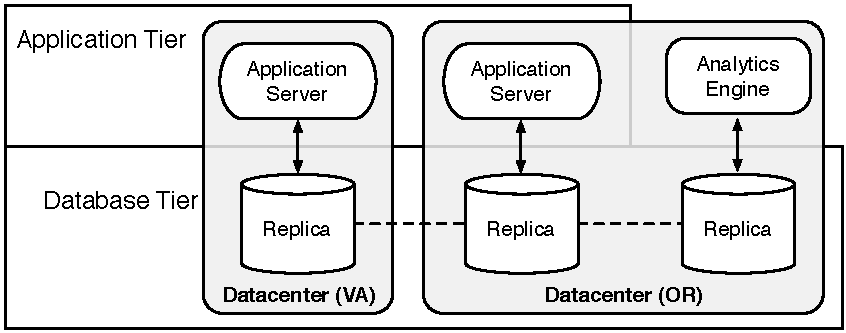
\includegraphics[width=\figscale\columnwidth]{diagram/servers.pdf}
\vspace{.5em}
\caption{An illustration of a distributed, replicated database and its
  relation to application servers and end users. In modern distributed
  databases, data is stored on several servers that may be located in
  geographically distant regions (e.g., Virginia and Oregon, or even
  different continents) and may be accessed by multiple database
  clients (e.g., application servers, analytics frameworks, database
  administrators) simultaneously. The key challenge that we
  investigate in this thesis is how to minimize the amount of
  synchronous communication across databases while providing ``always
  on,'' scalable, and high performance access to each replica.}
\label{fig:servers}
\end{figure}

In this work, we investigate a conceptually simple class of designs
for robust distributed databases: we study the design of databases
that allow applications to make non-trivial progress independent of
network behavior. That is, we study the design of database systems
that provide \textit{coordination-free} execution: whenever database
clients can access at least one copy of database state, they are
guaranteed to make non-trivial progress. This means that, in the
presence of communication failures between servers, each client's
operations may still proceed, providing ``always on'' functionality,
or guaranteed \textit{availability}. Even when database servers are
able to communicate with one another, communication is not
required. This allows \textit{low latency} operation: each client's
requests can be processed using locally accessible resources. Finally,
coordination-free execution ensures \textit{scalability}: as more
servers are added, the database can make use of them without
disrupting existing servers. This results in increased capacity. Thus,
coordination-free execution offers attractive performance and
availability benefits while ensuring that, subject to the availability
of additional resources, additional requests can be serviced on
demand.

This coordination-free database system design represents a departure from
classic database system designs. Traditionally, database systems
exposed a \textit{serializable transaction} interface: if user
operations are bundled into transactions, or groups of multiple
operations over multiple data items, a database providing
\textit{serializability} guarantees that the result of executing the
transactions is equivalent to some serial execution of the
transactions~\cite{bernstein-book}. Serializability is remarkably
convenient for programmers, who do not need to reason about
concurrency or distribution. However, serializability is inconvenient
for databases: serializability (provably) requires
coordination~\cite{davidson-survey}, negating the benefits of
coordination-free execution. Intuitively, enforcing a serial ordering
between transactions precludes the ability to guarantee
the transactions' independent progress when executed on multiple
servers.

As a result, increased application demands for availability, low
latency, and scalability have led to a recent schism within mainstream
database system designs~\cite{marcus-talk,mohan-note}.  A
proliferation of database systems, often called ``NoSQL'' systems,
forego serializability (and other ``strong'' semantics) in order to
provide coordination-free execution. However, in turn, these NoSQL
systems provide few, if any semantic guarantees about their query
results and about database state (also called \textit{safety
  properties}; e.g., ``no two users share a
username'')~\cite{queue,bernstein-survey,lamport-safety}. In contrast
with serializability, which guarantees that safety properties
preserved by individual transactions will be preserved under their
serial composition, these NoSQL stores leave the enforcement of
application safety to the application---a challenging and error-prone
proposition~\cite{consistency-borders,entitygroup}. Thus, database users and application programmers today
are left with one of two options: ensure safety via serializability
and coordination, or forego safety within the database but enjoy the benefits of
coordination-free execution.

In this thesis, we examine this apparent tension between ensuring
application safety properties within the database and enjoying the
scalability, availability, and performance benefits of
coordination-free execution. Is enforcing safety properties always at
odds with coordination-free execution? If we rely on serializability,
the answer is yes. Instead, we consider an alternative: the
enforcement of non-serializable semantic guarantees in a
coordination-free manner. By examining the safety properties of
today's database-backed applications, we determine whether
coordination is strictly necessary to enforce them and explore
implementations that limit the use of coordination. Thus, this thesis
explores the relationship between correctness---according to useful
safety guarantees---and coordination. More precisely, what is the
coordination cost of a given safety guarantee? What is the minimum
communication we must perform to enforce various correctness criteria?

\section{Coordination Avoidance}

Our primary goal in this thesis is to build database systems that
coordinate only when strictly required in order to guarantee
application safety. To realize this goal, we examine which semantic
guarantees databases \textit{can} provide under coordination-free
execution---and explore implementations that fulfill this
potential. We study a range of guarantees from both classic database
systems as well as guarantees required by modern database-backed
applications. Today, most of these guarantees are either implemented
using coordination or are not provided by coordination-free
systems. However, we demonstrate that many of these requirements can
be correctly implemented without coordination and provide algorithms
and system implementations for doing so. This enables what we call
\textit{coordination avoidance}: the use of as little coordination as
possible while maintaining safety guarantees on behalf of database
users.

\vspace{0.5em}
\noindent\textbf{Thesis Statement:} \textit{Many semantic requirements
  of database-backed applications can be efficiently enforced without
  coordination, thus improving scalability, latency, and
  availability.}

To achieve this goal, we first develop a new, general rule for
determining whether a coordination-free implementation of a given
safety property exists, called \textit{\iconfluence}. Informally,
\iconfluence determines whether the result of executing operations on
independent copies of data can be combined (or ``merged'') into a
single, coherent (i.e., \textit{convergent}) copy of database
state. Given a set of operations, a safety property that we wish to
maintain over all copies of database state, and a merge function,
\iconfluence tells us whether coordination-free execution is
possible. \Iconfluence is both necessary and sufficient: if
\iconfluence holds, a coordination-free, convergent implementation
exists. If \iconfluence does not hold, no system can implement the
semantics while also providing coordination-free, convergent
execution.

Given this \iconfluence criterion, we examine a set of common semantic
guarantees found in database systems and database-backed applications
today to determine whether a coordination-free execution strategy for
enforcing them exists. We perform several case studies, which we
describe in detail below. In many cases, although existing
implementations of these guarantees may rely on coordination, we show
that coordination-free implementations of the semantics exist. This
provides the scalability, performance, and availability benefits of
coordination-free execution---but without compromising desirable
semantic guarantees. None of these guarantees is serializable, but all
of them correspond to existing or emerging demands from
applications today.

Our use of \iconfluence recognizes latent potential for
coordination-free execution in existing and emerging applications. In
demonstrating this potential, we highlight a need for conscientious
consideration of coordination in the design of database systems: in
many \iconfluent scenarios, traditional and/or legacy implementations
designed for non-distributed environments over-coordinate and fail to
capture the potential for coordination-free execution. Conversely,
when \iconfluence does not hold, understanding when a
coordination-free implementation does not exist spares system
designers the effort of searching for a more efficient implementation
when in fact such an implementation does not exist.

Of course, simply recognizing that a coordination-free implementation
exists does not by itself lead to coordination-free systems. Rather,
we must also find a coordination-free implementation of \iconfluent
semantics. Therefore, we present the design, implementation, and
evaluation of several sets of \iconfluent guarantees. We demonstrate
order-of-magnitude improvements in latency and throughput over
traditional algorithms, validating the power of coordination-free
systems design. In addition to these case studies, we also present
more general design principles for realizing coordination avoidance in
practice. We note the importance of separating visibility from
progress, ensuring composability of operations, and controlling
visibility via multiversioning.

\minihead{By example} As a simple example, consider the common Read
Committed (RC) isolation guarantee~\cite{adya}, which is the default
semantics in fifteen of eighteen popular relational databases,
including Oracle, SAP Hana, and Microsoft SQL Server
(Chapter~\ref{c.isolation}). Informally, Read Committed ensures that
users never read non-final writes to data; if, within a transaction, a
user sets her username to ``Sally'' and, subsequently, sets her
username to ``Sal,'' no other user should ever read that the user's
username is ``Sally.'' The classic strategy for implementing Read
Committed isolation dates to the 1970s and relies on locking: when our
user wants to update her username record, she acquires a mutually
exclusive lock on the record~\cite{gray-isolation}. This is a
reasonable strategy for a single-node database, but the coordination
required to implement this mutual exclusion can be disastrous in a
modern distributed environment: while our first user holds the lock on
her username record, all other users who wish to also access the same
username record must wait.

While coordination is sufficient to enforce RC isolation (via
locking), is it strictly necessary? We can apply the principle of
\iconfluence here: informally, if each individual user never observes
non-final writes (i.e., each individual read-write history is valid
under RC isolation), then their collective behavior (i.e., the
``merged'' histories) will not exhibit any reads of non-final
writes. Thus, insofar as each individual user respects RC isolation,
all users will, and so it is \iconfluent. As a result, there must be a
coordination-free algorithm for enforcing RC isolation; now we must
find one. One strategy is to store multiple versions of each record
and mark each version with a special bit recording whether the
corresponding write is a final write or not. If the database only
shows users records that have been marked as final writes upon
transaction commit, users will never observe non-final
writes. Moreover, users can create versions, mark them as final, and
read versions marked as final entirely concurrently, on separate
copies of state, achieving our goal of a coordination-free
implementation of RC isolation.

While this example is relatively simple, it demonstrates the power of
rethinking legacy implementations of important semantics. In
Chapter~\ref{c.isolation}, we demonstrate how a slightly modified
protocol achieves orders of magnitude improvements in performance on
modern cloud computing infrastructure.\vspace{.5em}

In the remainder of this chapter, we outline the key contributions of
this work and describe the structure of the remainder of this thesis.

\section{Primary Contributions}

\begin{figure}[t!]
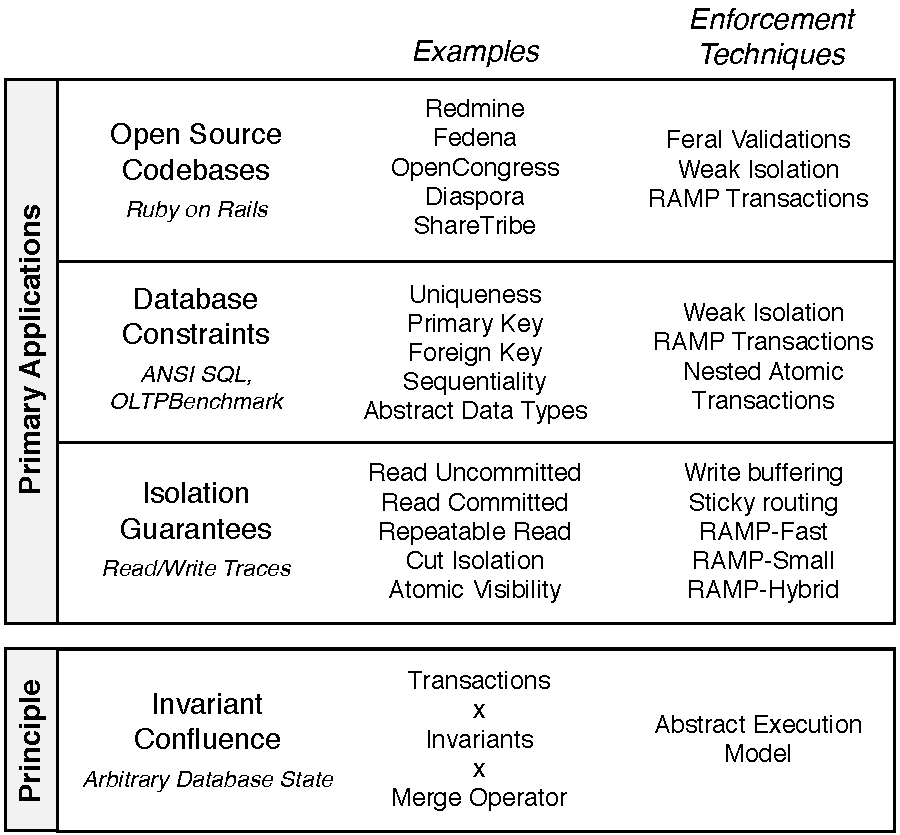
\includegraphics[width=\figscale\columnwidth]{diagram/contributions.pdf}
\vspace{.75em}
\caption{In this thesis, we develop the principle of \IConfluence, a
  necessary and sufficient condition for safe, convergent,
  coordination-free execution, and apply it to a range of application
  domains at increasing levels of abstraction: database isolation,
  database constraints, and safety properties from modern
  database-backed applications. Each guarantee that is \iconfluent is
  guaranteed to have at least one coordination-free implementation; we
  investigate the design of several implementations in this work,
  which operate at the database infrastructure tier (Figure~\ref{fig:servers}).}
\label{fig:contribs}
\end{figure}


In this section, we summarize the primary contributions of this work.

\newcommand{\contribution}[1]{\vspace{.5em}\noindent\textbf{#1}.\xspace\xspace}
%\begin{itemize}[label={}]
 \contribution{Coordination-free execution and \IConfluence}  We identify coordination-free execution as fundamental to available,
 low latency, and scalable system execution. To do so, we present a
 system model and show a direct correspondence between these desirable
 system properties and the ability to guarantee non-trivial progress
 in an asynchronous network.

 We subsequently develop the \iconfluence property, a necessary and
 sufficient condition for ensuring that a safety guarantee can be
 guaranteed under coordination-free, convergent execution of a given
 set of transactions. This is the first necessary and sufficient
 condition for these properties that we have encountered. In effect,
 \iconfluence lifts traditional partitioning arguments from
 distributed systems from the domain of event traces to the domain of
 arbitrary application logic and constraints over data. We use this
 property to examine and optimize a range of semantics from database
 systems (Figure~\ref{fig:contribs}), which we describe in turn below.

 \contribution{Coordination-free Isolation Guarantees} While
 transactional guarantees are often associated with serializability
 and its necessarily coordinated implementations, most databases in
 practice provide weaker forms of transactional isolation, or variants
 of admissible read-write interleavings (Figure~\ref{fig:contribs}).
 In a survey of 18 ``ACID'' and ``NewSQL'' databases, we find that
 only three offered serializability by default and only nine offered
 it as as an option at all. We investigate the weaker models offered
 by these databases and show that many are \iconfluent. For example,
 common isolation models such as Read Committed (default in eight
 databases) and ANSI Repeatable Read isolation are \iconfluent. Many
 guarantees, like Read Committed, arbitrated \textit{visibility} but
 not concurrency (much like causal consistency). The resulting
 taxonomy is one of the first unified treatments of weak isolation,
 distributed register consistency, session guarantees, and
 coordination requirements in the literature. Using these results, we
 implement a coordination-free prototype implementing weak isolation
 guarantees that achieves up to two order-of-magnitude latency
 reductions when deployed across datacenters.

  In addition to investigating existing isolation guarantees, we
  examine new guarantees. A number of applications leverage
  database-provided functionality for enforcing referential integrity,
  secondary indexing, and multi-get and multi-put operations, yet
  there is no coordination-free mechanism for enforcing
  them. Accordingly, a number of practitioner reports on systems
  (e.g., from Facebook, Google, LinkedIn, and Yahoo!) specifically
  highlight these use cases as scenarios where, lacking a
  coordination-free algorithm, architects explicitly sacrificed
  correctness for latency and availability. In response, we develop a
  new, \iconfluent isolation model called Read Atomic (RA) isolation 
  and set of scalable, coordination-free algorithms called Read Atomic
  Multi-Partition (RAMP) Transactions for addressing the isolation
  requirements of these use cases. Informally, RA guarantees
  \textit{atomic visibility} of updates: once one write from a
  transaction is visible, all writes will be visible. Existing
  protocols for achieving RA isolation (or stronger), such as distributed
  locking, couple atomic visibility with mutual exclusion; RAMP
  achieves the former without the cost of the latter. RAMP uses
  limited multi-versioning to allow clients to operate concurrently
  over the same data items while ensuring that readers can correctly
  detect and repair incomplete writes. Across a range of workloads
  (including high contention scenarios), RAMP transactions incur
  limited overhead and outperform existing mechanisms for achieving RA isolation
  while scaling linearly.

  \contribution{Coordination-free Database Constraints and Application
    Criteria} Moving from read-write traces to higher-level semantic
  properties (Figure~\ref{fig:contribs}), we examine the integrity
  constraints and invariants offered by databases today---including
  the foreign key constraints addressed by RAMP but also row-level
  check constraints, uniqueness constraints, and constraints on
  abstract data types---and classify each as \iconfluent or not. Many
  are \iconfluent, so we subsequently apply this classification to a
  number of database workloads from the OLTPBenchmark
  suite~\cite{oltpbench}. Many invariants in these workloads pass the
  \iconfluence test as well. For example, in the TPC-C benchmark, the
  gold standard for transaction processing performance, ten of twelve
  invariants are \iconfluent under the workload. Given this
  classification, we develop a database prototype and
  coordination-avoiding execution strategy for TPC-C that, on a
  cluster of 200 servers, achieves a 25-fold improvement in throughput
  over the prior best result (over 12.7M New-Order transactions per
  second).

  While we are able to find \iconfluent database integrity constraints
  and benchmarks, are \textit{real} applications \iconfluent?
  Moreover, are invariants a practical choice of correctness criteria?
  To answer these questions, we examine open source web applications
  to inspect their safety properties (Figure~\ref{fig:contribs}). We
  find that popular web programming frameworks---including Ruby on
  Rails, Django, and Spring/Hibernate---have introduced support for
  \textit{validations}, or declarative, application-level
  invariants. We subsequently analyze the use of validations in 67 of
  the most popular Ruby on Rails applications on GitHub and find that,
  in fact, validation usage is fourteen times more common than the use
  of database transactions. Moreover, more than 86.9\% (of over 9900
  invariants) are \iconfluent. However, the remainder are \textit{not}
  \iconfluent and therefore require coordination. For these
  invariants, we profile the incidence of constraint violations both
  with and without validations. In addition to demonstrating the
  applicability of \iconfluence, this study exposes a surprising
  practitioner trend away from transactions towards using invariants via
  validations.\vspace{.5em}

  In all, these results highlight a widespread potential for
  coordination-avoiding database system design within both classic and
  emerging database-backed applications. While coordination cannot
  always be avoided, in many common scenarios, we find it is possible to
  guarantee application safety within the database while also
  providing coordination-free execution. Our resulting database system
  prototypes and their regular order-of-magnitude speedups compared to
  conventional approaches evidence the power of this latent potential
  for coordination-avoiding execution.

\begin{comment}
   In addition to the above, we present a summary of additional results
  developed during our investigation of coordination avoidance,
  including: PBS, a new methodology for profiling the incidence of
  isolation violations in weakly consistent stores; the Bolt-on
  Architecture for upgrading the isolation of underlying eventually
  consistent data stores as well as an implementation of bolt-on
  causal consistency; Explicit Causality, an API for reducing the
  overheads of causal information tracking; and early results from
  applying coordination-avoiding execution to the tasks of distributed
  convex optimization and model serving and maintenance.
\end{comment}

\section{Outline and Previously Published Work}

The remainder of this dissertation proceeds as
follows. Chapter~\ref{c.background} provides background on
coordination and defines our system model. Chapter~\ref{c.iconfluence}
presents the \IConfluence
property. Chapters~\ref{c.isolation},~\ref{c.ramp},and~\ref{c.constraints}
examine the coordination requirements and coordination-free
implementations of transaction isolation, database functionality such
as indexes, and constraints. Chapter~\ref{c.relatedwork} discusses
related work and Chapter~\ref{c.conclusion} concludes with a
discussion of lessons learned, topics for future work, and closing
thoughts.

Chapter~\ref{c.background} includes material from several previous
publications~\cite{hat-vldb,coord-avoid,partitions-queue14,queue,pbs,pbs-vldbj2013,pbs-demo-sigmod2013}. Chapter~\ref{c.iconfluence}
revises material from~\cite{coord-avoid}. Chapter~\ref{c.isolation}
revises~\cite{hat-vldb} and~\cite{hat-hotos}. Chapter~\ref{c.ramp}
revises~\cite{ramp-sigmod14} and includes material
from~\cite{explicit-socc}. Chapter~\ref{c.constraints} revises
material from~\cite{coord-avoid} and~\cite{apps} and includes material
from~\cite{bolton}. Chapter~\ref{c.conclusion} includes material
from~\cite{velox-overview,admm}.


\begin{comment}
\section{Note on Exposition}

The goal of this thesis is the improved design of modern distributed
database systems. In doing so, we pursue a principled approach to
systems design that provides rigorous rationale for
\textit{why} a given system design is preferable (or at least
outperforms existing systems along some dimension, whether latency,
scalability, availability, or throughput); in this thesis, our primary
guiding principle is the pursuit of coordination-free execution. To
assist in this pursuit of principle, we adopt a modest amount of
formalism for the analysis of both semantics and our proposed
algorithms. Thus, while our ultimate objectives lie in the realm of
systems, we leverage machinery from more formal domains.

In our exposition, we have largely opted to present the systems
rationale and explanations first, followed by their respective
formalization and more rigorous treatment. To keep each chapter
self-contained, we have included the more formal components in the
body of each chapter (i.e., instead of in an appendix). However, we
have delineated each more formal section with an appropriate
heading. Readers with a more practical inclination may wish to skip
these sections upon first reading. Readers with a more formal
inclination may wish to pursue an alternative section ordering than we
have chosen here. Any ambiguities in the less formal prose should be
resolvable by consulting the more formal text.
\end{comment}

\newcommand{\ttf}[1]{\texttt{#1}\xspace}
\newcommand{\dpc}{\ttf{D-2PC}}
\newcommand{\cpc}{\ttf{C-2PC}}

\chapter{Coordination: Concepts and Costs}
\label{c.background}

In this chapter, we further examine the concept of coordination and
why we seek to avoid it. We discuss traditional uses of coordination
to maintain correct data in database systems and measure its costs in
modern distributed environment, which we will attempt to circumvent in
the remainder of this thesis. We also present our formal system model
for replicated databases.

\section{Coordination and Correctness in Database Systems}
\label{sec:t-motivation}
As repositories for application state, databases are traditionally
tasked with maintaining, informally, ``correct'' data---that is, data
that obey some semantic guarantees about their integrity---on behalf
of users. Thus, during concurrent access to data, a database ensuring
data correctness must therefore decide which user operations can
execute simultaneously and which, if any, cannot. Informally, we say
that two operations within a database must \textit{coordinate} if they
cannot execute concurrently on independent copies of the database state
(Section~\ref{sec:model} provides a more formal treatment).

\minihead{By example} Consider a database-backed payroll application
that maintains information about employees and departments within a
small business. In the application, $a.)$ each employee is assigned a
unique ID number and $b.)$ each employee belongs to exactly one
department. A database ensuring correctness must maintain these
application-level semantic guarantees (or data \textit{invariants}) on
behalf of the application (i.e., without application-level
intervention). In our payroll application, this is non-trivial: for
example, if the application attempts to simultaneously create two
employees by examining the set of currently assigned IDs and choosing
an unassigned ID for each new employee, then the database must ensure
the employees are assigned distinct IDs.

\minihead{Serializability and conflicts} The classic answer to
maintaining application-level invariants is to use serializable
isolation: execute each user's ordered sequence of operations, or
\textit{transactions}, such that the end result is equivalent to some
sequential execution~\cite{tamer-book,bernstein-book,gray-virtues}. If
each transaction preserves correctness in isolation, composition via
serializable execution ensures correctness. In our payroll example,
the database would execute the two employee creation transactions such
that one transaction appears to execute after the other. The second
transaction would observe the ID that the first transaction chose,
thus avoiding duplicate ID assignment.

While serializability is a powerful abstraction, it comes with a cost:
for arbitrary transactions (and for all implementations of
serializability's more conservative variant---conflict
serializability), any two operations to the same item---at least one
of which is a write---will result in a \textit{read/write
  conflict}. Under serializability, these conflicts require
coordination: to provide a serial ordering, conflicts must be totally
ordered across transactions, and so transactions cannot proceed
entirely independently~\cite{bernstein-book}. As a canonical example,
given initial database state containing two variables $x$ and $y$,
where $\{x=\bot, y=\bot\}$, if transaction $T_1$ reads from $y$ and
writes $x=1$ and and $T_2$ reads from $x$ and writes $y=1$, then a
database cannot both execute $T_1$ and $T_2$ independently on separate
copies of state while maintaining
serializability~\cite{davidson-survey,hat-vldb}.\footnote{This
  read-write pattern might arise in our ID assignment scenario: $T_1$
  attempts to reserve ID $1$ for its user, $x$, while $T_2$ attempts
  to reserve ID $1$ for its user, $y$. If the two transactions run
  concurrently on separate copies of the database, neither $T_1$ nor
  $T_2$ would observe the others's updates. We present this example in
  terms of reads and writes because it is standard and to highlight
  the fact that serializability enforces concurrency by examining
  read/write access to variables, not by examining the program
  semantics.}

Because serializable semantics require coordination, \textit{all}
database implementations that provide serializability will
coordinate. For example, a database could use two-phase
locking~\cite{gray-isolation} to provide serializability: in a
simplified protocol, the first time a transaction accesses a data
item $x$, the transaction can acquire an exclusive lock on $x$; once
the transaction has completed all of its operations on the database,
it can release all of its locks. In this protocol, locks form a point
of coordination between concurrent transactions: while one transaction
holds an exclusive lock on an item, other transactions that wish to
operate on the same item cannot make progress.

\minihead{Semantics, Sufficiency, and Necessity} It is often
convenient to reason about semantic guarantees instead of concrete
implementations of those guarantees. Instead of examining concurrency
control mechanisms one-by-one (e.g., multi-version concurrency
control, optimistic concurrency control, pre-scheduling, and so on),
we can unequivocally determine---as in the case of
serializability---that all implementations of a given semantics
require coordination to enforce.

However, the converse does not hold: just because a given
implementation of a guarantee uses coordination does not mean that the
guarantee necessarily requires coordination for enforcement. For
example, even though a database may employ serializability to enforce
an invariant, the invariant may not \textit{require} coordination for
correct enforcement. There may or may not be ways to enforce the
invariants without coordination. In general, we can always
coordinate. The core question is whether coordination is necessary for
a given invariant or semantic property.

\section{Understanding the Costs of Coordination}

Why worry about coordination? Peter Deutsch starts his classic list of
``Fallacies of Distributed Computing'' with two concerns fundamental
to distributed database systems: ``\textit{1.)}  The network is
reliable. \textit{2.)} Latency is zero''~\cite{fallacies-deutsch}. In
a distributed setting, network failures may prevent database servers
from communicating, and, in the absence of failures, communication is
slowed by factors like physical distance, network congestion, and
routing. Thus, as we discuss here, the costs of coordination can be
observed across three primary dimensions: increased latency, decreased
throughput, and, in the event of partial failures, unavailability. In
this section, we examine these costs in detail.


\subsection{Latency}
\label{sec:latency}

Even with fault-free networks, distributed systems face the challenge
of network communication latency. If two operations running on two
separate servers must coordinate, then the latency experienced by the
operations will be bounded from below by the amount of time required to
exchange information between the sites. In this section, we quantify
network latencies of modern cloud computing environments. These are
often large and may exceed hundreds of milliseconds in a
geo-replicated, multi-datacenter context.  Fundamentally, the speed at
which two servers can communicate is (according to modern physics)
bounded by the speed of light. In the best case, two servers on
opposite sides of the Earth communicating via a hypothetical link
through the planet's core would require a minimum 85.1~ms round-trip
time (RTT; 133.7~ms if sent at surface level). As services are
replicated to multiple, geographically distinct sites, the cost of
communication between replicas increases.

\definecolor{min-lat-color}{HTML}{B2FF99}
\definecolor{max-lat-color}{HTML}{FF7F7F}

\begin{table}[t!]

\subfloat[Within \texttt{us-east-b} availability zone] {
  \makebox[.5\textwidth]{
 \begin{tabular}{|c|c|c|}\hline
 & \multicolumn{1}{c}{H2} & \multicolumn{1}{c|}{H3}\\\hline
H1  & 0.55   & \colorbox{max-lat-color}{0.56} \\
H2 &  & \colorbox{min-lat-color}{0.50}  \\
\hline
  \end{tabular}}
 }
\subfloat[Across \texttt{us-east} availability zones]{
  \makebox[.5\textwidth]{
    \begin{tabular}{|c|c|c|}\hline
 & \multicolumn{1}{c}{C} & \multicolumn{1}{c|}{D}\\\hline
B & \colorbox{min-lat-color}{1.08} & 3.12 \\
C & & \colorbox{max-lat-color}{3.57}  \\
\hline
  \end{tabular}}
}\vspace{.5em}

\subfloat[Cross-region (CA:~California, OR:~Oregon, VA:~Virginia, TO:~Tokyo, IR:~Ireland, SY:~Sydney, SP:~S\~{a}o Paulo, SI:~Singapore)] {
  \begin{tabular}{|c|c|c|c|c|c|c|c|c|}
\hline
& \multicolumn{1}{c}{OR} & \multicolumn{1}{c}{VA} & \multicolumn{1}{c}{TO} & \multicolumn{1}{c}{IR} & \multicolumn{1}{c}{SY} & \multicolumn{1}{c}{SP} & \multicolumn{1}{c|}{SI} \\\hline
CA & \colorbox{min-lat-color}{22.5}   & 84.5   & 143.7   & 169.8   & 179.1   & 185.9   & 186.9  \\
OR &  & 82.9   & 135.1   & 170.6   & 200.6   & 207.8   & 234.4  \\
VA & &  & 202.4   & 107.9   & 265.6   & 163.4   & 253.5  \\
TO & & &  & 278.3   & 144.2   & 301.4   & 90.6  \\
IR & & & &  & 346.2   & 239.8   & 234.1  \\
SY & & & & &  & 333.6   & 243.1  \\
SP & & & & & &  & \colorbox{max-lat-color}{362.8}  \\
\hline
  \end{tabular}\vspace{.5em}
}\vspace{1em}

\caption{Mean RTT times on EC2 (min and max highlighted)}
\label{table:rtt}
\end{table}

\begin{figure}[t!]
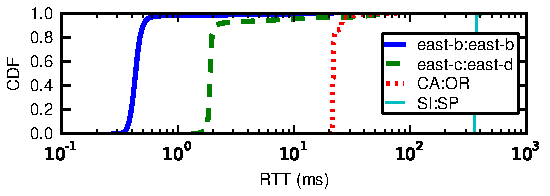
\includegraphics[width=\figscale\columnwidth]{figs/ping-plot.pdf}\vspace{.5em}
\caption{CDF of round-trip times for slowest inter- and intra-
  availability zone links compared to cross-region links.}
\label{fig:rtt}
\end{figure}

In actual server deployments, messages travel slower than the speed of
light due to routing, congestion, and computational overheads. To
illustrate the behavior of intra-datacenter, inter-datacenter, and
inter-planetary networks, we performed a measurement study of network
behavior on Amazon's Elastic Compute Cloud (EC2), a widely used public
compute cloud. We measured one week of ping times (i.e., round-trip
times, or RTTs) between all seven EC2 geographic ``regions,'' across
three ``availability zones'' (closely co-located datacenters), and
within a single ``availability zone'' (datacenter), at a granularity
of 1s. We summarize the results of our network measurement study in
Table~\ref{table:rtt}. On average, intra-datacenter communication
(Table~\ref{table:rtt}a) is between 1.82 and 6.38 times faster than
across geographically co-located datacenters (Table~\ref{table:rtt}b)
and between 40 and 647 times faster than across geographically
distributed datacenters (Table~\ref{table:rtt}c). The cost of
wide-area communication exceeds the speed of light: for example, while
a speed-of-light RTT from S\~{a}o Paulo to Singapore RTT is 106.7~ms,
ping packets incur an average 362.8~ms RTT (95th percentile: 649~ms). As
shown in Figure~\ref{fig:rtt}, the distribution of latencies varies
between links, but the overall trend is clear: coordination may lead
to substantial delays. Quantifying and minimizing communication delays
is also an active area of research in the networking
community~\cite{bobtail}.

\subsection{Throughput and Scalability}
\label{sec:background-cmotivation}

Coordination also affects throughput. If a transaction takes $d$
seconds to execute, the maximum throughput of coordinating
transactions operating on the same items under a general-purpose
(i.e., interactive, non-batched) transaction model is limited by
$\frac{1}{d}$. Any operations that arrive in excess of this limit will
also have to wait. Within a single server, delays can be small,
permitting tens to hundreds of thousands of conflicting transactions
per item per second. In a partitioned database system, where different
items are located on different servers, or in a replicated database
system, where the same item is located (and is available for
operations) on multiple servers, the cost increases: delay is
lower-bounded by network latency. On a local area network, delay may
vary from several microseconds (e.g., via Infiniband or RDMA) to
several milliseconds on today's cloud infrastructure, permitting
anywhere from a few hundred transactions to a few hundred thousand
transactions per second. However, as we have seen, a wide-area
network, delay is lower-bounded by the speed of light (worst-case on
Earth, around 75~ms, or about 13 operations per
second~\cite{hat-vldb}). Under network
partitions~\cite{queue-partitions}, as delay tends towards infinity,
these penalties lead to unavailability~\cite{gilbert-cap,hat-vldb}. In
contrast, operations executing without coordination can proceed
concurrently and will not incur these penalties.

To further understand the costs of coordination, we performed two sets
of measurements---one using a database prototype and one using traces
from prior studies.  We first compared the throughput of a set of
coordinated and coordination-free transaction execution. Our basic
workload is simple: a set of transactions read and increment a set of
integers stored on separate servers.


First, we implemented two coordinated algorithms: traditional
two-phase locking and an optimized variant of two-phase locking, both
on in-memory data. In two-phase locking, each client acquires locks
one at a time, requiring a full round trip time (RTT) for every lock
request. For an $N$ item transaction, locks are held for $2N+1$
message delays (the $+1$ is due to broadcasting the unlock/commit
command to the participating servers). Our optimized two-phase locking
only uses one message delay (half RTT) to perform each lock request:
the client specifies the entire set of items it wishes to modify at
the start of the transaction (in our implementation, the number of
items in the transaction and the starting item ID), and, once a server
has updated its respective item, the server forwards the remainder of
the transaction to the server responsible for the next write in the
transaction (similar to linear commit
protocols~\cite{bernstein-book}). For an $N$-item transaction, locks
are only held for $N$ message delays (the final server both broadcasts
the unlock request to all other servers and also notifies the client),
while a $1$-item transaction does not require distributed locking.

To avoid deadlock (which we found was otherwise common in this
high-contention microbenchmark), our implementation totally orders any
lock requests according to item and executes them sequentially (e.g.,
lock item $1$ then lock item $2$ and so on). Our implementation also
piggybacks operation commands along with lock requests, further
avoiding message delays. Since we are only locking one item per
server, our microbenchmark code does not use a dynamic lock manager
and instead associates a single lock with each item; this further
lowers locking overheads.

Our coordination-free transaction implementation is simpler: it uses
no locks and simply performs the increment operation across each
transaction in parallel, without acquiring locks.

We partitioned eight in-memory items (integers) across eight
\texttt{cr1.8xlarge} Amazon EC2 instances with clients located on a
separate set of \texttt{cr1.8xlarge}
instances. Figure~\ref{fig:micro-all} reported in depicts results for
the coordination-free implementation and the optimized two-phase
locking case. Unsurprisingly, two-phase locking performs worse than
optimized two-phase locking, but both incur substantial penalties due
to coordination delay over the network.

\begin{figure}
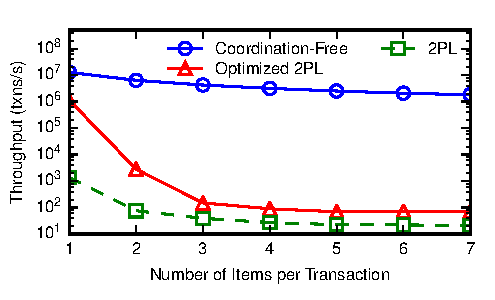
\includegraphics[width=\figscale\columnwidth]{figs/micro_thru_all.pdf}
\caption{Microbenchmark performance of coordinated and
  coordination-free execution of transactions of varying size writing
  to eight items located on eight separate multi-core servers.}
\label{fig:micro-all}
\end{figure}

With single-item, non-distributed transactions, the coordination-free
implementation achieves, in aggregate, over 12M transactions per
second and bottlenecks on \textit{physical resources}---namely, CPU
cycles. In contrast, the lock-based implementation achieves
approximately $1.1$M transactions per second: it is unable to fully
utilize all 32 multi-core processor contexts due to lock contention. For
distributed transactions, coordination-free throughput decreases
linearly (as an $N$-item transaction performs $N$ writes), while the
throughput of coordinating transactions drops by over three orders of
magnitude.

While the above microbenchmark demonstrates the costs of a particular
\textit{implementation} of coordination, we also studied the
effect of more fundamental, implementation-independent overheads
(i.e., also applicable to optimistic and scheduling-based concurrency
control mechanisms). We determined the maximum attainable throughput
for coordinated execution within a single datacenter (based on data
from~\cite{bobtail}) and across multiple datacenters (based on data
from~\cite{hat-vldb}) due to blocking coordination during atomic
commitment~\cite{bernstein-book}. 

We simulate traditional two-phase commit~\cite{bernstein-book} and
decentralized two-phase commit~\cite{paxos-commit} using network
models derived from existing studies. For an $N$-server transaction,
classic two-phase commit (\cpc) requires $N$ (parallel) coordinator to
server RTTs, while decentralized two-phase commit (\dpc) requires $N$
(parallel) server to server broadcasts, or $N^2$ messages. Our
simulation is straightforward, but we make several
optimizations to improve the throughput of each algorithm. First, we
assume that transactions are pipelined, so that each server can
\texttt{prepare} immediately after it has \texttt{commit}ted the prior
transaction. Second, our pipelines are ideal in that we do not
consider deadlock: only one transaction \texttt{prepare}s at a given
time. Third, we do not consider the cost of local processing of each
transaction: throughput is determined entirely by communication delay.

Figure~\ref{fig:2pc} shows that, in the local area, with only two
servers (e.g., two replicas or two coordinating operations on items
residing on different servers), throughput is bounded by 1125
transactions per second (via \dpc; 668 transactions per second via
\cpc). Across eight servers, \dpc throughput drops to 173 transactions
per second (respectively 321 for \cpc) due to long-tailed latency
distributions. In the wide area, the effects are more severe: if
coordinating from Virginia to Oregon, \dpc message delays are 83~ms
per commit, allowing 12 operations per second. If coordinating between
all eight EC2 availability zones, throughput drops to slightly over 2
transactions per second in both algorithms.

These results should also be unsurprising: coordinating---especially over
the network---can incur serious throughput penalties. In contrast,
coordination-free operations can execute without incurring these
costs. The costs of actual workloads can vary: if coordinating
operations are rare, concurrency control will not be a bottleneck. For
example, a serializable database executing transactions with disjoint
read and write sets can perform as well as a non-serializable database
without compromising correctness~\cite{shore-communication}. However,
as these results demonstrate, minimizing the amount of coordination
and its degree of distribution can therefore have a tangible impact on
performance, latency, and
availability~\cite{pacelc,hat-vldb,gilbert-cap}. While we study real
applications in Section~\ref{sec:evaluation}, these measurements
highlight the worst of coordination costs on modern hardware.

\begin{figure}
  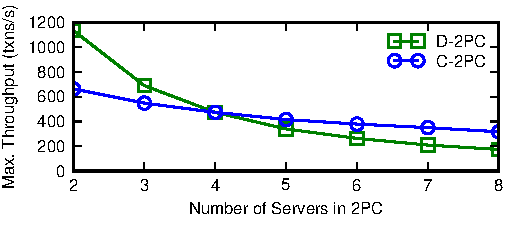
\includegraphics[width=.8\columnwidth]{figs/singledc-twopc.pdf}\\
  {\centering {\small a.) Maximum serializable transaction
      throughput over local-area network in~\cite{bobtail}}\par}
  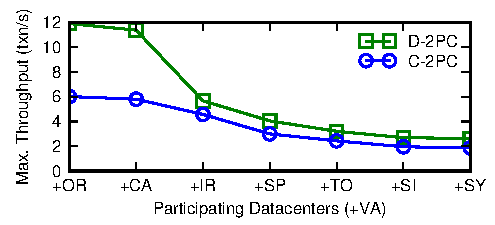
\includegraphics[width=.8\columnwidth]{figs/multidc-twopc.pdf}\\
  {\small b.) Maximum serializable transaction throughput
    over wide-area network in~\cite{hat-vldb} with transactions
    originating from a coordinator in Virginia (VA; OR:~Oregon,
    CA:~California, IR:~Ireland, SP:~S\~{a}o Paulo, TO:~Tokyo,
    SI:~Singapore, SY:~Sydney)}\vspace{1em}

  \caption{Atomic commitment latency as an upper bound on conflicting
    serializable transaction throughput over local-area and wide-area networks.}
\label{fig:2pc}
\end{figure}

While this study is based solely on reported latencies, deployment
reports corroborate our findings. For example, Google's F1 uses
optimistic concurrency control via WAN with commit latencies of $50$
to 150~ms. As the authors discuss, this limits throughput to between 6
to 20 transactions per second per data item~\cite{f1}. Megastore's
average write latencies of 100 to 400~ms suggest similar throughputs
to those that we have predicted~\cite{megastore}. Again,
\textit{aggregate} throughput may be greater as multiple 2PC rounds
for disjoint sets of data items may safely proceed in
parallel. However, \textit{worst-case} access patterns---in effect,
serial access to data items---will greatly limit throughput and
scalability. Adding more servers will not assist; parallel processing
is ineffective for workloads that must proceed serially.

\subsection{Availability and Failures}

According to James Hamilton, Vice President and Distinguished Engineer
on the Amazon Web Services team, ``network partitions should be rare
but net gear continues to cause more issues than it
should''~\cite{hamilton-partitions}. Anecdotal evidence confirms
Hamilton's assertion. In April 2011, a network misconfiguration led to
a twelve-hour series of outages across the Amazon EC2 and RDS
services~\cite{amazon-netpartition}. Subsequent misconfigurations and
partial failures such as another EC2 outage in October 2012 have led
to full site disruptions for popular web services like Reddit,
Foursquare, and Heroku~\cite{ec2-downsites}. At global scale, hardware
failures---like the 2011 outages in Internet backbones in North
America and Europe due a router bug~\cite{juniper-partition}---and
misconfigurations like the BGP faults in 2008~\cite{pakistan-youtube}
and 2010~\cite{research-experiment-partition} can cause widespread
partitioning behavior.

Many of our discussions with practitioners---especially those
operating on public cloud infrastructure---as well as reports from
large-scale operators like Google~\cite{dean-keynote} confirm that
partition management is an important consideration for service
operators today. System designs that do not account for partition
behavior may prove difficult to operate at scale: for example, less
than one year after its announcement, Yahoo!'s PNUTS developers
explicitly added support for weaker, highly available operation. The
engineers explained that ``strict adherence [to strong consistency]
leads to difficult situations under network partitioning or server
failures...in many circumstances, applications need a relaxed
approach''~\cite{pnuts-update}.

Several recent studies rigorously quantify partition behavior. A 2011
study of several Microsoft datacenters observed over 13,300 network
failures with end-user impact, with an estimated median 59,000 packets
lost per failure. The study found a mean of 40.8 network link failures
per day (95th percentile: 136), with a median time to repair of around
five minutes (and up to one week). Perhaps surprisingly, provisioning
redundant networks only reduces impact of failures by up to 40\%,
meaning network providers cannot easily curtail partition
behavior~\cite{sigcomm-dc}. A 2010 study of over 200 wide-area routers
found an average of 16.2--302.0 failures per link per year with an
average annual downtime of 24--497 minutes per link per year (95th
percentile at least 34 hours)~\cite{sigcomm-wan}. In HP's managed
enterprise networks, WAN, LAN, and connectivity problems account for
28.1\% of all customer support tickets while 39\% of tickets relate to
network hardware.  The median incident duration for highest priority
tickets ranges from 114--188 minutes and up to a full day for all
tickets~\cite{turner2012failure}. Other studies confirm these results,
showing median time between connectivity failures over a WAN network
of approximately 3000 seconds with a median time to repair between 2
and 1000 seconds~\cite{ip-backbone-failures} as well as frequent path
routing failures on the Internet~\cite{labovitz-failures}. A recent,
informal report by Kingsbury and Bailis catalogs a host of additional
practitioner reports~\cite{partitions-queue14}. Not surprisingly, isolating,
quantifying, and accounting for these network failures is an area of
active research in networking community~\cite{uw-failure-networks}.

\subsection{Summary: Costs}

Coordination is expensive. Empirical measurements on existing
infrastructure confirm its latency and throughput costs, and a host of
reports describe the difficulty of dealing with failures. Given an
absence of quantitative failure data, we focus primarily on the
performance-related aspects of coordination in this
dissertation. However, our pursuit of coordination avoidance benefits
all three dimensions.


\subsection{Outcome: NoSQL, Historical Context, Safety and Liveness}

The above costs have become especially pressing over the past decade,
leading to a schism among distributed database systems designers. An
increasing number of modern applications demand low latency and
available operation at unprecedented scale. For example, Facebook's
RocksDB reportedly handles nine billion queries per
second~\cite{rocks-tweet}, while increased latency may have a marked
impact on web application engagement and
revenue~\cite{google-talk,amazon-latency,perf-impact}. As a result,
the database market has been inundated by a large number of data stores
promising coordination-free execution (see
Chapter~\ref{c.relatedwork}). This market shift is perhaps the most
significant development in transaction processing over the past
decade.

While these stores, often collectively labeled ``NoSQL,'' provide
admirable scalability and behavioral properties, they infrequently
provide useful semantics for developers. That is, the common
denominator among these semantics is a particular property called
\textit{eventual consistency}: informally, if no additional updates
are made to a given data item, all reads to that item will eventually
return the same value~\cite{vogels-defs}. While this is a useful
property, it leaves some unfortunate holes. First, what is the
eventual state of the database? A database always returning the value
42 is eventually consistent, even if 42 was never written. The
database can eventually choose (i.e., \textit{converge to}) an
arbitrary value. Second, what values can be returned before the
eventual state of the database is reached? If replicas have not yet
converged, what guarantees can be made about the data returned?

To more precisely explain why eventual consistency is not strong
enough, we consider two concepts from distributed systems. A
\textit{safety} property guarantees that ``nothing bad happens'': for
example, every value that is read was, at some point in time, written
to the database. A \textit{liveness} property guarantees that
``something good eventually happens'': for example, all requests
eventually receive a response~\cite{liveness}. The difficulty with
eventual consistency is that it makes no safety guarantees---eventual
consistency is purely a liveness property. Something good eventually
happens---eventually all reads return the same value---but there are
no guarantees with respect to what value is eventually returned, and
any value can be returned out in the meantime. For truly meaningful
guarantees, safety and liveness properties need to be taken together:
without one or the other, systems can provide trivial implementations
that provide less-than-satisfactory results.

In practice, eventually consistent systems often provide ``strongly
consistent'' (e.g., linearizable) behavior with frequency; for
example, using production latency data from LinkedIn's eventually
consistent database clusters, we found that, under common deployment
settings, 99.9\% of reads delivered the last completed write within
45.5 ms of the write's
completion~\cite{pbs,pbs-vldbj2013,pbs-demo-sigmod2013}. However,
given the possibility of ``inconsistent'' behavior, programmers must
either explicitly account for this possibility or otherwise ``code
around'' these anomalies (Chapter~\ref{c.relatedwork}). Here, we wish
to \textit{guarantee} safety under all circumstances.

Our goal in this work is to preserve convergence and coordination-free
execution while \textit{simultaneously} preserving safety guarantees
as found in modern applications and databases. Thus, we attempt to
restore safety to this class of scalable databases without compromising their
benefits. In the next section, we formally define these concepts.

\section{System Model}
\label{sec:model}

In this section, we present a more formal model for transaction
execution and define our desirable criteria for transaction execution,
including coordination-free execution. We begin with an informal
description of our model and provide more formal definitions in the
remainder of the section.

Informally, in our model, transactions operate over
logical replicas, or independent snapshots of database
state. Transaction writes are applied at one or more replicas
initially when the transaction commits and then are integrated into
other replicas asynchronously via a ``merge'' operator that
incorporates those changes into the snapshot's state. Given a set of
invariants describing valid database states, as
Table~\ref{table:requirements} outlines, we seek to understand when it
is possible to ensure invariants are always satisfied (global
validity) while guaranteeing a response (transactional availability)
and the existence of an eventually agreed upon common state shared
between replicas (convergence), all without communication during
transaction execution (coordination-freedom). This model need not
directly correspond to a given implementation and may not even
correspond to the operation of a distributed system, as it can be
implemented via multi-versioning. Rather, it serves as a useful
abstraction.  The remainder of this section defines these
concepts.

\begin{table}[t]
\begin{center}
\small
\begin{tabular}{|l|r|}
  \hline\textbf{Property} & \textbf{Informal Effect}  \\\hline
  Global validity & Invariants hold over committed states  \\
  Transactional availability & Non-trivial response guaranteed \\
  Convergence & Updates are eventually reflected in shared state \\
  Coordination-freedom & No synchronous coordination\\\hline
\end{tabular}
\end{center}\vspace{-.5em}
\caption{Key properties of the system model and their informal effects.}
\label{table:requirements}
\end{table}

\minihead{Databases} We represent a state of a database as a set $D$
of unique \textit{versions} of data items located on an arbitrary set
of database servers, where each version is located on at least one
server. Thus, each server contains a \textit{local} database that is a
subset of the database located on all servers (the \textit{global}
database). We will denote version $i$ of item $x$ as $x_i$ and use
${\mathcal D}$ to denote the set of possible database states---that
is, the set of sets of versions. The global database is initially
populated by an initial state $D_0$ (typically but not necessarily
empty).

\minihead{Transactions, Replicas, and Merging} Application clients
submit requests to the database in the form of transactions, or
ordered groups of operations on data items. Each transaction operates
on a logical \textit{replica}, or set of versions of the items
mentioned in the transaction. At the beginning of the transaction, the
replica reflects a subset of the global database state and is formed
from all of the versions of the relevant items from the local
databases of one or more physical servers that are contacted during
transaction execution. As the transaction executes, it may add
versions (of items in its writeset) to its replica. Thus, we define a
transaction $T$ as a transformation on a replica: $T: {\mathcal
  D}\rightarrow {\mathcal D}$. We treat transactions as opaque
transformations that can contain writes (which add new versions to the
replica's set of versions) or reads (which return a specific set of
versions from the replica).

Upon completion, each transaction can \textit{commit}, signaling
success, or \textit{abort}, signaling failure. Upon commit, the
replica state is subsequently \textit{merged} ($\sqcup$:${\mathcal D}
\times {\mathcal D} \rightarrow {\mathcal D}$) into the local database
of at least one server. We require that the merged effects of a
committed transaction will eventually become \textit{visible} to other
transactions---that is, its versions will be present within those
transactions' replicas---that later begin execution on the same
server.\footnote{This implicitly disallows servers from always
  returning the initial database state when they have newer writes on
  hand. This is a relatively pragmatic assumption but also simplifies
  our later reasoning about admissible executions.}  Over time,
effects eventually propagate to other servers, again through the use
of the merge operator.  Though not strictly necessary (see
``Alternative Merge'' below), we assume the
merge operator is commutative, associative, and
idempotent~\cite{calm,crdt} and that, for all states $D_i$, $D_0
\sqcup D_i = D_i$. In our initial model, we define merge
as set union of the versions contained at different servers. For
example, if server $R_x = \{v\}$ and $R_y = \{w\}$, then $R_x \sqcup
R_y = \{v, w\}$.

In effect, each transaction can modify its replica state without
modifying any other concurrently executing transactions' replica
state. Replicas therefore provide transactions with partial
``snapshot'' views of the global database (that we will use to
simulate concurrent executions, similar to revision
diagrams~\cite{ec-txns}). Importantly, two transactions' replicas do
not necessarily correspond to two physically separate servers; rather,
a replica is simply a partial ``view'' over the global state of the
database. For now, we assume advance knowledge of all transactions to
be submitted to the system.

\minihead{Invariants} To determine whether a database state is valid
according to application correctness criteria, we reason about a set
of declared \textit{invariants}, or predicates over databases: $I:
{\mathcal D} \rightarrow \{true,
false\}$~\cite{eswaran-consistency}. Thus, our invariants capture
safety of data stored in the database. In our payroll example, we
could specify an invariant that only one user in a database has a
given ID. This invariant---as well as almost all invariants we
consider---is naturally expressed as a part of the database schema
(e.g., via DDL); however, our approach allows us to reason about
invariants even if they are known to the developer but not declared to
the system. Invariants directly capture the notion of ACID
Consistency~\cite{bernstein-book,gray-virtues}, and we say that a
database state is \textit{valid} under an invariant $I$ (or $I$-valid)
if it satisfies the predicate:

\begin{definition}
A replica state $R \in {\mathcal D}$ is \textit{$I$-valid} iff $I(R) = true$.
\end{definition}

We require that $D_0$ be valid under
invariants. Section~\ref{sec:theory-discussion} provides additional discussion
regarding our use of invariants.

% Unlike more general forms of axiomatic logic (e.g., Hoare-style triples~\cite{decomp-semantics,isolation-semantics}), we require only one set of invariants per application.

\minihead{Availability} To ensure each transaction receives a
non-trivial response,
we adopt the following definition of
\textit{availability}~\cite{hat-vldb}:

\begin{definition} 
\label{def:ta}
  A system provides \textit{transactionally available} execution iff,
  whenever a client executing a transaction $T$ can access servers
  containing one or more versions of each item in $T$, then $T$
  eventually commits unless $T$ aborts due to an explicit
  \textit{abort} operation in $T$ or if committing $T$ would violate
  a declared invariant over $T$'s replica state.
\end{definition}

Under the above definition, a transaction can only abort if it
explicitly chooses to abort itself or if committing would violate
invariants over the transaction's replica state.\footnote{This basic
  definition precludes fault tolerance (i.e., durability) guarantees
  beyond a single server failure~\cite{hat-vldb}. We can relax this
  requirement and allow communication with a fixed number of servers
  (e.g., $F+1$ servers for $F$-fault tolerance; $F$ is often
  small~\cite{dynamo}) without affecting our results. This does not
  affect scalability because, as more replicas are added, the
  communication overhead required for durability remains constant.}

\begin{figure}
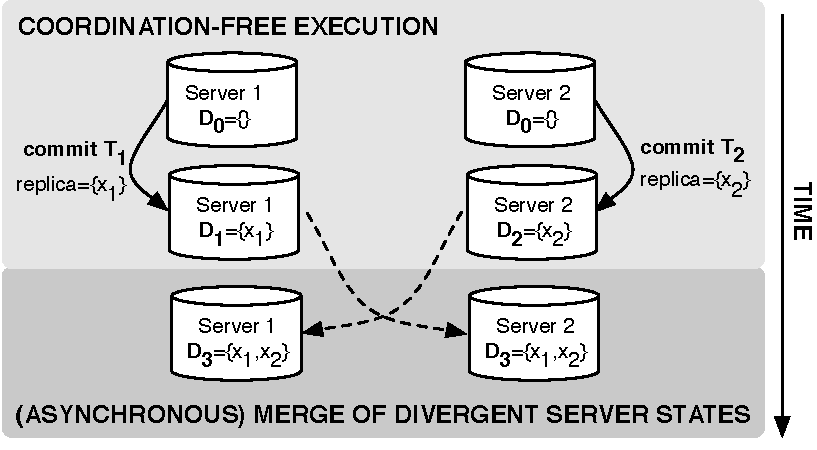
\includegraphics[width=\figscale\columnwidth]{figs/replicas.pdf}\vspace{.5em}
\caption{An example coordination-free execution of two transactions,
  $T_1$ and $T_2$, on two servers. Each transaction writes to its
  local replica, then, after commit, the servers asynchronously
  exchange state and converge to a common state ($D_3$).}
\label{fig:replicas}
\end{figure}

\minihead{Convergence} Transactional availability allows replicas to
maintain valid state \textit{independently}, but it is vacuously
possible to maintain ``consistent'' database states by letting
replicas diverge (contain different state) forever. This guarantees
safety but not liveness~\cite{schneider-concurrent}. To force state
sharing, we adopt the following definition:

\begin{definition}
  A system is \textit{convergent} iff, for each pair of servers, in
  the absence of new writes to the servers and in the
  absence of indefinite communication delays between the servers,
  the servers eventually contain the same versions for any item
  they both store.
\end{definition}

To capture the process of reconciling divergent states, we use the
previously introduced merge operator: given two divergent server
states, we apply the merge operator to produce convergent state. We
assume the effects of merge are atomically visible: either all effects
of a merge are visible or none are. This assumption is not always
necessary but it simplifies our discussion and, as we later discuss,
is maintainable without coordination~\cite{ramp-sigmod14,hat-vldb}.

Our treatment of convergence uses a pair-wise definition (i.e., each
pair converges)~\cite{cac} rather than a system-wide definition (i.e., all nodes
converge). This is more restrictive than system-wide convergence but
allows us to make guarantees on progress despite partitions
between subsets of the servers. This also precludes the use of protocols such
as background consensus, which can stall indefinitely in the presence
of partitions. Like many of the other decisions in our model, this
too could be relaxed if system-wide convergence is sufficient.

\minihead{Maintaining validity} To make sure that both divergent and
convergent database states are valid and, therefore, that transactions
never observe invalid states, we introduce the following property:

\begin{definition}
A system is \textit{globally $I$-valid} iff all replicas always contain
$I$-valid state.
\end{definition}

\minihead{Coordination} Our system model is missing one final
constraint on coordination between concurrent transaction
execution:

\begin{definition}
  A system provides coordination-free execution for a set of
  transactions $T$ iff the progress of executing each $t\in T$ is only
  dependent on $t$'s replica's state (i.e., the versions of the items
  $t$ reads).
\end{definition}

\noindent That is, in a coordination-free execution, each
transaction's progress towards commit/abort is independent of other
operations (e.g., writes, locking, validations) being performed on
behalf of other transactions. Thus, transaction execution cannot rely
on blocking synchronization or communication with other concurrently
running transactions. This coordination-free execution corresponds to
availability under the asynchronous network model used in
distributed computing~\cite{gilbert-cap}: progress is guaranteed
despite the possibility of indefinite delays between servers.


\minihead{A note on partial replication} We have explicitly considered
a replicated model. This was a natural in allowing us to reason about
distributed and multi-versioned databases. Our model captures both
fully replicated databases, where all data items are located on all
servers, and partially replicated databases, where data items are
located on a proper subset of servers. That is, as long as clients can
access \textit{some} copy of the data items they are looking for, they
are allowed to proceed. This allows us to reason about properties over
the entire set of data items (i.e., the abstraction of a replica is a
copy of the whole database), without having to describe data
placement. The distinction is not relevant from the perspective of
reasoning about coordination requirements: if two operations can
proceed independently, irrespective of any side-effects, timing, or
other information produced (or not) by the other, then the question of
whether the data they operate under is stored on multiple servers or
one server is irrelevant.

To illustrate this point, a coordination-free algorithm designed for a
partially replicated system will trivially execute on a fully
replicated system. A coordination-free algorithm designed for a fully
replicated system can execute on a partially replicated system by
having each client operate over its own independent set of versions
until writes quiesce. The latter is not practical but illustrates our
point. In practice, building efficient algorithms for partitioned
databases is challenging; for example, Chapter~\ref{c.ramp} is devoted
to a suite of algorithms for enforcing a common semantics in
partially-replicated databases.

However, in a partially replicated system implementation, checking
whether an invariant is satisfied over a transaction's logical replica
state prior to transaction commit may require transactions to access
servers containing data that they did not directly mention in their
program text. In effect, each transaction must end with an inline
invariant check over any data it modifies and any data referenced by
invariants over the data it modifies to avoid the transaction
committing a non-$I$-valid state. Thus, in a partially replicated
system, this checking can incur communication overhead (e.g., to
ensure that the opposite end of a foreign key relation is
present)---although not always (e.g., to check for a null value upon
insertion). This cost is fundamental to general-purpose invariant
verification in partially replicated systems and has well-studied
relatives in active database
systems~\cite{aiken-confluence,activedb-book} but is---as a
consequence of our decision not to distinguish fully-replicated and
partially-replicated stores---not transparent in our model.

\minihead{A note on convergence} We have chosen to implement
convergence using anti-entropy~\cite{antientropy,optimistic} via the
merge operator. In our model, servers exchange versions by shipping
the \textit{side effects} of transactions rather than the transactions
themselves. Alternatives, such as shipping closures containing the
transactions~\cite{bayou} are possible but are less common in
practice~\cite{queue,dynamo}. Our goal here is that, under a merge
function like set union, transaction effects are propagated, and
transactions are not ``rewritten'' as in alternative extended
transaction models such as compensating actions
(Chapter~\ref{c.relatedwork}).

\minihead{Alternative Merges} As discussed above, merge need not
necessarily be associative, commutative, and idempotent. For example,
in Bayou~\cite{bayou}, users write arbitrary merge functions (that may
not be commutative, associative, or idempotent) and the server
processes determine a total ordering on merge operations in the
background. As long as there is eventually connectivity between all
servers, Bayou guarantees convergence. Thus, the system is convergent
insofar as all servers replay all relevant merge operations even
though the merges themselves are not. Nevertheless, due to their
practical implementation, we focus on associative, commutative, and
idempotent merges here.

\minihead{By example} Figure~\ref{fig:replicas} illustrates a
coordination-free execution of two transactions $T_1$ and $T_2$ on two
separate, fully-replicated physical servers. Each transaction commits
on its local replica, and the result of each transaction is reflected
in the transaction's local server state. After the transactions have
completed, the servers exchange state and, after applying the merge
operator, converge to the same state. Any transactions executing later on
either server will obtain a replica that includes the effects of both transactions.


\chapter{\IConfluence and Coordination}
\label{c.iconfluence}

With a system model and goals in hand, we now address the question:
when do applications require coordination for correctness? The answer
depends not just on an application's transactions or on an 
application's invariants. Rather, the answer depends on the
\textit{combination} of the two under consideration. Our contribution
in this section is to formulate a criterion that will answer this
question for specific combinations in an implementation-agnostic
manner.

In this section, we focus almost exclusively on providing a general
answer to this question. The remainder of this thesis is devoted to
practical interpretation and application of these results.

\section{\IConfluence: Criteria Defined}
\label{sec:ic-defs}

To begin, we introduce the central property (adapted from the
constraint programming literature~\cite{obs-confluence}) in our main
result: \iconfluence. Applied in a transactional context, the
\iconfluence property informally ensures that divergent but $I$-valid
database states can be merged into a valid database state---that is,
the set of valid states reachable by executing transactions and
merging their results is closed (w.r.t. validity) under merge. In the
next sub-section, we show that \iconfluence analysis directly
determines the potential for safe, \cfree execution.

We say that a database $D_i$ is a \textit{$I$-$T$-reachable state} if,
given an invariant $I$ and set of transactions $T$ (with merge
function $\sqcup$), there exists a partially ordered set of
transaction and merge function invocations that yields $D_i$, and each
intermediate state produced by transaction execution or merge
invocation is also $I$-valid. We call these previous states
\textit{ancestor states}. Each ancestor state is either the
initial state $D_0$ or is $I$-$T$-reachable from $D_0$.

We can now formalize the \iconfluence property:

\begin{definition}[\IConfluence]
  A set of transactions $T$ is \iconfluent with respect to invariant
  $I$ if, for all $I$-$T$-reachable states $D_i$, $D_j$ with a common
  ancestor state, $D_i \sqcup D_j$ is $I$-valid.
\end{definition}

Figure~\ref{fig:iconfluence} depicts a \iconfluent merge of
two $I$-$T$-reachable states, each starting from a shared,
$I$-$T$-reachable state $D_s$. Two sequences of transactions
$t_{in}\dots t_{i1}$ and $t_{jm}\dots t_{j1}$ each independently
modify $D_s$. Under \iconfluence, the states produced by these
sequences ($D_{in}$ and $D_{jm}$) must be valid under
merge.

We require our merged states in the \iconfluence formulation to have a
common ancestor to rule out the possibility of merging states that
could not have arisen from transaction execution (e.g., even if no
transaction assigns IDs, merging two states that each have unique but
overlapping sets of IDs could be invalid). Moreover, in practice,
every non-\iconfluent set of transactions and invariants we
encountered had a counter-example execution consisting of a divergent
execution consisting of a single pair of transactions. However, we
admit the possiblity that more exotic transactions and merge functions
might lead to complex behavior in non-single-step divergence, so we
consider arbitrary histories here. Precisely characterizing the
difference in expressive power between \iconfluent transactions under
single-transaction divergence versus multi-transaction divergence is
an interesting question for future work.

\Iconfluence holds for specific combinations of invariants and
transactions. In our payroll database example from
Section~\ref{sec:t-motivation}, removing a user from the database is
\iconfluent with respect to the invariant that user IDs are
unique. However, two transactions that remove two different users from
the database are not \iconfluent with respect to the invariant that
there exists at least one user in the database at all times. Later
chapters discuss actual combinations of transactions and invariants
(and with greater precision).

\begin{figure}
\begin{center}
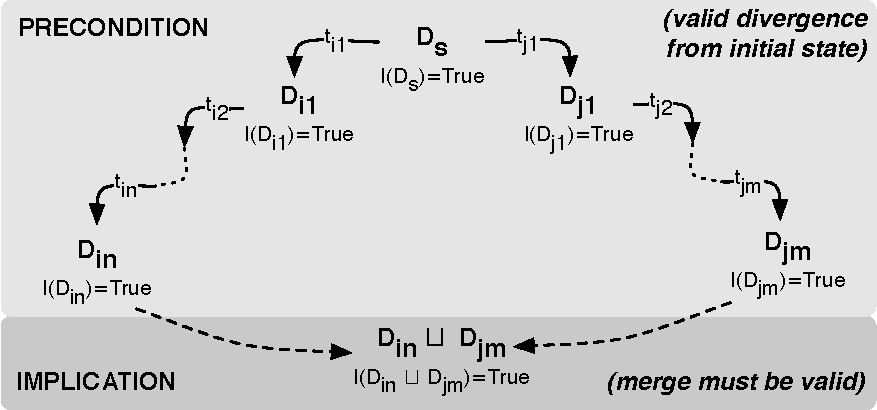
\includegraphics[width=\figscale\columnwidth]{figs/icommute.pdf}\vspace{-1em}
\end{center}\vspace{1em}
\caption{A \iconfluent execution illustrated via a diamond
  diagram. If a set of transactions $T$ is \iconfluent, then all
  database states reachable by executing and merging transactions in
  $T$ starting with a common ancestor ($D_s$) must
  be mergeable ($\sqcup$) into an $I$-valid database state.}
\label{fig:iconfluence}
\end{figure}

\section{\IConfluence and Coordination-Freedom}
\label{sec:ic-result}

We now apply \iconfluence to our goals from Section~\ref{sec:model}:

\begin{theorem}
\label{theorem:necessary}
A globally $I$-valid system can execute a set of transactions $T$ with
\cfreedom, transactional availability, and convergence if and only if $T$
is \iconfluent with respect to $I$.
\end{theorem}

Theorem~\ref{theorem:necessary} establishes \iconfluence as a
necessary and sufficient condition for invariant-preserving,
coordination-free execution.  If \iconfluence holds, there exists a
correct, coordination-free execution strategy for the transactions; if
not, no possible implementation can guarantee these properties for the
provided invariants and transactions. That is, if \iconfluence does
not hold, there exists at least one execution of transactions on
separate replicas that will violate the given invariants when servers
converge. To prevent invalid states from occurring, at least one of
the transaction sequences will have to forego availability or
\cfreedom, or the system will have to forego convergence. \Iconfluence
analysis is independent of any given implementation, and effectively
``lifts'' prior discussions of scalability, availability, and low
latency~\cite{hat-vldb,gilbert-cap,pacelc} to the level of application
(i.e., not ``I/O''~\cite{consistency-borders}) correctness. This
provides a useful handle on the implications of coordination-free
execution without requiring reasoning about low-level properties such
as physical data location and the number of servers.

We provide a full proof of Theorem~\ref{theorem:necessary} below but
first provide a sketch. The backward direction is by construction: if
\iconfluence holds, each replica can check each transaction's
modifications locally and replicas can merge independent modifications
to guarantee convergence to a valid state. The forwards direction uses
a partitioning argument~\cite{gilbert-cap} to derive a contradiction:
we construct a scenario under which a system cannot determine whether
a non-\iconfluent transaction should commit without violating one of
our desired properties (either compromising validity or availability,
diverging forever, or coordinating). The structure of our
argument is not novel, but the ability to discuss the effects of
operations without discussing the underlying system behavior (e.g.,
the presence of network partitions) is useful.

To begin, we demonstrate the possibility of forcing a
coordination-free system into any $I$-$T$-reachable database state via
a carefully crafted sequence of partitioning behavior.

\begin{lemma}\label{lemma:force} 
Given a set of transactions $T$ and invariants $I$, a globally $I$-valid, coordination-free, transactionally available, and convergent system is able to produce any $I$-$T$-reachable state $S_i$.
 \end{lemma}

\begin{proof}[Proof Lemma~\ref{lemma:force}]
Let $\alpha_i$ represent a partially ordered sequence of transactions $T_i$ and merge procedure invocations $M_i$ (call this a \textit{history}) starting from $S_0$ that produces $S_i$.

We $\textsc{replay}$ the history $\alpha$ on a set of servers as
follows. Starting from the initial state $S_0$, we traverse the
partial order according to a topological sort. Initially, we mark all
operations (transactions or merges) in $\alpha$ as \textit{not
  done}. We begin by executing all transactions $T_i$ in $\alpha_i$
that have no predeceding operations in $\alpha$. For each transaction
$t \in T_i$, we execute $t$ on a server that is unable to communicate
with any other server.\footnote{Without loss of generality, we discuss
  replicated databases, where each server contains the entire set of
  items referenced in the history. It is trivial to extend the
  \textsc{replay} procedure to a partially replicated environment by
  replacing each server with a set of servers that contains all data
  items necessary for each operation.} Upon transaction commit, we
merge each replica's modifications into the server.  (Recall that,
because $S_i$ is $I$-$T$-reachable, each transaction in $\alpha$ is an
$I$-valid transformation and must either eventually commit or abort
itself to preserve transactional availability, and, due to
coordination-freedom, the result of the execution is dependent solely
on its input---in this case, $S_0$.) We subsequently mark each
executed transaction $t$ as \textit{done} and denote the server that
executed $t$ as $s_t$.\footnote{Recall from Section~\ref{sec:model}
  that we consider arbitrary groups of servers. Thus, we simply
  execute each operation in the history on a new server. We could be
  more parsimonious with our use of servers in this procedure but
  choose not to do so for simplicity.}

Next, we repeatedly select an operation $o_i$ from $\alpha$ that is
marked as \textit{not done} but whose preceding operations are all
marked as \textit{done}.

If $o_i$ is a transaction with preceding operation $o_j$, performed
corresponding server $s_j$, we \textit{partition} $s_j$, and a second
server $s_i$, a server containing state $S_0$, such that $s_j$ and
$s_i$ can communicate with each other but cannot communicate with any
other server. Under convergent execution, $s_j$ and $s_i$ must
eventually contain the same state (given that $s_j \sqcup S_0$ is
defined in our model to be $s_j$). Following convergence, we partition
$s_j$ and $s_i$ so they can no longer communicate.\footnote{In the
  event that $o_i$ is the only event that immediately follows $o_j$ in
  $\alpha$, we could simply execute $o_i$ on $s_j$. In the event that
  multiple operations immediately follow $o_j$ in $\alpha$, we need to
  ensure that each operation proceeds independently. Thus, we are
  conservative and give every operation its own server that contains
  the effects of the preceding operations in $\alpha$.} We
subsequently execute $o_i$ on $s_i$. Again, $o_i$ must either commit
or abort itself to preserve transactional availability, and its
behavior is solely dependent on its input due to
coordination-freedom. Once $o_i$ is completed, we mark it as
\textit{done}.

If $o_i$ is a merge procedure with preceding operations $o_j$ and
$o_k$ on corresponding servers $s_j$ and $s_k$, we produce servers
$s_{j'}$ and $s_{k'}$ containing the same contents as $s_j$ and $s_k$,
respectively, as above, by partitioning $s_{j'}$ and $s_{j}$ and,
respectively, $s_{k}$ and $s_{k'}$, waiting until convergence, then
repartitioning each. Subsequently, we place $s_{j'}$ and $s_{k'}$ in
the same network partition, forcing the merge ($o_i$) of these states
via the convergence requirement. We subsequently mark $o_i$ as
\textit{done}.

When all operations in $\alpha$ are marked as \textit{done}, the
final operation we have performed will produce server containing state
$S_i$. We have effectively (serially) traversed the history, inducing
the partially ordered sequence of transactions and merges by
triggering partitions; we force transaction commits due to
transactional availability and merges due to our pair-wise
convergence requirement.
\end{proof}

Given this possibility, we proceed to prove
Theorem~\ref{theorem:necessary} from Section~\ref{sec:ic-result}.

\begin{proof}[Proof Theorem~\ref{theorem:necessary}]
($\Leftarrow$) We begin with the simpler proof, which is by
  construction. Assume a set of transactions $T$ are \iconfluent with
  respect to an invariant $I$. Consider a system in which each server
  executes the transactions it receives against a replica of its current state and checks whether or not the resulting state is $I$-valid. If
  the resulting state is $I$-valid, the replica commits the
  transaction and its mutations to the state. If not, the replica
  aborts the transaction. Servers opportunistically exchange copies of
  their local states and merge them. No individual replica will
  install an invalid state upon executing transactions, and, because
  $T$ is \iconfluent under $I$, the merge of any two $I$-valid replica
  states from individual servers (i.e., $I$-$T$-reachable states) as
  constructed above is $I$-valid. Therefore, the converged database
  state will be $I$-valid. Transactional availability, convergence,
  and global $I$-validity are all maintained via coordination-free
  execution.

  ($\Rightarrow$) Assume a system $M$ guarantees globally $I$-valid
  operation for set of transactions $T$ and invariant $I$ with
  \cfreedom, transactional availability, and convergence, but $T$ is
  not $I$-confluent. Then there exist two $I$-$T$-reachable states
  $S_a$ and $S_b$ with common ancestor $I$-$T$-reachable state $S_o$
  such that, by definition, $I(S_a)$ and $I(S_b)$ are true, but $I(S_a
  \sqcup S_b)$ is false. Call the history that corresponds to $S_a$
  $\alpha_a$ and the thisory that corresponds to $S_b$
  $\alpha_b$.\footnote{We may be able to apply Newman's lemma and only
    consider single-transaction divergence (in the case of convergent
    and therefore ``terminating''
    executions)~\cite{obs-confluence,termrewriting}, but this is not
    necessary for our results.\label{fn:newman-note}}

  Consider two executions of system $M$ corresponding to histories
  $\alpha_a$ and $\alpha_b$. In each execution, we begin by forcing
  $M$ to produce a server containing $S_o$ (via invoking
  \textsc{replay} from Lemma~\ref{lemma:force} on $M$). In $\alpha_a$, we subsequently
  \textsc{replay} the history from $S_o$ using $M$. In $\alpha_b$, we
  subsequently \textsc{replay} the history $\alpha_b$ starting from
  $S_c$. Call $T_{fa}$ and $T_{fb}$ the final (set of) transactions
  that produced each of $S_a$ and $S_b$ (that is, the set of
  transactions in each execution that are not followed by any other
  transaction). During the execution of $\alpha_a$ and $\alpha_b$, all
  transactions in each of $T_{fa}$ and $T_{fb}$ will have committed to
  maintain transactional availability, their end result will be
  equivalent to the result in $S_a$ and $S_b$, which are both
  $I$-valid, by assumption.

  We now consider a third execution, $\alpha_c$. $\alpha_c$ produces a
  server containing $S_o$ by performing \textsc{replay} using $M$, as
  above. Then, $\alpha_c$ independently performs \textsc{replay}
  for $\alpha_a$ and $\alpha_b$ but does not execute or
  proceed further in either history than the first element of $T_{fa}$
  or $T_{fb}$. Instead, we consider these specially:

  First, note that, if we independently \textsc{replay} the
  transactions in $T_{fa}$ and $T_{fb}$, and $M$ commits them, then we
  will have completed all operations in $\alpha_a$ and $\alpha_b$. In
  this case, $M$ will produce two servers $s_a$ and $s_b$ containing
  states $S_a$ and $S_b$. If we partition servers $s_a$ and $s_b$ such
  that they can communicate with each other but cannot communicate
  with any other servers, $s_i$ and $s_j$ must eventually
  converge. When $s_a$ and $s_b$ eventually converge, they will
  converge to $S_a \sqcup S_b$. However, $I(S_a \sqcup S_b)$ is false,
  which would violate global $I$-validity. Thus, $M$ cannot commit all
  of the transactions in $T_{fa}$ and $T_{fb}$.

  On the other hand, suppose we independently \textsc{replay} the the
  transactions in $T_{fa}$ and $T_{fb}$ and $M$ aborts one of the
  transactions $t_a$ in $T_{fa}$. In this case, the server that aborts
  $t_a$ (call this server $s_{ac}$) will have exactly the same
  information (set of versions) available to it as the server that
  executed $t_a$ in the execution corresponding to $\alpha_a$ above
  (call this second server $s_{aa}$). However, in the execution
  corresponding to $\alpha_a$, $s_{aa}$ committed $t_a$. Thus, in one
  execution ($\alpha_a$), $M$ commits $t_{a}$ (on $s_{ac}$) and, in another
  execution ($\alpha_c$), $M$ aborts $t_{a}$ (on $s_{aa}$), even though the
  contents of the servers are identical. Thus, despite the fact that
  the configurations are indistinguishable, $M$ performs a different
  operation, a contradiction. If we \textsc{replay} the transactions
  in $T_{fa}$ and $T_{fb}$ and $M$ aborts one of the transactions
  $t_b$ in $T_{fb}$, we will similarly observe a contradiction: a
  server in the execution corresponding to $\alpha_c$ will have aborted a
  transaction despite having the same information available to it as
  another server in the execution corresponding to $\alpha_b$, which
  committed the same transaction. Thus, to the servers executing
  $T_{fb}$, $\alpha_a$ is indistinguishable from $\alpha_c$, and, to the
  servers executing $T_{fb}$, $\alpha_b$ is indistinguishable from $\alpha_c$.

  Therefore, to preserve transactional availability in the execution
  corresponding to $\alpha_c$, $M$ must sacrifice one of global
  validity (by allowing the merge of $S_a$ and $S_b$, resulting in an
  invalid state), convergence (by never merging the contents of the
  servers containing $S_a$ and $S_b$), or \cfreedom (by requiring
  communication between servers during \textsc{replay}).
\end{proof}

\section{Discussion and Limitations}
\label{sec:theory-discussion}

\IConfluence captures a simple, informal rule:
\textbf{\textit{coordination can only be avoided if all local commit
    decisions are globally valid}}. (Alternatively, commit decisions
are composable.) If two independent decisions to commit can result in
invalid merged (converged) state, then replicas must coordinate in
order to ensure that only one of the decisions is to commit. Given the
existence of an unsafe execution and the inability to detect the
unsafe execution using only local information, a globally valid system
\textit{must} coordinate in order to prevent the invalid execution
from arising.

\minihead{Use of invariants} Our use of invariants in \iconfluence is
key to achieving a \textit{necessary} and not simply sufficient
condition. By directly capturing correctness criteria via invariants,
\iconfluence analysis only identifies ``true'' conflicts. This allows
\iconfluence analysis to perform a more accurate assessment of whether
coordination is needed compared to related conditions such as
commutativity (Chapter~\ref{c.relatedwork}).

However, the reliance on invariants also has drawbacks. \Iconfluence
analysis only guards against violations of any specified
invariants. If invariants are incorrectly or incompletely specified, a
\iconfluent database system may violate correctness. If users cannot
guarantee the correctness and completeness of their invariants and
operations, they should opt for a more conservative analysis or
mechanism such as employing serializable transactions. In fact,
without such a correctness specification, for arbitrary transaction
schedules, serializability is---in a sense---the ``optimal''
strategy~\cite{kung1979optimality}. Alternatively, restricting the
programming language---for example, to allow only \iconfluent
operations or operations that exhibit other, possibly more
conservative properties like monotonicity or commutativity
(Chapter~\ref{c.relatedwork})---can also assist here. In either case,
by casting correctness in terms of admissible application states
instead of (simply) a property of read-write executions over
distributed replicas, we achieve a more precise statement of
coordination overheads. Finally, when full application invariants are
unavailable, individual, high-value transactions may be amenable to
optimization via \iconfluence coordination analysis. Accordingly, our
development of \iconfluence analysis provides developers with a
powerful option---but only if used correctly. If used incorrectly,
\iconfluence allows incorrect results, or, if not used at all,
developers must resort to existing alternatives.

This final point raises several questions: can we specify invariants
in real-world use cases? Classic database concurrency control models
assume that ``the [set of application invariants] is generally not
known to the system but is embodied in the structure of the
transaction''~\cite{traiger-tods,eswaran-consistency}. Nevertheless,
since 1976, databases have introduced support for a finite set of
invariants~\cite{korth-serializability,decomp-semantics,garciamolina-semantics,ic-survey,ic-survey-two}
in the form of primary key, foreign key, uniqueness, and row-level
``check'' constraints~\cite{kemme-si-ic}. We can (and, in the
remainder of this dissertation, do) analyze these invariants, which
can---like many program analyses~\cite{kohler-commutativity}---lead to
new insights about execution strategies. We have found the process of
invariant specification to be non-trivial but feasible in practice. In
many cases, specifications for certain invariants already exist but have not
been examined in the context of coordination-free implementation.

\minihead{Physical and logical replication} We have used the concept
of replicas to reason about concurrent transaction execution. However,
as previously noted, our use of replicas is simply a formal device
used to capture concurrency in the system implementation, independent
of the actual concurrency control mechanisms at work. Specifically,
reasoning about replicas allows us to separate the \textit{analysis}
of transactions from their \textit{implementation}: just because a
transaction is executed with (or without) coordination does not mean
that all query plans or implementations require (or do not require)
coordination~\cite{hat-vldb}. Simply because an application is
\iconfluent does not mean that all implementations will be
coordination-free. Rather, \iconfluence ensures that a
coordination-free implementation exists.

\minihead{(Non-)determinism} \Iconfluence analysis effectively
captures points of \textit{unsafe
  non-determinism}~\cite{consistency-borders} in transaction
execution. As we have seen in many of our examples thus far, total
non-determinism under concurrent execution can compromise
application-level consistency~\cite{calm,termrewriting}. But not all
non-determinism is bad: many desirable properties (e.g., classical
distributed consensus among processes) involve forms of acceptable
non-determinism (e.g., any proposed outcome is acceptable as long as
all processes agree)~\cite{paxos-commit}. In many cases, maximizing
concurrency requires admitting the possibility of non-determinism in
outcomes.

\Iconfluence analysis allows this non-deterministic divergence of
database states but makes two useful guarantees about those
states. First, the requirement for global validity ensures safety (in
the form of invariants). Second, the requirement for convergence
ensures liveness (in the form of convergence). Accordingly, via its
use of invariants, \iconfluence allows users to scope non-determinism
while only permitting systems to produce ``acceptable'' states.

\section{Summary}

In this chapter, we developed a framework for determining whether a
given safety property can be maintained without coordination while
still guaranteeing availability of operations and convergence of
data. This \iconfluence generalizes partitioning arguments from
distributed systems and allows us to reason about semantic properties
at the application level. In effect, if the set of database states
reachable by applying program operations and merge invocations is
closed with respect to declared invariants, a coordination-free
implementation of those operations and invariants is possible. In the
remainder of this dissertation, we will
apply this \iconfluence to several semantic properties found in real
database systems.


\chapter{Coordination Avoidance and Weak Isolation}
\label{c.isolation}

In this section, we begin to apply the \iconfluence property to the
semantics found in today's database systems. We examine the
potential for coordination-free execution of transaction under a
number of \textit{weak isolation} guarantees. These non-serializable
transaction semantics are widespread use in today's database engines
and therefore provide an attractive target for \iconfluence
analysis. They are also among the lowest-level semantics we will
investigate in this thesis; that is, these guarantees pertain to the
admissible interleavings of individual reads and writes to opaque
variables, rather than whole program behavior or invariants over
database states. Thus, our primary motivation in this section is to
examine a range of widely-deployed---if not widely
understood---guarantees. Subsequently, we will move upwards in levels
of abstraction.

We provide background on the use of weak isolation in
Section~\ref{sec:modernacid}. We examine the \iconfluence of these
guarantees and provide several coordination-free implementations in
Section~\ref{sec:ic-isolation}. In Section~\ref{sec:hat-evaluation},
we experimentally evaluate their
benefits. Section~\ref{sec:hat-definitions} presents a more formal
model for these guarantees.

\section{ACID in the Wild}
\label{sec:modernacid}

Even within a single-node database, the coordination penalties
associated with serializability can be severe. In this context,
coordination manifests itself in the form of decreased concurrency,
performance degradation, multi-core scalability limitations, and,
sometimes, aborts due to deadlock or
contention~\cite{gray-isolation}. Accordingly, since the early 1970s,
database systems have offered a range of ACID properties weaker than
serializability: the host of so-called \textit{weak isolation} models
describe varying restrictions on the space of schedules that are
allowable by the system~\cite{adya, ansi-sql, ansicritique}. None of
these weak isolation models guarantees serializability, but, as we see
below, their benefits to concurrency are frequently considered by
database administrators and application developers to outweigh costs
of possible consistency anomalies that might arise from their use.

To better understand the prevalence of weak isolation, we surveyed the
default and maximum isolation guarantees provided by 18 databases,
often claiming to provide ``ACID'' or ``NewSQL''
functionality~\cite{hat-hotos}. As shown in
Table~\ref{table:existing}, only three out of 18 databases provided
serializability by default, and eight did not provide serializability
as an option at all. This is particularly surprising when we consider
the widespread deployment of many of these non-serializable databases,
like Oracle, which are known to power major businesses and product
functionality. While we have established that serializability is
unachievable in coordination-free systems, the widespread usage of these
alternative, weak models indicates that this inability may be of
limited importance to applications built upon database systems
today. If application writers and database vendors have already
decided that the benefits of weak isolation outweigh potential
application inconsistencies, then, in a coordination-free system that
that prohibits serializability, similar decisions may be tenable.

\begin{table}[t!]
\begin{center}
\begin{small}
\begin{tabular}{|l|c|c|}
\hline
Database & Default & Maximum\\\hline
Actian Ingres 10.0/10S & S & S\\
Aerospike & RC & RC\\
Akiban Persistit & SI & SI\\
Clustrix CLX 4100 & RR & RR\\
Greenplum 4.1 & RC & S \\
IBM DB2 10 for z/OS & CS & S\\
IBM Informix 11.50 & Depends & S\\
MySQL 5.6 & RR & S \\
MemSQL 1b & RC & RC\\
MS SQL Server 2012 & RC & S \\
NuoDB & CR & CR\\
Oracle 11g & RC & SI\\
Oracle Berkeley DB & S & S\\
Oracle Berkeley DB JE & RR & S\\
Postgres 9.2.2 & RC & S\\
SAP HANA & RC & SI\\
ScaleDB 1.02 & RC & RC\\
VoltDB & S & S\\
\hline
\multicolumn{3}{|p{7cm}|}{{\begin{small}{RC: read committed, RR: repeatable read, SI: snapshot isolation, S: serializability, CS: cursor stability, CR: consistent read}\end{small}}}\\\hline

\end{tabular}
\caption{Default and maximum isolation levels for ACID and NewSQL
  databases.}
\label{table:existing}
\end{small}
\end{center}
\end{table}

It has been unknown \textit{which} of these common isolation levels
can be provided with coordination-free execution. Existing algorithms
for providing weak isolation are often designed for a single-node
context and often rely on coordination-based concurrency control
mechanisms like locking or mututal exclusion. Moreover, we are not
aware of any prior literature that provides guidance as to the
relationship between weak isolation and coordination-free execution:
prior work has examined the relationship between serializability and
coordination-freedom~\cite{davidson-survey} and has studied several
variants of weak isolation~\cite{adya, ansicritique, gray-isolation}
but not weak isolation and coordination-free execution together.

\section{\IConfluence Analysis: Isolation Levels}
\label{sec:ic-isolation}

In this section, we determine the \iconfluence of a number of these
weak isolation guarantees. We also provide a treatment of several
distributed consistency models that are complementary to these
isolation guarantees. As Brewer states, ``systems and database
communities are separate but overlapping (with distinct
vocabulary)''~\cite{brewer-slides}. With this challenge in mind, we
build on existing properties and definitions from the database and
distributed systems literature, providing an informal
explanation and example for each guarantee.\footnote{For clarity, we
  call these ``distributed consistency'' guarantees ``isolation
  models'' as well.}  The database isolation guarantees require
particular care, since different DBMSs often use the same terminology
for different mechanisms and may provide additional guarantees in
addition to our implementation-agnostic definitions.  We draw largely
on Adya's dissertation~\cite{adya} and somewhat on its predecessor
work: the ANSI SQL specification~\cite{ansi-sql} and Berenson et al.'s
subsequent critique~\cite{ansicritique}.

In this section, we provide a short proof sketch of each guarantee and
provide a more comprehensive treatment in
Section~\ref{sec:hat-definitions}. For each \iconfluent guarantee, we
also offer proof-of-concept coordination-free algorithms. These are
not necessarily optimal or even efficient: the goal is to illustrate
the existence of algorithms. However, we will investigate performance
implications in Section~\ref{sec:hat-evaluation}.

\minihead{Informal model} In our examples, per Adya~\cite{adya}, we
exclusively consider read and write operations, denoting a write of
version $v_i$ with unique timestamp $i$ drawn from a totally ordered
domain (e.g., integers) to data item $d$ as $w_d(v_i)$ and a read from
data item $d$ returning $v_i$ as $r_d(v)$. We assume that all data
items have the null value, $\bot$, at database initialization, and,
unless otherwise specified, all transactions in the examples commit.

In our \iconfluence analysis, we reason about \textit{read-write
  histories} (or simply \textit{histories}: sets of transactions
consisting of read and write operations and their return values. Each
history can be represented as a graph of operations with various edges
that we describe below; thus, in our \iconfluence model, we reason
about the results of transaction executions in the database as
histories---or, in effect, traces of transaction execution. In this
section, we examine invariants over histories, and the set-oriented
nature of histories lends itself naturally to a set-oriented
merge. Compared to later analyses (e.g., those in
Chapter~\ref{c.constraints}), these are relatively straightforward,
and we keep their discussion brief.

Our use of read/write histories is somewhat awkward given our
data-centric expression of invariants. However, this model is
necessary for compatibility with existing descriptions of weak
isolation guarantees. One consolation is that this formalism
highlights the unintuitive nature of these guarantees. We study them
because they are in widespread use today, but we find them difficult
to reason about. As we move towards higher layers of abstraction in
later chapters, the higher level specifications are---in our
experience---much more intuitive and natural to reason about.

We also assume in this section that the final versions written to each
data item within a transaction are assigned the same timestamp. This
practice is standard in treatments of multi-version serializability
theory~\cite{bernstein-book} but is not actually enforced by Adya's
original model. It does not affect the generality of our
results\footnote{Namely, if we draw timestamps from an infinite
  domain, we can partition the ID space among replicas. In an
  implementation, this may require new servers joining a cluster to
  obtain a subset of the ID space from at least one existing cluster
  member. In a practical implementation, this could require a
  substantial number of bits for timestamp allocation. However, at an
  extreme, 256 bits support extreme transaction volumes.} but makes
several of them clearer.

We begin with \iconfluent guarantees and then present non-\iconfluent guarantees.

\subsection{\IConfluent Isolation Guarantees}
\label{sec:isolation}

To begin, Adya captures \textbf{Read Uncommitted} isolation as
\textit{PL-1}. In this model, writes to each object are totally
ordered, corresponding to the order in which they are installed in the
database. In a distributed database, different replicas may receive
writes to their local copies of data at different times but should
handle concurrent updates (i.e., overwrites) in accordance with the
total order for each item. \textit{PL-1} requires that writes to
different objects be ordered consistently across transactions,
prohibiting Adya's phenomenon $G0$ (also called ``Dirty
Writes''~\cite{ansicritique}). If we build a graph of transactions
with edges from one transaction to another when the former
overwrites the latter's write to the same object then, under Read
Uncommitted, the graph should not contain cycles~\cite{adya}. Consider
the following example:
\begin{align*}
T_1 &: w_x(1)~w_y(1)
\\T_2 &: w_x(2)~w_y(2)
\end{align*}
In this example, under Read Uncommitted, it is unacceptable for the
database to both order $T_1$'s $w_x(1)$ before $T_2$'s $w_x(2)$ and order
$T_2$'s $w_y(2)$ before $T_1$'s $w_y(1)$. 

Read Uncommitted is \iconfluent under read and write operations; we
provide a sketch here. The $G0$ phenomenon described above only pertains to
write operations, so we do not consider read operations. With unique
and totally ordered timestamps, $G0$ graphs are acyclic by
construction. To show this, consider any two transactions $T_i$ and
$T_j$ appearing in a $G0$ graph $G$, and the final versions of each
item produced by $T_i$ (timestamped $k$) and the final versions of
each item produced by $T_j$ (timestamped $l$, either $k < l$ or $l <
k$. In either case, $G$ is acyclic. Merging two acyclic graphs does
not produce new transactions, and all transactions within the two
graphs will similarly be totally ordered.

Because Read Uncommitted is \iconfluent, we can find a
coordination-free implementation. (However, note that traditional
implementations such as the lock-based implementation due to Gray in
the original formulation of Read Uncommitted~\cite{gray-isolation}),
do require coordinate.) Read Uncommitted is easily achieved by marking
each of a transaction's writes with the same timestamp (unique across
transactions; e.g., combining a client's ID with a sequence number)
and applying a ``last writer wins'' conflict reconciliation policy at
each replica. Later properties will strengthen Read Uncommitted.

\textbf{Read Committed} isolation is particularly important in
practice as it is the default isolation level of many DBMSs
(Section~\ref{sec:modernacid}). Centralized implementations differ,
with some based on long-duration exclusive locks and short-duration
read locks~\cite{gray-isolation} and others based on multiple
versions. These implementations often provide properties beyond what
is implied by the name ``Read Committed'' and what is captured by the
implementation-agnostic definition. However, under the
implementation-independent definition of Read Committed, transactions
should not access uncommitted or intermediate (i.e., non-final)
versions of data items. This prohibits both ``Dirty Writes'', as
above, and also ``Dirty Reads'' phenomena.  This isolation is Adya's
\textit{PL-2} and is formalized by prohibiting Adya's
\textit{G1\{a-c\}} (or ANSI's $P1$, or ``broad'' $P1$ [2.2] from
Berenson et al.). For instance, in the example below, $T_3$ should
never read $a=1$, and, if $T_2$ aborts, $T_3$ should not read $a=3$:
\begin{align*}
T_1 &: w_x(1)~w_x(2)
\\T_2 &: w_x(3)\\
T_3 &: r_x(a)
\end{align*}

Read Committed is also \iconfluent for read and write operations. The
basic idea is relatively straightforward: if two histories do not
contain reads of uncommitted or intermediate versions of data items,
unioning them will not introduce additional reads of uncommitted or
intermediate versions, nor will unioning them change any of the values
of that any of the reads returned (preventing $G1a$ and $G1b$). Adya's
$G1c$ is prevented by the fact that $G0$ graphs are acyclic for writes
(as above) and transactions can only read-depend on other transactions
that appear in their histories; thus, unioning two histories that do
not exhibit $G1c$ cannot introduce new edges to incur $G1c$.

Because Read Committed is \iconfluent, we can find a coordination-free
implementation: if no client ever writes uncommitted data to shared
copies of data, then transactions will never read each others' dirty
data. As a simple solution, clients can buffer their writes until they
commit, or, alternatively, can send them to servers, who will not
deliver their value to other readers until notified that the writes
have been committed. Unlike a lock-based implementation, this
implementation does not guarantee that readers observe the most recent
write to a data item, but it the implementation-agnostic definition.

Several different properties have been labeled \textbf{Repeatable
  Read} isolation. As we will show in
Section~\ref{sec:unachievable-acid}, some of these are not achievable
in a coordination-free system. However, the ANSI-standard,
implementation-agnostic definition~\cite{ansi-sql} \textit{is}
achievable and directly captures the spirit of the term: if a
transaction reads the same data more than once, it sees the same value each
time (preventing ``Fuzzy Read,'' or $P2$). In this paper, to
disambiguate between other definitions of ``Repeatable Read,'' we will
call this property ``cut isolation,'' since each transaction reads
from a non-changing cut, or snapshot, over the data items. If this
property holds over reads from a set of individual data items, we call it
\textbf{Item Cut Isolation}, and, if we also expect a cut over
predicate-based reads (e.g., \texttt{SELECT WHERE}; preventing
Phantoms~\cite{gray-isolation}, or Berenson et al.'s $P3/A3$), we have
the stronger property of \textbf{Predicate Cut-Isolation}. In the
example below, under both levels of cut isolation, $T_3$ must read
$a=1$:
\begin{align*}
\small
T_1 &: w_x(1)
\\T_2 &: w_x(2)
\\T_3 &: r_x(1)~r_x(a)
\end{align*}

Item Cut Isolation is \iconfluent for reasoning similar to Read
Committed: if two histories are valid under Item Cut Isolation,
unioning them will not change the return values of reads.

Because Item Cut Isolation is \iconfluent, we can find a
coordination-free implementation: we can have transactions store a
copy of any read data at the client such that the value that they
read for each item never changes unless they overwrite it
themselves. These stored values can be discarded at the end of each
transaction and can alternatively be accomplished on servers via
multi-versioning. Predicate Cut Isolation is also achievable in
coordination-free systems via similar caching middleware or
multi-versioning that tracks entire logical ranges of predicates in
addition to item based reads.

\subsubsection{ACID Atomicity Guarantees}
\label{sec:ta}

Atomicity, informally guaranteeing that either all or none of
transactions' effects should succeed, is core to ACID
guarantees. Although, at least by the ACID acronym, atomicity is not
an ``isolation'' property, atomicity properties also restrict the
updates visible to other transactions. Accordingly, here, we consider
the \textit{isolation} effects of atomicity, which we call
\textbf{Monotonic Atomic View (MAV)} isolation.  Under MAV, once some
of the effects of a transaction $T_i$ are observed by another
transaction $T_j$, thereafter, all effects of $T_i$ are observed by
$T_j$. That is, if a transaction $T_j$ reads a version of an object
that transaction $T_i$ wrote, then a later read by $T_j$ cannot return
a value whose later version is installed by $T_i$. Together with item
cut isolation, MAV prevents Read Skew anomalies (Berenson et al.'s
A5A) and is useful in several contexts such as maintaining foreign key
constraints, consistent global secondary indexing, and maintenance of
derived data. In the example below, under MAV, because $T_2$ has read
$T_1$'s write to $y$, $T_2$ must observe $b=c=1$ (or later versions
for each key):
\begin{align*}
\small
T_1 &: w_x(1)~w_y(1)~w_z(1)
\\T_2 &: r_x(a)~r_y(1)~r_x(b)~r_z(c)~\\[-1.5em]
\end{align*}
$T_2$ can also observe $a=\bot$, $a=1$, or a later version of $x$. In
the hierarchy of existing isolation properties, we place MAV below
Adya's \textit{PL-2L} (as it does not necessarily enforce transitive
read-write dependencies) but above Read Committed ($PL-2$). Notably,
MAV requires disallows reading intermediate writes (Adya's $G1b$):
observing all effects of a transaction implicitly requires observing
the final (committed) effects of the transaction as well.

Perplexingly, discussions of MAV are absent from existing treatments of
weak isolation. This is perhaps again due to the single-node context
in which prior work was developed: on a single server (or a fully
replicated database), MAV is achievable via lightweight locking and/or
local concurrency control over data items~\cite{gstore,
  kemme-thesis}. In contrast, in a distributed environment, MAV over
arbitrary groups of non-co-located items is considerably more difficult
to achieve with coordination-free execution.

MAV is \iconfluent for read and write operations. The reasoning is
similar to Read Committed and Item Cut Isolation: if two histories
obey MAV, then their union does not change the effects of the reads in
each history, and therefore every transaction $T$ in the unioned
history reads from the same transactions in the original history in
which $T$ was originally found, and $T$ will not miss the effects of
transactions it depends upon.

Because MAV is \iconfluent, we can find a coordination-free
implementation. Due to its utility, we develop an advanced set of
implementations of MAV in Chapter~\ref{c.ramp}.


\subsubsection{Session Guarantees}

A useful class of safety guarantees refer to real-time or
client-centric ordering within a \textit{session}, ``an abstraction
for the sequence of...operations performed during the execution of an
application''~\cite{sessionguarantees}. These ``session guarantees''
have been explored in the distributed systems
literature~\cite{sessionguarantees,vogels-defs} and sometimes in the
database literature~\cite{daudjee-session}. For us, a session
describes a context that should persist between transactions: for
example, on a social networking site, all of a user's transactions
submitted between ``log in'' and ``log out'' operations might form a
session.  Session guarantees are often expressed in a
non-transactional context, and there are several ways to extend them
to transactions. Per~\cite{daudjee-session}, we examine them in terms
of ordering across transactions.

Several session guarantees can be made with coordination-free
execution. We describe them informally below:

\vspace{.5em}\noindent The \textbf{{monotonic reads}} guarantee requires that, within
a session, subsequent reads to a given object ``never return any
previous values''; reads from each item progress according to a total
order (e.g., the order from Read Uncommitted).

\vspace{.5em}\noindent The \textbf{{monotonic writes}} guarantee
requires that each session's writes become accessible to other
transactions in the order they were committed. Any order on
transactions (as in Read Uncommitted isolation) should also be
consistent with any precedence (e.g., Adya's ordering on versions of
each item) that a global oracle would observe.

\vspace{.5em}\noindent The \textbf{{writes follow reads}} guarantee requires that, if
a session observes an effect of transaction $T_1$ and subsequently
commits transaction $T_2$, then another session can only observe
effects of $T_2$ if it can also observe $T_1$'s effects (or later
values that supersede $T_1$'s); this corresponds to Lamport's
``happens-before'' relation~\cite{lamportclocks}.  Any order on
transactions should respect this transitive order.\vspace{.5em}

The above guarantees are \iconfluent for reads and writes and can be
achieved by forcing servers to wait to reveal new writes (say, by
buffering them in separate local storage) until each write's
respective dependencies are visible on all replicas. This mechanism
effectively ensures that all clients read from a globally agreed upon
lower bound on the versions written. This is coordination-free because
a client will never block due to inability to find a server with a
sufficiently up-to-date version of a data item. However, it does not
imply that transactions within a session will observe previous updates
within the session or, in the presence of partitions, make forward
progress through the version history. The problem is that under our
standard definition of transactional availability, a system must
handle the possibility that, under a partition, an unfortunate client
will be forced to issue its next requests against a partitioned,
out-of-date server.

\subsection{Sticky Availability}

To address the above concern, we can introduce
the concept of ``stickiness'': clients can ensure continuity between
operations (e.g., reading their prior updates to a data item) by
maintaining affinity or ``stickiness'' with a server or set of
servers~\cite{vogels-defs}. In a fully replicated system, where all
servers are replicas for all data items, stickiness is simple: a
client can maintain stickiness by contacting the same server for each
of its requests. However, to stay ``sticky'' in a partially-replicated
system, where servers are replicas for subsets of the set of data
items (which we consider in this paper), a client must maintain
stickiness with a single \textit{logical} copy of the database, which
may consist of multiple physical servers. We say that a system
provides \textbf{sticky availability} if, whenever a client's
transactions is executed against a copy of database state that
reflects all of the client's prior operations, it eventually receives
a response, even in the presence of indefinitely long partitions
(where ``reflects'' is dependent on semantics). A client may choose to
become sticky available by acting as a server itself; for example, a
client might cache its reads and writes~\cite{bolton,
  sessionguarantees, swift}. Any guarantee achievable in a
coordination-free system is achievable in a sticky coordination-free
system but not vice-versa.  In the above example, if the client
remains sticky with the server that executed $T_1$, then the client
can read its writes. While sticky availability is implicit in prior
work, we believe this is one of the first instances where it is
discussed in detail.

Sticky availability permits three additional guarantees, which we
first define and then show are unavailable in a generic
coordination-free system:

\vspace{.5em}\noindent\textbf{{Read your writes}} requires that
whenever a session reads a given data item $d$ after writing a version
$d_i$ to it, the read returns the $d_i$ or another version $d_j$,
where $j > i$.

\vspace{.5em}\noindent\textbf{{PRAM}} (Pipelined Random Access Memory)
provides the illusion of serializing each of the operations (both
reads and writes) within each session and is the combination of
monotonic reads, monotonic writes, and read your
writes~\cite{herlihy-art}.

\vspace{.5em}\noindent\textbf{{Causal
    consistency}}~\cite{causalmemory} results from the combination of
all session guarantees~\cite{sessiontocausal} (i.e., PRAM with
writes-follow-reads) and is also referred to by Adya as \textit{PL-2L}
isolation~\cite{adya}).\vspace{.5em}

Read your writes is not achievable in a coordination-free system. Consider a client that executes the following two transactions:
\begin{align*}
\small
T_1 &: w_x(1)
\\T_2 &: r_x(a)
\end{align*}
If the client executes $T_1$ against a server that is partitioned from
the rest of the other servers, then, for transactional availability,
the server must allow $T_1$ to commit. If the same client subsequently
executes $T_2$ against the same (partitioned) server in the same
session, then it will be able to read its writes. However, if the
network topology changes and the client can only execute $T_2$ on a
different replica that is partitioned from the replica that executed
$T_1$, then the system will have to either stall indefinitely to allow
the client to read her writes (violating transactional availability)
or will have to sacrifice read your writes guarantees.

Accordingly, read your writes, and, by proxy, causal consistency and
PRAM require stickiness. Read your writes is provided by default in a
sticky system. Causality and PRAM guarantees can be accomplished with
well-known variants~\cite{causalmemory, bolton, eiger,
  sessionguarantees, swift} of the prior session guarantee algorithms
we presented earlier: only reveal new writes to clients when their
(respective, model-specific) dependencies have been revealed.

\begin{comment}
\subsubsection{Additional \IConfluent Guarantees}

In this section, we discuss two additional kinds of guarantees
that are achievable in coordination-free systems.

\vspace{0.5em}
\noindent{\textbf{Consistency}} A coordination-free system can make limited
application-level consistency guarantees. It can often execute
commutative and logically monotonic~\cite{calm} operations without the
risk of invalidating application-level integrity constraints and can
maintain limited criteria like foreign key constraints (via MAV). We do
not describe the entire space of application-level consistency
properties that are achievable (see Section~\ref{sec:relatedwork}) but
we specifically evaluate TPC-C transaction semantics with coordination-free
guarantees in Section~\ref{sec:hat-evaluation}.

\vspace{.5em}\noindent{\textbf{Convergence} Under arbitrary (but not
  infinite delays), coordination-free systems can ensure convergence, or
  \textit{eventual consistency}: in the absence of new mutations to a
  data item, all servers should eventually agree on the value for each
  item~\cite{cac, vogels-defs}. This is typically accomplished by any
  number of anti-entropy protocols, which periodically update
  neighboring servers with the latest value for each data
  item~\cite{antientropy}. Establishing a final convergent value is
  related to determining a total order on transaction updates to each
  item, as in Read Uncommitted.
\end{comment}

\subsection{Non-\IConfluent Semantics}
\label{sec:unachievable-hat}

At this point, we have considered most of the previously defined (and useful)
isolation guarantee that are available to coordination-free
systems. Before summarizing our possibility results, we will present
impossibility results, also defined in terms of previously identified
isolation anomalies. Most notably, it is impossible to prevent Lost
Update or Write Skew in a coordination-free system.

\subsubsection{Unachievable ACID Isolation}
\label{sec:unachievable-acid}

In this section, we demonstrate that preventing Lost Update and Write
Skew---and therefore providing Snapshot Isolation, Repeatable Read,
and one-copy serializability---inherently requires foregoing high
availability guarantees.

Berenson et al. define \textit{Lost Update} as when one
transaction $T1$ reads a given data item, a second transaction $T2$
updates the same data item, then $T1$ modifies the data item based on
its original read of the data item, ``missing'' or ``losing'' $T2$'s
newer update. Consider a database containing only the following
transactions:
\begin{align*}
T_1 &: r_x(a)~w_x(a+2)
\\T_2 &: w_x(2)
\end{align*}
If $T_1$ reads $a=1$ but $T_2$'s write to $x$ precedes $T_1$'s write
operation, then the database will end up with $a=3$, a state that
could not have resulted in a serial execution due to $T_2$'s
``Lost Update.''

It is impossible to prevent Lost Update in a highly available
environment. Consider two clients who submit the following $T_1$ and
$T_2$ as part of two separate histories $H_1$ and $H_2$.
\begin{align*}
T_1 &: r_x(100)~w_x(100+20=120)
\\T_2 &: r_x(100)~w_x(100+30=130)
\end{align*}
Regardless of whether $x=120$ or $x=130$ is chosen by a replica, the
database state could not have arisen from a serial execution of $H_1$
and $H_2$.\footnote{In this example, we assume that, as is standard in
  modern databases, databases accept values as they are written (i.e.,
  register semantics). However, if we replace the write operation with
  a richer semantics, like ``increment,'' we can avoid this
  issue. However, the problem persists in the general case.}  To
prevent this, either $T_1$ or $T_2$ should not have committed. Each
client's respective server might try to detect that another write
occurred, but this requires knowing the version of the latest write to
$x$. In our example, this reduces to a requirement for
linearizability, which is, via Gilbert and Lynch's proof of the CAP
Theorem, provably at odds with coordination-free
execution~\cite{gilbert-cap}.

\textbf{Write Skew} is a generalization of Lost Update to multiple
keys. It occurs when one transaction $T1$ reads a given data item $x$,
a second transaction $T2$ reads a different data item $y$, then $T1$
writes to $y$ and commits and $T2$ writes to $x$ and commits. As an
example of Write Skew, consider the following two transactions:
\begin{align*}
\small
T_1 &: r_y(0)~w_x(1)
\\T_2 &: r_x(0)~w_y(1)
\end{align*}
As Berenson et al. describe, if there was an integrity constraint
between $x$ and $y$ such that only one of $x$ or $y$ should have value
$1$ at any given time, then this write skew would violate the
constraint (which is preserved in serializable executions). Write skew
is a somewhat esoteric anomaly---for example, it does not appear in
TPC-C~\cite{snapshot-serializable}---but can result in improper
behavior in many unexpected scenarios, such as transfers from one bank
account to another~\cite{snapshot-serializable}. As a generalization
of Lost Update, Write Skew is also unavailable to coordination-free systems.

Consistent Read, Snapshot Isolation (including Parallel Snapshot
Isolation~\cite{walter}), and Cursor Stability guarantees are all
unavailable because they require preventing Lost Update phenomena.
Repeatable Read (defined by Gray~\cite{gray-isolation}, Berenson et
al.~\cite{ansicritique}, and Adya~\cite{adya}) and One-Copy
Serializability~\cite{1sr} need to prevent both Lost Update and Write
Skew. Their prevention requirements mean that these guarantees are
inherently unachievable in a coordination-free system.

\subsubsection{Unachievable Recency Guarantees}

Distributed data storage systems often make various recency guarantees
on reads of data items.  Unfortunately, an indefinitely long partition
can force an available system to violate any recency bound, so recency
bounds are not enforceable by coordination-free
systems~\cite{gilbert-cap}. One of the most famous of these guarantees
is linearizability~\cite{herlihy-art}, which states that reads will
return the last completed write to a data item. There are also several
other (weaker) variants such as safe and regular register
semantics. When applied to transactional semantics, the combination of
one-copy serializability and linearizability is called \textit{strong
  (or strict) one-copy serializability}~\cite{adya} (e.g.,
Spanner~\cite{spanner}). It is also common, particularly in systems
that allow reading from masters and slaves, to provide a guarantee
such as ``read a version that is no more than five seconds out of
date'' or similar. None of these guarantees are \iconfluent.

\subsubsection{Durability}

A client requiring that its transactions' effects survive $F$ server
faults requires that the client be able to contact at least $F+1$
non-failing replicas before committing. This affects availability and,
according to the model we have adopted, $F>1$ fault tolerance is not
achievable in an \iconfluent system. However, with minor modifications
to the model, we can ensure durability at a penalty to operation
availability. Namely, if we modify the definition of transactional
availability (Definition~\ref{def:ta}) such that a transaction
terminates if it can access at least $F+1$ servers for each item its
transaction, the remainder of our results hold for systems with at
least $F+1$ physical servers. This is a moderately subtle concept, but
an important consequence is that communication overhead associated
with ensuring durability is a function of $F$ and not of the physical
cluster size. Thus, if a cluster doubles in size from fifty to one
hundred physical servers, the overheads due to durability are
constant, whereas the overheads for, say, a majority consensus
algorithm will double (as the majority is a function of the number of
nodes).

\subsection{Summary}
\label{sec:hat-summary}

As we summarize in Table~\ref{table:hatcompared}, a wide range of
isolation levels are achievable in coordination-free systems. With sticky
availability, a system can achieve read your writes guarantees,
PRAM, and causal consistency. However, many other prominent semantics,
such as Snapshot Isolation, One-Copy Serializability, and Strong
Serializability cannot be achieved due to the inability to prevent
Lost Update and Write Skew phenomena.

We illustrate the hierarchy of \iconfluent, sticky, and non-\iconfluent
isolation models we have discussed in
Figure~\ref{fig:hatcompared}. Many models are simultaneously
achievable, but we find several particularly compelling. If we combine
all coordination-free and sticky guarantees, we have transactional,
causally consistent snapshot reads (i.e., Causal Transactional
Predicate Cut Isolation). If we combine MAV and P-CI, we have
transactional snapshot reads (see Chapter~\ref{c.ramp}). We can
achieve RC, MR, and RYW by simply sticking clients to servers. We can
also combine unavailable models---for example, an unavailable system
might provide PRAM and One-Copy
Serializability~\cite{daudjee-session}.

To the best of our knowledge, this is the first unification of
transactional isolation, distributed consistency, and session
guarantee models. Interestingly, strong one-copy serializability
subsumes all other models, while considering the (large) power set of
all compatible models (e.g., the diagram depicts 144 possible
coordination-free combinations) hints at the vast expanse of
consistency models found in the literature. This taxonomy is not
exhaustive, but we believe it lends substantial clarity to the
relationships between a large subset of the prominent ACID and
distributed consistency models.

In light the of current practice of deploying weak isolation levels
(Section~\ref{sec:modernacid}), it is perhaps surprising that so many
weak isolation levels are achievable with
coordination-freedom. Indeed, isolation levels such as Read Committed
expose and are defined in terms of end-user anomalies that could not
arise during serializable execution. However, the widespread usage of
these models suggests that, in many cases, applications can tolerate
these their associated anomalies. In turn, our results suggest
that--despite idiosyncrasies relating to concurrent updates and data
recency--coordination-free database systems can provide sufficiently
strong semantics for many applications. For non-\iconfluent semantics,
coordination-free databases may expose more anomalies (e.g.,
linearizability violations) than a single-site database (particularly
during network partitions). However, for, \iconfluent isolation
levels, users of single-site databases are subject to the same
(worst-case) application-level anomalies as a coordination-free
implementation. The necessary (indefinite) visibility penalties (i.e.,
the right side of Figure~\ref{fig:hatcompared}) and lack of support
for preventing concurrent updates (via the upper left half of
Figure~\ref{fig:hatcompared}) mean coordination-free systems are
\textit{not} well-suited for all applications (see
Section~\ref{sec:hat-evaluation}): these limitations are
fundamental. However, common practices such as ad-hoc, user-level
compensation and per-statement isolation ``upgrades'' (e.g.,
\texttt{SELECT FOR UPDATE} under weak isolation)---commonly used to
augment weak isolation---are also applicable in coordination-free
systems (although they may in turn compromise availability). That is,
if an application already selectively and explicitly opts-in to
coordination via SQL keywords like \texttt{SELECT FOR UPDATE}, a
coordination-avoiding system can similarly use these hints as a basis
for understanding when coordination is required.

 \newcommand{\lostupdate}{$^\dagger$}
 \newcommand{\rwskew}{$^\ddagger$}
 \newcommand{\linearizable}{$^\oplus$}

\begin{table}[t!]
\begin{tabular}{| c | p{6cm} | }\hline
\IConfluent & Read Uncommitted (RU), Read Committed (RC), Monotonic Atomic View
(MAV), Item Cut Isolation (I-CI), Predicate Cut Isolation (P-CI),
Writes Follow Reads (WFR), Monotonic Reads (MR), Monotonic Writes
(MW)\\\hline Sticky & Read Your Writes (RYW), PRAM, Causal\\\hline
Unavailable & Cursor Stability (CS)\lostupdate, Snapshot Isolation
(SI)\lostupdate, Repeatable Read (RR)\lostupdate\rwskew, One-Copy
Serializability (1SR)\lostupdate\rwskew, Recency\linearizable,
Safe\linearizable, Regular\linearizable, Linearizability\linearizable,
Strong 1SR\lostupdate\rwskew\linearizable \\\hline
\end{tabular}
\caption{Summary of \iconfluent, sticky, and
  non-\iconfluent models considered in this paper. Non-\iconfluent models are
  labeled by cause: preventing lost
  update\lostupdate, preventing write skew\rwskew, and requiring
  recency guarantees\linearizable.}
\label{table:hatcompared}
\end{table}

\begin{figure}[t!]
\centering
\begin{tikzpicture}[scale=0.8]
  \tikzstyle{sticky}=[rectangle,draw=blue!50,fill=blue!50,thick]
  \tikzstyle{noha}=[ellipse,draw=red!50,fill=red!50,thick, inner sep=0pt,minimum size=12pt]

  \tikzstyle{every node}=[font=\small]

 \node[draw=none,fill=none] (ici) at (2.4, 0) {I-CI};
 \node[draw=none,fill=none] (pci) at (3.5, 1.9) {P-CI};
 \node[draw=none,fill=none] (rc) at (-2.4, 1.9) {RC};
 \node[draw=none,fill=none] (ru) at (-2.4, 0) {RU};

 \node[draw=none,fill=none] (ra) at (0, 2) {MAV};

 \node[draw=none,fill=none] (mr) at (7.2, 0) {MR};
 \node[draw=none,fill=none] (mw) at (9.6, 0) {MW};
 \node[draw=none,fill=none] (wfr) at (4.8,0) {WFR};
 \node at (12.2,0) [sticky] (ryw) {RYW};

 \node[noha](recency) at (15, 0) {recency};
 \node[noha](safe) at (15, 2) {safe};
 \node[noha](regular) at (15, 4) {regular};
 \node[noha](linearizable) at (15, 6) {linearizable};
 \node at (9.6, 4) [sticky] (causal) {causal};
 \node at (9.6, 2) [sticky] (pram) {PRAM};
 \node[noha] (cs) at (-2.4, 4) {CS};
 \node[noha] (rr) at (0.4, 5.4) {RR};
 \node[noha] (si) at (3.5, 4) {SI};
 \node[noha] (1sr) at (3.5, 6.4) {1SR};
 \node[noha] (ssr) at (7.7, 7.2) {Strong-1SR};

 \draw [->, red] (recency) -- (safe);
 \draw [->, red] (safe) -- (regular);
 \draw [->, red] (regular) -- (linearizable);
 \draw [->, red] (linearizable) -- (ssr);
 \draw [->, red] (1sr) -- (ssr);
 
 \draw [->] (ru) -- (rc);
 \draw [->] (rc) -- (ra);
 \draw [->] (ici) -- (pci);

 \draw [->, blue] (mr) -- (pram);
 \draw [->, blue] (mw) -- (pram);
 \draw [->, blue] (wfr) -- (causal);
 \draw [->, blue] (ryw) -- (pram);
 \draw [->, blue] (pram) -- (causal);

 %\draw[snake=coil, segment aspect=0, segment amplitude=.75pt, segment length=2pt] (ru) -- (mr);
 %\draw[snake=coil, segment aspect=0, segment amplitude=.75pt, segment length=2pt] (rc) -- (ta);
 %\draw[snake=coil, segment aspect=0, segment amplitude=.75pt, segment length=2pt] (ici) -- (ta);
 %\draw[snake=coil, segment aspect=0, segment amplitude=.75pt, segment length=2pt] (pci) -- (ta);
 %\draw[snake=coil, segment aspect=0, segment amplitude=.75pt, segment length=2pt] (rc) -- (mr);
 %\draw[snake=coil, segment aspect=0, segment amplitude=.75pt, segment length=2pt] (pci) -- (mr);
 %\draw[snake=coil, segment aspect=0, segment amplitude=.75pt, segment length=2pt] (ici) -- (mr);
 %\draw[snake=coil, segment aspect=0, segment amplitude=.75pt, segment length=2pt] (ta) -- (ru);
 %\draw[snake=coil, blue, segment aspect=0, segment amplitude=.75pt, segment length=2pt] (ru) -- (causal);
 %\draw[snake=coil, segment aspect=0, segment amplitude=.75pt, segment length=2pt] (mr) -- (mw);
 %\draw[snake=coil, segment aspect=0, segment amplitude=.75pt, segment length=2pt] (wfr) -- (mw);
 %\draw[snake=coil, blue, segment aspect=0, segment amplitude=.75pt, segment length=2pt] (wfr) -- (ryw);

 \draw [->, red] (rc) -- (cs);
 \draw [->, red] (cs) -- (rr);
 \draw [->, red] (pci) -- (si);
 \draw [->, red] (ici) -- (rr);
 \draw [->, red] (rr) -- (1sr);
 \draw [->, red] (si) -- (1sr);
 \draw [->, red] (ra) -- (si);
 \draw [->, red] (ra) -- (rr);
 \draw [->, red] (causal) -- (linearizable);
 \draw [->, red] (ryw) -- (safe);

\end{tikzpicture}\vspace{.75em}
\label{fig:hat-order}
\caption{Partial ordering of \iconfluent, sticky (in boxes), and
  non-\iconfluent models (circled) from
  Table~\protect\ref{table:hatcompared}. Directed edges represent
  ordering by model strength. Incomparable models can be
  simultaneously achieved, and the availability of a combination of
  models has the availability of the least available individual
  model.}
\label{fig:hatcompared}
\end{figure}


% MAV can be achieved via multi-versioning. If clients attach vector
% clocks to every write (incrementing their own position for each
% transaction) and replicas store all writes via multi-versioning, then
% clients can safely determine which sets of data items to read; this
% approach is adopted by Swift~\cite{swift} and, to a lesser-extent,
% bolt-on causal consistency~\cite{bolton}. These systems also provide
% causal consistency and are subsequently sticky available (each is
% implemented via client-side caching). However, MAV is achievable
% without stickiness via an alternate algorithm: if servers wait to
% reveal writes until they are present on all replicas, clients do not
% need to be sticky.

\section{Implications: Existing Algorithms and Empirical Impact}
\label{sec:hat-evaluation}

Given our understanding of which isolation models are \iconfluent, in
this section, we analyze the implications of these results for
existing systems and study coordination-free implementations on public
cloud infrastructure. Specifically, we revisit traditional database
concurrency control with a focus on coordination costs and on
coordination-free execution. We also perform a experimental evaluation
of coordination-free versus non-coordination-free properties on public
cloud infrastructure.

\subsection{Existing Algorithms}
\label{sec:eval-existing}

While we have shown that the semantics of many database isolation
levels are achievable with coordination-freedom, many traditional
concurrency control mechanisms do not provide coordination-free
execution---even for \iconfluent isolation levels. Existing mechanisms
often presume (or are adapted from) single-server, non-partitioned
deployments or are otherwise adapted from mechanisms that enforce
serializability as a primary use case.

Most existing implementations of weak isolation are not
coordination-free. Lock-based mechanisms such as those in Gray's
original proposal~\cite{gray-isolation} do not degrade gracefully in
the presence of partial failures. (Note, however, that lock-based
protocols \textit{do} offer the benefit of recency guarantees.) While
multi-versioned storage systems allow for a variety of transactional
guarantees, few offer traditional weak isolation (e.g.,
non-``tentative update'' schemes) in this context.  Chan and Gray's
read-only transactions have item-cut isolation with causal consistency
and MAV (session \textit{PL-2L}~\cite{adya}) but are unavailable in
the presence of coordinator failure and assume serializable update
transactions~\cite{readonly}; this is similar to read-only and
write-only transactions more recently proposed by Eiger~\cite{eiger}.
Brantner's S3 database~\cite{kraska-s3} and
Bayou~\cite{sessionguarantees} can all provide variants of session
\textit{PL-2L} with coordination-free execution, but none provide this
coordination-free functionality without substantial
modification. Accordingly, it is possible to implement many guarantees
weaker than serializability---including coordination-free
semantics---and still not achieve a coordination-free
implementation. Thus, coordination-free execution must often be
explicitly considered in concurrency control designs.

\subsection{Empirical Impact: Isolation Guarantees}
\label{sec:prototype}

To investigate the performance implications of coordination-free weak
isolation implementation in a real-world environment, we implemented a
database prototype of several of the guarantees in this chapter. We
verify that, as Chapter~\ref{c.background}'s measurements suggested,
``strongly consistent'' algorithms incur substantial latency penalties
(over WAN, 10 to 100 times higher than their coordination-free
counterparts) compared to coordination-free-compliant algorithms,
which scale linearly. Our goal is \textit{not} a complete performance
analysis of coordination-free semantics but instead a demonstration of
coordination-free designs on real-world infrastructure.

\vspace{.5em}\noindent\textit{Implementation.} Our prototype database
is a partially replicated (hash-based partitioned) key-value backed by
LevelDB and implemented in Java using Apache Thrift. It supports
eventual consistency (hereafter, \texttt{eventual}) using a
last-writer-wins reconciliation policy for concurrent writes,
effectively providing Read Uncommitted replication, via standard
all-to-all anti-entropy between replicas. We support
non-coordination-free operation whereby all operations for a given key
are routed to a (randomly) designated \texttt{master} replica for each
key (guaranteeing single-key linearizability, as in Gilbert and
Lynch's CAP Theorem proof~\cite{gilbert-cap} and in
PNUTS~\cite{pnuts}'s ``read latest'' operation; hereafter,
\texttt{master}) as well as distributed two-phase locking. Servers are
durable: they synchronously write to LevelDB before responding to
client requests.

\vspace{.5em}\noindent\textit{Configuration.} We deploy the database
in \textit{clusters}---disjoint sets of database servers that each
contain a single, fully replicated copy of the data---across one or
more datacenters and stick all clients within a datacenter to their
respective cluster (trivially providing read-your-writes and monotonic
reads guarantees). By default, we deploy 5 Amazon EC2
\texttt{m1.xlarge} instances (15GB RAM, with 4 cores comprising 8
``EC2 Compute Units'') as servers in each cluster. For our workload,
we link our client library to the YCSB benchmark~\cite{ycsb}, which is
well suited to LevelDB's key-value schema, grouping every eight YCSB
operations from the default workload (50\% reads, 50\% writes) to form
a transaction. We increase the number of keys in the workload from the
default 1,000 to 100,000 with uniform random key access, keeping the
default value size of $1KB$, and running YCSB for 180 seconds per
configuration.

\begin{figure}[t!]
\begin{center}

\includegraphics[width=.4\columnwidth]{figs/strategylegendthree.pdf}\vspace{-1.5em}
\begin{center}
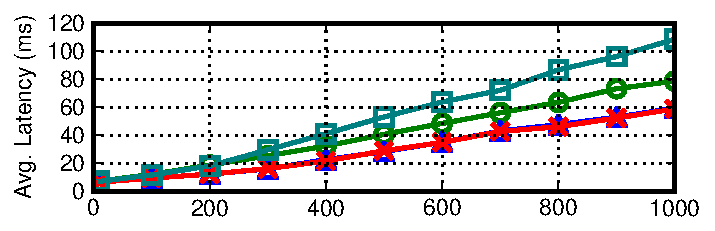
\includegraphics[width=\figscale\columnwidth]{figs/finals/2lan-threads-lats.pdf}
\vspace{-.5em}

\includegraphics[width=2.8in]{figs/hat-ycsb-label.pdf}
\begin{center}{A.) Within \texttt{us-east} \texttt{(VA)}}\end{center}
\end{center}
\begin{center}
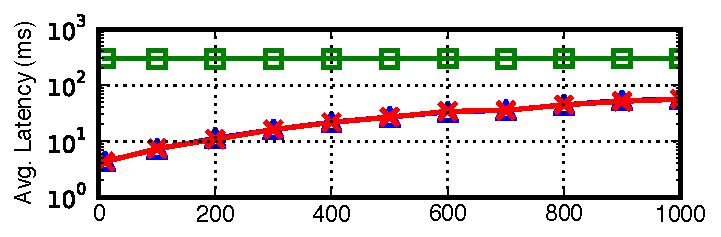
\includegraphics[width=\figscale\columnwidth]{figs/finals/2wan-threads-lats-log.pdf}\vspace{-.5em}

\includegraphics[width=2.8in]{figs/hat-ycsb-label.pdf}
\end{center}
\begin{center}{B.) Between \texttt{us-east} \texttt{(CA)} and 
    \texttt{us-west-2} \texttt{(OR)}}\end{center}\vspace{-.5em}
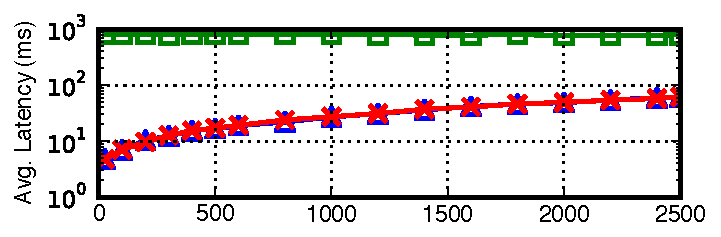
\includegraphics[width=\figscale\columnwidth]{figs/finals/5wan-threads-lats-log.pdf}\vspace{-.5em}

\includegraphics[width=2.8in]{figs/hat-ycsb-label.pdf}
\end{center}
\begin{center}{C.) Between \texttt{us-east} \texttt{(VA)}, \texttt{us-west-1} \texttt{(CA)},\\ \texttt{us-west-2} \texttt{(OR)}, \texttt{eu-west} \texttt{(IR)}, \texttt{ap-northeast} \texttt{(SI)}}\end{center}
\caption{YCSB latency for two clusters of five servers each 
  deployed within a single datacenter and cross-datacenters (note log
  scale for multi-datacenter deployment).}
\label{fig:wan-lat}
\end{figure}

\begin{figure}[t!]
\begin{center}

\includegraphics[width=.4\columnwidth]{figs/strategylegendthree.pdf}
\begin{center}{A.) Within \texttt{us-east} \texttt{(VA)}}\end{center}
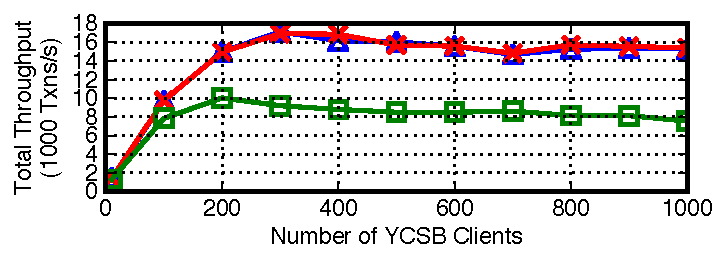
\includegraphics[width=\figscale\columnwidth]{figs/finals/2lan-threads-thru.pdf}
\begin{center}{B.) Between \texttt{us-east} \texttt{(CA)} and \texttt{us-west-2} \texttt{(OR)}}\end{center}
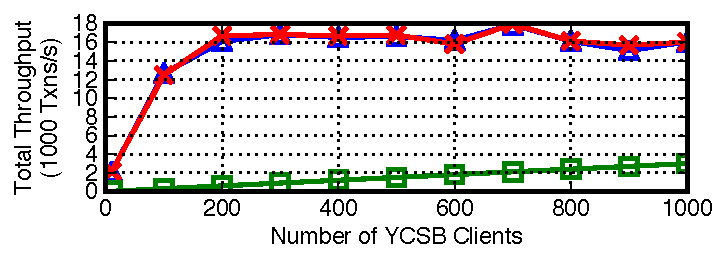
\includegraphics[width=\figscale\columnwidth]{figs/finals/2wan-threads-thru.pdf}
\begin{center}{C.) Between \texttt{us-east} \texttt{(VA)}, \texttt{us-west-1} \texttt{(CA)},\\ \texttt{us-west-2} \texttt{(OR)}, \texttt{eu-west} \texttt{(IR)}, \texttt{ap-northeast} \texttt{(SI)}}\end{center}
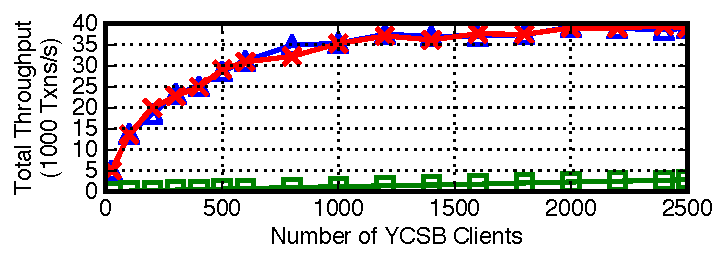
\includegraphics[width=\figscale\columnwidth]{figs/finals/5wan-threads-thru.pdf}
\end{center}
\caption{YCSB throughput for two clusters of five servers each 
  deployed within a single datacenter and cross-datacenters.}
\label{fig:wan-thru}
\end{figure}

\vspace{.5em}\noindent\textit{Geo-replication.} We first deploy the
database prototype across an increasing number of
datacenters. Figures~\ref{fig:wan-lat}A and~\ref{fig:wan-thru}A shows
that, when operating two clusters within a single datacenter,
mastering each data item results in approximately half the throughput
and double the latency of \texttt{eventual}. This is because
coordination-free models are able to utilize replicas in both clusters
instead of always contacting the (single)
master. \texttt{RC}---essentially \texttt{eventual} with
buffering---is almost identical to \texttt{eventual}. Latency
increases linearly with the number of YCSB clients.

In contrast, when the two clusters are deployed across the continental
United States (Figures~\ref{fig:wan-lat}B and~\ref{fig:wan-thru}B), the average latency of
\texttt{master} increases to $300$ms (a $278$--$4257\%$ latency
increase; average $37$ms latency per operation). For the same number
of YCSB client threads, \texttt{master} has substantially lower
throughput than the coordination-free configurations. Increasing the number of YCSB
clients \textit{does} increase the throughput of \texttt{master}, but
our Thrift-based server-side connection processing did not gracefully
handle more than several thousand concurrent connections. In contrast,
across two datacenters, the performance of eventual and RC are
near identical to a single-datacenter deployment.

\FloatBarrier

When five clusters (as opposed to two, as before) are deployed across
the five EC2 datacenters with lowest communication cost
(Figures~\ref{fig:wan-lat}C and~\ref{fig:wan-thru}C), the trend continues: \texttt{master}
latency increases to nearly $800$ms per transaction. As an attempt at
reducing this overhead, we implemented and benchmarked a variant of
quorum-based replication as in Dynamo~\cite{dynamo}, in which clients
sent requests to all replicas, which completed as soon as a majority
of servers responded (guaranteeing regular
semantics~\cite{herlihy-art}). This strategy (not pictured) did not
substantially improve performance due to the network topology and
because worst-case server load was unaffected.

Because \texttt{master} performed {far} better than our
textbook implementation, we have omitted performance data for
two-phase locking. In addition to incurring the same WAN round-trip
latency, locking also incurred substantial overheads due to mutual
exclusion. While techniques such as those recently proposed in
Calvin~\cite{calvin} can reduce the overhead of serializable
transactions by avoiding locking, our mastered implementation and the
data from Section~\ref{sec:latency} are reasonable lower bounds on
latency.

\begin{figure}[t!]

\includegraphics[width=.33\columnwidth]{figs/strategylegendtwo.pdf}\vspace{-1.5em}
\begin{center}
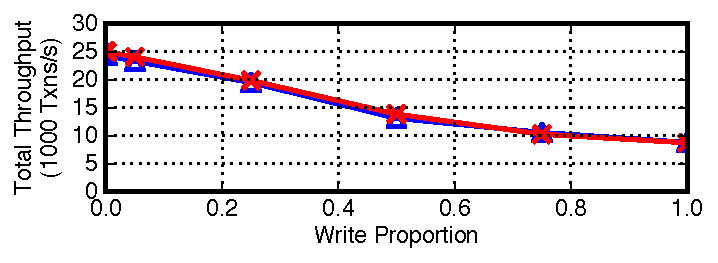
\includegraphics[width=\figscale\columnwidth]{figs/finals/wprop-thru.pdf}
\end{center}
\caption{Proportion of reads and writes versus throughput.}
\label{fig:rprop}
\begin{center}
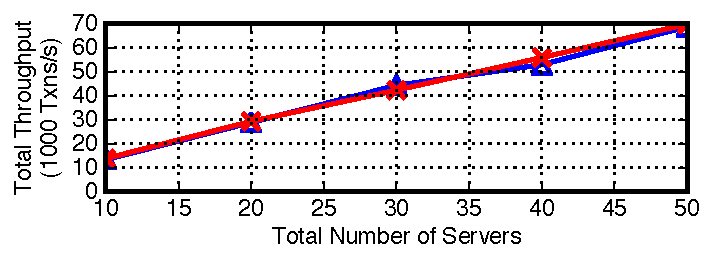
\includegraphics[width=\figscale\columnwidth]{figs/finals/scaleout-thru.pdf}
%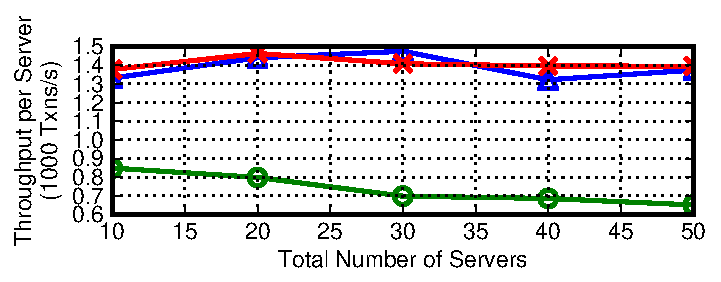
\includegraphics[width=\figscale\columnwidth]{figs/finals/scaleout-thru-perserver.pdf}
\end{center}
\caption{Scale-out of Eventual and RC.}
\label{fig:scaleout}
\end{figure}

\vspace{.5em}\noindent\textit{Read proportion.} Our default (equal)
proportion of reads and writes is fairly pessimistic: for example,
Facebook reports $99.8\%$ reads for their workload~\cite{eiger}. As
Figure~\ref{fig:rprop} demonstrates, increasing the proportion of
reads increases throughput; this is due to the decreased cost of read
operations on each node, and \texttt{RC} and \texttt{eventual} stay
matched in terms of throughput.

\vspace{.5em}\noindent\textit{Scale-out.} One of the key benefits of
our coordination-free algorithms is that they are shared-nothing~\cite{stonebraker-case}, meaning they
should not compromise scalability. Figure~\ref{fig:scaleout} shows
that varying the number of servers across two clusters in Virginia and
Oregon (with $15$ YCSB clients per server) results in linear scale-out
for \texttt{eventual} and \texttt{RC}. \texttt{RC} and
\texttt{eventual} scale linearly: increasing the number of servers per
cluster from $5$ to $25$ yields an approximately $5$x throughput
increase.

\vspace{.5em}\noindent\textit{Summary.} Our experimental prototype
confirms our earlier analytical intuition. Coordination-free systems
can provide useful semantics without substantial performance
penalties. Our coordination-free algorithms circumvent high WAN
latencies inevitable with non-coordination-free implementations. Our
results highlight Deutsch's observation that ignoring factors such as
latency can ``cause big trouble and painful learning
experiences''~\cite{fallacies-deutsch}---in a single-site context,
paying the cost of coordination may be tenable, but, especially as
services are geo-replicated, costs increase. In the next chapter, we
examine a more sophisticated set of implementations.

\FloatBarrier

\section{Isolation Models}
\label{sec:hat-definitions}

In this section, we formally define coordination-free transactional
semantics as a reference for the previous section. Our formalism is
based on that of Adya~\cite{adya}. For the reader familiar with his
formalism, this is a mostly-straightforward exercise combining
transactional models with distributed systems semantics. While the
novel aspects of this work largely pertain to \textit{using} these
definitions, we believe it is instructive to accompany them by
appropriate definitions as well.

To begin, we describe our model of weakly isolated transactions. This
is, with the exception of sessions, identical to that of
Adya~\cite{adya}. We omit a full duplication of his formalism here but
highlight several salient criteria. We refer the interested reader to
Adya's Ph.D. thesis, Section 3.1 (pp. 33--43).

Users submit transactions to a database system that contains a set of
objects, each of which is represented by multiple distinct
versions. Each transaction is composed of writes, which create new
versions of an object, and reads, which return a written version or
the initial version of the object. A transaction's last operation is
either \texttt{commit} or \texttt{abort}, and hence there is exactly one
invocation of either these two operations per
transaction. Transactions can either read individual items or read
based on predicates (or logical ``ranges'')      of data items.

\begin{definition}[Version set of a predicate-based operation]
When a transaction executes a read or write based on a predicate P,
the system selects a version for each tuple in P’s relations. The set
of selected versions is called the \textit{Version set} of this predicate-based
operation and is denoted by Vset(P).
\end{definition}

A history over transactions has two parts: first, a partial order of
events, comprised of several different types of edges that we describe
below, reflects the ordering of operations with respect to each
transaction, and, second, a order ($\ll$) on the committed versions of
each object. The history forms a graph, with nodes corresponding to
either transactions or operations within a transaction, and edges
constructed as we describe below.

As a departure from Adya's formalism, to capture the use of session
guarantees, we allow transactions to be grouped into sessions. We
represent sessions as a partial ordering on committed transactions
such that each transaction in the history appears in at most one
session.

\subsubsection{Framework}

To reason about isolation anomalies, we use Adya's concept of a
conflict graph, which is composed of dependencies between
transaction. The definitions in this section are directly from Adya,
with two differences. First, we expand Adya's formalism to deal
with \textit{per-item} dependencies. Second, we define session
dependencies (Definition~\ref{def:sd1}).

\begin{definition}[Change the Matches of a Predicate-Based Read]
A transaction $T_i$ changes the matches
of a predicate-based read $r_j$(P:Vset(P)) if $T_i$ installs $x_i$, $x_h$
immediately precedes $x_i$ in the version order, and $x_h$ matches
P whereas $x_i$ does not or vice-versa. In this case, we also
say that $x_i$ changes the matches of the predicate-based read.
The above definition identifies $T_i$ to be a transaction where
a change occurs for the matched set of $r_j$ (P: Vset(P)).
\end{definition}

\begin{definition}[Directly item-read-depends by $x$]
$T_j$ directly item-read-depends on transaction $T_i$ if $T_i$ installs some
  object version $x_i$ and $T_j$ reads $x_i$.
\end{definition}

\begin{definition}[Directly item-read-depends]
$T_j$ directly item-read-depends on transaction $T_i$ if $T_j$
  directly item-read-depends by $x$ on $T_i$ for some data item $x$.
\end{definition}

\begin{definition}[Directly predicate-read-depends by $P$]
Transaction $T_j$ directly predicate-read-depends by $P$ on
transaction $T_i$ if $T_j$ performs an operation $r_j$(P: Vset(P)),
$x_k$ $\in$ Vset(P), $i = k$ or $x_i \ll x_k$ , and $x_i$ changes the
matches of $r_j$ (P: Vset(P)).
\end{definition}


\begin{definition}[Directly Read-Depends{~\cite[Definition 2]{adya}}]
$T_j$ directly read-depends on transaction $T_i$ if it directly
item-read-depends or directly predicate-read-depends on $T_i$.
\end{definition}

\begin{definition}[Directly predicate-read-depends]
$T_j$ directly predicate-read-depends on $T_i$ if $T_j$ directly
  predicate-read-depends by $P$ on $T_i$ for some predicate $P$.
\end{definition}


\begin{definition}[Directly item-anti-depends by $x$]
$T_j$ directly item-anti-depends by $x$ on transaction $T_i$ if $T_i$
  reads some object version $x_k$ and $T_j$ installs $x$'s next
  version (after $x_k$) in the version order. Note that the
  transaction that wrote the later version directly item-anti-depends
  on the transaction that read the earlier version.
\end{definition}

\begin{definition}[Directly item-anti-depends]
$T_j$ directly item-anti-depends on transaction $T_i$ if $T_j$
  directly item-anti-depends on transaction $T_i$.
\end{definition}

\begin{definition}[Directly predicate-anti-depends by $P$]
$T_j$ directly predicate-anti-depends by $P$ on transaction $T_i$ if
  $T_j$ overwrites an operation $r_i(P:$ Vset(P)). That is, if $T_j$
  installs a later version of some object that changes the matches of
  a predicate based read performed by $T_i$.
\end{definition}

\begin{definition}[Directly Anti-Depends{~\cite[Definition 4]{adya}}]
Transaction $T_j$ directly anti-depends on transaction $T_i$ if it
directly item-anti-depends or directly predicate-anti-depends on
$T_i$.
\end{definition}

\begin{definition}[Directly Write-Depends by $x$]
A transaction $T_j$ directly write-depends by $x$ on transaction $T_i$
if $T_i$ installs a version $x_i$ and $T_j$ installs $x$'s next
version (after $x_i$) in the version order.
\end{definition}

\begin{definition}[Directly Write-Depends{~\cite[Definition 5]{adya}}]
A transaction $T_j$ directly write-depends on transaction $T_i$ if
$T_i$ directly write-depends by $x$ on $T_j$ for some item $x$.
\end{definition}

\begin{definition}[Session-Depends]
\label{def:sd1}
A transaction $T_j$ session-depends on transaction $T_i$ if $T_i$ and
$T_j$ occur in the same session and $T_i$ precedes $T_j$ in the
session commit order.
\end{definition}

The dependencies for a history $H$ form a graph called its Directed
Serialization Graph ($DSG(H)$). If $T_j$ directly write-depends on
$T_i$ by $x$, we draw $T_i\overset{ww_x}\longrightarrow T_j$. If $T_j$
read-depends on $T_i$ by $x$, we draw
$T_i \overset{wr_x}\longrightarrow T_j$. If $T_j$ directly
anti-depends on transaction $T_j$ by $x$, we draw
$T_i \overset{rw_x}\DashedArrow T_j$. If $T_j$ session-depends on
$T_i$ in session $S$, we draw $T_i \overset{S}\longrightarrow
T_j$~\cite[Definition 8]{adya}.

We also consider the Unfolded Serialization Graph ($USG(H)$) that is a
variation of the $DSG$. The USG is specified for the transaction of
interest, $T_i$, and a history, $H$, and is denoted by $USG(H,
T_i)$. For the USG, we retain all nodes and edges of the $DSG$ except
for $T_i$ and the edges incident on it. Instead, we split the node for
$T_i$ into multiple nodes---one node for every read/write event in
$T_i$. The edges are now incident on the corresponding operation of of
$T_i$.

$USG(H, T_i)$ is obtained by transforming $DSG(H)$ as follows:.  For
each node $p$ ($p \neq T_i$) in $DSG(H)$, we add a node to
$USG(H,T_i)$. For each edge from node $p$ to node $q$ in $DSG(H)$,
where p and q are different from $T_i$, we draw a corresponding edge
in $USG(H,T_i)$. Now we add a node corresponding to every read and
write performed by $T_i$. Any edge that was incident on $T_i$ in the
$DSG$ is now incident on the corresponding read or write operation on
$T_i$ in the $USG$. Finally, consecutive events in $T_i$ are connected
by \textit{order edges}, e.g., if an action (e.g., SQL statement)
reads object $y_j$ and immediately follows a write on object $x$ in
transaction $T_i$, we add an order-edge from $w_i(x_i)$ to
$r_i(y_j)$~\cite[Section 4.2.1]{adya}. Note that creating a graph
with ``supernodes'' replacing each set of read and write operations
for each $T_i$ in $USG(H)$ yields $DSG(H)$.

\subsubsection{Transactional Anomalies and Isolation Levels}
\label{sec:anomalies-hat}

Following Adya, we define isolation levels according to
possible \textit{anomalies}--typically represented by cycles in the
serialization graphs. Definitions~\ref{def:imp}--\ref{def:lostupdate}
are not found in Adya but are found (albeit not in this formalism) in
Berenson et al.~\cite{ansicritique} and the literature on session
guarantees~\cite{sessionguarantees, vogels-defs}.

\begin{definition}[Write Cycles (G0)]
A history $H$ exhibits phenomenon G0 if $DSG(H)$ contains a directed
cycle consisting entirely of write-dependency edges.
\end{definition}

\begin{definition}[Read Uncommitted]
A system that provides Read Uncommitted isolation prohibits phenomenon G0.
\end{definition}

\begin{definition}[Aborted Reads (G1a)]
A history $H$ exhibits phenomenon G1a if it contains an aborted
transaction $T_1$ and a committed transaction $T_2$ such that $T_2$ has read
some object (possibly via a predicate) modified by $T_1$.
\end{definition}

\begin{definition}[Intermediate Reads (G1b)]
  A history $H$ exhibits phenomenon G1b if it contains a committed
  transaction $T_2$ that has read a version of object $x$ (possibly
  via a predicate) written by transaction $T_1$ that was not $T_1$'s
  final modification of $x$.
\end{definition}

\begin{definition}[Circular Information Flow (G1c)]
A history $H$ exhibits phenomenon G1c if $DSG(H)$ contains a directed
cycle consisting entirely of dependency edges.
\end{definition}

\begin{definition}[Read Committed]
A system that provides Read Committed isolation prohibits phenomenon G0, G1a, G1b, and G1c.
\end{definition}

\begin{definition}[Item-Many-Preceders (IMP)]
\label{def:imp}
A history $H$ exhibits phenomenon IMP if $DSG(H)$ contains a
transaction $T_i$ such that $T_i$ directly item-read-depends by $x$ on more
than one other transaction.
\end{definition}

\begin{figure}[H]
\begin{align*}
\small
T_1 &: w_x(1)\\
T_2 &: w_x(2)\\
T_3 &: r_x(1)~r_x(2)
\end{align*}
\caption{Example of \textit{IMP} anomaly.}
\label{fig:nici-history}
\end{figure}

\begin{figure}[H]
\centering
\begin{tikzpicture}[node distance=3cm]
\tikzstyle{tx}=[draw=none, fill=none]
\node[tx] (T1) at (0,0) {$T_1$};
\node[tx] (T2) at (0,-1) {$T_2$};
\node[tx] (T3) at (2,-.5) {$T_3$};

\draw[->] (T1) edge node[above]{$wr_x$} (T3);
\draw[->] (T2) edge node[below]{$wr_x$} (T3);
\end{tikzpicture}
\caption{DSG for Figure~\ref{fig:nici-history}.}
\label{fig:nici-dsg}
\end{figure}

\begin{definition}[Item Cut Isolation (I-CI)]
A system that provides Item Cut Isolation prohibits phenomenon IMP.
\end{definition}

\begin{definition}[Predicate-Many-Preceders (PMP)]
A history $H$ exhibits phenomenon PMP if, for all predicate-based
reads $r_i(P_i:Vset(P_i))$ and $r_j(P_j:Vset(P_j)$ in $T_k$ such that
the logical ranges of $P_i$ and $P_j$ overlap (call it $P_o$), the set
of transactions that change the matches of $P_o$ for $r_i$ and $r_j$
differ.
\end{definition}

\begin{definition}[Predicate Cut Isolation (P-CI)]
A system that provides Predicate Cut Isolation prohibits phenomenon PMP.
\end{definition}

\begin{definition}[Observed Transaction Vanishes (OTV)]
\label{def:otv}
A history $H$ exhibits phenomenon OTV if $USG(H)$ contains a directed
cycle consisting of exactly one read-dependency edge by $x$ from $T_j$
to $T_i$ and a set of edges by $y$ containing at least one
anti-dependency edge from $T_i$ to $T_j$ and $T_j$'s read from $y$
precedes its read from $x$.
\end{definition}
\begin{figure}[H]
\begin{align*}
\small
T_1 &: w_x(1)~w_y(1)\\
T_2 &: w_x(2)~w_y(2)\\
T_3 &: r_x(2)~r_y(1)
\end{align*}
\caption{Example of \textit{OTV} anomaly.}
\label{fig:nta-history}
\end{figure}

\begin{figure}[H]
\centering
\begin{tikzpicture}[node distance=3cm]
\tikzstyle{tx}=[draw=none, fill=none]
\node[tx] (T1) at (0,0) {$T_1$};
\node[tx] (T2) at (2,0) {$T_2$};
\node[tx] (T3) at (2,-1.5) {$T_3$};

\draw[->] (T1) edge node[sloped, above]{$ww_{\{x, y\}}$} (T2);
\draw[->] (T1) edge [bend right] node[sloped, below]{$wr_y$} (T3);
\draw[->] (T2) edge [bend right] node[left]{$wr_x$} (T3);
\draw[dashed, ->] (T3) edge [bend right] node[right]{$rw_y$} (T2);
\end{tikzpicture}
\caption{DSG for Figure~\ref{fig:nta-history}.}
\label{fig:nta-dsg}
\end{figure}

\begin{definition}[Monotonic Atomic View (MAV)]
A system that provides Monotonic Atomic View isolation prohibits
phenomenon OTV in addition to providing Read Committed isolation.
\end{definition}

The following session guarantees are directly adapted from Terry et
al.'s original definitions~\cite{sessionguarantees}:

\begin{definition}[Non-monotonic Reads (N-MR)]
A history $H$ exhibits phenomenon N-MR if $DSG(H)$ contains a directed cycle
consisting of a transitive session-dependency between transactions
$T_j$ and $T_i$ with an anti-dependency edge by $i$ from $T_j$ and a
read-dependency edge by $i$ into $T_i$.
\end{definition}

\begin{definition}[Monotonic Reads (MR)]
A system provides Monotonic Reads if it prohibits phenomenon N-MR.
\end{definition}


\begin{figure}[H]
\begin{align*}
\small
T_1 &: w_x(1)\\
T_2 &: w_x(2)\\
T_3 &: r_x(2)\\
T_4 &: r_x(1)
\end{align*}
\caption{Example of \textit{N-MR} violation when $w_x(1) \ll w_x(2)$ and $T_4$ directly session-depends on $T_3$.}
\label{fig:nmr-history}
\end{figure}

\begin{figure}[H]
\centering
\begin{tikzpicture}[node distance=3cm]
\tikzstyle{tx}=[draw=none, fill=none]
\node[tx] (T1) at (0,0) {$T_1$};
\node[tx] (T2) at (3,0) {$T_2$};

\node[tx] (T3) at (0,-2) {$T_3$};
\node[tx] (T4) at (3,-2) {$T_4$};

\draw[->] (T1) edge node[above]{$ww_x$} (T2);
\draw[->] (T3) edge node[below]{$s_i$} (T4);

\draw[->] (T2) edge node[sloped, above]{$wr_x$} (T3);
%\draw[->] (T2) edge [bend right] node[left]{$wr_x$} (T4);
%\draw[->] (T1) edge [bend right]node[right]{$wr_x$} (T4);
\draw[dashed, ->] (T4) edge [bend right]node[right]{$rw_x$} (T2);
\end{tikzpicture}
\caption{DSG for Figure~\ref{fig:nmr-history}. $wr_x$ dependency from $T_1$ to $T_4$ omitted.} 
\label{fig:nmr-dsg}
\end{figure}

\begin{definition}[Non-monotonic Writes (N-MW)]
A history $H$ exhibits phenomenon N-MW if $DSG(H)$ contains a directed cycle
consisting of a transitive session-dependency between transactions
$T_j$ and $T_i$ and at least one write-dependency edge.
\end{definition}


\begin{figure}[H]
\begin{align*}
\small
T_1 &: w_x(1)\\
T_2 &: w_y(1)\\
T_3 &: r_y(1)~r_x(0)
\end{align*}
\caption{Example of \textit{N-MW} anomaly if $T_2$ directly session-depends on $T_1$.}
\label{fig:nmw-history}
\end{figure}

\begin{figure}[H]
\centering
\begin{tikzpicture}[node distance=3cm]
\tikzstyle{tx}=[draw=none, fill=none]
\node[tx] (T1) at (0,0) {$T_1$};
\node[tx] (T2) at (2,0) {$T_2$};
\node[tx] (T3) at (2,-1) {$T_3$};

\draw[->] (T1) edge node[above]{$s_i$} (T2);
\draw[->] (T2) edge node[right]{$wr_y$} (T3);
\draw[->, dashed] (T3) edge node[below, sloped]{$rw_x$} (T1);
\end{tikzpicture}
\caption{DSG for Figure~\ref{fig:nmw-history}.}
\label{fig:nmw-dsg}
\end{figure}


\begin{definition}[Monotonic Writes (MW)]
A system provides Monotonic Writes if it prohibits phenomenon N-MW.
\end{definition}

\begin{definition}[Missing Read-Write Dependency (MRWD)]
A history $H$ exhibits phenomenon MRWD if, in $DSG(H)$, for all
committed transactions $T_1$, $T_2$, $T_3$ such that $T_2$
read-depends on $T_1$ and $T_3$ read-depends on $T_2$, $T_3$ does
not directly anti-depend on $T_1$.
\end{definition}


\begin{figure}[H]
\begin{align*}
\small
T_1 &: w_x(1)\\
T_2 &: r_x(1)~w_y(1)\\
T_3 &: r_y(1)~r_x(0)
\end{align*}
\caption{Example of \textit{MRWD} anomaly.}
\label{fig:nwfr-history}
\end{figure}

\begin{figure}[H]
\centering
\begin{tikzpicture}[node distance=3cm]
\tikzstyle{tx}=[draw=none, fill=none]
\node[tx] (T1) at (0,0) {$T_1$};
\node[tx] (T2) at (2,0) {$T_2$};
\node[tx] (T3) at (2,-1) {$T_3$};

\draw[->] (T1) edge node[above]{$wr_x$} (T2);
\draw[->] (T2) edge node[right]{$wr_y$} (T3);
\draw[->, dashed] (T3) edge node[below, sloped]{$rw_x$} (T1);
\end{tikzpicture}
\caption{DSG for Figure~\ref{fig:nwfr-history}.}
\label{fig:nwfr-dsg}
\end{figure}

\begin{definition}[Writes Follow Reads (WFR)]
A system provides Writes Follow Reads if it prohibits phenomenon MWRD.
\end{definition}

\begin{definition}[Missing Your Writes (MYR)]
A history $H$ exhibits phenomenon MYR if $DSG(H)$ contains a directed cycle
consisting of a transitive session-dependency between transactions
$T_j$ and $T_i$, at least one anti-dependency edge, and the remainder
anti-dependency or write-dependency edges.
\end{definition}


\begin{figure}[H]
\begin{align*}
\small
T_1 &: w_x(1)\\
T_2 &: r_x(0)\\
\end{align*}
\caption{Example of \textit{MYR} anomaly if $T_2$ directly session-depends on $T_1$.}
\label{fig:nryw-history}
\end{figure}

\begin{figure}[H]
\centering
\begin{tikzpicture}[node distance=3cm]
\tikzstyle{tx}=[draw=none, fill=none]
\node[tx] (T1) at (0,0) {$T_1$};
\node[tx] (T2) at (2,0) {$T_2$};

\draw[->] (T1) edge node[above]{$s_i$} (T2);
\draw[dashed, ->] (T2) edge [bend left] node[below]{$rw_x$} (T1);
\end{tikzpicture}
\caption{DSG for Figure~\ref{fig:nwfr-history}.}
\label{fig:nryw-dsg}
\end{figure}

\begin{definition}[Read Your Writes (RYW)]
A system provides Read Your Writes if it prohibits phenomenon MYR.
\end{definition}

\begin{definition}[PRAM Consistency]
A system provides PRAM Consistency if it prohibits phenomenon N-MR,
N-MW, and MYR.
\end{definition}

\begin{definition}[Causal Consistency]
A system provides Causal Consistency if it provides PRAM Consistency
and prohibits phenomenon MWRD.
\end{definition}

\begin{definition}[Lost Update]
A history $H$ exhibits phenomenon Lost if $DSG(H)$ contains a directed
cycle having one or more item-antidependency edges and all edges are
by the same data item $x$.
\label{def:lostupdate}
\end{definition}

\begin{definition}[Write Skew (Adya G2-item)]
A history $H$ exhibits phenomenon Write Skew if $DSG(H)$ contains a directed
cycle having one or more item-antidependency edges.
\end{definition}

For Snapshot Isolation, we depart from Adya's recency-based definition
(see Adya Section 4.3). Nonetheless, implementations of this
definition will still be unavailable due to reliance of preventing
Lost Update.

\begin{definition}[Snapshot Isolation]
A system that provides Snapshot Isolation prevents phenomena G0, G1a,
G1b, G1c, PMP, OTV, and Lost Update.
\end{definition}

For Repeatable Read, we return to Adya.

\begin{definition}[Repeatable Read]
A system that provides Repeatable Read Isolation prohibits phenomena
G0, G1a, G1b, G1c, and Write Skew.
\end{definition}

\section{Summary}
\label{sec:conclusion}

In this chapter, we have shown that many previously defined isolation
and data consistency models from the database and distributed systems
communities are \iconfluent and can be implemented in a
coordination-free manner. While traditional implementations of several
of these semantics employ coordination, for those that we prove
\iconfluent, this is not strictly necessary. Thus, existing
applications that are built using one of these existing models may
enjoy the benefits of coordination-free execution.


\chapter{Coordination Avoidance and RAMP Transactions}
\label{c.ramp}

In the previous chapter, we identified several existing isolation and
distributed consistency guarantees as coordination-free. Our goal was
proof-of-concept algorithms and systems support for these levels. In
this section, we go further. First, we develop a \textit{new} isolation
model that is tailored to a set of existing use cases for which there
is no existing, sufficiently powerful \iconfluent semantics. Second,
we develop high performance algorithms for enforcing those
semantics. 

Specifically, in this chapter, we address a largely underserved class
of applications requiring multi-partition, atomically
visible\footnote{\label{atomicnote}Our use of ``atomic''
  (specifically, Read Atomic isolation) concerns all-or-nothing
  \textit{visibility} of updates (i.e., the ACID isolation effects of
  ACID atomicity; Section~\ref{sec:ra-def}). This differs from uses of
  ``atomicity'' to denote serializability~\cite{bernstein-book} or
  linearizability~\cite{dcomp-book}.}  \textit{transactional} access:
cases where all or none of each transaction's effects should be
visible. In fact, this access corresponds to two semantics from the
previous chapter: MAV combined with Cut Isolation. The status quo for
these multi-partition atomic transactions provides an uncomfortable
choice between algorithms that are fast but deliver inconsistent
results and algorithms that deliver consistent results but are often
slow and unavailable under failure. Many of the largest modern,
real-world systems opt for protocols that guarantee fast and scalable
operation but provide few---if any---transactional semantics for
operations on arbitrary sets of data
items~\cite{tao,bigtable,pnuts,dynamo,2pc-scalability,espresso,rainbird}. This
may lead to anomalous behavior for several use cases requiring atomic
visibility, including secondary indexing, foreign key constraint
enforcement, and materialized view maintenance
(Section~\ref{sec:motivation}). In contrast, many traditional
transactional mechanisms correctly ensure atomicity of
updates~\cite{bernstein-book,spanner,calvin}. However, these
algorithms---such as two-phase locking and variants of optimistic
concurrency control---are often coordination-intensive, slow, and,
under failure, unavailable in a distributed
environment~\cite{hat-vldb,schism,jones-dtxn,pavlo-partition}. This
specific dichotomy between scalability and atomic visibility has been
described as ``a fact of life in the big cruel world of huge
systems''~\cite{helland-trans}.

Our contribution in this chapter is to demonstrate that atomically
visible transactions on partitioned databases are \textit{not} at odds
with scalability. We provide high-performance implementations of a
new, non-serializable isolation model called Read Atomic (RA)
isolation, corresponding to MAV with Cut Isolation. RA ensures that
all or none of each transaction's updates are visible to others and
that each transaction reads from an atomic snapshot of database state
(Section~\ref{sec:ra-def})---this is useful in the applications we
target. We subsequently develop three new, scalable algorithms for
achieving RA isolation that we collectively title Read Atomic
Multi-Partition (RAMP) transactions
(Section~\ref{sec:algorithm}). RAMP transactions guarantee scalability
and outperform existing atomic algorithms because they satisfy two key
scalability constraints. First, RAMP transactions guarantee
coordination-free execution: per Chapter~\ref{c.background}, one
client's transactions cannot cause another client's transactions to
stall or fail. Second, RAMP transactions guarantee \textit{partition
  independence}: clients only contact partitions that their
transactions directly reference (i.e., there is no central master,
coordinator, or scheduler). Together, these properties ensure
guaranteed completion, limited coordination across partitions, and
horizontal scalability for multi-partition access.

RAMP transactions are scalable because they appropriately control the
visibility of updates without inhibiting concurrency. Rather than
force concurrent reads and writes to stall, RAMP transactions allow
reads to ``race'' writes: RAMP transactions can autonomously detect
the presence of non-atomic (partial) reads and, if necessary, repair
them via a second round of communication with servers. To accomplish
this, RAMP writers attach metadata to each write and use limited
multi-versioning to prevent readers from stalling. The three
algorithms we present offer a trade-off between the size of this
metadata and performance. \texttt{RAMP-Small} transactions require
constant space (a timestamp per write) and two round trip time delays
(RTTs) for reads and writes. \texttt{RAMP-Fast} transactions require
metadata size that is linear in the number of writes in the
transaction but only require one RTT for reads in the common case and
two in the worst case. \texttt{RAMP-Hybrid} transactions employ Bloom
filters~\cite{bloomfilter} to provide an intermediate
solution. Traditional techniques like locking couple atomic visibility
and mutual exclusion; RAMP transactions provide the benefits of the
former without incurring the scalability, availability, or latency
penalties of the latter.

In addition to providing a theoretical analysis and proofs of
correctness, we demonstrate that RAMP transactions deliver in
practice. Our RAMP implementation achieves linear scalability to over
$7$ million operations per second on a 100 server cluster (at overhead
below $5\%$ for a workload of $95\%$ reads). Moreover, across a range
of workload configurations, RAMP transactions incur limited overhead
compared to other techniques and achieve higher performance than
existing approaches to atomic visibility
(Section~\ref{sec:ramp-evaluation}).

While the literature contains an abundance of isolation models, we
believe that the large number of modern applications requiring RA
isolation and the excellent scalability of RAMP transactions justify
the addition of yet another model. RA isolation is too weak for some
applications, but, for the many that it can serve, RAMP transactions
offer substantial benefits.

The remainder of this article proceeds as follows:
Section~\ref{sec:ramp-motivation} presents an overview of RAMP
transactions and describes key use cases based on industry
reports. Section~\ref{sec:ra-def} defines Read Atomic isolation,
presents both a detailed comparison with existing isolation guarantees
and a syntactic condition, the Read-Subset-Writes property, that
guarantees equivalence to serializable isolation, and defines two key
scalability criteria for RAMP algorithms to
provide. Section~\ref{sec:ramp-algorithm} presents and analyzes three
RAMP algorithms, which we experimentally evaluate in
Section~\ref{sec:ramp-evaluation}. Section~\ref{sec:ramp-application}
presents modifications of the RAMP protocols to better support
multi-datacenter deployments and to enforce transitive
dependencies. Section~\ref{sec:conclusion} concludes with a discussion
of extensions to the protocols presented here.



\section{Overview}
\label{sec:ramp-motivation}

In this chapter, we consider the problem of making transactional
updates atomically visible to readers---a requirement that, as we
outline in this section, is found in several prominent use cases
today. The basic property we provide is fairly simple: either all or
none of each transaction's updates should be visible to other
transactions. For example, if $x$ and $y$ are initially $null$ and a
transaction $T_1$ writes $x = 1$ and $y = 1$, then another transaction
$T_2$ should not read $x=1$ and $y=null$. Instead, $T_2$ should either
read $x=1$ and $y=1$ or, possibly, $x=null$ and $y=null$. Informally,
each transaction reads from an unchanging snapshot of database state
that is aligned along transactional boundaries. We call this property
\textit{atomic visibility} and formalize it via the Read Atomic
isolation guarantee in Section~\ref{sec:ra-def}.

The classic strategy for providing atomic visibility is to ensure
mutual exclusion between readers and writers. For example, if a
transaction like $T_1$ above wants to update data items $x$ and $y$,
it can acquire exclusive locks for each of $x$ and $y$, update both
items, then release the locks. No other transactions will observe
partial updates to $x$ and $y$, ensuring atomic visibility. However,
this solution has a drawback: while one transaction holds exclusive
locks on $x$ and $y$, no other transactions can access $x$ and $y$ for
either reads or writes. By using mutual exclusion to enforce the
atomic visibility of updates, we have also limited concurrency. In our
example, if $x$ and $y$ are located on different servers, concurrent
readers and writers will be unable to perform useful work during
communication delays. These communication delays form an upper bound
on throughput: effectively, $\frac{1}{\textrm{message delay}}$
operations per second.

To avoid this upper bound, we separate the problem of providing atomic
visibility from the mechanism of mutual exclusion. By achieving the
former but avoiding the latter, the algorithms we develop in this
paper are not subject to the scalability penalties of many prior
approaches. To ensure that all servers successfully execute a
transaction (or that none do), our algorithms employ an atomic
commitment protocol (ACP). When coupled with a coordinating concurrency
control mechanism such as locking, ACPs are harmful to scalability and
availability: arbitrary failures can (provably) cause any ACP
implementation to stall~\cite{bernstein-book}. We instead use ACPs
with non-blocking concurrency control mechanisms; this means that
individual transactions can stall due to failures or communication
delays without forcing other transactions to stall. In a departure
from traditional concurrency control, we allow multiple ACP rounds to
proceed in parallel over the same data.

The end result---what we call RAMP transactions---provide excellent
scalability and performance under contention (e.g., in the event of
write hotspots) and are robust to partial failure. RAMP transactions'
non-blocking behavior means that they cannot provide certain
guarantees like preventing concurrent updates. However, the
applications we highlight---for which Read Atomic isolation is
sufficient to maintain correctness---will benefit from our
algorithms. The remainder of this section identifies several relevant
use cases from industry that require atomic visibility for
correctness.

\section{Read Atomic Isolation in the Wild}
\label{sec:usecases}

As a simple example, consider a social networking application: if two
users, Sam and Mary, become ``friends'' (a bi-directional
relationship), other users should never see that Sam is a friend of
Mary but Mary is not a friend of Sam: either both relationships should
be visible, or neither should be. A transaction under Read Atomic
isolation would correctly enforce this behavior. We can further
classify three general use cases for Read Atomic isolation:

\exampleref{1. Foreign key constraints} Many database schemas contain
information about relationships between records in the form of foreign
key constraints. For example, Facebook's TAO~\cite{tao}, LinkedIn's
Espresso~\cite{espresso}, and Yahoo! PNUTS~\cite{pnuts} store
information about business entities such as users, photos, and status
updates as well as relationships between them (e.g., the friend
relationships above). Their data models often represent bi-directional
edges as two distinct uni-directional relationships. For example, in
TAO, a user performing a ``like'' action on a Facebook page produces
updates to both the \texttt{LIKES} and \texttt{LIKED\_BY}
associations~\cite{tao}. PNUTS's authors describe an identical
scenario~\cite{pnuts}. These applications require foreign key
maintenance and often, due to their unidirectional relationships,
multi-entity update and access. Violations of atomic visibility
surface as broken bi-directional relationships (as with Sam and Mary
above) and dangling or incorrect references. For example, clients
should never observe that Frank is an \texttt{employee} of
\texttt{department.id=5}, but no such \texttt{department} exists in
the \texttt{department} table.

Under RA isolation, when inserting new entities, applications can
bundle relevant entities from each side of a foreign key constraint
into a transaction. When deleting associations, users can avoid
dangling pointers by creating a ``tombstone'' at the opposite end of
the association (i.e., delete any entries with associations via a
special record that signifies deletion)~\cite{tombstone}.

\exampleref{2. Secondary indexing} Data is typically partitioned across
servers according to a primary key (e.g., user ID). This allows fast
location and retrieval of data via primary key lookups but makes
access by secondary attributes challenging (e.g., indexing by birth date). There
are two dominant strategies for distributed secondary indexing. First,
the \textit{local secondary index} approach co-locates secondary
indexes and primary data, so each server contains a secondary index
that only references and indexes data stored on its
server~\cite{megastore,espresso}. This allows easy, single-server
updates but requires contacting every partition for secondary
attribute lookups (write-one, read-all), compromising scalability for
read-heavy workloads~\cite{tao,spanner,espresso}. Alternatively, the
\textit{global secondary index} approach locates secondary indexes
(which may be partitioned, but by a secondary attribute)
separately from primary data~\cite{pnuts,megastore}. This alternative
allows fast secondary lookups (read-one) but requires multi-partition
update (at least write-two).

Real-world services employ either local secondary indexing (e.g.,
Espresso~\cite{espresso}, Cassandra, and Google Megastore's local
indexes~\cite{megastore}) or non-atomic (incorrect) global secondary
indexing (e.g., Espresso and Megastore's global indexes, Yahoo!
PNUTS's proposed secondary indexes~\cite{pnuts}). The former uses
coordination and limits the workloads that are scalable but is
correct. The latter does not use coordination and is scalable for a
range of workloads but is incorrect. For example, in a database
partitioned by \texttt{id} with an incorrectly-maintained global
secondary index on \texttt{salary}, the query \texttt{`SELECT id,
  salary WHERE salary > 60,000'} might return records with
\texttt{salary} less than \$60,000 and omit some records with
\texttt{salary} greater than \$60,000.

Under RA isolation, the secondary index entry for a given
attribute can be updated atomically with base data. For example, suppose a
secondary index is stored as a mapping from secondary attribute values to
sets of item-versions matching the secondary attribute (e.g., the
secondary index entry for users with blue hair would contain a list of
user IDs and last-modified timestamps corresponding to all of the
users with attribute \texttt{hair-color=blue}). Insertions of new
primary data require additions to the corresponding index entry,
deletions require removals, and updates require a ``tombstone''
deletion from one entry and an insertion into another.

\exampleref{3. Materialized view maintenance} Many applications
precompute (i.e., materialize) queries over data, as in Twitter's
Rainbird service~\cite{rainbird}, Google's
Percolator~\cite{percolator}, and LinkedIn's Espresso
systems~\cite{espresso}. As a simple example, Espresso stores a
mailbox of messages for each user along with statistics about the
mailbox messages: for Espresso's read-mostly workload, it is more
efficient to maintain (i.e., pre-materialize) a count of unread
messages rather than scan all messages every time a user accesses her
mailbox~\cite{espresso}. In this case, any unread message indicators
should remain in sync with the messages in the mailbox. However,
atomicity violations will allow materialized views to diverge from the
base data (e.g., Susan's mailbox displays a notification that she has
\texttt{unread} messages but all $60$ messages in her
\texttt{inbox} are marked as \texttt{read}).

With RAMP transactions, base data and views can be updated
atomically. The maintenance of a view depends on its
specification~\cite{materialized-survey,hyun-integrity,mv1}, but RAMP
transactions provide appropriate concurrency control primitives for
ensuring that changes are delivered to the materialized view
partition. For select-project views, a simple solution is to treat the
view as a separate table and perform maintenance as needed: new rows
can be inserted/deleted according to the specification, and, if
necessary, the view can be (re-)computed on demand (i.e., lazy view
maintenance~\cite{lazy-view}). For more complex views, such as
counters, users can execute RAMP transactions over specialized data
structures such as the CRDT G-Counter~\cite{crdt}.

\minihead{Status Quo} Despite application requirements for
Read Atomic isolation, few large-scale production systems provide
it. For example, the authors of Tao, Espresso, and PNUTS describe
several classes of atomicity anomalies exposed by their systems,
ranging from dangling pointers to the exposure of intermediate states
and incorrect secondary index lookups, often highlighting these cases
as areas for future research and
design~\cite{tao,espresso,pnuts}. These systems are not exceptions:
data stores like Bigtable~\cite{bigtable}, Dynamo~\cite{dynamo}, and
many popular ``NoSQL''~\cite{mohan-note} and even some
``NewSQL''~\cite{hat-vldb} stores do not provide transactional
guarantees for multi-item operations. Unless users are willing to
sacrifice scalability by opting for serializable
semantics~\cite{spanner}, they are often left without transactional
semantics.

The designers of these Internet-scale, real-world systems have made a
conscious decision to provide scalability at the expense of
multi-partition transactional semantics. Our goal with RAMP
transactions is to preserve this scalability but deliver atomically
visible behavior that is sufficient to maintain key consistency
criteria for the use cases we have described.


\section{Semantics and System Model}
\label{sec:ra-def}

In this section, we formalize Read Atomic isolation and, to capture
scalability, formulate a pair of strict scalability criteria:
coordination-free execution and partition independence. Readers more interested in
RAMP algorithms may wish to proceed to Section~\ref{sec:ramp-algorithm}.

\subsection{RA Isolation: Formal Specification}
\label{sec:ra-spec}

To formalize RA isolation, as is standard~\cite{adya,bernstein-book} (and as in
Chapter~\ref{c.isolation}), we consider
ordered sequences of reads and writes to arbitrary sets of items, or
transactions. We call the set of items a transaction reads from and
writes to its \textit{item read set} and \textit{item write set}. Each
write creates a \textit{version} of an item and we identify versions
of items by a \textit{timestamp} taken from a totally ordered set
(e.g., natural numbers) that is unique across all versions of each
item. Timestamps therefore induce a total order on versions of each
item, and we denote version $i$ of item $x$ as $x_i$. All items have
an initial version $\bot$ that is located at the start of each order
of versions for each item and is produced by an initial transaction
$T_\bot$. Each transaction ends in a \textit{commit} or an
\textit{abort} operation; we call a transaction that commits a
\textit{committed} transaction and a transaction that aborts a
\textit{aborted} transaction. In our model, we consider
\textit{histories} comprised of a set of transactions along with their
read and write operations, versions read and written, and commit or
abort operations. In our example histories, all transactions commit
unless otherwise noted.

\begin{definition}[Fractured Reads]
  A transaction $T_j$ exhibits the \textit{fractured reads} phenomenon
  if transaction $T_i$ writes versions $x_a$ and $y_b$ (in any order,
  where $x$ and $y$ may or may not be distinct items), $T_j$ reads
  version $x_a$ and version $y_c$, and $c < b$.
\end{definition}

We also define Read Atomic isolation to prevent transactions from
reading uncommitted or aborted writes. This is needed to capture the
notion that, under RA isolation, readers only observe the final output
of a given transaction that has been accepted by the database. To do
so, we draw on existing definitions from the literature on weak
isolation.

Our RAMP protocols provide this property by assigning the final write
to each item in each transaction the same timestamp. However, to avoid
further confusion between the standard practice of assigning each
final write in a serializable multi-version history the same
timestamp~\cite{bernstein-book} and the flexibility of timestamp
assignment admitted in Adya's formulation of weak isolation, we
continue with the above definitions.

These criteria prevent readers from observing \textit{uncommitted}
versions (i.e., those produced by a transaction that has not committed
or aborted), \textit{aborted} versions (i.e., those produced by a
transaction that has aborted), or \textit{intermediate} versions
(i.e., those produced by a transaction but were later overwritten by
writes to the same items by the same transaction).

We can finally define Read Atomic isolation:

\begin{definition}[Read Atomic]
  A system provides \textit{Read Atomic} isolation (RA) if it prevents
  fractured reads phenomena and also prevents transactions from
  reading uncommitted, aborted, or intermediate versions (i.e., Adya's
  \textit{G0}, \textit{G1a}, \textit{G1b}, \textit{G1c}).
\end{definition}

Thus, RA informally provides transactions with a ``snapshot'' view of
the database that respects transaction boundaries (see
Sections~\ref{sec:ra-compare} and~\ref{sec:ra-serializable} for more
details, including a discussion of transitivity). RA is simply a
restriction on read \textit{visibility}---if the ACID ``Atomicity''
property requires that all or none of a transaction's updates are
performed, RA requires that all or none of a transaction's updates are
visible to other transactions.

Importantly, RA is \iconfluent: if two read/write histories each
independently do not have fractured reads, composing them will not
change the values returned by any read operations. This means that
there is at least one coordination-free implementation of RA, which we will
develop in Section~\ref{sec:ramp-algorithm}.

\subsection{RA Implications and Limitations}
\label{sec:usage}

As outlined in Section~\ref{sec:usecases}, RA isolation matches
several common use cases. However, RA is \textit{not} sufficient for
all applications. RA does not prevent concurrent updates or provide
serial access to data items; that is, under RA, two transactions are
never prevented from both producing different versions of the same
data items. For example, RA is an incorrect choice for an application
that wishes to maintain positive bank account balances in the event of
withdrawals. RA is a better fit for our ``friend'' operation because
the operation is write-only and correct execution (i.e., inserting
both records) is not conditional on concurrent updates.

From a programmer's perspective, we have found RA isolation to be most
easily understandable (at least initially) with read-only and
write-only transactions; after all, because RA allows concurrent
writes, any values that are read might be changed at any
time. However, read-write transactions are indeed well defined under
RA.

To handle conflicting operations, RA isolation benefits from the use
of commutative and associative merge functions. The default behavior
we present here is a ``last write wins'' policy, with ties broken
according to version. However, more sophisticated datatypes such as
commutative replicated sets, counters, and maps~\cite{crdt} are also
useful, especially for data structures such as index entries.

To illustrate these points, in Section~\ref{sec:ra-compare}, we
describe RA's relation to other formally defined isolation levels,
and, in Section~\ref{sec:ra-serializable}, we discuss when RA provides
serializable outcomes.

\subsection{RA Compared to Other Isolation Models}
\label{sec:ra-compare}

In this section, we illustrate RA's relationship to alternative weak
isolation models by both example and reference to particular isolation
phenomena drawn from~\cite{adya} and~\cite{hat-vldb}. Formal
definitions of the models below can be found in in
Section~\ref{sec:hat-definitions}

RA is stronger than Read Committed as Read Committed does not prevent
fractured reads. History~\ref{hist:rc} does not respect RA
isolation. After $T_1$ commits, both $T_2$ and $T_3$ could both commit
but, to prevent fractured reads, $T_4$ and $T_5$ must
abort. History~\ref{hist:rc} respects RC isolation and all
transactions can safely commit.

\begin{eqnarray}
\label{hist:rc}
T_1 & w(x_1); w(y_1)\\
T_2 & r(x_\bot); r(y_\bot)\nonumber\\
T_3 & r(x_1); r(y_1)\nonumber\\
T_4 & r(x_\bot); r(y_1)\nonumber\\
T_5 & r(x_1); r(y_\bot)\nonumber 
\end{eqnarray}

\minihead{Lost Updates} Lost Updates phenomena informally occur when two
transactions simultaneously attempt to make conditional modifications to
the same data item(s).

RA does not prevent Lost Updates phenomena. History~\ref{hist:lostupdate}
exhibits the Lost Updates phenomenon but is valid under RA. That is,
$T_1$ and $T_2$ can both commit under RA isolation.

\begin{eqnarray}
\label{hist:lostupdate}
T_1 & r(x_\bot); w(x_1)\\
T_2 & r(x_\bot); w(x_2)\nonumber
\end{eqnarray}

History~\ref{hist:lostupdate} is invalid under a stronger isolation
model that prevents Lost Updates phenomena, such as Snapshot Isolation
or Cursor Isolation. Under either of these models, the system would
abort $T_1$, $T_2$, or both. However, Cursor Stability does not
prevent fractured reads phenomena, so RA and Cursor Stability are
incomparable.

\minihead{Write Skew} RA does not prevent Write Skew
phenomena. History~\ref{hist:writeskew} exhibits the Write Skew
phenomenon (Adya's $G2$) but is valid under RA. That is, $T_1$ and
$T_2$ can both commit under RA isolation.

\begin{eqnarray}
\label{hist:writeskew}
T_1 & r(y_\bot); w(x_1)\\
T_2 & r(x_\bot); w(y_2)\nonumber
\end{eqnarray}

History~\ref{hist:writeskew} is invalid under a stronger isolation
model that prevents Write Skew phenomena. One stronger model is
Repeatable Read. Under Repeatable Read isolation, the system would
abort either $T_1$, $T_2$, or both. (Importantly, Adya's formulation
of Repeatable Read is considerably stronger than the ANSI SQL standard
specification; RA is stronger than the Cut Isolation we consider in
Chapter~\ref{c.isolation}.)


\minihead{Missing dependencies} Notably, RA does not---on its
own---prevent missing dependencies---in effect, missing transitive
updates. We again reproduce Adya's definitions below:

\begin{definition}[Missing Transaction Updates]
A transaction $T_j$ misses the effects of a transaction $T_i$ if $T_i$
writes $x_i$ and commits and another transaction $T_j$ reads another
version $x_k$ such that $k < i$; i.e., $T_j$ reads a version of $x$
that is older than the version that was committed by $T_i$.
\end{definition}

Adya subsequently defines a criteria that prohibits missing
transaction updates across all types of dependency edges:

\begin{definition}[No-Depend-Misses]
If transaction $T_j$ depends on transaction $T_i$, $T_j$ does not miss
the effects of $T_i$.
\end{definition}

History~\ref{hist:missingdeps} does not exhibit the No-Depend-Misses
phenomenon but is still valid under RA. That is, $T_1$, $T_2$, and
$T_3$ can all commit under RA isolation. Thus, fractured reads
prevention is similar to No-Depend-Misses but only applies to
immediate read dependencies (rather than all transitive dependencies).

\begin{eqnarray}
\label{hist:missingdeps}
T_1 & w(x_1); w(y_1)\\
T_2 & r(y_1); w(z_2)\nonumber\\
T_3 & r(x_\bot); r(z_2) \nonumber
\end{eqnarray}

History~\ref{hist:missingdeps} is invalid under a stronger isolation
model that prevents missing dependencies phenomena, such as standard
semantics for Snapshot Isolation (notably, not Parallel Snapshot
Isolation~\cite{walter}) and Repeatable Read isolation. Under one of
these models, the system would abort either $T_3$ or all of $T_1$,
$T_2$, and $T_3$.

This behavior is particularly important to the use cases that we
discuss in Sections~\ref{sec:usage} and~\ref{sec:ra-serializable}:
writes that should be read together should be written together.

We further discuss the benefits and enforcements of transitivity in
Section~\ref{sec:causal}.

\minihead{OTV and Many-Preceders} As noted in
Section~\ref{sec:rampr}, the Fractured Reads phenomenon subsumes
the Observed Transaction Vanishes and Many-Preceders phenomena from
Chapter~\ref{c.isolation}. To illustrate:

If $T_j$ exhibits the OTV phenomenon reads $x_a$ produced by $T_i$ in
the definition of Fractured Reads above then there is a
read-dependency edge by $x$ from $T_j$ to $T_i$ in $USG(H)$; however,
if $T_j$ also reads $y_c$ and $c < b$, then $T_i$ must anti-depend on
$T_j$, resulting in OTV. Thus, every fractured read is an instance of
OTV. However, not every fractured read is an instance of OTV. That is,
in our example, if $T_j$ reads $y_b$ and then reads $y_c$, fractured
reads have occurred, but OTV has not (due to the clause that ``$T_j$'s
read from $y$ precedes its read from $x$'' in
Definition~\ref{def:otv}).

Fractured reads also subsumes the many-preceders phenomenon (in the
item-specific case, Definition~\ref{def:imp}). If $T_i$ exhibits the
IMP phenomenon, it directly item-depends by $x$ on more than one
transaction---say, $T_j$ and $T_k$---then $T_i$ read versions $x_i$
and $x_k$ produced by each of $T_i$ and $T_k$. However, by definition,
$i < k$ or $k < i$, and thus $T_j$ also has fractured reads. Again,
not every fractured read is an instance of IMP. Consider the following
history:
\begin{eqnarray}
T_1 & w(x_1); w(y_1)\\
T_2 & r(x_\bot); r(y_1)\nonumber
\end{eqnarray}
$T_2$ exhibits fractured reads but does not exhibit IMP.

\minihead{Predicates} Thus far, we have not extensively discussed the
use of predicate-based reads. As Adya notes~\cite{adya} and
we describe above, predicate-based isolation guarantees can be cast as
an extension of item-based isolation guarantees (see also Adya's
\textit{PL-2L}, which closely resembles RA). RA isolation is no
exception to this rule. We can extend each RA definition to include
predicates using Adya's predicate-based formalism.

\minihead{Relating to Additional Guarantees} RA isolation subsumes
several other useful guarantees. RA prohibits Item-Many-Preceders and Observed
Transaction Vanishes phenomena; RA also guarantees Item Cut
Isolation, and with predicate support, RA subsumes
Predicate Cut Isolation Thus, it is a combination of
Monotonic Atomic View and Item Cut Isolation (Section~\ref{sec:anomalies-hat}).
\minihead{Summary} Figure~\ref{fig:isolation} relates RA isolation to
several existing models. RA is stronger than Read Committed, Monotonic
Atomic View, and Cut Isolation, weaker than Snapshot
Isolation, Repeatable Read, and Serializability, and incomparable to
Cursor Stability.


\begin{figure}
\begin{center}
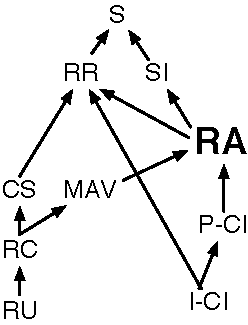
\includegraphics[width=1.3in]{diagram/isolation-graffle.pdf}
\end{center}
\caption{Comparison of RA with isolation levels
  from~\cite{adya,hat-vldb}. RU: Read Uncommitted, RC: Read
  Committed, CS: Cursor Stability, MAV: Monotonic Atomic View, ICI:
  Item Cut Isolation, PCI: Predicate Cut Isolation, RA: Read Atomic,
  SI: Snapshot Isolation, RR: Repeatable Read (Adya \textit{PL-2.99}), S:
  Serializable.}
\label{fig:isolation}
\end{figure}

\subsection{RA and Serializability}
\label{sec:ra-serializable}

When we began this work, we started by examining the use cases
outlined in Section~\ref{sec:motivation} and deriving a weak isolation
guarantee that would be sufficient to ensure their correct
execution. For general-purpose read-write transactions, RA isolation
may indeed lead to non-serializable (and possibly incorrect) database
states and transaction outcomes. Yet, as Section~\ref{sec:usage}
hints, there appears to be a broader ``natural'' pattern for which RA
isolation appears to provide an intuitive (even ``correct'')
semantics. In this section, we show that for transactions
with a particular property of their item read and item write sets, RA is, in
fact, serializable. We define this property, called the
\textit{read-subset-items-written (RSIW) property}, prove that transactions
obeying the RSIW property lead to serializable outcomes, and discuss
the implications of the RSIW property for the applications outlined in
Section~\ref{sec:motivation}.

Because our system model operates on multiple versions, we must make a
small refinement to our use of the term ``serializability''---namely,
we draw a distinction between serial and one-copy serializable
schedules, per Bernstein et al.~\cite{bernstein-book}. First, we say that two histories
$H_1$ and $H_2$ are \textit{view equivalent} if they contain the same
set of committed transactions and have the same operations and $DSG(H_1)$
and $DSG(H_2)$ have the same direct read dependencies. For
consistency with prior work, we say that $T_i$ \textit{reads from}
$T_j$ if $T_i$ directly read-depends on $T_j$. We say that a
transaction is \textit{read-only} if it does not contain write
operations and that a transaction is \textit{write-only} if it does
not contain read operations. In this section, we concern ourselves
with \textit{one-copy serializability}~\cite{bernstein-book}, which we
define using the previous definition of view equivalence.

\begin{definition}[One-Copy Serializability]
  A history is one-copy serializable if it is view equivalent to a serial
  execution of the transactions over a single logical copy of the
  database.
\end{definition}

The basic intuition behind the RSIW property is straightforward: under
RA isolation, if application developers use a transaction to bundle a
set of writes that should be observed together, any transactions that
read from the items that were written will, in fact, behave ``properly''---or
one-copy serializably. That is, for read-only and write-only transactions, if
each reading transaction only reads a subset of the items that another
write-only transaction wrote, then RA isolation is equivalent to
one-copy serializable isolation. Before proving that this behavior is
one-copy serializable, we can more precisely characterize this condition as
follows:

\begin{definition}[Read-Subset-Items-Written] A read-only transaction
  $T_r$ exhibits the \textit{Read-Subset-Items-Written} property if,
  whenever $T_r$ reads a version produced by a write-only transaction
  $T_w$, $T_r$ only reads items written to by $T_w$.
\end{definition}

For example, consider the following History~\ref{hist:rsw}:
\begin{eqnarray}
\label{hist:rsw}
T_1 & w(x_1); w(y_1)\\
T_2 & r(x_1); w(y_1)\nonumber\\
T_3 & r(x_1); r(z_\bot)\nonumber
\end{eqnarray}

Under History~\ref{hist:rsw}, $T_2$ exhibits the RSIW property because
it reads a version produced by transaction $T_1$ and its item read set
($\{x,y\}$) is a subset of $T_1$'s item write set ($\{x,y\}$). However,
$T_3$ does not exhibit the RSIW property because $i.)$ $T_3$ reads from
$T_1$ but $T_3$'s read set ($\{x,z\}$) is not a subset of $T_1$'s
write set ($\{x,y\}$) and $ii.)$, perhaps more subtly, $T_3$ reads
from both $T_1$ and $T_\bot$.

We say that a history $H$ containing read-only and write-only
transactions exhibits the RSIW property (or \textit{has RSIW}) if every read-only transaction
in $H$ exhibits the RSIW property.

This brings us to our main result in this section:

\begin{theorem}
\label{thm:rsw}
If a history $H$ containing read-only and write-only transactions
has RSIW and is valid under RA isolation, then
$H$ is one-copy serializable.
\end{theorem}

The proof of Theorem~\ref{thm:rsw} is by construction: given a history
$H$ has RSIW and is valid under RA isolation, we
describe how to derive an equivalent one-copy serial execution of the
transactions in $H$. We begin with the construction procedure, provide examples
of how to apply the procedure, then prove that the procedure
converts RSIW histories to their one-copy serial equivalents. We
provide the proof in Section~\ref{sec:rsiwproof}

\minihead{Utility} Theorem~\ref{thm:rsw} is helpful because it
provides a simple syntactic condition for understanding when RA will
provide one-copy serializable access. For example, we can apply this
theorem to our use cases from Section~\ref{sec:motivation}. In the
case of multi-entity update and read, if clients issue read-only and
write-only transactions that obey the RSIW property, their result sets
will be one-copy serializable. The RSIW property holds for
equality-based lookup of single records from an index (e.g., fetch
from the index and subsequently fetch the corresponding base tuple,
each of which was written in the same transaction (e.g., was
auto-generated upon insertion of the tuple into the base
relation). However, the RSIW property does not in the event of
multi-tuple reads, leading to less intuitive behavior. Specifically,
if two different clients trigger two separate updates to an index
entry, some clients may observe one update but not the other, and
other clients may observe the opposite behavior. In this case, the
RAMP protocols still provide a snapshot view of the database according
to the index(es)---that is, clients will never observe base data that
is inconsistent with the index entries---but nevertheless surface
non-serializable database states. Finally, for more general
materialized view accesses, point queries and bulk insertions have
RSIW.

As discussed in Section~\ref{sec:motivation}, in the case of indexes
and views, it is helpful to view each physical data structure (e.g.,
a CRDT~\cite{crdt} used to represent an index entry) as a
\textit{collection} of versions. In this case, the RSIW property
applies only if clients make modifications to the entire collection at
once (e.g., as in a \texttt{DELETE CASCADE} operation).

Coupled with an appropriate algorithm ensuring RA isolation, we can
ensure one-copy serializable isolation. This addresses a long-standing
concern with our work: why is RA somehow ``natural'' for these use
cases (but not necessarily all use cases)?  We have encountered
applications that do not require one-copy serializable access---such
as the mailbox unread message maintenance from
Section~\ref{sec:motivation} and, in some cases, index maintenance for
non-read-modify-write workloads---and therefore may safely violate
RSIW. However, we believe the RSIW property is a handy principle (or,
at the least, rule of thumb) for reasoning about applications of RA
isolation and the RAMP protocols.

Finally, the RSIW property is only a \textit{sufficient} condition for
one-copy serializable behavior under RA isolation. It is not
necessary---for example, there are several alternative sufficient
conditions to consider. As a natural extension, while RSIW only
pertains to pairs of read-only and write-only transactions, one might
consider allowing readers to observe multiple write transactions. For
example, consider the following history:
\begin{eqnarray}
\label{hist:rsw-multi-right}
T_1 & w(x_1); w(y_1)\\
T_2 & w(u_2); w(z_2)\nonumber\\
T_3 & r(x_1); r(z_2)\nonumber
\end{eqnarray}
History~\ref{hist:rsw-multi-right} is valid under RA and is also
one-copy serializable but does not have RSIW: $T_3$ reads from
\textit{two} transactions' write sets. However, consider the following
history:
\begin{eqnarray}
\label{hist:rsw-multi-wrong}
T_1: & w(x_1); w(y_1)\\
T_2: & w(u_2); w(z_2)\nonumber\\
T_3: & r(x_1); r(z_\bot)\nonumber\\
T_4: & r(x_\bot); r(z_2)\nonumber
\end{eqnarray}
History~\ref{hist:rsw-multi-wrong} is valid under RA, consists only of
read-only and write-only transactions, yet is no longer
one-copy serializable. $T_3$ observes, in effect, a one-copy serializable prefix
beginning with $T_\bot; T_1$ while $T_4$ observes a prefix beginning
with $T_\bot; T_2$. Neither $T_3$ nor $T_4$ observes the prefixes
$T_\bot; T_1; T_2$ or $T_\bot; T_2; T_1$.

Thus, while there may indeed be useful criteria beyond the RSIW
property that we might consider as a basis for one-copy serializable
execution under RA, we have observed RSIW to be the most intuitive and
useful thus far. One clear criteria is to search for schedules or
restrictions under RA with an acyclic Directed Serialization Graph (from
Appendix~\ref{sec:rsiwproof}). The reason why RSIW is so simple for
read-only and write-only transactions is that each read-only
transaction only reads from one other transaction and does not induce
any additional anti-dependencies. Combining reads and writes
complicates reasoning about the acyclicity of the graph.

This exercise touches upon an important
lesson in the design and use of weakly isolated systems: by
restricting the set of operations accessible to a user (e.g., RSIW
read-only and write-only transactions), one can often achieve more
scalable implementations (e.g., using weaker semantics)
\textit{without} necessarily violating existing abstractions (e.g.,
one-copy serializable isolation). While prior work often focuses on
restricting only operations (e.g., to read-only or write-only
transactions~\cite{eiger,divy-writeonly}, or stored
procedures~\cite{calvin,hstore,jones-dtxn}, or single-site
transactions~\cite{megastore}) or only semantics (e.g., weak isolation
guarantees~\cite{hat-vldb,eiger,explicit-socc}), we see
considerable promise in better understanding the intersection between
and combinations of the two. This is often subtle and almost always
challenging, but the results---as we found here---may be surprising.

 \subsection{System Model and Scalability}
\label{sec:sysmodel}

We consider databases that are partitioned, with the set of items in
the database spread over multiple servers. Each item has a single
logical copy, stored on a server---called the item's
\textit{partition}---whose identity can be calculated using the
item. Clients forward operations on each item to the item's partition,
where they are executed. In our examples, all data items have the null
value ($\bot$) at database initialization. In this section, we do not
model replication of data items within a partition; this can happen at
a lower level of the system than our discussion (see
Section~\ref{sec:replication}) as long as operations on each item are
linearizable~\cite{dcomp-book}.

\minihead{Scalability criteria} As we discussed in
Section~\ref{sec:ramp-motivation}, large-scale deployments often eschew
transactional functionality on the premise that it would be too
expensive or unstable in the presence of failure and degraded
operating
modes~\cite{ladis,tao,bigtable,pnuts,dynamo,helland-trans,2pc-scalability,espresso,rainbird}. Our
goal in this paper is to provide robust and scalable transactional
functionality, and, so we first define criteria for ``scalability'':

\vspace{.5em}\noindent Per Section~\ref{sec:model},
\textit{Coordination-free execution} ensures that one client's
transactions cannot cause another client's to block and that, if a
client can contact the partition responsible for each item in its
transaction, the transaction will eventually commit (or abort of its
own volition). This prevents one transaction from causing another to
abort---which is particularly important in the presence of partial
failures---and guarantees that each client is able to make useful
progress. Note that ``strong'' isolation models like serializability
and Snapshot Isolation require coordination and thus limit
scalability. Locking is an example of a non-coordination-free
implementation mechanism.\vspace{.5em}

Many applications can limit their data accesses to a single
partition via explicit data
modeling~\cite{gstore,espresso,megastore,helland-trans} or
planning~\cite{schism,pavlo-partition}. However, this is not always
possible. In the case of secondary indexing, there is a cost
associated with requiring single-partition updates (scatter-gather
reads), while, in social networks like Facebook and large-scale
hierarchical access patterns as in Rainbird~\cite{rainbird}, perfect partitioning of
data accesses is near-impossible. Accordingly:

\vspace{.5em}\noindent\textit{Partition independence} ensures that, in
order to execute a transaction, a client only contacts partitions for
data items that its transaction directly accesses. Thus, a partition
failure only affects transactions that access items contained on the
partition. This also reduces load on servers not directly involved in
a transaction's execution. In the literature, partition independence
for replicated data is also called \textit{replica
  availability}~\cite{hat-vldb} or \textit{genuine partial
  replication}~\cite{gpr}. Using a centralized validator or scheduler
for transactions is an example of a non-partition-independent
implementation mechanism.\vspace{.5em}

In addition to the above requirements, we limit the \textit{metadata
  overhead} of algorithms. There are many potential solutions for
providing atomic visibility that rely on storing prohibitive amounts
of state. We will attempt to minimize the \textit{metadata}---that is,
data that the transaction did not itself write but which is required
for correct execution. In our algorithms, we will specifically provide
constant-factor metadata overheads (\raps, \rapb) or else overhead
linear in transaction size (but independent of data size; \rapl). As
an example of a solution using prohibitive amounts of metadata, each
transaction could send copies of all of its writes to every partition
it accesses so that readers observe all of its writes by reading a
single item. This provides RA isolation but requires considerable
storage. Other solutions may require extra data storage proportional
to the number of servers in the cluster or, worse, the database size,
which we discuss in Related Work (Chapter~\ref{c.relatedwork}).




\section{RAMP Transaction Algorithms}
\label{sec:ramp-algorithm}

Given specifications for RA isolation and scalability, we present
algorithms for achieving both. For ease of understanding, we first
focus on providing read-only and write-only transactions with a ``last
writer wins'' overwrite policy, then subsequently discuss how to
perform read/write transactions. Our focus in this section is on
intuition and understanding; we defer all correctness and scalability
proofs to Section~\ref{sec:rampproofs}, providing salient details inline.

At a high level, RAMP transactions allow reads and writes to proceed
concurrently. This provides excellent performance but, in turn,
introduces certain race conditions that could cause undesirable
anomalies: one transaction might only read a subset of another
transaction's writes, violating RA (i.e., fractured reads might
occur). Instead of preventing this race (hampering scalability), RAMP
readers \textit{autonomously} detect the race (using metadata attached
to each data item) and fetch any missing, in-flight writes from their
respective partitions. To make sure that readers never have to wait
for writes to arrive at a partition, writers use a two-phase (atomic
commitment) protocol that ensures that once a write is visible to
readers on one partition, any other writes in the transaction are
present on and, if appropriately identified by version, readable from
their respective partitions.

In this section, we present three algorithms that provide a trade-off
between the amount of metadata required and the expected number of
extra reads to fetch missing writes. As discussed in
Section~\ref{sec:motivation}, while techniques like distributed
locking couple mutual exclusion with atomic visibility of writes, RAMP
transactions correctly control visibility but allow concurrent and
scalable execution.

\subsection{RAMP-Fast}
\label{sec:rapl}


\begin{figure}[t!]
\begin{center}
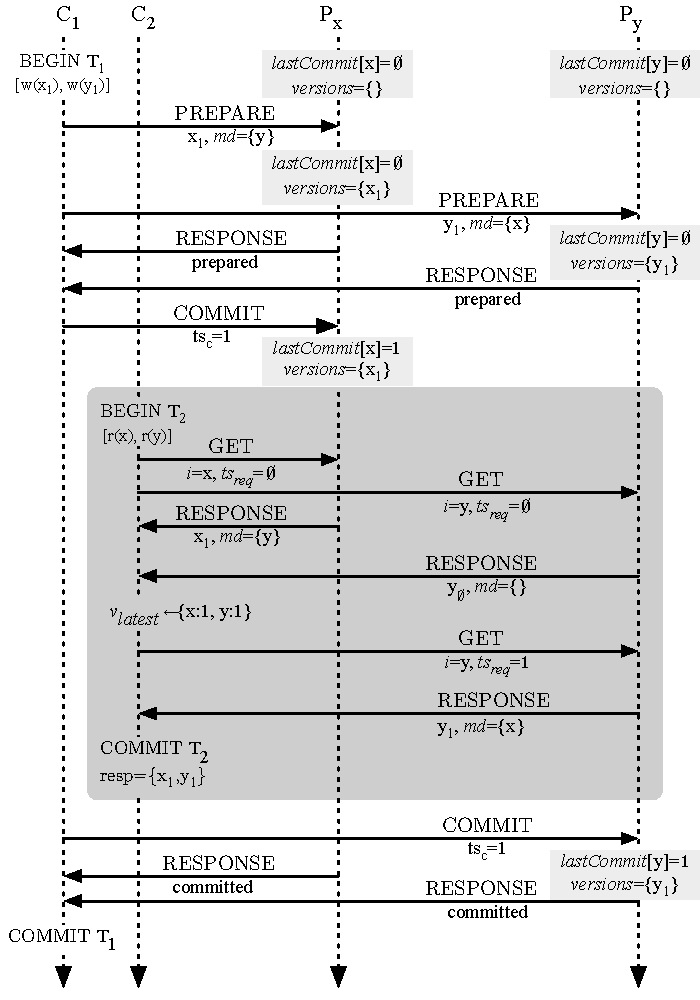
\includegraphics[width=.6\columnwidth]{diagram/rapl-big.pdf}\vspace{.5em}
\caption{Space-time diagram for \rapl execution for two transactions
  $T_1$ and $T_2$ performed by clients $C_1$ and $C_2$ on partitions
  $P_x$ and $P_y$. Lightly-shaded boxes represent current partition
  state ($lastCommit$ and $versions$), while the single darker box
  encapsulates all messages exchanged during $C_2$'s execution of
  transaction $T_2$.  Because $T_1$ overlaps with $T_2$, $T_2$ must
  perform a second round of reads to repair the fractured read between
  $x$ and $y$. $T_1$'s writes are assigned timestamp $1$. In our
  depiction, each item does not appear in its list of writes (e.g.,
  $P_x$ sees $\{y\}$ only and not $\{x,y\}$.}
\label{fig:rapl-execution}
\end{center}
\end{figure}

To begin, we present a RAMP algorithm that, in the race-free case,
requires one RTT for reads and two RTTs for writes, called
\texttt{RAMP-Fast} (abbreviated \rapl; Algorithm~\ref{alg:rapl}).
\rapl stores metadata in the form of write sets (overhead linear in
transaction size).

\minihead{Overview} Each write in \rapl
(lines~\ref{rapl-putall-start}--\ref{rapl-putall-end}) contains a
timestamp (line~\ref{rapl-newid}) that uniquely identifies the writing
transaction as well as a set of items written in the transaction
(line~\ref{rapl-metadata}). For now, combining a unique client ID and
client-local sequence number is sufficient for timestamp generation
(see also Section~\ref{sec:additional}).

\rapl write transactions proceed in two phases: a first round of
communication places each timestamped write on its respective
partition. In this \textsc{prepare} phase, each partition adds the
write to its local database ($versions$,
lines~\ref{rapl-versions},~\ref{rapl-beginprepare-client}--\ref{rapl-endprepare-client}). A
second round of communication
(lines~\ref{rapl-begincommit-client}--\ref{rapl-endcommit-client}) marks versions as committed. In this
\textsc{commit} phase, each partition updates an index containing the
highest-timestamped committed version of each item ($lastCommit$,
lines~\ref{rapl-lc},~\ref{rapl-begincommit-server}--\ref{rapl-endcommit-server}).

\rapl read transactions begin by first fetching the last
(highest-timestamped) committed version for each item from its
respective partition
(lines~\ref{rapl-client-firstround-start}--\ref{rapl-client-secondround-start}). Using
the results from this first round of reads, each reader can calculate
whether it is ``missing'' any versions (that is, versions that were
prepared but not yet committed on their partitions). The reader
calculates a mapping from each item $i$ to the highest timestamped
version of $i$ that appears in the metadata of any version (of $i$ or
of any other item) in the first-round read set
(lines~\ref{rapl-client-latest-start}--\ref{rapl-client-latest-end}). If
the reader has read a version of an item that has a lower timestamp
than indicated in the mapping for that item, the reader issues a
second read to fetch the missing version (by timestamp) from its
partition
(lines~\ref{rapl-client-secondround-start}--\ref{rapl-client-secondround-end}). Once
all missing versions are fetched (which can be done in parallel), the
client can return the resulting set of versions---the first-round
reads, with any missing versions replaced by the optional, second
round of reads.

\minihead{By example} Consider the \rapl execution depicted in
Figure~\ref{fig:rapl-execution}. $T_1$ writes to both $x$ and $y$,
performing the two-round write protocol on two partitions, $P_x$ and
$P_y$. However, $T_2$ reads from $x$ and $y$ while $T_1$ is
concurrently writing.  Specifically, $T_2$ reads from $P_x$
\textit{after} $P_x$ has committed $T_1$'s write to $x$, but $T_2$
reads from $P_y$ \textit{before} $P_y$ has committed $T_1$'s write to
$y$. Therefore, $T_2$'s first-round reads return $x=x_1$ and $y=\bot$,
and returning this set of reads would violate RA. Using the metadata
attached to its first-round reads, $T_2$ determines that it is missing
$y_1$ (since $v_{latest}[y]=1$ and $1 > \bot$) and so $T_2$
subsequently issues a second read from $P_y$ to fetch $y_1$ by
version. After completing its second-round read, $T_2$ can safely
return its result set. $T_1$'s progress is unaffected by $T_2$, and
$T_1$ subsequently completes by committing $y_1$ on $P_y$.



\minihead{Why it works} \rapl writers use metadata as a record of
intent: a reader can detect if it has raced with an in-progress commit
round and use the metadata stored by the writer to fetch the missing
data. Accordingly, \rapl readers only issue a second round of reads in
the event that they read from a partially-committed write transaction
(where some but not all partitions have committed a write). In this
event, readers will fetch the appropriate writes from the
not-yet-committed partitions. Most importantly, \rapl readers never
have to stall waiting for a write that has not yet arrived at a
partition: the two-round \rapl write protocol guarantees that, if a
partition commits a write, all of the corresponding writes in the
transaction are present on their respective partitions (though
possibly not committed locally). As long as a reader can identify the
corresponding version by timestamp, the reader can fetch the version
from the respective partition's set of pending writes without
waiting. To enable this, \rapl writes contain metadata linear in the
size of the writing transaction's write set (plus a timestamp per
write).\vspace{.5em}

\rapl requires two RTTs for writes: one for \textsc{prepare}
and one for \textsc{commit}. For reads, \rapl requires one RTT in the
absence of concurrent writes and two RTTs otherwise.

RAMP timestamps are only used to identify specific versions and in
ordering concurrent writes to the same item; \rapl transactions do not
require a ``global'' timestamp authority. For example, if
$lastCommit[k]=2$, there is no requirement that a transaction
with timestamp $1$ has committed or even that such a transaction
exists.

\begin{algorithm}[t!]
\small
\caption{RAMP-Fast}
\label{alg:rapl}
\newcommand{\myindent}{\hspace{-1em}}

\begin{algorithmic}[1]
\Statex{\textbf{\textit{Server-side Data Structures}}\\
$versions$: set of versions $\langle item, value,$ timestamp $ts_v,$ metadata $md\rangle$ \label{rapl-versions}\\
$lastCommit[i]$: last committed timestamp for item $i$\label{rapl-lc}}\vspace{.5em}

\Statex{\textbf{\textit{Server-side Methods}}}\vspace{.25em}

\Procedure{prepare}{$v$ : version}\label{rapl-beginprepare-server}
  \State $versions$.add($v$)\label{rapl-server-prepare}
  \State \Return
\EndProcedure\vspace{.5em}\label{rapl-endprepare-server}

\Procedure{commit}{$ts_c$ : timestamp}\label{rapl-begincommit-server}
  \State $I_{ts} \gets$ $\{w.item \mid w \in versions \wedge w.ts_v = ts_c\}$\label{rapl-server-commit-1}
  \State $\forall i \in I_{ts}$, $lastCommit[i] \gets
  \max(lastCommit[i], ts_c)$\label{rapl-server-commit-2}
\EndProcedure\vspace{.5em}\label{rapl-endcommit-server}

\Procedure{get}{$i$ : item, $ts_{req}$ : timestamp}\label{rapl-get-server-start}
  \If {$ts_{req} = \emptyset$\label{rapl-get-server-nots-start}}
  \State {\Return $v \in versions : v.item=i \wedge v.ts_v = lastCommit[item]$\label{rapl-get-server-nots-end}}
  \Else 
  \State {\Return $v \in versions : v.item = i \wedge  v.ts_v = ts_{req}$\label{rapl-get-server-withts-end}}
  \EndIf
\EndProcedure\label{rapl-get-server-end}
\Statex\hrulefill\vspace{.25em}

\Statex{\textbf{\textit{Client-side Methods}}}\vspace{.25em}

\Procedure{put\_all}{$W$ : set of $\langle item, value \rangle$}\label{rapl-putall-start}
  \State $ts_{tx} \gets$ generate new timestamp\label{rapl-newid}
  \State $I_{tx} \gets $ set of items in $W$\label{rapl-metadata}
  \ParFor{$\langle i, v\rangle \in W$}\label{rapl-beginprepare-client}
  \State $v \gets \langle item=i, value=v, ts_v=ts_{tx}, md=(I_{tx} - \{i\})\rangle$\label{rapl-prepare-data}
  \State\hspace{1em} invoke $\textsc{prepare}(v)$ on respective server (i.e., partition)\label{rapl-prepare-client}
  \EndParFor\label{rapl-endprepare-client}
  
  \ParFor{server $s : s$ contains an item in $W$}\label{rapl-begincommit-client}
  \State invoke $\textsc{commit}(ts_{tx})$ on $s$\label{rapl-commit-client}
  \EndParFor\label{rapl-endcommit-client}
\EndProcedure\vspace{.5em}\label{rapl-putall-end}

\Procedure{get\_all}{$I$ : set of items}\label{rapl-client-getall-start}
  \State $ret \gets \{\}$\label{rapl-client-firstround-start}
  \ParFor {$i \in I$}
  \State $ret[i] \gets \textsc{get}(i, \emptyset)$\label{rapl-client-firstround-get}
  \EndParFor\vspace{.25em}\label{rapl-client-firstround-end}

  \State $v_{latest} \gets \{\}$ (default value: $-1$)\label{rapl-client-latest-start}
  \For{response $r \in ret$}
  \For{$i_{tx} \in r.md$}
  \State $v_{latest}[i_{tx}] \gets \max(v_{latest}[i_{tx}], r.ts_v)$\label{rapl-client-latest-calculate}
  \EndFor
  \EndFor\vspace{.25em}\label{rapl-client-latest-end}

  \ParFor{item $i \in I$}\label{rapl-client-secondround-start}
  \If{$v_{latest}[i] > ret[i].ts_v$}\label{rapl-client-secondround-check}
  \State $ret[i] \gets \textsc{get}(i, v_{latest}[i])$\label{rapl-client-secondround-get}
  \EndIf
  \EndParFor\vspace{.25em}\label{rapl-client-secondround-end}

  \State \Return $ret$\label{rapl-client-getall-return}
\EndProcedure\label{rapl-client-getall-end}


\end{algorithmic}
\end{algorithm}


\subsection{RAMP-Small: Trading Metadata for RTTs}
\label{sec:raps}

\begin{figure}[t!]
\begin{center}
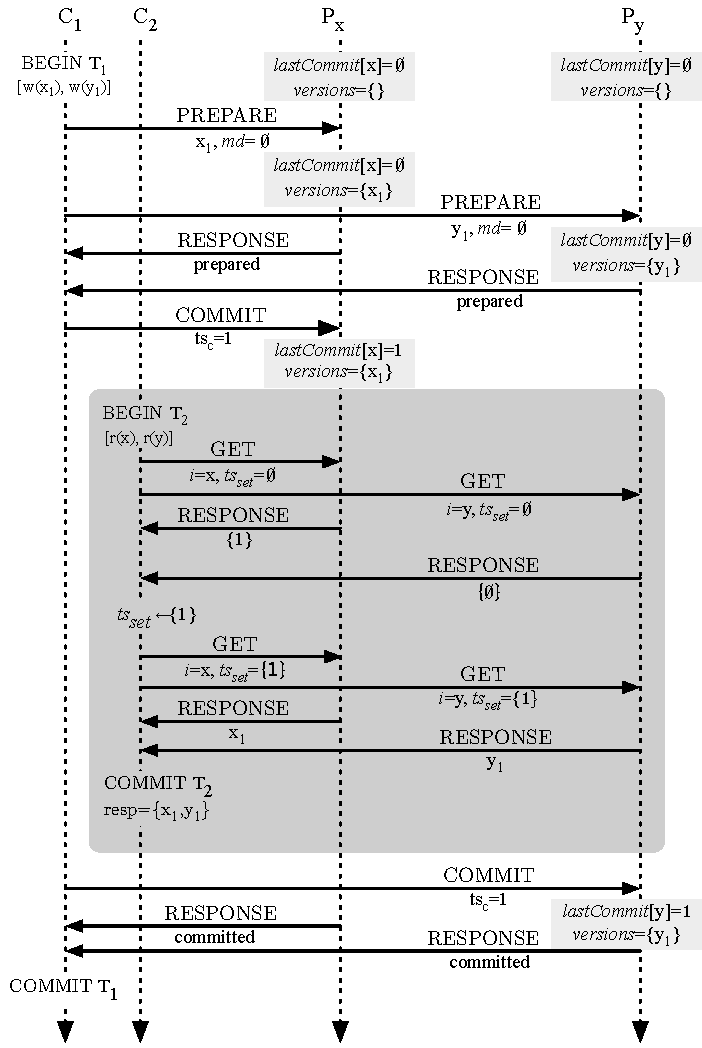
\includegraphics[width=.6\columnwidth]{diagram/raps-big.pdf}\vspace{.5em}
\caption{Space-time diagram for \raps execution for two transactions
  $T_1$ and $T_2$ performed by clients $C_1$ and $C_2$ on partitions
  $P_x$ and $P_y$. Lightly-shaded boxes represent current partition
  state ($lastCommit$ and $versions$), while the single darker box
  encapsulates all messages exchanged during $C_2$'s execution of
  transaction $T_2$. $T_1$ first fetches the highest committed
  timestamp from each partition, then fetches the corresponding
  version. In this depiction, partitions only return timestamps
  instead of actual versions in response to first-round reads.}
\label{fig:raps-execution}
\end{center}
\end{figure}

While \rapl requires metadata size linear in write set size but provides best-case
one RTT for reads, \texttt{RAMP-Small} (\raps) uses constant
metadata but always requires two RTT for reads
(Algorithm~\ref{alg:raps}). \raps and \rapl writes are identical, but,
instead of attaching the entire write set to each write, \raps writers
only store the transaction timestamp
(line~\ref{raps-prepare-data}). Unlike \rapl, \raps readers issue a
first round of reads to fetch the highest committed timestamp for each
item from its respective partition
(lines~\ref{raps-get-server-nots-end},~\ref{raps-client-firstround-start}--\ref{raps-client-firstround-end}). Then
the readers send the entire set of timestamps they received to
the partitions in a second round of communication
(lines~\ref{raps-client-secondround-start}--\ref{raps-client-secondround-end}). For
each item in the read request, \raps servers return the
highest-timestamped version of the item that also appears in the
supplied set of timestamps
(lines~\ref{raps-get-server-withts-start}--\ref{raps-get-server-withts-end}). Readers
subsequently return the results from the mandatory second round of
requests.

\minihead{By example} In Figure~\ref{fig:raps-execution}, under \raps,
$P_x$ and $P_y$ respectively return the sets $\{1\}$ and
$\{\bot\}$ in response to $T_2$'s first round of reads. $T_2$ would
subsequently send the set $\{1, \bot\}$ to both $P_x$ and $P_y$, which
would return $x_1$ and $y_1$.  (Including $\bot$ in the second-round
request is unnecessary, but we leave it in for ease of understanding.)

\minihead{Why it works} In \raps, if a transaction has committed on
some but not all partitions, the transaction timestamp will be
returned in the first round of any concurrent read transaction
accessing the committed partitions' items. In the (required) second
round of read requests, any prepared-but-not-committed partitions will
find the committed timestamp in the reader-provided set and return the
appropriate version. In contrast with \rapl, where readers explicitly
provide partitions with a specific version to return in the (optional)
second round, \raps readers defer the decision of which version to
return to the partition, which uses the reader-provided set to
decide. This saves metadata but increases RTTs, and the size of the
parameters of each second-round \textsc{get} request is (worst-case)
linear in the read set size. Unlike \rapl, there is no requirement to
return the value of the last committed version in the first round
(returning the version, $lastCommit[k]$, suffices in
line~\ref{raps-get-server-nots-end}).

\begin{algorithm}[t!]
\small
\caption{RAMP-Small}
\label{alg:raps}
\newcommand{\myindent}{\hspace{-1em}}
\begin{algorithmic}[1]
\Statex{\textbf{\textit{Server-side Data Structures}}}
\Statex same as in \rapl (Algorithm~\ref{alg:rapl}) \vspace{.5em}

\Statex{\textbf{\textit{Server-side Methods}}}\
\Statex \textsc{prepare}, \textsc{commit} same as in \rapl\vspace{.5em}

\Procedure{get}{$i$ : item, $ts_{set}$ : set of timestamps}\label{raps-get-server-start}
  \If{$ts_{set} = \emptyset$}
  \State \Return $v \in versions : v.item=i \wedge v.ts_v =
  lastCommit[k]$\label{raps-get-server-nots-end}
  \Else
  \State $ts_{match} = \{t \mid t \in ts_{set} \wedge \exists v \in versions : v.item = i \wedge v.t_v = t\}$\label{raps-get-server-withts-start}
  \State \Return $v \in versions : v.item = i \wedge  v.ts_v =
  max(ts_{match})$\label{raps-get-server-withts-end}
  \EndIf

\EndProcedure\label{raps-get-server-end}
\Statex\hrulefill\vspace{.25em}

\Statex{\textbf{\textit{Client-side Methods}}}\vspace{.25em}

\Procedure{put\_all}{$W$ : set of $\langle item, value \rangle$}
\Statex \hspace{1.5em} same as \rapl \textsc{put\_all} but do not instantiate $md$ on line~\ref{rapl-prepare-data}\label{raps-prepare-data}
\EndProcedure\vspace{.5em}\label{raps-putall-end}

\Procedure{get\_all}{$I$ : set of items}\label{raps-client-getall-start}
\State \hspace{.35em} $ts_{set} \gets \{\}$\label{raps-client-firstround-start}
\ParFor {$i \in I$}
    \State $ts_{set}.$add($\textsc{get}(i, \emptyset).ts_v$)\label{raps-client-firstround-get}
  \EndParFor\vspace{.25em}\label{raps-client-firstround-end}

  \State $ret \gets \{\}$
  \ParFor{item $i \in I$}\label{raps-client-secondround-start}
    \State $ret[i] \gets \textsc{get}(i, ts_{set})$ \label{raps-client-secondround-get}
  \EndParFor\vspace{.25em}\label{raps-client-secondround-end}

  \State \Return $ret$\label{raps-client-getall-return}
\EndProcedure\label{raps-client-getall-end}


\end{algorithmic}
\end{algorithm}

\subsection{RAMP-Hybrid: An Intermediate Solution}
\label{sec:rapb}

\texttt{RAMP-Hybrid} (\rapb; Algorithm~\ref{alg:rapb}) strikes a
compromise between \rapl and \raps. \rapb and \raps write protocols
are identical, but, instead of storing the entire write set (as in
\rapl), \rapb writers store a Bloom filter~\cite{bloomfilter}
representing the transaction write set
(line~\ref{rapb-putall-start}). \rapb readers proceed as in \rapl, with
a first round of communication to fetch the last-committed version of
each item from its partition
(lines~\ref{rapb-client-firstround-start}--\ref{rapb-client-firstround-end}). Given
this set of versions, \rapb readers subsequently compute a list of
\textit{potentially} higher-timestamped writes for each item
(lines~\ref{rapb-client-compute-start}--\ref{rapb-client-compute-end}). Any
potentially missing versions are fetched in a second round of reads
(lines~\ref{rapb-client-secondround-start}).

\minihead{By example} In Figure~\ref{fig:rapl-execution}, under \rapb,
$x_1$ would
contain a Bloom filter with positives for $x$ and $y$ and $y_{\bot}$
would contain an empty Bloom filter. $T_2$ would check for the
presence of $y$ in $x_1$'s Bloom filter (since $x_1$'s version is $1$
and $1 > \bot$) and, finding a match, conclude that it is potentially
missing a write ($y_1$). $T_2$ would subsequently fetch $y_1$ from
$P_y$.

\minihead{Why it works} \rapb is effectively a hybrid between \rapl
and \raps. If the Bloom filter has no false positives, \rapb reads
behave like \rapl reads. If the Bloom filter has all false positives,
\rapb reads behave like \raps reads. Accordingly, the number of
(unnecessary) second-round reads (i.e., which would not be performed
by \rapl) is controlled by the Bloom filter false positive rate, which
is in turn (in expectation) proportional to the size of the Bloom
filter. Any second-round \textsc{get} requests are accompanied by a
set of timestamps that is also proportional in size to the false
positive rate.  Therefore, \rapb exposes a trade-off between metadata
size and expected performance. To understand why \rapb is safe, we
simply have to show that any false positives (second-round reads) will
not compromise the integrity of the result set; with unique
timestamps, any reads due to false positives will return null.

\begin{algorithm}[t!]
\small
\caption{RAMP-Hybrid}
\label{alg:rapb}
\newcommand{\myindent}{\hspace{-1em}}
\begin{algorithmic}[1]
\Statex{\textbf{\textit{Server-side Data Structures}}}
\Statex same as in \rapl (Algorithm~\ref{alg:rapl}) \vspace{.5em}

\Statex{\textbf{\textit{Server-side Methods}}}\
\Statex \textsc{prepare}, \textsc{commit} same as in \rapl
\Statex \textsc{get} same as in \raps
\Statex\hrulefill\vspace{.25em}

\Statex{\textbf{\textit{Client-side Methods}}}\vspace{.25em}

\Procedure{put\_all}{$W$ : set of $\langle item, value \rangle$}~\label{rapb-putall-start}
\Statex \hspace{1.5em} same as \rapl \textsc{put\_all} but instantiate $md$ on line~\ref{rapl-prepare-data}
\Statex \hspace{1.5em} with Bloom filter containing $I_{tx}$
\EndProcedure\vspace{.5em}\label{rapb-putall-end}

\Procedure{get\_all}{$I$ : set of items}\label{rapb-client-getall-start}
  \State $ret \gets \{\}$\label{rapb-client-firstround-start}
  \ParFor {$i \in I$}
  \State $ret[i] \gets \textsc{get}(i, \emptyset)$\label{rapb-client-firstround-get}
  \EndParFor\vspace{.25em}\label{rapb-client-firstround-end}

  \State $v_{fetch} \gets \{\}$

  \For{version $v \in ret$}\label{rapb-client-compute-start}
  \For{version $v' \in ret: v' \neq v$}
  \If{$v.ts_v > v'.ts_v \wedge v.md.lookup(v'.item) \rightarrow True$}
    \State $v_{fetch}[v'.item]$.add($v.ts_v$)\label{rapb-client-compute-step}
  \EndIf
  \EndFor
  \EndFor\label{rapb-client-compute-end}

  \ParFor{item $i \in v_{fetch}$}\label{rapb-client-secondround-start}
        \State $ret[i] \gets \textsc{get}(k, v_{fetch}[i])$ \textbf{if}
        $\textsc{get}(k, v_{fetch}[i]) \neq \bot$ \label{rapb-client-secondround-get}
  \EndParFor\vspace{.25em}\label{rapb-client-secondround-start}
  \State \Return $ret$\label{rapb-client-getall-return}
\EndProcedure\label{rapb-client-getall-end}


\end{algorithmic}
\end{algorithm}


\subsection{Summary and Additional Details}

The RAMP algorithms allow readers to safely race writers without
requiring either to stall. The metadata attached to each write allows
readers in all three algorithms to safely handle concurrent and/or
partial writes and in turn allows a trade-off between metadata size
and performance (Table~\ref{table:rap-compare}): \rapl is optimized
for fast reads, \raps is optimized for small metadata, and \rapb is,
as the name suggests, a middle ground. \rapl requires metadata linear
in transaction size, while \raps and \rapb require constant
metadata. However, \raps and \rapb require more RTTs for reads
compared to \rapl when there is no race between readers and
writers. When reads and writes race, in the worst case, all algorithms
require two RTTs for reads.  Writes always require two RTTs to prevent
readers from stalling due to missing, unprepared writes.

RAMP algorithms are scalable because clients only contact partitions
directly accessed by their transactions (partition independence), and clients
cannot stall one another (are coordination-free). More
specifically, readers do not interfere with other readers, writers do
not interfere with other writers, and readers and writers can proceed
concurrently. When a reader races a writer to the same items, the
writer's new versions will only become visible to the reader (i.e., be
committed) once it is guaranteed that the reader will be able to fetch
all of them (possibly via a second round of communication). A reader
will \textit{never} have to stall waiting for writes to arrive at a
partition (for details, see Invariant~\ref{inv:suitable-present} in
the Appendix); however, the reader may have to contact the servers
twice in order to fetch any versions that were missing from its first
set of reads.


\begin{table}
\begin{center}
{
\begin{tabular}{|c|c|c|c|c|c|c|}
\hline
\multirow{2}{*}{\textbf{Algorithm}} & \multicolumn{3}{c|}{\textbf{RTTs/transaction}} & \multicolumn{2}{c|}{\textbf{Metadata (+stamp)}} \\
 & \multicolumn{1}{c}{W} & \multicolumn{1}{c}{R (stable)} & \multicolumn{1}{c|}{R ($O$)}& \multicolumn{1}{c}{\small Stored} & \multicolumn{1}{c|}{\small Per-Request}\\\hline

{ \rapl} & { 2 } & {1} & {2} & { txn items } & - \\
{ \raps} & { 2 } &  {2} & {2} & - & { stamp/item} \\
{ \rapb} & { 2 } & {$1+\epsilon$} & {2} & { Bloom filter} & { stamp/item}\\\hline
\end{tabular}}
\caption{Comparison of basic algorithms: RTTs required for writes (W),
  reads (R) without concurrent writes and in the worst case ($O$),
  stored metadata and metadata attached to read requests (in addition 
  to a timestamp for each). \label{table:rap-compare}}
\end{center}



\end{table}

\label{sec:additional}

Below, we discuss relevant implementation details.

\minihead{Multi-versioning and garbage collection} RAMP transactions
rely on multi-versioning to allow readers to access versions that have
not yet committed and/or have been overwritten. In our pseudocode, we
have presented an implementation based on multi-versioned storage; in
practice, multi-versioning can be implemented by using a
single-versioned storage engine for retaining the last committed
version of each item and using a ``look-aside'' store for access to
both prepared-but-not-yet-committed writes and (temporarily) any
overwritten versions. The look-aside store should make prepared
versions durable but can---at the risk of aborting transactions in the
event of a server failure---simply store any overwritten versions in
memory. Thus, with some work, RAMP algorithms are portable to non-multi-versioned storage systems.

In both architectures, each partition's data will grow without bound
if old versions are not removed. If a committed version of an item is
not the highest-timestamped committed version (i.e., a committed
version $v$ of item $k$ where $v < lastCommit[k]$), it can be safely
discarded (i.e., garbage collected, or GCed) as long as no readers
will attempt to access it in the future (via second-round \textsc{get}
requests). It is easiest to simply limit the running time of read
transactions and GC overwritten versions after a fixed amount of real
time has elapsed. Any read transactions that take longer than this GC
window can be restarted~\cite{cops,eiger}. Therefore, the maximum
number of versions retained for each item is bounded by the item's
update rate, and servers can reject any client \textsc{get} requests
for versions that have been GCed (and the read transaction can be
restarted). This violates availability under asynchronous network
behavior, so, as a fallback and a more principled solution, partitions
can also gossip the timestamps of items that have been overwritten and
have not been returned in the first round of any ongoing read
transactions. Under \rapl, if a second-round read request arrives a
server and the server does not have that version due to garbage
collection, it can safely ignore the request or signal failure.

\minihead{Read-write transactions} Until now, we have focused on
read-only and write-only transactions. However, we can extend our
algorithms to provide read-write transactions. If transactions
pre-declare the data items they wish to read, then the client can
execute a \textsc{get\_all} transaction at the start of transaction
execution to pre-fetch all items; subsequent accesses to those items
can be served from this pre-fetched set. Clients can buffer any writes
and, upon transaction commit, send all new versions to servers (in
parallel) via a \textsc{put\_all} request. As in
Section~\ref{sec:ra-def}, this may result in anomalies due to
concurrent update but does not violate RA isolation. Given the
benefits of pre-declared read/write
sets~\cite{schism,pavlo-partition,calvin} and write
buffering~\cite{spanner,f1}, we believe this is a reasonable
strategy. For secondary index lookups, clients can first look up
secondary index entries then subsequently (within the same
transaction) read primary data (specifying versions from index entries as
appropriate).

\minihead{Timestamps} Timestamps should be unique across transactions,
and, for ``session'' consistency (Appendix), increase on a per-client
basis. Given unique client IDs, a client ID and sequence number form
unique transaction timestamps without coordination. Without unique
client IDs, servers can assign unique timestamps with high probability
using UUIDs and by hashing transaction contents.

\minihead{Overwrites} In our algorithms, versions are overwritten
according to a highest-timestamp-wins policy. In practice, and, for
commutative updates, users may wish to employ a different policy upon
\textsc{commit}: for example, perform set union. In this case,
$lastCommit[k]$ contains an abstract data type (e.g., set of versions)
that can be updated with a $merge$
operation~\cite{dynamo,sessionguarantees} (instead of
$updateIfGreater$) upon commit. This treats each committed record as a
set of versions, requiring additional metadata (that can be GCed as in
Section~\ref{sec:optimizations}).


\subsection{Distribution and Fault Tolerance}
\label{sec:replication}

RAMP transactions operate in a distributed setting, which poses
challenges due to latency, partial failure, and network
partitions. Under coordination-free execution, failed clients do not
cause other clients to fail, while partition independence ensures that
clients only have to contact partitions for items in their
transactions. This provides fault tolerance and availability as long
as clients can access relevant partitions. In this section, we address
incident concerns. First, replication can be used to increase the
number of servers hosting a partition, thus increasing
availability. Second, we describe the RAMP protocol behavior when
clients are unable to contact servers.

\minihead{Replication} RAMP protocols can benefit from a variety of
mechanisms including traditional database master-slave replication
with failover, quorum-based protocols, and state machine replication,
which increase the number of physical servers that host a given data
item~\cite{bernstein-book}. To improve durability, RAMP clients can
wait until the effects of their operations (e.g., modifications to
\textit{versions} and \textit{lastCommit}) are persisted to multiple
physical servers before returning from \textsc{put\_all} calls (either
via master-to-slave replication or via quorum replication and by
performing two-phase commit across multiple active servers). Notably,
because RAMP transactions can safely overlap in time, replicas can
process different transactions' \textsc{prepare} and \textsc{commit}
requests in parallel. Availability can also benefit in many protocols,
such as quorum replication. We discuss more advanced replication
techniques in Section~\ref{sec:multidc}.

\minihead{Stalled Operations} RAMP writes use a two-phase atomic
commitment protocol that ensures readers never block waiting for
writes to arrive. As discussed in Section~\ref{sec:motivation}, every
ACP may block during failures~\cite{bernstein-book}. However, under 
coordination-free execution, a blocked transaction (due to failed
clients, failed servers, or network partitions) cannot cause other
transactions to block. Stalled writes act only as ``resource
leaks'' on partitions: partitions will retain prepared versions
indefinitely unless action is taken.

To ``free'' these leaks, RAMP servers can use the Cooperative
Termination Protocol (CTP) described in~\cite{bernstein-book}. CTP can
always complete the transaction except when every partition has
performed \textsc{prepare} but no partition has performed
\textsc{commit}. In CTP, if a server $S_p$ has performed
\textsc{prepare} for transaction $T$ but times out waiting for a
\textsc{commit}, $S_p$ can check the status of $T$ on any other
partitions for items in $T$'s write set. If another server $S_c$ has
received \textsc{commit} for $T$, then $S_p$ can \textsc{commit}
$T$. If $S_a$, a server responsible for an item in $T$, has not
received \textsc{prepare} for $T$, $S_a$ and $S_p$ can promise never
to \textsc{prepare} or \textsc{commit} $T$ in the future and $S_p$ can
safely discard its versions.  Under CTP, if a client blocks
mid-\textsc{commit}, the servers will ensure that the writes will
eventually \textsc{commit} and therefore become visible on all
partitions. A client recovering from a failure can read from the
servers to determine if they unblocked its write.

CTP only runs when writes
block (or time-outs fire) and runs \textit{asynchronously} with
respect to other operations. CTP requires that \textsc{prepare}
messages contain a list of servers involved in the transaction (a
subset of \rapl metadata but a superset of \rapb and \raps) and that
servers remember when they \textsc{commit} and ``abort'' writes (e.g.,
in a log file). Compared to alternatives (e.g., replicating
clients~\cite{paxos-commit}), we have found CTP to be both lightweight
and effective. We evaluate CTP in Section~\ref{sec:ctp}.

\subsection{Additional Semantics}
\label{sec:ramp-semantics}

While our RAMP transactions provide RA isolation, they also provide a
number of additional useful guarantees. With linearizable servers,
once a user's operation completes, all other users will observe its
effects (regular register semantics, applied at the transaction
level); this provides a notion of real-time recency. This also ensures
that each user's operations are visible in the order in which they are
committed. Our RAMP implementations provide a variant of PRAM
consistency, where, for each item, each user's writes are
serialized~\cite{pram} (i.e., ``session''
ordering~\cite{daudjee-session}). For example, if a user updates her
privacy settings and subsequently posts a new photo, the photo cannot
be read without the privacy setting change~\cite{pnuts}. However, PRAM
does not respect the \textit{happens-before}
relation~\cite{lamportclocks} across users (or missing dependencies, as
discussed in Section~\ref{sec:ra-compare}). If Sam reads Mary's
comment and replies to it, other users may read Sam's comment without
Mary's comment. We further discuss this issue in
Section~\ref{sec:causal}.

\subsection{Further Optimizations}
\label{sec:optimizations}

\noindent RAMP algorithms also allow several possible optimizations:

\minihead{Faster commit detection} If a server returns a version in
response to a \textsc{get} request, then the transaction that created
the version must have issued a \textsc{commit} on at least one
server. In this case, the server can safely mark the version as
committed and update $lastCommit$. This means that the transaction
commit will be reflected in any subsequent \textsc{get} requests that
read from $lastCommit$ for this item---even though the \textsc{commit}
message from the client may yet be delayed. The net effect is that the
later \textsc{get} requests may not have to issue second-round reads
to fetch the versions that otherwise would not have been marked as
committed. This scenario will occur when all partitions have performed
\textsc{prepare} and at least one server but not all partitions have
performed \textsc{commit} (as in CTP). This allows faster updates to
$lastCommit$ (and therefore fewer expected \rapl and \rapb RTTs).

\minihead{Metadata garbage collection} Once all of transaction $T$'s
writes are committed on each respective partition (i.e., are reflected in
$lastCommit$), readers are guaranteed to read $T$'s writes (or later
writes). Therefore, non-timestamp metadata for $T$'s writes stored in
\rapl and \rapb (write sets and Bloom filters) can be
discarded. Detecting that all servers have performed \textsc{commit}
can be performed asynchronously via a third round of communication
performed by either clients or servers.

\minihead{One-phase writes} We have considered two-phase writes, but,
if a user does not wish to read her writes (thereby sacrificing
session guarantees outlined in Section~\ref{sec:ramp-semantics}), the
client can return after issuing its \textsc{prepare} round (without
sacrificing durability). The client can subsequently execute the
\textsc{commit} phase asynchronously, or, similar to optimizations
presented in Paxos Commit~\cite{paxos-commit}, the servers can
exchange \textsc{prepare} acknowledgments with one another and decide
to \textsc{commit} autonomously. This optimization is safe because
multiple \textsc{prepare} phases can safely overlap. We leverage a
similar observation in Section~\ref{sec:multidc}.



\section{Experimental Evaluation}
\label{sec:evaluation}
\label{sec:ramp-evaluation}

We proceed to experimentally demonstrate RAMP transaction scalability
as compared to existing transactional and non-transactional
mechanisms. \rapl, \rapb, and often \raps outperform existing
solutions across a range of workload conditions while exhibiting
overheads typically within $8\%$ and no more than $48\%$ of peak
throughput. As expected from our theoretical analysis, the performance
of our RAMP algorithms does not degrade substantially under contention
and scales linearly to over $7.1$ million operations per second on
$100$ servers. These outcomes validate our goal of coordination-free
design.

\subsection{Experimental Setup}
\label{sec:setup}

To demonstrate the effect of concurrency control on performance and
scalability, we implemented several concurrency control algorithms in
a partitioned, multi-versioned, main-memory database prototype. Our
prototype is in Java and employs a custom RPC system for
serialization. Servers are arranged as a distributed hash
table~\cite{chord} with partition placement determined by random
hashing of keys to servers. As in stores like Dynamo~\cite{dynamo},
clients can connect to any server to execute operations, which the
server will perform on their behalf (i.e., each server acts as a
client in our RAMP pseudocode). We implemented \rapl, \raps, and \rapb
and configure a wall-clock GC window of $5$ seconds as described in
Section~\ref{sec:additional}. \rapb uses a $256$-bit Bloom filter
based on an implementation of MurmurHash2.0~\cite{murmurhash}, with
four hashes per entry; to demonstrate the effects of filter
saturation, we do not modify these parameters in our experiments. Our
prototype utilizes the faster commit detection optimization from
Section~\ref{sec:additional}. We chose not to employ metadata garbage
collection and one-phase writes in order to preserve session
guarantees and because metadata overheads were generally minor.

\minihead{Algorithms for comparison} As a baseline, we do not employ
any concurrency control (denoted \nwnr, for no write and no read
locks); reads and writes take one RTT and are executed in parallel.

We also consider three lock-based mechanisms~\cite{gray-isolation}: long write locks and
long read locks, providing Repeatable Read
isolation (\textit{PL-2.99}; denoted \lwlr), long write locks with short read
locks, providing Read Committed isolation (\textit{PL-2L}; denoted
\lwsr; does not provide RA), and long write locks with no read locks,
providing Read Uncommitted isolation (\lwnr;
also does not provide RA). While only \lwlr provides RA, \lwsr and
\lwnr provide a useful basis for comparison, particularly in measuring
concurrency-related locking overheads. To avoid deadlocks, the system
lexicographically orders lock requests by item and performs them
sequentially. When locks are not used (as for reads in \lwnr and reads
and writes for \nwnr), the system parallelizes operations.

We also consider an algorithm where, for each transaction, designated
``coordinator'' servers enforce RA isolation---effectively, the Eiger
system's 2PC-PCI mechanism~\cite{eiger} (denoted \mstr;
Chapter~\ref{c.relatedwork}). Writes proceed via prepare and commit
rounds, but any reads that arrive at a partition and while a write
transaction to the same item is pending must contact a (randomly chosen,
per-write-transaction) ``coordinator'' partition to determine whether
the coordinator's prepared writes have been committed. Writes require
two RTTs, while reads require one RTT during quiescence and two RTTs
in the presence of concurrent updates (to a variable number of
coordinator partitions---linear in the number of concurrent writes to
the item). Using a coordinator violates partition independence
but---in this case---is still coordination-free. We optimize 2PC-PCI reads by having
clients determine a read timestamp for each transaction (eliminating
an RTT) and do not include happens-before metadata.

This range of lock-based strategies (\lwnr, \lwsr, \lwnr), recent
comparable approach (\mstr), and best-case (\nwnr; no concurrency
control) baseline provides a spectrum of strategies for comparison.

% espresso: 1000:1, f1 via spanner: 

\minihead{Environment and benchmark} We evaluate each algorithm using
the YCSB benchmark~\cite{ycsb} and deploy variably-sized sets of
servers on public cloud infrastructure. We employ \texttt{cr1.8xlarge}
instances on Amazon EC2 and, by default, deploy five partitions on
five servers. We group sets of reads and sets of writes into read-only
and write-only transactions (default size: 4 operations), and use the
default YCSB workload (\texttt{workloada}, with Zipfian distributed
item accesses) but with a 95\% read and 5\% write proportion, reflecting
read-heavy applications
(Section~\ref{sec:motivation},~\cite{tao,eiger,rainbird}; e.g., Tao's
500 to 1 reads-to-writes~\cite{tao,eiger}, Espresso's 1000 to 1
Mailbox application~\cite{espresso}, and Spanner's 3396 to 1
advertising application~\cite{spanner}).

By default, use $5000$ YCSB clients distributed across 5 separate EC2
instances. As in stock YCSB, each client makes a sequence of
synchronous requests to the database. When we later vary the number of
clients, we keep the number of servers hosting the clients fixed. To
fully expose our metadata overheads, use a value size of 1 byte per
write. We found that lock-based algorithms were highly inefficient for
YCSB's default 1000 item database, so we increased the database size
to one million items by default to decrease contention. Each version
contains a timestamp ($64$ bits), and, with YCSB keys (i.e., item IDs)
of size 11 bytes and a transaction length $L$, \rapl requires 11$L$
bytes of metadata per version, while \rapb requires 32 bytes. We
successively vary several parameters, including number of clients,
read proportion, transaction length, value size, database size, and
number of servers and report the average of three sixty-second trials.

\subsection{Experimental Results: Comparison}
\label{sec:eval-compare}

Our first set of experiments focuses on two metrics: performance
compared to baseline and performance compared to existing
techniques. The overhead of RAMP algorithms is typically less than
8\% compared to baseline (\nwnr) throughput, is sometimes zero, and
is never greater than 50\%. \rapl and \rapb always outperform the
lock-based and \mstr techniques, while \raps outperforms lock-based
techniques and often outperforms \mstr. We proceed to demonstrate this
behavior over a variety of conditions:



\minihead{Number of clients} RAMP performance scales well with
increased load and incurs little overhead
(Figure~\ref{fig:clients}). With few concurrent clients, there are few
concurrent updates and therefore few second-round reads; performance
for \rapl and \rapb is close to or even matches that of \nwnr. At peak
throughput with 10,000 clients, \rapl and \rapb pay a throughput
overhead of 4.2\% compared to \nwnr. \rapl and \rapb exhibit
near-identical performance; the \rapb Bloom filter triggers few false
positives and therefore few extra RTTs compared to \rapl. \raps
incurs greater overhead and peaks at almost 60\% of the throughput
of \nwnr. Its guaranteed two-round trip reads are expensive and it
acts as an effective lower bound on \rapl and \rapb performance. In
all configurations, the algorithms achieve low latency. \rapl, \rapb,
\nwnr less than 35~ms on average and less than 10~ms at 5,000
clients; \raps less than 53~ms, 14.3~ms at 5,000 clients.



In comparison, the remaining algorithms perform less favorably. In
contrast with the RAMP algorithms, \mstr servers must check a
coordinator server for each in-flight write transaction to determine
whether to reveal writes to clients. For modest load, the overhead of
these commit checks places \mstr performance between that of \raps and
\rapb.  Under YCSB's Zipfian workload, there is a high probability
that the several ``hot'' keys in the workload have a pending write,
requiring a \mstr commit check. The number of in-flight writes further
increases with load, increasing the number of \mstr commit
checks. This in turn decreases throughput, and, with 10,000 concurrent
clients, \mstr performs so many commit checks per read that it
underperforms the \lwnr lock-based scheme. Under this configuration,
more than 20\% of reads trigger a commit check, and, on servers with
hot items, each commit check requires indirected coordinator checks
for an average of 9.84 transactions. Meanwhile, multi-partition
locking is expensive~\cite{pavlo-partition}: with 10,000 clients, the
most efficient algorithm, \lwnr, attains only 28.6\% of the
throughput of \nwnr, while the least efficient, \lwlr, attains only
1.6\% and peaks at 3,412 transactions per second.


\begin{figure}[th!]
\begin{center}
{
\includegraphics[width=\textwidth]{figs/legend-oneline.pdf}\vspace{0em}}
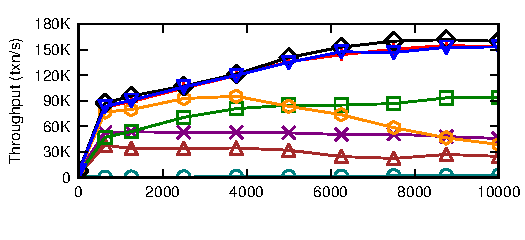
\includegraphics[width=.65\columnwidth]{figs/threads-thru.pdf}\vspace{-2em}
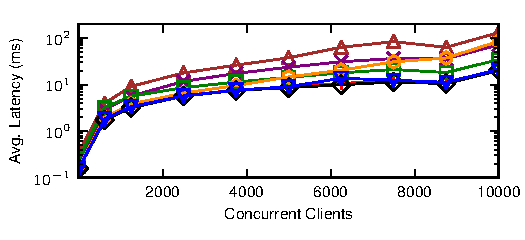
\includegraphics[width=.65\columnwidth]{figs/threads-lat.pdf}
\end{center}\vspace{-.5em}
\caption{Throughput and latency under varying client load. We omit
  latencies for \lwlr, which peaked at over 1.5s.}
\label{fig:clients}
\end{figure}


\begin{figure}[th!]
\begin{center}

\includegraphics[width=\textwidth]{figs/legend-oneline.pdf}\vspace{0em}
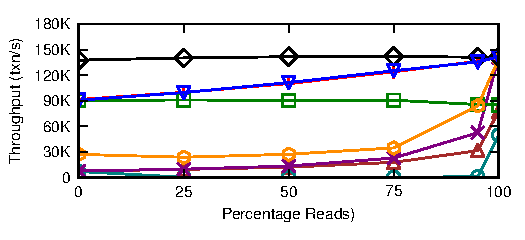
\includegraphics[width=.65\columnwidth]{figs/rprop-thru.pdf}\vspace{-1em}
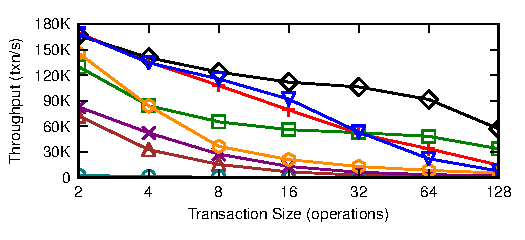
\includegraphics[width=.65\columnwidth]{figs/txnlen-thru.pdf}\vspace{-1em}
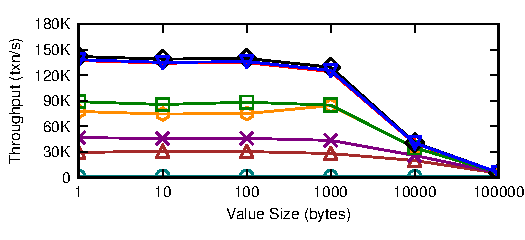
\includegraphics[width=.65\columnwidth]{figs/valuesize-thru.pdf}\vspace{-1em}
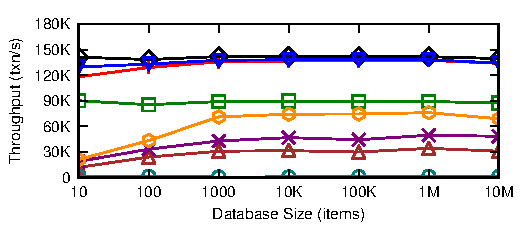
\includegraphics[width=.65\columnwidth]{figs/numkeys-thru.pdf}
\end{center}
\caption{Algorithm performance across varying workload
  conditions. \rapl and \rapb exhibit similar performance to \nwnr
  baseline, while \raps's 2 RTT reads incur a greater performance penalty
  across almost all configurations. RAMP transactions consistently
  outperform RA isolated alternatives.}
\label{fig:others}
\end{figure}

We subsequently varied several other workload parameters, which we
discuss below and plot in Figure~\ref{fig:others}:

\minihead{Read proportion} Increased write activity leads to a greater
number of races between reads and writes and therefore additional
second-round RTTs for \rapl and \rapb reads. With all write
transactions, all RAMP algorithms are equivalent (two RTT) and achieve
approximately 65\% of the throughput of \nwnr. With all reads, \rapl,
\raps, \nwnr, and \mstr are identical, with a single RTT. Between
these extremes, \rapl and \raps scale near-linearly with the write
proportion. In contrast, lock-based protocols fare poorly as
contention increases, while \mstr again incurs penalties due to commit
checks.


\minihead{Transaction length} Increased transaction lengths have
variable impact on the relative performance of RAMP
algorithms. Coordination-free execution ensures long-running
transactions are not penalized, but, with longer transactions,
metadata overheads increase. \rapl relative throughput decreases due
to additional metadata (linear in transaction length) and \rapb
relative performance also decreases as its Bloom filters
saturate. (However, YCSB's Zipfian-distributed access patterns result
in a non-linear relationship between length and throughput.) As
discussed above, we explicitly decided not to tune \rapb Bloom filter
size, but a logarithmic increase in filter size could improve \rapb
performance for large transaction lengths (e.g., 1024 bit filters
should lower the false positive rate for transactions of length 256
from over 92\% to slightly over 2\%).

\minihead{Value size} Value size similarly does not seriously impact
relative throughput. At a value size of 1B, \rapl is within 2.3\% of
\nwnr. However, at a value size of 100KB, \rapl performance nearly
matches that of \nwnr: the overhead due to metadata decreases, and
write request rates slow, decreasing concurrent writes (and
subsequently second-round RTTs). Nonetheless, absolute throughput
drops by a factor of 24 as value sizes moves from 1B to 100KB\@.

\minihead{Database size} RAMP algorithms are robust to high contention
for a small set of items: with only 1000 items in the database, \rapl
achieves throughput within 3.1\% of \nwnr. RAMP algorithms are
largely agnostic to read/write contention, although, with fewer items
in the database, the probability of races between readers and
in-progress writers increases, resulting in additional second-round
reads for \rapl and \rapb. In contrast, lock-based algorithms fare
poorly under high contention, while \mstr indirected commit checks
again incurred additional overhead. By relying on clients (rather than
additional partitions) to repair fractured writes, \rapl, \rapb, and
\raps performance is less affected by hot items. \vspace{.5em}

Overall, \rapl and \rapb exhibit performance close to that of no
concurrency control due to their independence properties and
guaranteed worst-case performance. As the proportion of writes
increases, an increasing proportion of \rapl and \rapb operations take
two RTTs and performance trends towards that of \raps, which provides
a constant two RTT overhead. In contrast, lock-based protocols perform
poorly under contention while \mstr triggers more commit checks than
\rapl and \rapb trigger second round reads (but still performs well
without contention and for particularly read-heavy workloads). The
ability to allow clients to independently verify read sets enables
good performance despite a range of (sometimes adverse) conditions
(e.g., high contention).


\begin{comment}
\begin{figure*}
\begin{center}

\includegraphics[width=.9\textwidth]{figs/legend-oneline.pdf}
\begin{minipage}[b]{0.49\linewidth}
\centering
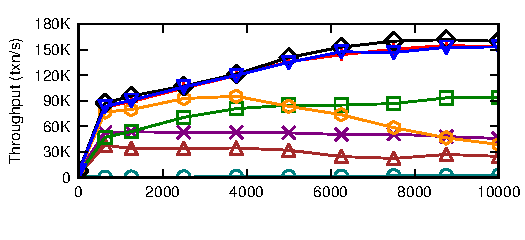
\includegraphics[width=\textwidth]{figs/threads-thru.pdf}
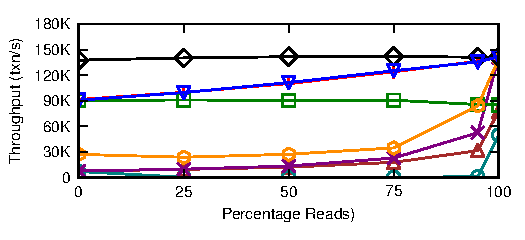
\includegraphics[width=\textwidth]{figs/rprop-thru.pdf}
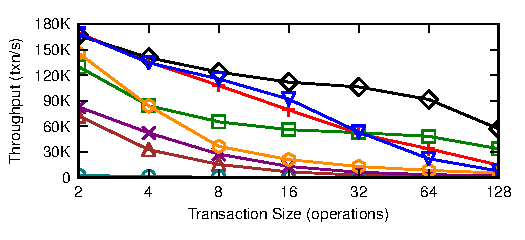
\includegraphics[width=\textwidth]{figs/txnlen-thru.pdf}
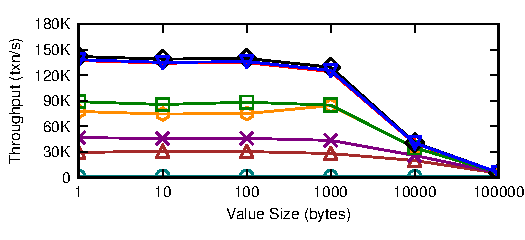
\includegraphics[width=\textwidth]{figs/valuesize-thru.pdf}
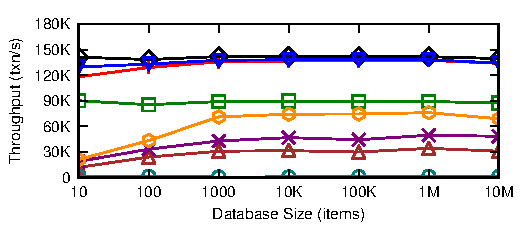
\includegraphics[width=\textwidth]{figs/numkeys-thru.pdf}
\end{minipage}
\begin{minipage}[b]{0.49\linewidth}
\centering
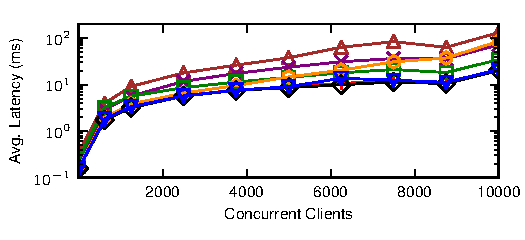
\includegraphics[width=\textwidth]{figs/threads-lat.pdf}
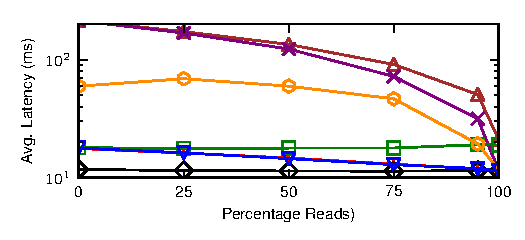
\includegraphics[width=\textwidth]{figs/rprop-lat.pdf}
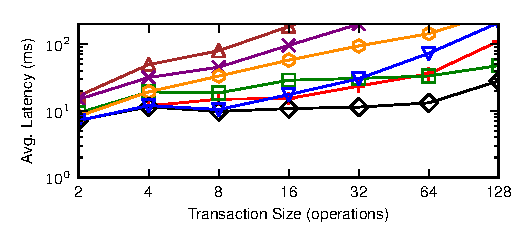
\includegraphics[width=\textwidth]{figs/txnlen-lat.pdf}
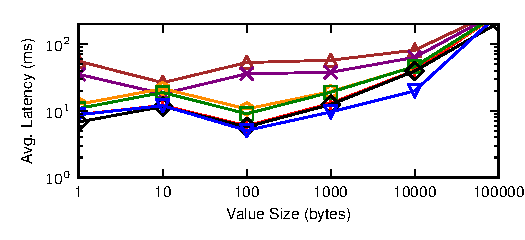
\includegraphics[width=\textwidth]{figs/valuesize-lat.pdf}
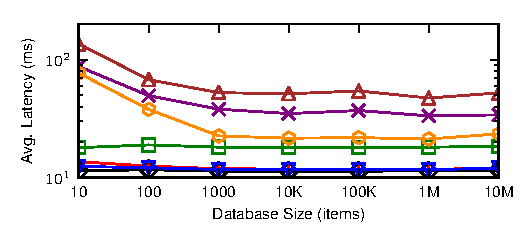
\includegraphics[width=\textwidth]{figs/numkeys-lat.pdf}
\end{minipage}
\end{center}
\caption{Comparison of algorithms for default parameters, sweeping one
  parameter per experiment}
\label{fig:comparison}

\end{figure*}
\end{comment}

\FloatBarrier
\subsection{Experimental Results: CTP Overhead} 
\label{sec:ctp}

We also evaluated the overhead of blocked writes in our implementation
of the Cooperative Termination Protocol discussed in
Section~\ref{sec:replication}. To simulate blocked writes, we
artificially dropped a percentage of \textsc{commit} commands in
\textsc{put\_all} calls such that clients returned from writes early
and partitions were forced to complete the commit via CTP. This
behavior is worse than expected because ``blocked'' clients continue
to issue new operations. The table below reports the throughput
reduction as the proportion of blocked writes increases (compared to
no blocked writes) for a workload of 100\% \rapl write
transactions:
\begin{center}
\small 
\begin{tabular}{|l|c|c|c|c|}
\hline
\textbf{Blocked \%} & 0.01\% & 0.1\% & 25\% & 50\% \\\hline
{\textbf{Throughput}} & No change & 99.86\% & 77.53\% & 67.92\% \\\hline
\end{tabular}
\end{center}
As these results demonstrate, CTP can reduce throughput because each
commit check consumes resources (namely, network and CPU
capacity). However, CTP only performs commit checks in the event of
blocked writes (or time-outs; set to 5s in our experiments), so a modest
failure rate of $1$ in $1000$ writes has a limited effect. The higher
failure rates produce a near-linear throughput reduction but, in
practice, a blocking rate of even a few percent is likely indicative
of larger systemic failures. As Figure~\ref{fig:others} hints, the
effect of additional metadata for the participant list in \rapb and
\raps is limited, and, for our default workload of 5\% writes,
we observe similar trends but with throughput degradation of 10\% or
less across the above configurations. This validates our initial motivation
behind the choice of CTP: average-case overheads are small.

\subsection{Experimental Results: Scalability}



\begin{figure}[th!]
\begin{center}
\hspace{5mm}
\includegraphics[width=\defaultfigwidth]{figs/legend-scaleout.pdf}\vspace{-.5em}
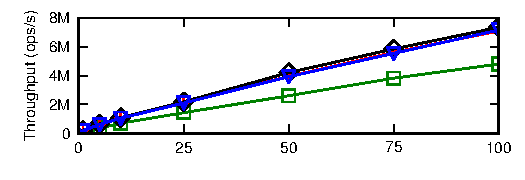
\includegraphics[width=.65\columnwidth]{figs/ns-thru.pdf}\vspace{-1.5em}
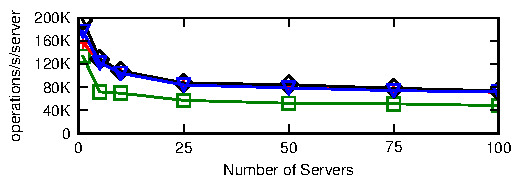
\includegraphics[width=.65\columnwidth]{figs/ns-perserver-thru.pdf}
\end{center}
\caption{RAMP transactions scale linearly to over $7$ million
  operations/s with comparable performance to \nwnr baseline.}
\label{fig:scaleout}
\end{figure}


We finally validate our chosen scalability criteria by demonstrating
linear scalability of RAMP transactions to 100 servers. We deployed an
increasing number of servers within the \texttt{us-west-2} EC2 region
and, to mitigate the effects of hot items during scaling, configured
uniform random access to items. We were unable to include more than 20
instances in an EC2 ``placement group,'' which guarantees 10 GbE
connections between instances, so, past 20 servers, servers
communicated over a degraded network. At around 40 servers, we
exhausted the \texttt{us-west-2b} ``availability zone'' (datacenter)
capacity and had to allocate our instances across the remaining zones,
further degrading network performance. To avoid bottlenecks on the
client, we deploy as many instances to host YCSB clients as we do to
host prototype servers.However, as shown in Figure~\ref{fig:scaleout},
each RAMP algorithm scales linearly. In expectation, at 100 servers,
almost all transactions span multiple servers: all but one in 100M
transactions is a multi-partition operation, highlighting the
importance of partition independence. With 100 servers, \rapl achieves
slightly under $7.1$ million operations per second, or 1.79 million
transactions per second on a set of 100 servers (71,635 operations
per partition per second). At all scales, \rapl throughput was always
within $10\%$ of \nwnr. With 100 servers, \rapl was within 2.6\%,
\raps within 3.4\%, and \raps was within 45\% of \nwnr. In light of
our scalability criteria, this behavior is unsurprising.

\FloatBarrier



\section{Applying and Modifying the RAMP Protocols}
\label{sec:ramp-application}

In this section, we discuss modifications to RAMP to enable multi-datacenter and efficient quorum replication as well as causally consistent operation. Our goals here are two-fold. First, we believe this section will be beneficial to systems implementers integrating RAMP protocols into databases such as Cassandra~\cite{cassandra-sigmod} that support wide-area and quorum-replicated deployments. Indeed, its inclusion is a reflection on many helpful reader comments asking for clarification on this topic. Second, we believe this material is a useful inclusion for readers who are familiar with existing and recent work on both multi-datacenter and causally consistent replication. Namely, RAMP is compatible with many of these replication scenarios, and, in some cases, enables new optimizations.

\subsection{Multi-Datacenter RAMP}
\label{sec:multidc}

The RAMP algorithms presented in this work have assumed linearizable server operation. Hence, if RAMP is used in a system where data items are replicated, then a linearizable replication mechanism must be used, such as a primary-backup or other replicated state machine approach. While this has simplified our discussion and results in reasonable performance in many environments, the cost of linearizability is often be expensive, particularly in geo-replicated environments where latency is lower-bounded by the speed of light~\cite{hat-vldb,pacelc}. While the RAMP algorithms' lack of coordination mitigates throughput penalties due to, for example, stalls during contended multi-partition access, actually accessing the partitions themselves may take time and increase the latency of individual operations. Moreover, in the event of partial failures, it is often beneficial to provide greater availability guarantees.

In this section, we discuss strategies for lowering the latency and improving the availability of operations. Our primary target in this setting is a multi-datacenter, geo-replicated context, where servers are located in separate clusters in possibly geographically remote regions. This setting has received considerable attention in recent research and, increasingly, in some of the largest production data management systems~\cite{walter,cops,eiger,spanner}. The actual porting of concurrency control algorithms to this context is not terribly difficult, but any inefficiencies due to synchronization and coordination are magnified in this setting, making it an idea candidate for practical study. Thus, we couch our discussion in the context of fully-replicated, geo-distributed clusters (i.e., groups of replicas of each partition).

The key challenge in achieving higher availability and lower latency in RAMP is ensuring that partially committed writes can still be completed. In the standard RAMP algorithms, this is accomplished by waiting to commit until after all partitions have prepared. Yet, in a replicated context, this waiting is potentially expensive; over wide-area networks, this can take hundreds of milliseconds. There are two straightforward ways to circumvent these overheads: deferring the commit operation and maintaining stickiness.


\begin{figure}[th!]
\begin{center}
\subfigure[High availability multi-cluster RAMP] {
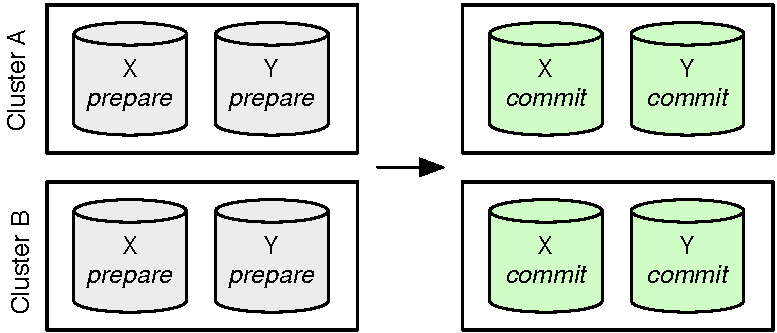
\includegraphics[width=.5\columnwidth]{diagram/mdc-ha.pdf}
\label{fig:mdc-ha}
}\\
\subfigure[Sticky multi-cluster RAMP] {
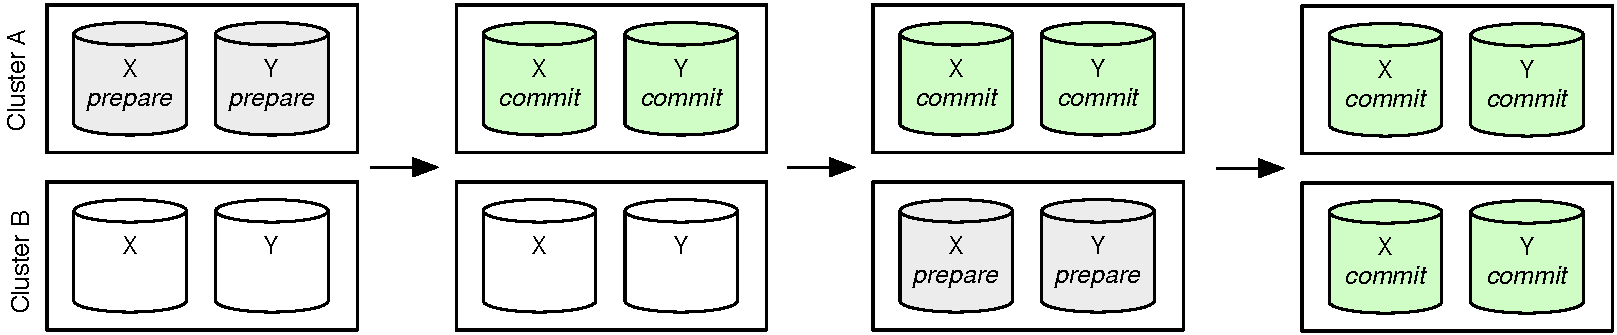
\includegraphics[width=\textwidth]{diagram/mdc-sticky.pdf}
\label{fig:mdc-sticky}
}\vspace{1em}

\caption{Control flow for operations under multi-datacenter RAMP strategies with client in Cluster A writing to partitions X and Y. In the high availability RAMP strategy (Figure~\ref{fig:mdc-ha}), a write must be prepared on $F+1$ servers (here, $F=3$) before is committed. In the sticky RAMP strategy, a write can be prepared and committed within a single datacenter and asynchronously propagated to other datacenters, where it is subsequently prepared and committed (Figure~\ref{fig:mdc-sticky}). The sticky strategy requires that clients maintain affinity with a single cluster in order to guarantee available and correctly isolated behavior.} 
 \end{center} \label{fig:mdc} \end{figure}


\minihead{\textit{Prepare-F HA RAMP}} The first strategy is easier to understand but perhaps less practical. A client specifies a minimum durability for its write operations, measured in terms of number of failures it wishes to survive, $F$. When writing, the client issues a prepare request to all clusters and waits until it receives a successful response from $F+1$ servers. This ensures that the client's write is durable, and the client knows its intent has been logged on at least $F+1$ servers. The client transaction subsequently returns success (Figure~\ref{fig:mdc-ha}). Once all servers have received the prepare request (which is detectable via either via server-server communication as in the CTP protocol or via an asynchronous callback on the client), the servers can begin to commit the client's writes autonomously. This preserves RA isolation---but at a cost. Namely, there is no guarantee of \textit{visibility} of writes: a client is not guaranteed to read its own writes. Moreover, if a single server is offline, the servers will not begin the commit step, and clients will not observe the effects of the prepared transactions for an indefinite period of time. By ensuring availability of writes (i.e., clients return early), we have sacrificed visibility in the form of ensuring that writes are accessible to readers. Thus, clients will not enjoy session guarantees~\cite{sessionguarantees} such as Read Your Writes. Given the importance of these session guarantees for many of the industrial users we have encountered (e.g., see Facebook's TAO geo-replication~\cite{tao}), we currently do not favor this approach.

\minihead{\textit{Sticky HA RAMP}} The second strategy is to ensure a degree of stickiness, or affinity, between clients and servers within a datacenter~\cite{hat-vldb}.  Each client is assigned its own datacenter.  Instead of having a client issue its writes to the entire database replica set, the client can instead issue its prepare and commit operations to its assigned datacenter (or local replica group) and subsequently forward the writes to be prepared and committed autonomously in separate clusters (Figure~\ref{fig:mdc-sticky}). That is, once a writer has performed the appropriate RAMP protocol in its assigned datacenter, it can return.  In an $N$-datacenter deployment, each full write protocol is performed $N$ separate times---once per datacenter. If the same timestamp is assigned to each write, the end state of each datacenter will be equivalent. As long as clients remain connected to the \textit{same} datacenter (i.e., is ``sticky'' with respect to its database connections), it will read its writes.

The total number of prepare and commit operations are the same as in the first strategy, but the commit point is staggered---each cluster reaches a commit point independently, at different times. Moreover, clusters operate independently, so throughput is not improved---only latency---because each cluster must replay every other cluster's writes~\cite{explicit-socc}. This is the basic strategy espoused by traditional log shipping approaches~\cite{lazyreplication} as well as more recent proposals such as the COPS~\cite{cops} and Eiger~\cite{eiger} systems.

However, this stickiness has an often-neglected penalty: a client can no longer connect to arbitrary servers and expect to read its own writes. If a server is down in a client's local datacenter, the client must---in the worst case---locate an entire other replica set to which the client can connect. This negatively affects availability: the \textit{Prepare-F} strategy can utilize all servers at once, but the sticky strategy requires clients to maintain affinity for availability. In cases when this ``sticky availability''~\cite{hat-vldb} is acceptable (e.g., each datacenter contains a set of application servers that issue the RAMP protocols against another datacenter-local set of storage servers), this may be a reasonable compromise.

\subsection{Quorum-Replicated RAMP Operation}
\label{sec:quorum}

 While RAMP \textit{Prepare-F} and \textit{Sticky HA} are best suited for multi-datacenter deployments, in quorum-replicated systems such as Dynamo and Cassandra~\cite{cassandra-sigmod,dynamo}, there are several optimizations that can be used to further improve availability, even within a single datacenter.

Our key observation here is that, to guarantee maximum of two-round trips for reads, only \textsc{prepare} and second-round \textsc{get} requests need to intersect on a given set of replicas. Recall that second-round \textsc{get} requests are issued in order to ``repair'' any fractured reads from the first round of read results. In the event of these fractured reads, a reader \textit{must} have access to versions corresponding to fractured reads that have been prepared but were not committed at the time of the first-round read. However, assembling the first round of committed versions can run under partial (i.e., non-intersecting) quorum operation~\cite{prob-quorum} with respect to commit messages.

This means that \textsc{commit} and first-round \textsc{get} operations can proceed on effectively any server in a set of replicas, enabling two key optimizations. In these optimizations, we assume that readers issue second-round read requests and writers issue \textsc{prepare} operations using a quorum system~\cite{naor-quorums} of replicas (e.g., majority quorums).

First, first-round read requests can be served from any replica of a given item. Then, if a client detects a race (in \rapl or \rapb), it can issue the optional second round of requests to a quorum of servers. \raps will always issue the second round of requests. This optimization improves the latency of the first round of reads and also enables speculative retry~\cite{tailscale}. It also decreases the load on the servers and increases availability for first-round read operations.

Second, commit operations can be performed on any replica of a given item. Similar to the optimization proposed in \textit{Prepare-F} RAMP, servers can propagate commit messages between themselves asynchronously, possibly piggybacking on anti-entropy messages as in systems like Cassandra and Dynamo. This optimization improves the latency of commit. However, because all servers must commit the transaction eventually, it does not necessarily decrease the load on servers.

To quantify the potential latency improvements achievable using these optimizations, we draw on latency distributions from a recent study of Dynamo-style operation~\cite{pbs-vldbj2013}. According to latency data from a Dynamo-style quorum-replicated database running on spinning disks at LinkedIn, moving from waiting for two replicas of three to respond to waiting for one replica of three to respond to a write request decreased latency from 21.0ms to 11.0ms at the 99.9th percentile; 1.63ms to 0.66ms for reads. For a similar database at Yammer, the gains for writes are 427ms to 10.8ms and the gains for reads are 32.6ms  to 5.6ms---an even more impressive gain. Over a wide-area network with latency of 75ms, the gains are as much as 148ms. Thus, in practice, these simple optimizations may prove worthwhile.

\subsection{RAMP, Transitive Dependencies, and Causal Consistency}
\label{sec:causal}

In Section~\ref{sec:ra-compare}, we discussed how RA isolation does not enforce transitive read-write dependencies across transactions. For example, if $T_a$ read-depends on $T_b$ (i.e., $T_a$ reads a version that $T_b$ created), another transaction $T_c$ might read-depend on $T_a$ (i.e., $T_c$ reads a version that $T_a$ created) but anti-depend on $T_b$ (i.e., $T_b$ overwrites a version that $T_a$ read). In this section, we discuss why we made this design decision as well as alternatives for enforcing dependencies and their costs.

% why did we do this?

The primary challenges in enforcing transitive dependencies come in limiting metadata while preserving availability and partition independence. In the extreme, if we limited ourselves to serial access to database state, we could easily preserve information about dependencies using a single scalar: any transactions would observe versions with lower scalar values, similar to classic serializable multi-version concurrency control. However, if we wish to preserve available and coordination-free operation (and therefore concurrent creation of versions), then we must admit a partial ordering of versions. To avoid fractured reads as in RA isolation while preserving dependency information, we either need to find a way to capture this partial order or otherwise limit the degree of availability in the system.

\minihead{Full causality tracking} The former approach---tracking ``cuts'' in a system with partially ordered events---is well-studied. As a first approximation, we can consider the problem of capturing RA with dependency tracking as an instance of capturing causality in a distributed system, with each event corresponding to a transaction commit and dependencies due to reads (i.e., a causal memory with atomically visible, multi-register reads). In line with this approximation, we could replace each timestamp in the RAMP algorithms with a suitable mechanism for tracking causality; for example, instead of storing a scalar timestamp, we could store a vector clock, with one entry per client in the system. Subsequently, clients could maintain a vector clock containing the highest-committed writes they had seen, and, upon reading from servers, ensure that the server commits any writes that happen-before the client's current vector. Thus, we can use vector clocks to track dependencies across transactions.

The problem with the above approach is in the size of the metadata required. Primarily, with $N$ concurrent clients, each vector will require $O(N)$ space, which is potentially prohibitive in practice. Moreover, the distributed systems literature strongly suggests that, with $N$ concurrent clients, $O(N)$ space is \textit{required} to capture full causal lineage as above~\cite{vc-lowerbound}. Thus, while using vector clocks to enforce transitive dependencies is a correct approach, it incurs considerable overheads that we do not wish to pay and have yet to be proven viable at scale in practical settings~\cite{explicit-socc}.\footnote{Another alternative that uses additional metadata is the strawman from Section~\ref{sec:sysmodel}, in which clients send all of the writes in their transaction to all of the partitions responsible for at least one write in the transaction. This uses even more metadata than the vector-based approach.}

The latter approach---limiting availability---is also viable, at the cost of undercutting our scalability goals from Section~\ref{sec:sysmodel}.

\minihead{Bounding writer concurrency} One simple approach---as we hinted above---is to limit the concurrency of writing clients: we can bound the overhead of vector clocks to an arbitrarily small amount by limiting the amount of concurrency in the system. For example, if we allow five clients to perform writes at a given time, we only need a vector of size five. This requires coordination between writers (but not readers). As Section~\ref{sec:eval-compare} demonstrated, RAMP transaction performance degrades gracefully under write contention; under the decreased concurrency strategy, performance would effectively hit a cliff. Latency would increase due to queuing delays and write contention, and, for a workload like YCSB with a fixed proportion of read to write operations, throughput would be limited. Specifically, for a workload with $p$ writers ($p=0.05$ in our default configuration), if $W$ writers were permitted at a given time, the effective number of active YCSB clients in the system would become $\frac{W}{p}$. Despite these limits, this is perhaps the most viable solution we have encountered and, moreover, does not affect read performance under read-heavy workloads. However, this solution has considerable coordination overheads, and managing which servers are able to perform writes (e.g., using distributed leases) requires potentially heavyweight synchronization protocols.

\minihead{Sacrificing partition independence} Another approach to improving availability is to sacrifice partition independence. As we discuss and evaluate in Sections~\ref{sec:setup} and~\ref{sec:eval-compare}, it is possible to preserve transaction dependencies by electing special coordinator servers as points of rendezvous for concurrently executing transactions. If extended to a non-partition-independent context, the RAMP protocols begin to more closely resemble traditional multi-version concurrency control solutions, in particular, Chan and Gray's read-only transactions~\cite{readonly}. More recently, the 2PC-PCI mechanism~\cite{eiger} we evaluated is an elegant means of achieving this behavior if partition independence is unimportant. Nevertheless, as our experimental evaluation shows, sacrificing this partition independence can be costly under some workloads.

\minihead{Sacrificing causality} A final approach to limiting the overhead of dependency tracking is to limit the number of dependencies to track. Several prior systems have used limited forms of causality, for example, application-supplied dependency information~\cite{bolton,lazyreplication}, as a basis for dependency tracking. In this strategy, applications inform the system about what versions should precede a given write; in~\cite{explicit-socc} (see also Section~\ref{sec:explicitcausality}), we show that, for many modern web applications, these histories can be rather small (often one item, with a power-law distribution over sizes). In this case, we could encode the causal history in its entirety along with each write or exploit otherwise latent information within the data such as comment \texttt{reply-to} fields to mine this data automatically. This strategy breaks the current RAMP API. However, it is the only known strategy for circumventing the $O(N)$ upper-bound on dependency tracking in causally consistent storage systems ensuring availability of both readers and writers.

\minihead{Experiences with system operators} While causal consistency provides a number of useful guarantees, in practice, we perceive a lack of interest in maintaining full causal consistency; database operators and users are anecdotally often unwilling to pay the metadata and implementation costs of full causality tracking. As we have seen in Section~\ref{sec:motivation}, many of these real-world operators exhibit an aversion to synchronization at scale, so maintaining availability is paramount to either their software offerings or business operation. In fact, we have anecdotally found coordination-free execution and partition independence to be valuable selling points for the RAMP algorithms presented in this work. Instead, we have found many users instead favor guarantees such as Read Your Writes (provided by the RAMP algorithms) rather than full dependency tracking, opting for variants of explicit causality (e.g., via foreign key constraints or explicit dependencies) or restricted, per-item causality tracking (e.g., version vectors~\cite{dynamo}). Despite this mild pessimism, we view further reduction of causality overhead to be an interesting area for future work---including a more conclusive answer to the availability-metadata trade-off surfaced by~\cite{vc-lowerbound}.


\FloatBarrier

\begin{comment}
\subsection{In Detail: Index Maintenance with RAMP}
\label{sec:index-detail}

In this section, we present additional detail about index maintenance with RAMP transactions. In our presentation of the RAMP thus far, we have largely concerned ourselves with opaque reads and writes to items defined by the user. In contrast, the writes required to perform index maintenance are \textit{not} opaque to the system and are well-defined (and often repetitive; e.g., of the form: ``update the index entry for value \textit{v} by adding ID \textit{i}''). Thus, in the case of index maintenance, we can exploit the structure of the data (as hinted in Section~\ref{sec:causal} to improve algorithm efficiency. We present details in two stages: performing insertions and updates, and issuing queries.

\minihead{Performing Insertions and Updates} When a base table is modified, the database system can automatically generate the appropriate set of updates to corresponding index entries to be applied as part of a RAMP write transaction upon transaction commit. If we represent indexes as a mapping from values (e.g., hair color) to a set of matching items (e.g., item and version), insertions generate an addition to a set, and deletions generate a deletion from a set.



\minihead{Issuing Queries}
\end{comment}



\chapter{Related Work}
\label{c.relatedwork}

In this chapter, we provide a discussion of related work. We begin
with a discussion of work related to the general themes in this
thesis, then examine specific areas in depth.


Database system designers have long sought to manage the trade-off
between consistency and coordination. As we have discussed,
serializability and its many implementations (including lock-based,
optimistic, and pre-scheduling
mechanisms)~\cite{silo,bernstein-book,tamer-book,hstore,gray-virtues,calvin,eswaran-consistency,sdd1}
are sufficient for maintaining application correctness. However,
serializability is not always necessary: serializable databases do not allow certain
executions that are correct according to application semantics.  This
has led to a large class of application-level---or
semantic---concurrency control models and mechanisms that admit
greater concurrency. There are several surveys on this topic, such
as~\cite{tamer-book,ic-survey}, and, in our solutions, we integrate
many concepts from this literature.

\minihead{Commutativity} One of the most popular alternatives to
serializability is to exploit \textit{commutativity}: if transaction
return values (e.g., of reads) and/or final database states are
equivalent despite reordering, they can be executed
simultaneously~\cite{weihl-thesis,kohler-commutativity,redblue}. Commutativity
is often sufficient for correctness but is not necessary. For example,
if an analyst at a wholesaler creates a report on daily cash flows,
any concurrent sale transactions will \textit{not} commute with the
report (the results will change depending on whether the sale
completes before or after the analyst runs her queries). However, the
report creation is \iconfluent with respect to, say, the invariant
that every sale in the report references a customer from the customers
table. \cite{kohler-commutativity,lamport-audit} provide additional
examples of safe non-commutativity.

\minihead{The CALM Theorem, Monotonicity, and Confluence}
Hellerstein's CALM Theorem~\cite{ameloot-calm} shows that program
outcomes are confluent, or deterministic, under coordination-free
execution if and only if the program logic is monotone. CALM is a
declarative result: it captures the class of computations that can be
implemented deterministically without coordination. CALM can also be
used as a program analysis technique: if a particular program
implementation uses only monotonic operations (where ``program'' could
include a service and its client code), then that program will be
deterministic when executed without coordination; otherwise,
coordination should be injected to ``protect'' non-monotonic
operations to ensure determinism.  CALM program analysis is natural to
apply in logic languages like Bloom~\cite{calm} where monotonicity can
be assessed from syntax.  It can also be applied to dataflow systems
like Storm~\cite{storm} with the help of program
annotations~\cite{blazes}.

CALM's notion of confluence differs from invariant confluence in
several ways. First, CALM assesses the confluence, or determinism, of
program logic; invariant confluence assesses whether a set of safety
properties holds during and following the execution of a set of
transactions over replicated or multi-versioned data given a
particular merge function. \Iconfluence admits non-deterministic
outcomes as long as the outcomes satisfy the provided invariants.
Second, CALM does not consider transactions, while invariant
confluence analyzes transactions that individually ensure
invariant-preserving updates.  Third, invariant confluence considers
replicated or multi-versioned state (via the use of the replica
abstraction). As discussed in Section~\ref{sec:model}, invariant
confluent does not distinguish between partially-replicated and
fully-replicated systems; under invariant confluence, a transaction is
presented with an entire logical snapshot (replica) of the database
upon which it can operate. A partially replicated implementation of a
set of \iconfluent operations may need to communicate with partitions
responsible for items that were not explicitly mentioned in the
transaction operations but that are related to invariants over data
modified by the transaction. Again, and by
Theorem~\ref{theorem:necessary}, for \iconfluent semantics, this
checking can be performed in parallel by concurrently committing
transactions over their respective logical replicas. However, in
contrast, CALM analysis is agnostic to replication, versioning, and
partitioning, which, if desired, are implemented as part of program
logic to be analyzed.

CALM and invariant confluence use different mathematical
foundations. CALM is based on monotonicity analysis from logic
programs. \Iconfluence generalizes classic partitioning arguments from
distributed systems to the domain of user-supplied invariants,
transactions, and merge functions. For associative, commutative, and
idempotent merge functions, an \iconfluent execution effectively
defines a join semi-lattice: invariants begin true in $D_0$ and remain
true as the execution progresses. Monotone programs also compute over
a join semi-lattice of relations and union. However, the analyses and
proof techniques of the two concepts are quite different.

Further understanding the relationship between invariant confluence
and CALM is an interesting area for exploration. For example, it is
natural to ask if there is an extension of CALM analysis that can,
like \iconfluence, incorporate invariants over possibly
non-deterministic outputs. A possible direction here is to view
invariants as boolean-valued formulas whose results ``start true'' and
monotonically remain true. In this direction, an invariant is a
morphism mapping from potentially monotone relational inputs to a
monotone boolean output lattice~\cite{blooml}.  Additionally, as CALM
is non-transactional and our formulation of invariant confluence is
inherently transactional, it is interesting to consider what
``transactional CALM'' would mean. In our formulation of \iconfluence,
transactions that violate invariants when committing to local replica
state are aborted; it is unclear how to model abort logic in CALM
analysis.

\minihead{Convergent Data Types} On a related subject, Commutative
Replicated Data Type (CRDT) objects~\cite{crdt} similarly ensure
convergent outcomes that reflect all updates made to each object.
This convergence is a useful \textit{liveness}
property~\cite{schneider-concurrent} (e.g., a converged CRDT OR-Set
reflects all concurrent additions and removals) but does not prevent
users from observing inconsistent data~\cite{redblue-new}, or
\textit{safety} (e.g., the CRDT OR-Set does not---by itself---enforce
invariants, such as ensuring that no employee belongs to two
departments), and are therefore not sufficient to guarantee
correctness for all applications. Here, we use CRDTs to implement many
of our merge functions, and we add safety to the intermediate states
and final outcomes. Thus, each replica state is, in effect, a CRDT,
and our goal is to determine which operations need coordination to
ensure variants of safety properties are upheld.

\minihead{Use of Invariants} A large number of database
designs---including, in restricted forms, many commercial databases
today---use various forms of application-supplied invariants,
constraints, or other semantic descriptions of valid database states
as a specification for application correctness
(e.g.,~\cite{korth-serializability,kemme-si-ic,garciamolina-semantics,ic-survey,ic-survey-two,decomp-semantics,redblue,homeostasis,davidson-survey,local-verification,redblue-new,rel-serial,pwsr-pods,tamer-tods}). We
draw inspiration and, in particular, our use of invariants from this
prior work. However, we are not aware of related work that discusses
when coordination is strictly \textit{required} to enforce a given set
of invariants. That is, our formulation of coordination-free execution
of transactions on separate replicas, which is key to capturing
scalability, low latency, and availability properties, is not found in
this related work; we, in effect, operate at the junction between this
prior work on semantics-based concurrency control from databases and
classic analyses from distributed
computing~\cite{gilbert-cap}. 

To illustrate why replication is so important to our model, consider
the work on relative serializability~\cite{rel-serial}. In this work,
the authors generalize prior efforts,
including~\cite{korth-serializability,garciamolina-semantics,atomictransactions,tamer-tods},
and re-define conflicting actions within otherwise conflict
serializable transaction execution in order to allow greater
concurrency. That is, instead of defining conflict as ``any two
operations on the same item from different transactions, at least one
of which is a write'' as in conflict serializability, relative
serializability allows users to define an abstract atomicity relation
to determine conflicts---for example, two increment operations need
not necessarily conflict, even if they both update the same
counter. Thus, the goal of this work is to preserve equivalence a
serial schedule, defined according to the abstract atomicity relation,
and there is still a total order on operations. As a result, in
relative serializability and related models~\cite{pwsr-pods}, the
``union'' (or combination) of two databases is undefined if two items
have different versions (e.g., $\{a_1\} \cup \{a_2\}$), because such
databases would correspond to two separate total orders. In contrast,
in our \iconfluence analysis, we explicitly consider a partial order
on operations, with divergent states reconciled with a merge operator;
instead of reasoning about conflicts, we allow arbitrary divergent
states that $i)$ are guaranteed to satisfy a user-specified invariant
over the data and $ii)$ are reconciled using a user-specified merge
function.

Because data is replicated in our model, it is natural to reason about
a ``merge'' function. Insofar as servers must explicitly integrate
updates from others in order to guarantee convergence (in contrast
with conventional shared-memory systems, where hardware automatically
chooses an ordering and conflict resolution policies for updates),
merge allows users to specify their own conflict resolution. As we
have discussed, the merge operator is itself drawn from the literature
on optimistic replication~\cite{optimistic} and is relatively popular
today in stores including Dynamo~\cite{dynamo} and its descendants as
well as systems like Git. Thus, while the goals of work on
semantics-based concurrency control (including relative
serializability) are similar to ours (especially in terms of
increasing concurrency), our use of merge leads to a substantially
different system and execution model. In effect, we can think of
\iconfluence as relative serializability with a special,
system-induced compensating action (``merge'') to deal with divergent
paths in the semantic serializability serialization graph (RSG), if
the graph were extended to account for replication.

Thus, our \iconfluence analysis here is inspired by prior work on
semantics-based concurrency control and adapts the practice of using
application (and database) criteria as the basis of concurrency
control to the replicated (and non-serializable, multi-versioned)
setting. Moreover, compared to this prior work, our practical focus
here is oriented towards invariants found in SQL and in modern
applications.

In contrast with many of the conditions above (esp. commutativity and
monotonicity), we explicitly require more information from the
application in the form of invariants (Kung and
Papadimitriou~\cite{kung1979optimality} suggest this is information is
\textit{required} for general-purpose non-serializable yet safe
execution.)  In this work, we provide a necessary and sufficient
condition for safe, coordination-free execution over replicated and
multi-version data. When invariants are unavailable, many of these
more conservative approaches may still be applicable. Our use of
analysis-as-design-tool is inspired by this literature---in
particular,~\cite{kohler-commutativity}.


\minihead{Coordination costs} In this work, we determine when
transactions can run entirely concurrently and without
coordination. In contrast, a large number of alternative models
(e.g.,~\cite{garciamolina-semantics,korth-serializability,isolation-semantics,local-verification,kemme-si-ic,aiken-confluence,laws-order})
assume serializable or linearizable (and therefore coordinated)
updates to shared state. These assumptions are standard (but not
universal~\cite{ec-txns}) in the concurrent programming
literature~\cite{schneider-concurrent,laws-order}. (Additionally,
unlike much of this literature, we only consider a single set of
invariants per database rather than per-operation invariants.) For
example, transaction chopping~\cite{chopping} and later
application-aware
extensions~\cite{decomp-semantics,agarwal-consistency} decompose
transactions into a set of smaller transactions, providing increased
concurrency, but in turn require that individual transactions execute
in a serializable (or strict serializable) manner.  This reliance on
coordinated updates is at odds with our goal of coordination-free
execution. However, these alternative techniques are useful in
reducing the duration and distribution of coordination once it is
established that coordination is required.

\minihead{Term rewriting} In term rewriting systems, \iconfluence
guarantees that arbitrary rule application will not violate a given
invariant~\cite{obs-confluence}, generalizing Church-Rosser
confluence~\cite{termrewriting}. We adapt this concept and effectively
treat transactions as rewrite rules, database states as constraint
states, and the database merge operator as a special \textit{join}
operator (in the term-rewriting sense) defined for all
states. Rewriting system concepts---including
confluence~\cite{aiken-confluence}---have previously been integrated
into active database systems~\cite{activedb-book} (e.g., in triggers,
rule processing), but we are not familiar with a concept analogous to
\iconfluence in the existing database literature.

\minihead{Coordination-free algorithms and semantics} Our work is
influenced by the distributed systems literature, where
coordination-free execution across replicas of a given data item has
been captured as ``availability''~\cite{gilbert-cap,queue}. A large
class of systems provides availability via ``optimistic replication''
(i.e., perform operations locally, then
replicate)~\cite{optimistic}. We---like others~\cite{ec-txns}---adopt
the use of the merge operator to reconcile divergent database
states~\cite{bayou} from this literature. Both traditional database
systems~\cite{adya} and more recent
proposals~\cite{redblue-new, redblue} allow the simultaneous use of
``weak'' and ``strong'' isolation; we seek to understand \textit{when}
strong mechanisms are needed rather than an optimal implementation of
either. Unlike ``tentative update'' models~\cite{sagas}, we do not
require programmers to specify compensatory actions (beyond merge,
which we expect to typically be generic and/or system-supplied) and do
not reverse transaction commit decisions. Compensatory actions could
be captured under \iconfluence as a specialized merge procedure.

The CAP Theorem~\cite{gilbert-cap,pacelc} recently popularized the
tension between strong semantics and coordination and pertains to a
specific model (linearizability). In a recent retrospective, Brewer
discusses the role of CAP in reasoning about and ``repairing'' more
general invariants, such as those we study
here~\cite{brewer-cap}. The relationship between serializability and
coordination requirements has also been well documented in the
database literature~\cite{davidson-survey}. Our research here
addresses when particular database-backed applications require
coordination, providing a new property, \iconfluence, for doing so.

\minihead{Summary} The \iconfluence property is a necessary and
sufficient condition for safe, coordination-free execution. Sufficient
conditions such as commutativity and monotonicity are useful in
reducing coordination overheads but are not always necessary. Here, we
explore the fundamental limits of coordination-free execution. To do
so, we explicitly consider a model without synchronous
communication. This is key to scalability: if, by default, operations
must contact a centralized validation service, perform atomic updates
to shared state, or otherwise communicate, then scalability will be
compromised. Finally, we only consider a single set of invariants for
the entire application, reducing programmer overhead without affecting
our \iconfluence results.



\subsubsection{Isolation and RAMP Transactions}

Replicated databases offer a broad spectrum of isolation guarantees at
varying costs to performance and availability~\cite{bernstein-book}:

\minihead{Serializability} At the strong end of the isolation spectrum
is serializability, which provides transactions with the equivalent of
a serial execution (and therefore also provides RA). A range of
techniques can enforce serializability in distributed
databases~\cite{bernstein-book,divy-writeonly}, multi-version
concurrency control (e.g.~\cite{mv-mobile}), locking
(e.g.~\cite{versions-update}), and optimistic concurrency
control~\cite{f1}. These useful semantics come with costs in the form
of decreased concurrency (e.g., contention and/or failed optimistic
operations) and limited availability during partial
failure~\cite{hat-vldb,davidson-survey}. Many
designs~\cite{hstore,gstore} exploit cheap serializability within a
single partition but face scalability challenges for distributed
operations. Recent industrial efforts like F1~\cite{f1} and
Spanner~\cite{spanner} have improved performance via aggressive
hardware advances but, their reported throughput is still limited to
20 and 250 writes per item per second. Multi-partition,
multi-datacenter, and, generally, distributed serializable
transactions are expensive and, especially under adverse conditions,
are likely to remain
expensive~\cite{schism,jones-dtxn,pavlo-partition}.

\minihead{Weak isolation} The remainder of the isolation spectrum is
more varied. Most real-world databases offer (and often default to)
non-serializable isolation models~\cite{mohan-note,hat-vldb}. These
``weak isolation'' levels allow greater concurrency and fewer
system-induced aborts compared to serializable execution but provide
weaker semantic guarantees. For example, the popular choice of
Snapshot Isolation prevents Lost Update anomalies but not Write Skew
anomalies~\cite{adya}; by preventing Lost Update,
concurrency control mechanisms providing Snapshot Isolation require coordination~\cite{hat-vldb}. In recent years, many
``NoSQL'' designs have avoided cross-partition transactions entirely,
effectively providing Read Uncommitted isolation in many industrial
databases such PNUTS~\cite{pnuts}, Dynamo~\cite{dynamo},
TAO~\cite{tao}, Espresso~\cite{espresso}, Rainbird~\cite{rainbird},
and BigTable~\cite{bigtable}. These systems avoid penalties associated
with stronger isolation but in turn sacrifice transactional guarantees
(and therefore do not offer RA).

%Swift~\cite{swift}, 

\minihead{RAMP and related mechanisms} There are several algorithms that are
closely related to our choice of RA and RAMP algorithm design.

COPS-GT's two-round read-only transaction protocol~\cite{cops} is
similar to \rapl reads---client read transactions identify causally
inconsistent versions by timestamp and fetch them from servers. While
COPS-GT provides causal consistency (requiring additional metadata),
it does not support RA isolation for multi-item writes.

Eiger provides its write-only transactions~\cite{eiger} by electing a
coordinator server for each write. As discussed in
Section~\ref{sec:ramp-evaluation} (\mstr), the number of ``commit checks''
performed during its read-only transactions is proportional to the
number of concurrent writes. Using a coordinator violates partition
independence but in turn provides causal consistency. This coordinator
election is analogous to G-Store's dynamic key grouping~\cite{gstore}
but with weaker isolation guarantees; each coordinator effectively
contains a partitioned completed transaction list
from~\cite{readonly}. Instead of relying on indirection, RAMP
transaction clients autonomously assemble reads and only require
constant factor (or, for \rapl, linear in transaction size) metadata
size compared to Eiger's \textit{PL-2L} (worst-case linear in database
size).

We are not aware of another concurrency control mechanism for
partitioned databases that ensures coordination-free execution,
partition independence, and at least RA isolation.

\subsubsection{Constraints}

There is a large body of related work related to our investigation of
specific database and ORM constraints that we consider in three
categories: object relational mapping systems, the quantification of
isolation behavior, and empirical open source software analysis.

\minihead{ORMs} Database systems and application programming
frameworks have a long
history~\cite{objectstore,shore,bernstein-orm}. The ``impedance
mismatch'' between object-oriented programming and the relational
model is a perennial problem in data management systems. Ruby on Rails
is no exception, and the concurrency control issues we study here are
endemic to this mismatch---namely, the disuse of common concurrency
control mechanisms like database-backed constraints. Bridging this gap
remains an active area of research~\cite{db-to-model}.

The latest wave of web programming frameworks has inspired diverse
research spanning databases, verification, and security. StatusQuo
uses program analysis and synthesis to transform imperative ORM code
into SQL, leveraging the efficiency of database-backed web
applications written in the Spring framework~\cite{statusquo}. Rails
has been the subject of study in the verification of cross-site
scripting attacks~\cite{rails-xss}, errors in data
modeling of associations~\cite{rails-bounded}, and arbitrary,
user-specified (non-validation) invariants~\cite{invariant-web}.
Rails-style ORM validations have been used to improve systems security
via client-side execution~\cite{waves,caveat}. Our focus here is on
the concurrency control requirements and usages of applications
written in Rails.

\minihead{Quantifying anomalies} A range of research similarly
quantifies the effect of non-serializable isolation in a variety of
ways.

Perhaps closest to our examination of ORM integrity violations is a
study by Fekete et al., which quantitatively analyzed data
inconsistencies arising from non-serializable
schedules~\cite{fekete-quantifying}. This study used a hand-crafted
benchmark for analysis but is nevertheless one of the only studies of
actual application inconsistencies. Here, we focus on open source
applications from the Rails community.

A larger body of work examines isolation anomalies at the read-write
interface (that is, measures deviations from properties such as
serializability or linearizability but \textit{not} the end effect of
these deviations on actual application behavior). Wada et
al. evaluated the staleness of Amazon's SimpleDB using end-user
request tracing~\cite{wada-data}, while Bermbach and Tai evaluated
Amazon S3~\cite{bermbach-eventual}, each quantifying various forms of
non-serializable behavior. Golab et al. provide algorithms for
verifying the linearizability of and sequential consistency arbitrary
data stores~\cite{golab-analyzing} and Zellag and Kemme provide
algorithms for verifying their
serializability~\cite{zellag-consistent} and other cycle-based
isolation anomalies~\cite{zellag-real}. As we have discussed,
Probabilistically Bounded Staleness provides time- and version-based
staleness predictions for eventually consistent data
stores~\cite{pbs}. Our focus here is on anomalies as observed by
application logic rather than read-write anomalies observed under weak
isolation.

\minihead{Empirical software analysis} Empirical software analysis of
open source software is a topic of active interest in the software
engineering research community~\cite{foss-icse}. In the parlance of
that community, in this work, we perform a mixed-methods analysis,
combining quantitative survey techniques with a confirmatory case
study of Rails's susceptibility to validation
errors~\cite{empiricalmethods}. In our survey, we attempt to minimize
sampling bias towards validation-heavy projects by focusing our
attention on popular projects, as measured by GitHub stars. Our use of
quantitative data followed by supporting qualitative data from
documentation and issue tracking---as well as the chronology of
methodologies we employed to attain the results presented here---can
be considered an instance of the sequential exploration
strategy~\cite{creswell2013research}. We specifically use these techniques in
service of better understanding use of database
concurrency control.



\newcommand{\transform}{\textsc{Transform}\xspace}

\section{RSIW Proof}

\label{sec:rsiwproof}


% total order valid because G1c is prohibited

To begin, we first show that there exists a well-defined total
ordering of write-only transactions in a history that is valid under
RA isolation. This will be useful in ordering write transactions in
our one-copy equivalent execution.

\begin{lemma}[Well-defined Total Order on Writes]
\label{lemma:to}
  Given a history $H$ containing read-only and write-only transactions
  that is valid under RA isolation, $DSG(H)$ does not contain any
  directed cycles consisting entirely of write-dependency edges.
\end{lemma}
\begin{proof}
  $H$ is valid under RA isolation and therefore does not exhibit
  phenomenon \textit{G1c}. Thus, $H$ does not contain any directed
  cycles consisting entirely of dependency edges. Therefore, $H$ does
  not contain any directed cycles consisting entirely of
  write-dependency edges.
\end{proof}

We will also need to place read-only transactions in our history. To
do so, we show that, under RA isolation and the RSIW property (i.e.,
the preconditions of Theorem~\ref{thm:rsw}), each read-only
transaction will only read from one write-only transaction.

\begin{lemma}[Single Read Dependency]
\label{lemma:onedep}
Given a history $H$ containing read-only and write-only transactions
that obeys the RSIW property and is valid under RA isolation, each
node in $DSG(H)$ contains at most one direct read-dependency edge.
\end{lemma}
\begin{proof}
  Consider a history $H$ containing read-only and write-only
  transactions that has RSIW and is valid under RA
  isolation. Write-only transactions have no reads, so they have no
  read-dependency edges in $DSG(H)$. However, suppose $DSG(H)$
  contained a node corresponding to a read-only transaction containing
  more than one direct read-dependency edge; call this read-only
  transaction $T_r$. For two read-dependency edges to exist, $T_r$
  must have read versions produced by at least two different
  write-only transactions; pick any two and call them $T_i$ and $T_j$,
  corresponding to read versions $x_a$ and $y_d$.

  If $x$ and $y$ are the same item, then $a < d$ or $d < a$. In either
  case, $T_r$ exhibits the fractured reads phenomenon and $H$ is not
  valid under RA isolation, a contradiction.

  Therefore, $x$ and $y$ must be distinct items. Because $H$ obeys the
  RSIW property, $T_r$ must also obey the RSIW property. By the
  definition of the RSIW property, $T_r$ must have only read items
  written to by $T_i$ and items also written to by $T_j$; this implies
  that $T_i$ and $T_j$ each wrote to items $x$ and $y$. We can label
  $T_i$'s write to $y$ as $y_b$ and $T_j$'s write to $x$ as $x_c$. Per
  Lemma~\ref{lemma:to}, $T_i$'s writes to $x$ and $y$ must either both
  come before or both follow $T_j$'s corresponding writes to $x$ and
  $y$ in the version order for each of $x$ and $y$; that is, either
  both $a < b$ and $c < d$ or both $b < a$ and $d < c$.

  If $a < b$ and $c < d$, then $T_r$ exhibits the fractured reads
  phenomenon: $T_r$ read $x_a$ and $y_d$ but $T_j$, which wrote $y_d$
  also wrote $x_b$, and $a < b$. If $b < a$ and $d < c$, then $T_r$
  again exhibits the fractured reads phenomenon: $T_r$ read $x_a$ and
  $y_d$ but $T_i$, which wrote $x_a$, also wrote $y_c$, and $d <
  c$. In either case, $H$ is not valid under RA isolation, a
  contradiction.

  Therefore, each node in $DSG(H)$ must not contain more than one
  read-dependency edge.
\end{proof}

We now use this ordering on reads and writes to construct a total
ordering on transactions in a history:

\begin{procedure}[Transform]
  Given a history $H$ containing read-only and write-only transactions
  that has RSIW and is valid under RA isolation,
  construct a total ordering $O$ of the transactions in $H$ as
  follows:
\begin{enumerate}
\item Perform a topological sorting in $O$ of committed write-only
  transactions in $H$ ordered by the write-dependency edges in
  $DSG(H)$. That is, for each pair of write-only transactions ($T_1$,
  $T_2$) in $H$ that performed at least one write to the same item,
  place the transaction that wrote the higher-versioned item later in
  $O$. Lemma~\ref{lemma:to} ensures such a total ordering exists.
\item For each committed read-only transaction $T_r$ in $H$, place
  $T_r$ in $O$ after the write-only transaction $T_w$ whose writes
  $T_r$ read (i.e., after the write-only transaction that $T_r$
  directly read-depends on) but before the next write-only transaction
  $T_{w'}$ in $O$ (or, if no such transaction exists, at the end of
  $O$). By Lemma~\ref{lemma:onedep}, each committed read-only
  transaction read-depends on only one write-only transaction, so this
  ordering is similarly well defined.
\end{enumerate}

Return $O$.

\end{procedure}

As an example, consider the following history:
\begin{eqnarray}
\label{hist:transform-example}
T_1 & w(x_1); w(y_1)\\
T_2 & w(x_2); w(y_2)\nonumber\\
T_3 & r(x_1); r(y_1)\nonumber\\
T_4 & r(y_2);\nonumber
\end{eqnarray}
History~\ref{hist:transform-example} obeys the RSIW property and is
also valid under RA isolation. Applying procedure~\transform to
History~\ref{hist:transform-example}, in the first step, we first
order our write-only transactions $T_1$ and $T_2$. Both $T_1$ and
$T_2$ write to $x$ and $y$, but $T_2$'s writes have a later version
number than $T_1$'s, so, according to Step 1 of~\transform, we have
$O=T_1; T_2$. Now, in Step 2 of~\transform, we consider the read-only
transactions $T_3$ and $T_4$. We place $T_3$ after the transaction
that it read from ($T_1$) and before the next write transaction in the
sequence ($T_2$), yielding $O=T_1; T_3; T_2$. We place $T_4$ after the
transaction that it read from ($T_2$) and, because there is no later
write-only transaction following $T_2$ in $O$, place $T_4$ at the end
of $O$, yielding $O=T_1; T_3; T_2; T_4$. In this case, we observe
that, as Theorem~\ref{thm:rsw} suggests, it is possible to~\transform
an RSIW and RA history into a one-copy serial equivalent and that $O$ is in fact
a one-copy serializable execution.

Now we can prove Theorem~\ref{thm:rsw}. We demonstrate that executing
the transactions of $H$ in the order resulting from
applying~\transform to $H$ on a single-copy database yields an
equivalent history (i.e., read values and final database state) as
$H$. Because $O$ is a total order, $H$ must be one-copy serializable.
\begin{proof}[Theorem~\ref{thm:rsw}]
  Consider history $H$ containing read-only and write-only
  transactions that has RSIW and is valid under RA
  isolation. We begin by applying~\transform to $H$ to produce an
  ordering $O$. 

  We create a new history $H_o$ by considering an empty one-copy
  database and examining each transaction $T_h$ in $O$ in serial order
  as follows: if $T_h$ is a write-only transaction, execute a new
  transaction $T_{ow}$ that writes each version produced by $T_h$ to
  the one-copy database and commits. If $T_h$ is a read-only
  transaction, execute a new transaction $T_{or}$ that reads from the
  sam items as $T_h$ and commits. $H_o$ is the result of a serial
  execution of transactions over a single logical copy of the
  database, $H_o$ is one-copy serializable.

  We now show that $H$ and $H_o$ are equivalent. First, all committed
  transactions and operations in $H$ also appear in $H_o$
  because~\transform operates on all transactions in $H$ and all
  transactions and their operations (with single-copy operations
  substituted for multi-version operations) appear in the total order
  $O$ used to produce $H_o$. Second, $DSG(H)$ and $DSG(H_o)$ have the
  same direct read dependencies. This is a straightforward consequence
  of Step 2 of~\transform: in $O$, each read-only transaction $T_r$
  appears immediately following the write-only transaction $T_w$ upon
  which $T_r$ read-depends. When the corresponding read transaction is
  executed against the single-copy database in $H_o$, the serially
  preceding write-only transaction will produce the same values that
  the read transaction read in $H$. Therefore, $H$ and $H_o$ are equivalent.

  Because $H_o$ is one-copy serializable and $H_o$ is equivalent to $H$, $H$
  must also be one-copy serializable.
\end{proof}

We have opted for the above proof technique because we believe
the~\transform procedure provides clarity into \textit{how} executions
satisfying both RA isolation and the RSIW property relate to their
serializable counterparts. An alternative and elegant proof approach
leverages the work on multi-version serializability
theory~\cite{bernstein-book}, which we sketch here. Given a
history $H$ that exhibits RA isolation and has RSIW, we show
that $MVSG(H)$ is acyclic. By an argument resembling
Lemma~\ref{lemma:onedep}, the in-degree for read-only transactions in
$SG(H)$ (i.e., Adya's direct read dependencies) is one. By an argument
resembling Lemma~\ref{lemma:to}, the edges between write-only
transactions in $MVSG(H)$ produced by the first condition of the
$MVSG$ construction ($x_i \ll x_j$ in the definition of the
$MVSG$~\cite[p. 152]{bernstein-book}; i.e., Adya's write dependencies)
are acyclic. Therefore, any cycles in the $MVSG$ must include at least
one of the second kind of edges in the $MVSG(H)$ ($x_j \ll x_i$; i.e.,
Adya's direct anti-dependencies). But, for such a cycle to exist, a
read-only transaction $T_r$ must anti-depend on a write-only
transaction $T_{wi}$ that in turn write-depends on another write-only
transaction $T_{wj}$ upon which $T_r$ read-depends. Under the RSIW
property, $T_{wi}$ and $T_{wj}$ will have written to at least one of
the same items, and the presence of a write-dependency cycle will
indicate a fractured reads anomaly in $T_r$.

\section{RAMP Correctness and Independence}

\label{sec:rampproofs}


\minihead{RAMP-F Correctness} To prove \rapl provides RA isolation, we
show that the two-round read protocol returns a transactionally atomic
set of versions. To do so, we formalize criteria for atomic (read)
sets of versions in the form of \textit{companion sets}. We will call
the set of versions produced by a transaction \textit{sibling
  versions} and say that $x$ is a sibling item to a write $y_j$ if
there exists a version $x_k$ that was written in the same transaction
as $y_j$.

Given two versions $x_i$ and $y_j$, we say that $x_i$ is a
\textit{companion version} to $y_j$ if $x_i$ is a transactional
sibling of $y_j$ or $x$ is a sibling item of $y_j$ and $i > j$. We say
that a set of versions $V$ is a \textit{companion set} if, for every
pair $(x_i, y_j)$ of versions in $V$ where $x$ is a sibling item of
$y_j$, $x_i$ is a companion to $y_j$. In
Figure~\ref{fig:rapl-execution}, the versions returned by $T_2$'s
first round of reads ($\{x_1, y_\bot\}$) do not comprise a companion
set because $y_\bot$ has a lower timestamp than $x_1$'s sibling
version of $y$ (that is, $x_1$ has sibling version $y_1$ and but $\bot
< 1$ so $y_\bot$ has too low of a timestamp). Subsets of companion
sets are also companion sets and companion sets also have a useful
property for RA isolation:
\begin{claim}[Companion sets are atomic]
\label{claim:companion-atomic}
In the absence of G1c phenomena, companion sets do not contain fractured reads.
\end{claim}

Claim~\ref{claim:companion-atomic} follows from the definitions of
companion sets and fractured reads.

\begin{proof}
If $V$ is a companion set, then
every version $x_i \in V$ is a companion to every other version
$y_j \in V$ where $v_j$ contains $x$ in its sibling items. If $V$
contained fractured reads, $V$ would contain two versions $x_i,y_j$
such that the transaction that wrote $y_j$ also wrote a version $x_k$,
$i<k$. However, in this case, $x_i$ would not be a companion to
$y_j$, a contradiction. Therefore, $V$ cannot contain fractured reads.
\end{proof}

To provide RA, \rapl clients assemble a companion set for the
requested items (in $v_{latest}$), which we prove below:

\begin{claim}\rapl provides Read Atomic isolation.\end{claim}

\begin{proof}
\label{proof:rapl-ra}
Each write in \rapl contains information regarding its siblings, which
can be identified by item and timestamp. Given a set of \rapl
versions, recording the highest timestamped version of each item (as
recorded either in the version itself or via sibling metadata) yields
a companion set of item-timestamp pairs: if a client reads two
versions $x_i$ and $y_j$ such that $x$ is in $y_j$'s sibling items but
$i < j$, then $v_{latest}[x]$ will contain $j$ and not
$i$. Accordingly, given the versions returned by the first round of
\rapl reads, clients calculate a companion set containing versions of
the requested items. Given this companion set, clients check the
first-round versions against this set by timestamp and issue a second
round of reads to fetch any companions that were not returned in the
first round. The resulting set of versions will be a subset of the
computed companion set and will therefore also be a companion
set. This ensures that the returned results do not contain fractured
reads. \rapl first-round reads access $lastCommit$, so each
transaction corresponding to a first-round version is committed, and,
therefore, any siblings requested in the (optional) second round of
reads are also committed. Accordingly, \rapl never reads aborted or
non-final (intermediate) writes. Moreover, \rapl timestamps are
assigned on a per-transaction basis, preventing write-dependency
cycles and therefore \textit{G1c}. This establishes that \rapl
provides RA\@.
\end{proof}

\minihead{RAMP-F Scalability and Independence} \rapl also provides the
independence guarantees from Section~\ref{sec:sysmodel}. The
following invariant over $lastCommit$ is core to \rapl \textsc{get}
request completion:
\begin{invariant}[Companions present]
\label{inv:suitable-present}

If a version $x_i$ is referenced by $lastCommit$ (that is,
$lastCommit[x] = i$), then each of $x_i$'s sibling versions are
present in $versions$ on their respective partitions.

\end{invariant}
Invariant~\ref{inv:suitable-present} is maintained by \rapl's
two-phase write protocol. $lastCommit$ is only updated once a
transaction's writes have been placed into $versions$ by a first round
of \textsc{prepare} messages. Siblings will be present in $versions$
(but not necessarily $lastCommit$).

\begin{claim}\rapl is coordination-free.\end{claim}

Recall from Section~\ref{sec:sysmodel} that coordination-free execution ensures that one client's
transactions cannot cause another client's to block and that, if a
client can contact the partition responsible for each item in its
transaction, the transaction will eventually commit (or abort of its
own volition).

\begin{proof}
Clients in \rapl do not communicate or coordinate with one another and
only contact servers. Accordingly, to show that \rapl provides
coordination-free execution, it suffices to show that server-side
operations always terminate. \textsc{prepare} and \textsc{commit}
methods only access data stored on the local partition and do not
block due to external coordination or other method invocations;
therefore, they complete. \textsc{get} requests issued in the first
round of reads have $ts_{req} = \bot$ and therefore will return the
version corresponding to $lastCommit[k]$, which was placed into
$versions$ in a previously completed \textsc{prepare}
round. \textsc{get} requests issued in the second round of client
reads have $ts_{req}$ set to the client's calculated
$v_{latest}[k]$. $v_{latest}[k]$ is a sibling of a version returned
from $lastCommit$ in the first round, so, due to
Invariant~\ref{inv:suitable-present}, the requested version will be
present in $versions$. Therefore, \textsc{get} invocations are
guaranteed access to their requested version and can return without
waiting. The success of \rapl operations does not depend on the success
or failure of other clients' \rapl operations.
\end{proof}

\begin{claim}\rapl provides partition independence.\end{claim}
\begin{proof}
\rapl transactions do not access partitions that are unrelated to each transaction's
specified data items and servers do not contact other servers in
order to provide a safe response for operations.
\end{proof}

\minihead{RAMP-S Correctness} \raps writes and first-round reads proceed
identically to \rapl writes, but the metadata written and returned is
different. Therefore, the proof is similar to \rapl, with a slight
modification for the second round of reads.

\begin{claim}\raps provides Read Atomic isolation.\end{claim}
\begin{proof}
  To show that \raps provides RA, it suffices to show that \raps
  second-round reads ($resp$) are a companion set. Given two versions
  $x_i, y_j \in resp$ such that $x \neq y$, if $x$ is a sibling item
  of $y_j$, then $x_i$ must be a companion to $y_j$. If $x_i$ were not
  a companion to $y_j$, then it would imply that $x$ is not a sibling
  item of $y_j$ (so we are done) or that $j > i$. If $j > i$, then,
  due to Invariant~\ref{inv:suitable-present} (which also holds for
  \raps writes due to identical write protocols), $y_j$'s sibling is
  present in $versions$ on the partition for $x$ and would have been
  returned by the server (line~\ref{raps-get-server-withts-end}), a
  contradiction. Each second-round \textsc{get} request returns only
  one version, so the final set of reads does not exhibit fractured reads.
\end{proof}

\minihead{RAMP-S Scalability and Independence} \raps ensures
coordination-free execution and partition independence. The proofs
closely resemble those of \rapl: Invariant~\ref{inv:suitable-present}
ensures that incomplete commits do not stall readers, and all
server-side operations are guaranteed to complete.

\minihead{RAMP-H Correctness} The probabilistic behavior of the \rapb Bloom
filter admits false positives. However, given unique transaction
timestamps (Section~\ref{sec:additional}), requesting false siblings
by timestamp and item does not affect correctness:

\begin{claim}\rapb provides Read Atomic isolation.\end{claim}
\begin{proof}
To show that \rapb provides Read Atomic isolation, it suffices to show
that any versions requested by \rapb second-round reads that would not
have been requested by \rapl second-round reads (call this set
$v_{false}$) do not compromise the validity of \rapb's returned
companion set. Any versions in $v_{false}$ do not exist: timestamps
are unique, so, for each version $x_i$, there are no versions $x_j$ of
non-sibling items with the same timestamp as $x_i$ (i.e., where
$i=j$). Therefore, requesting versions in $v_{false}$ do not change
the set of results collected in the second round.
\end{proof}


\minihead{RAMP-H Scalability and Independence} \rapb provides
coordination-free execution and partition independence. We omit full
proofs, which closely resemble those of \rapl. The only significant
difference from \rapl is that second-round \textsc{get} requests may
return $\bot$, but, as we showed above, these empty responses
correspond to false positives in the Bloom filter and therefore do not
affect correctness.




\section{Discussion}

Given our experiences designing and evaluating the RAMP transaction
protocols, we believe there are a number of interesting extensions
that merit further examination.

First, RAMP metadata effectively encodes a limited form of transaction
\textit{intent}: readers and servers are only able to repair fractured
reads because the metadata encodes the remainder of the work required
to complete the transaction. We believe it would be interesting to
generalize this concept to arbitrary program logic: for example, in a
model such as lazy transactions~\cite{lazytxn} or eventual
serializability~\cite{eventual-serial}, with transactions expressed as
stored procedures, multiple, otherwise conflicting/coordinating
clients could instead cooperate in order to complete one anothers'
transactions in the event of a failure---without resorting to the use
of a centralized master (e.g., for pre-scheduling or validating transaction
execution). This programming model is largely incompatible with
traditional interactive transaction execution but is nevertheless
exciting to consider as an extension of these protocols.

Second, and more concretely, we see several opportunities to extend
RAMP to more specialized use cases. The RAMP protocol family is
currently not well-suited to large scans and, as we have discussed,
does not enforce transitive dependencies across transactions. We view
restricting the concurrency of writers (but not readers) to be a
useful step forward in this area, with predictable impact on writer
performance. This strikes a middle ground between traditional MVCC and
the current RAMP protocols.

Finally, as we noted in Section~\ref{sec:ra-serializable}, efficient
transaction processing often focuses on weakening semantics (e.g.,
weak isolation) or changing the programming model (e.g., stored
procedures as above). As our investigation of the RSW property
demonstrates, there may exist compelling combinations of the two that
yield more intuitive, high-performance, or scalable results than
examining semantics or programming models in isolation. Addressing
this question is especially salient for the many users of weak
isolation models in practice today~\cite{hat-vldb}, as it can help
understand when applications require stronger semantics and when, in
fact, weak isolation is not simply fast but is also ``correct.''

\section{Summary}
\label{sec:conclusion}

This chapter described how to achieve atomically visible multi-partition
transactions without incurring the performance and availability
penalties of traditional algorithms. We first identified a new
isolation level---Read Atomic isolation---that provides atomic
visibility and matches the requirements of a large class of real-world
applications. We subsequently achieved RA isolation via scalable,
contention-agnostic RAMP transactions. In contrast with techniques
that use inconsistent but fast updates, RAMP transactions provide
correct semantics for applications requiring secondary indexing,
foreign key constraints, and materialized view maintenance while
maintaining scalability and performance. By leveraging
multi-versioning with a variable but small (and, in two of three
algorithms, constant) amount of metadata per write, RAMP transactions
allow clients to detect and assemble atomic sets of versions in one to
two rounds of communication with servers (depending on the RAMP
implementation). The choice of coordination-free and partition
independent algorithms allowed us to achieve near-baseline performance
across a variety of workload configurations and scale linearly to 100
servers. While RAMP transactions are not appropriate for all
applications, the many applications for which they are appropriate will
benefit significantly.




\chapter{Coordination Avoidance for Database Constraints}
\label{c.constraints}

Thus far, we have considered semantics expressed in terms of isolation
models and application programming patterns such as indexing. Both of
these specifications were relatively low-level. The first relied on
admissible read-write interleavings of transactions. The latter relied
on a bespoke isolation level that we introduced to exactly capture the
semantics of several existing scenarios that arise in databases and applications. In this chapter, we raise
the level of abstraction further and consider the use of
\textit{constraints}, or arbitrary user-defined predicates over
database state. We focus on constraints found in contemporary SQL and
Ruby on Rails applications.

As we discuss, these constraints are found in many database-backed
applications today. The constraints are not necessarily a full
specification of program correctness yet are frequently found in
modern applications (and are typically enforced by coordination). As candidates
for study, we draw upon popular constraints found in languages like
SQL as well as a range of constraints found in open source
applications, which we subsequently analyze for \iconfluence. As
before, we find that many are \iconfluent and provide
coordination-avoiding implementations of each.

\section{\IConfluence of SQL Constraints}
\label{sec:bcc-practice}
\label{sec:merge}

We begin our study of practical constraints by considering several
features of SQL, ending with abstract data types. We will apply these
results to full applications in Section~\ref{sec:evaluation}.

In this section, we focus on providing intuition and informal
explanations of our \iconfluence analysis. Interested readers can find
a more formal analysis in Section~\ref{sec:ic-constraints}.
including discussion of invariants not presented here. For convenience,
we reference specific proofs from Section~\ref{sec:ic-constraints} inline.


\begin{table}
\definecolor{yesgray}{gray}{0.92}
\begin{center}
\small
\begin{tabular}{|l|l|c|c|}
\hline
\textbf{Invariant} & \textbf{Operation} & \iconfluent? & Proof \#\\\hline

\rowcolor{yesgray}
Attribute Equality & Any & Yes &1\\
\rowcolor{yesgray}
Attribute Inequality & Any & Yes&2 \\
Uniqueness & Choose specific value & No&3\\
\rowcolor{yesgray}
Uniqueness & Choose some value & Yes&4\\
\texttt{AUTO\_INCREMENT} & Insert & No&5\\
\rowcolor{yesgray}
Foreign Key & Insert & Yes&6\\
Foreign Key & Delete & No&7\\
\rowcolor{yesgray}
Foreign Key & Cascading Delete & Yes&8\\
\rowcolor{yesgray}
Secondary Indexing & Update & Yes &9\\
\rowcolor{yesgray}
Materialized Views & Update & Yes &10\\\hline\hline
\rowcolor{yesgray}
> & Increment [Counter] & Yes &11 \\
< & Increment [Counter] & No &12\\
> & Decrement [Counter] & No &13\\
\rowcolor{yesgray}
< & Decrement [Counter] & Yes &14\\
\rowcolor{yesgray}
\texttt{[NOT] CONTAINS} & Any [Set, List, Map] & Yes &15, 16\\ 
\texttt{SIZE=} & Mutation [Set, List, Map] & No &17\\ \hline
\end{tabular}
\end{center}\vspace{-.5em}
\caption{Example SQL (top) and ADT \iconfluence along with
  references to formal proofs in Section~\ref{sec:ic-constraints}.}
\label{table:invariants}
\end{table}

\subsection{\IConfluence for SQL Relations}

We begin by considering several constraints found in SQL.

\minihead{Equality} As a warm-up, what if an application wants to
prevent a particular value from appearing in a database? For example,
our payroll application from Section~\ref{sec:motivation} might
require that every user have a last name, marking the \texttt{LNAME}
column with a \texttt{NOT NULL} constraint. While not particularly
exciting, we can apply \iconfluence analysis to insertions and updates
of databases with (in-)equality constraints (Claims 1, 2 in
Section~\ref{sec:ic-constraints}). Per-record inequality invariants are
\iconfluent, which we can show by contradiction: assume two database
states $S_1$ and $S_2$ are each $I$-$T$-reachable under per-record
in-equality invariant $I_e$ but that $I_e(S_1 \sqcup S_2)$ is
false. Then there must be a $r \in S_1 \sqcup S_2$ that violates $I_e$
(i.e., $r$ has the forbidden value). $r$ must appear in $S_1$, $S_2$,
or both. But, that would imply that one of $S_1$ or $S_2$ is not
$I$-valid under $I_e$, a contradiction.

\minihead{Uniqueness} We can also consider common uniqueness
invariants (e.g., \texttt{PRIMARY KEY} and \texttt{UNIQUE}
constraints). For example, in our payroll example, we wanted user IDs
to be unique. In fact, our earlier discussion in
Section~\ref{sec:motivation} already provided a counterexample showing
that arbitrary insertion of users is not \iconfluent under these
invariants: $\{$Stan:5$\}$ and $\{$Mary:5$\}$ are both
$I$-$T$-reachable states (Section~\ref{sec:ic-defs}) that can be
created by a sequence of insertions (starting at $S_0=\{\}$), but
their merge---$\{$Stan:5, Mary:5$\}$---is not $I$-valid. Therefore,
uniqueness is not \iconfluent for inserts of unique values (Claim
3). However, reads and deletions are both \iconfluent under uniqueness
invariants: reading and removing items cannot introduce duplicates.

Can the database safely \textit{choose} unique values on behalf of
users (e.g., assign a new user an ID)? In this case, we can achieve
uniqueness without coordination---as long as we have a notion of
replica membership (e.g., server or replica IDs). The difference is
subtle (``grant this record this specific, unique ID'' versus ``grant
this record some unique ID''), but, in a system model
with membership (as is practical in many contexts), is powerful. If
replicas assign unique IDs within their respective portion of the ID
namespace, then merging locally valid states will also be globally
valid (Claim 4).

\minihead{Foreign Keys} We can consider more complex invariants, such
as foreign key constraints. In our payroll example, each employee
belongs to a department, so the application could specify a constraint
via a schema declaration to capture this relationship (e.g.,
\texttt{EMP.D\_ID FOREIGN KEY REFERENCES DEPT.ID}).

Are foreign key constraints maintainable without coordination? Again,
the answer depends on the actions of transactions modifying the data
governed by the invariant. Insertions under foreign key constraints
\textit{are} \iconfluent (Claim 6). To show this, we again attempt to find two
$I$-$T$-reachable states that, when merged, result in invalid
state. Under foreign key constraints, an invalid state will contain a
record with a ``dangling pointer''---a record missing a corresponding
record on the opposite side of the association. If we assume there
exists some invalid state $S_1 \sqcup S_2$ containing a record $r$
with an invalid foreign key to record $f$, but $S_1$ and $S_2$ are
both valid, then $r$ must appear in $S_1$, $S_2$, or both. But, since
$S_1$ and $S_2$ are both valid, $r$ must have a corresponding foreign
key record ($f$) that ``disappeared'' during merge. Merge (in the
current model) does not remove versions, so this is impossible.

From the perspective of \iconfluence analysis, foreign key constraints
concern the \textit{visibility} of related updates: if individual
database states maintain referential integrity, a non-destructive
merge function such as set union cannot cause tuples to ``disappear''
and compromise the constraint. This also explains why models such as
read committed~\cite{adya} and read
atomic~\cite{adya} isolation as well as causal
consistency~\cite{hat-vldb} are also achievable without coordination:
simply restricting the visibility of updates in a given transaction's
read set does not require coordination between concurrent operations.

Deletions and modifications under foreign key constraints are more
challenging. Arbitrary deletion of records is unsafe: a user might be
added to a department that was concurrently deleted (Claim
7). However, performing cascading deletions (e.g., SQL \texttt{DELETE
  CASCADE}), where the deletion of a record also deletes \textit{all}
matching records on the opposite end of the association, is
\iconfluent under foreign key constraints (Claim 8). We can generalize
this discussion to updates (and cascading updates).

\minihead{Materialized Views} Applications often pre-compute results
to speed query performance via a materialized view~\cite{tamer-book}
(e.g., \texttt{UNREAD\_CNT} as \texttt{SELECT}\texttt{
}\texttt{COUNT(*)}\texttt{ }\texttt{FROM}\texttt{
}\texttt{emails}\texttt{ }\texttt{WHERE}\texttt{ }\texttt{read\_date =
  NULL}). We can consider a class of invariants that specify that
materialized views reflect primary data; when a transaction (or merge
invocation) modifies data, any relevant materialized views should be
updated as well. This requires installing updates at the same time as
the changes to the primary data are installed (a problem related to
maintaining foreign key constraints). However, given that a view
only reflects primary data, there are no ``conflicts.'' Thus,
materialized view maintenance updates are \iconfluent (Claim 10).

\subsection{\IConfluence for SQL Data Types}

So far, we have considered databases that store growing sets of
immutable versions. We have used this model to analyze several useful
constraints, but, in practice, databases do not (often) provide these
semantics, leading to a variety of interesting anomalies. For example,
if we implement a user's account balance using a ``last writer wins''
merge policy~\cite{crdt}, then performing two concurrent withdrawal
transactions might result in a database state reflecting only one
transaction (a classic example of the Lost Update
anomaly)~\cite{adya,hat-vldb}. To avoid variants of these
anomalies, many optimistic, coordination-free database designs have
proposed the use of \textit{abstract data types} (ADTs), providing
merge functions for a variety of uses such as counters, sets, and
maps~\cite{crdt,atomictransactions,weihl-thesis,blooml} that ensure
that all updates are reflected in final database state. For example, a
database can represent a simple counter ADT by recording the number of
times each transaction performs an \texttt{increment} operation on the
counter~\cite{crdt}.

\Iconfluence analysis is also applicable to these ADTs and their
associated invariants. For example, a row-level ``greater-than''
(\texttt{>}) threshold invariant is \iconfluent for counter
\texttt{increment} and \texttt{assign} ($\gets$) but not
\texttt{decrement} (Claims 11, 13), while a row-level ``less-than''
(\texttt{<}) threshold invariant is \iconfluent for counter
\texttt{decrement} and \texttt{assign} but not \texttt{increment}
(Claims 12, 14). This means that, in our payroll example, we can
provide \cfree support for concurrent salary increments but not
concurrent salary decrements. ADTs (including lists, sets, and maps)
can be combined with standard relational constraints like materialized
view maintenance (e.g., the ``total salary'' row should contain the
sum of employee salaries in the \texttt{employee} table).  This
analysis presumes user program explicitly use ADTs, and, as with our
generic set-union merge, \iconfluence ADT analysis requires a
specification of the ADT merge behavior (Section~\ref{sec:ic-constraints}
provides several examples).

\subsection{SQL Discussion and Limitations}

We have analyzed a number of combinations of invariants and operations
(shown in Table~\ref{table:invariants}). These results are by no
means comprehensive, but they are expressive for many applications
(Section~\ref{sec:evaluation}). In this section, we discuss lessons from this
classification process.

\minihead{Analysis mechanisms} We have manually analyzed particular
invariant and constraint combinations, demonstrating each to be
\iconfluent or not. To study actual SQL-based applications, we can
apply these labels via simple static analysis. Specifically, given
invariants (e.g., captured via SQL DDL) and transactions (e.g.,
expressed as stored procedures), we can examine each invariant and
each operation within each transaction and identify pairs that we have
labeled as \iconfluent or non-\iconfluent. Any pairs labeled as
\iconfluent can be marked as safe, while, for soundness (but not
completeness), any unrecognized operations or invariants can be
flagged as potentially non-\iconfluent. Despite its simplicity (both
conceptually and in terms of implementation), this technique---coupled
with the results of Table~\ref{table:invariants}---is sufficiently
powerful to automatically characterize the I-confluence of the
applications we consider in Section~\ref{sec:evaluation} when
expressed in SQL (with support for multi-row aggregates like Invariant
8 in Table~\ref{table:tpcc-invariants}).

By growing our recognized list of \iconfluent pairs on an as-needed
basis (via manual analysis of the pair), the above technique has
proven useful---due in large part to the common re-use of invariants
like foreign key constraints. However, one could use more complex
forms of program analysis. For example, one might analyze the
\iconfluence of \textit{arbitrary} invariants, leaving the task of
proving or disproving \iconfluence to an automated model checker or
SMT solver. While \iconfluence---like monotonicity and commutativity
(Chapter~\ref{c.relatedwork})---is undecidable for arbitrary
programs, others have recently shown this alternative approach (e.g.,
in commutativity analysis~\cite{kohler-commutativity,redblue-new} and
in invariant generation for view serializable
transactions~\cite{homeostasis}) to be fruitful for restricted
languages. We view language design and more automated analysis as an
interesting area for future work (Section~\ref{sec:c-futurework}).

\minihead{Recency and session support} Our proposed invariants are
declarative, but a class of useful semantics---recency, or real-time
guarantees on reads and writes---describe properties of operations
(i.e., they pertain to transaction execution rather than the state(s)
of the database). For example, users often wish to read data that is
up-to-date as of a given point in time (e.g., ``read
latest''~\cite{pnuts} or linearizable~\cite{gilbert-cap}
semantics). While traditional isolation models do not directly address
these recency guarantees~\cite{adya}, they are often important to
programmers. Are these models \iconfluent? We can attempt to simulate
recency guarantees in \iconfluence analysis by logging the result of
all reads and any writes with a timestamp and requiring that all
logged timestamps respect their recency guarantees (thus treating
recency guarantees as invariants over recorded read/write execution
traces). However, this is a somewhat pointless exercise: it is well
known (and we have already discussed) that recency guarantees are
unachievable with transactional
availability~\cite{hat-vldb,gilbert-cap,davidson-survey}. Thus, if
application reads face these requirements, coordination is
required. Indeed, when application ''consistency'' means ``recency,''
systems cannot circumvent speed-of-light delays.

If users wish to ``read their writes'' or desire stronger ``session''
guarantees~\cite{bayou} (e.g., maintaining recency on a per-user or
per-session basis), they must maintain affinity or
``stickiness''~\cite{hat-vldb} with a given (set of) replicas. These
guarantees are also expressible in the \iconfluence model and do
not require coordination between different users' or sessions'
transactions.


\section{More Formal \IConfluence Analysis of SQL Constraints}
\label{sec:ic-constraints}

In this section, we more formally demonstrate the \iconfluence of
invariants and operations discussed in Section~\ref{sec:merge}. Our
goals in this section are two-fold. First, we have found the
experience of formally proving \iconfluence to be instructive in
understanding these combinations (beyond less formal arguments made in
the body text for brevity and intuition). Second, we have found
\iconfluence proofs to take on two general structure typically take
one of two forms:

\begin{itemize}

\item To show a set of transactions are not \iconfluent with respect to an invariant $I$, we use proof by counterexample: we present two $I$-$T$-reachable states with a common ancestor that, when merged, are not $I$-valid. 

\item To show a set of transactions are \iconfluent with respect to an
  invariant $I$, we use proof by contradiction: we show that, if a
  state $S$ is not $I$-valid, merging two $I$-$T$-reachable states
  $S_1$ and $S_2$ with a common ancestor state to produce $S$ implies
  either one or both of $S_1$ or $S_2$ must not be $I$-valid.

\end{itemize}

These results are not exhaustive, and there are literally infinite combinations of invariants and operations to consider. Rather, the seventeen examples below serve as a demonstration of what can be accomplished via \iconfluence analysis.

Notably, the negative results below use fairly simple histories
consisting of a single transaction divergence. Nevertheless, we
decided to preserve the more general formulation of \iconfluence
(accounting for arbitrary $I$-$T$-reachable states) to account for
more pathological (perhaps less realistic, or, if these results are
any indication, less commonly encountered) behaviors that only arise
during more complex divergence patterns.

We introduce additional formalism as necessary. To start, unless
otherwise specified, we use the set union merge operator. We denote
version $i$ of item $x$ as $x_i$ and a write of version $x_i$ with
value $v$ as $w(x_i=v)$. For now, we assume each version has an
integer value.

\begin{claim}[Writes are \iconfluent with respect to per-item equality constraints]
\label{claim:eq-proof}
Assume writes are not \iconfluent with respect to some per-item equality constraint $i=c$, where $i$ is an item and $c$ is a constant. By definition, there must exist two $I$-$T$-reachable states $S_1$ and $S_2$ with common ancestor state such that $I(S_1) \rightarrow true$ and $I(S_2) \rightarrow true$ but $I(S_1 \sqcup S_2) \rightarrow false$; therefore, there exists a version $i_n$ in $S_1 \sqcup S_2$ such that $i_n \neq c$, and, under set union, $i_n \in S_1$, $i_n \in S_2$, or both. However, this would imply that $I(S_1) \rightarrow false$ or $I(S_2) \rightarrow false$ (or both), a contradiction.
\end{claim} 

\begin{claim}[Writes are \iconfluent with respect to per-item inequality constraints] \label{claim:neq} The proof follows almost identically to the proof of Claim~\ref{claim:eq-proof}, but for an invariant of the form $i\neq c$.  \end{claim}

\begin{claim}[Writing arbitrary values is not \iconfluent with respect to multi-item uniqueness constraints]
\label{claim:sunique}
Consider the following transactions:
\begin{align*}
T_{1u}&\coloneqq w(x_a=v);~commit\\
T_{2u}&\coloneqq w(x_b=v);~commit
\end{align*}
and uniqueness constraint on records:
$$I_u(D) = \{\textrm{values of versions in D are unique}\}$$
Now, an empty database trivially does not violate uniqueness constraints ($I_u(D_s=\{\})\rightarrow true$), and adding individual versions to the separate empty databases is also valid:
\begin{align*}
T_{1u}(\{\})&=\{x_a=v\},~I_u(\{x_a=v\}) \rightarrow true\\
T_{2u}(\{\})&=\{x_b=v\},~I_u(\{x_b=v\}) \rightarrow true
\end{align*}
However, merging these states results in invalid state:
$$I_u(\{x_a=v\}\sqcup \{x_b=v\} = \{x_a=v, x_b=v\}) \rightarrow false$$
Therefore, $\{T_{1u}, T_{2u}\}$ is not \iconfluent under $I_s$.
\end{claim} 

For the next proof, we consider a model as suggested in
Section~\ref{sec:bcc-practice} where replicas are able to generate
unique (but not arbitrary (!)) IDs (in the main text, we suggested the
use of a replica ID and sequence number). In the following proof, to
account for this non-deterministic choice of unique ID, we introduce a
special $nonce()$ function and require that, $nonce()$ return unique
values for each replica; this can be achieved by assigning each replica a
unique ID and implementing nonce by returning the ID along with a local sequence number. That is, $\sqcup$ is not defined for replicas
on which independent invocations of $nonce()$ return the same value.

\begin{claim}[Assigning values by $nonce()$ is \iconfluent with respect to multi-item uniqueness constraints]
\label{claim:nunique}

Assume that assigning values by $nonce()$ is not \iconfluent with respect to some multi-item uniqueness invariant:
$$I(D) = \forall c \in dom(D), \{|\{x \in D \mid x = c\}| \leq 1 \}$$
By definition, there must exist two $I$-$T$-reachable states with a common ancestor reached by executing nonce-generating transactions (of the form $T_i=[w(x_i = nonce())]$), $S_1$ and $S_2$ such that $I(S_1) \rightarrow true$ and $I(S_2) \rightarrow true$ but $I(S_1 \sqcup S_2) \rightarrow false$.

Therefore, there exist two versions $i_a, i_b$ in $S_1 \sqcup S_2$ such that $i_a$ and $i_b$ (both generated by $nonce()$) are equal in value. Under set union, this means $i_a \in S_1$ and $i_b \in S_2$ ($i_a$ and $i_b$ both cannot appear in $S_1$ or $S_2$ since it would violate those states' $I$-validity). Because replica states grow monotonically under set merge and $S_1$ and $S_2$ differ, they must be different replicas. But $nonce()$ cannot generate the same values on different replicas, a contradiction. \end{claim}

\begin{claim}[Writing arbitrary values are not \iconfluent with respect to sequentiality constraints]
\label{claim:nseq-insert}
Consider the following transactions:
\begin{align*}
T_{1s}&\coloneqq w(x_a=1);~commit\\
T_{2s}&\coloneqq w(x_b=3);~commit
\end{align*}
and the sequentiality constraint on records:
$$I_s(D) =\{max(r\in D)-min(r\in D) = |D|+1\} \vee \{|D|=0\}$$
Now, $I_s$ holds over the empty database ($I_s(\{\}) \rightarrow true$), while inserting sequential new records into independent, empty replicas is also valid:
\begin{align*}
T_{1s}(\{\})&=\{x_a=1\},~I_u(\{x_a=1\}) \rightarrow true\\
T_{2s}(\{\})&=\{x_b=3\},~I_u(\{x_b=3\}) \rightarrow true
\end{align*}
However, merging these states results in invalid state:
$$I_s(\{x_a=1\}\sqcup \{x_b=3\} = \{x_a=1, x_b=3\}) \rightarrow false$$
Therefore, $\{T_{1s}, T_{2s}\}$ is not \iconfluent under $I_s$.
\end{claim}

To discuss foreign key constraints, we need some way to \textit{refer}
to other records within the database. There are a number of ways of
formalizing this. Here, refer to a field $f$ within a given version
$x_i$ as $x_i.f$. In the following discussion, recall that
\iconfluence analysis is performed on fully replicated sets of
data. While there is considerable \textit{implementation} complexity
involved in actually performing multi-partition foreign key constraint
maintenance (and indexing; as in RAMP) this is not germane to our
model. As a simple strawman solution, we can defer all calculation of
tombstoned records until writes have quiesced, guaranteeing
convergence. As a slightly more advanced strawman, we can calculate
tombstoned records according to a global watermark of writes that is
advanced via background consensus.

\begin{claim}[Insertion is \iconfluent with respect to foreign key constraints]
\label{claim:fk-insert}
  Assume that inserting new records is not \iconfluent with respect to some foreign key constraint $I(D) = \{\forall r_f \in D$ such that $r_f.g \neq null$, $\exists r_t \in D$ such that $r_f.g = r_t.h\}$ (there exists a foreign key reference between fields $g$ and $h$). By definition, there must exist two $I$-$T$-reachable states $S_1$ and $S_2$ with a common ancestor reachable by executing transactions performing insertions such that $I(S_1) \rightarrow true$ and $I(S_2) \rightarrow true$ but $I(S_1 \sqcup S_2) \rightarrow false$; therefore, there exists some version $r_1 \in S_1 \sqcup S_2$ such that $r_1.g \neq null$ but $\nexists r_2 \in S_1 \sqcup S_2$ such that $r_1.g = r_2.h$. Under set union, $r_1$ must appear in either $S_1$ or $S_2$ (or both), and, for each set of versions in which it appears, because $S_1$ and $S_2$ are both $I$-valid, they must contain an $r_3$ such that $r_1.f = r_3.h$. But, under set union, $r_3.h$ should also appear in $S_1 \sqcup S_2$, a contradiction.
\end{claim}

For simplicity, in the following proof, we assume that deleted elements remain deleted under merge. In practice, this can be accomplished by tombstoning records and, if required, using counters to record the number of deletions and additions~\cite{crdt}. We represent a deleted version $x_d$ by $\neg x_b$.

\begin{claim}[Concurrent deletion and insertion is not \iconfluent with respect to foreign key constraints]
\label{claim:fk-delete}
 Consider the following transactions:
\begin{align*}
T_{1f}&\coloneqq w(x_a.g=1);~commit\\
T_{2f}&\coloneqq delete(x_b);~commit
\end{align*}
and the foreign key constraint:
$$I_f(D) = \{\forall r_f \in D, r_f.g \neq null,~\exists r_t \in D \suchthat \neg r_t \notin D \mathand r_f.g = r_t.h\}$$
Foreign key constraints hold over the initial database $S_i=\{x_b.h=1\}$ ($I_u(S_i) \rightarrow true$) and on independent execution of $T_a$ and $T_b$:
\begin{align*}
T_{1f}(\{x_b.h=1\})&=\{x_a.g=1, x_b.h=1\},~I_f(\{x_a=1\}) \rightarrow true\\
T_{2f}(\{x_b.h=1\})&=\{x_b.h=1, \neg {x_b}\}~I_f(\{x_b.h=1, \neg {x_b}\}) \rightarrow true
\end{align*}
However, merging these states results in invalid state: 
$$I_f(\{x_a.g=1\}\sqcup \{x_b.h=1, \neg {x_b}\}) \rightarrow false$$
Therefore, $\{T_{1f}, T_{2f}\}$ is not \iconfluent under $I_f$.\end{claim}

We denote a cascading delete of all records that reference field $f$ with value $v$ ($v$ a constant) as $cascade(f=v)$.

\begin{claim}[Cascading deletion and insertion are \iconfluent with respect to foreign key constraints]
\label{claim:fk-cascade}
Assume that cascading deletion and insertion of new records are not \iconfluent with respect to some foreign key constraint $I(D) = \{\forall r_f \in D$ such that $r_f.g \neq null$, $\exists r_t \in D$ such that $r_f.g = r_t.h$ if $cascade(h=r_f.g \neq v)\}$ (there exists a foreign key reference between fields $g$ and $h$ and the corresponding value for field $h$ has not been deleted-by-cascade). By definition, there must exist two $I$-$T$-reachable states $S_1$ and $S_2$ with common ancestor reachable by performing insertions such that $I(S_1) \rightarrow true$ and $I(S_2) \rightarrow true$ but $I(S_1 \sqcup S_2) \rightarrow false$; therefore, there exists some version $r_1 \in S_1 \sqcup S_2$ such that $r_1.f \neq null$ but $\nexists r_2 \in S_1 \sqcup S_2$ such that $r_1.g = r_2.h$. From the proof of Claim~\ref{claim:fk-insert}, we know that insertion is \iconfluent, so the absence of $r_2$ must be due to some cascading deletion. Under set union, $r_1$ must appear in exactly one of $S_1$ or $S_2$ (if $r_1$ appeared in both, there would be no deletion, a contradiction since we know insertion is \iconfluent). For the state $S_j$ in which $r_1$ does not appear (either $S_1$ or $S_2$), $S_j$ must include $cascade(h=r_1.g)$. But, if $cascade(h=r_1.g) \in S_j$, $cascade(h=r_1.g)$ must also be in $S_i \sqcup S_j$, a contradiction and so $S_i \sqcup S_j \rightarrow true$, a contradiction.
\end{claim}

We define a ``consistent'' secondary index invariant as requiring that, when a record is visible, its secondary index entry should also be visible. This is similar to the guarantees provided by Read Atomic isolation~\cite{ramp-sigmod14}. For simplicity, in the following proof, we only consider updates to a single indexed attribute $attr$, but the proof is easily generalizable to multiple index entries, insertions, and deletion via tombstones. We use last-writer wins for index entries.

\begin{claim}[Updates are \iconfluent with respect to consistent secondary indexing] \label{claim:indexing}
  Assume that updates to records are not \iconfluent with respect a secondary index constraint on attribute $attr$:

\noindent $I(D) = \{\forall r_f \in D$ such that $r_f.attr \neq null$ and $f$ is the highest version of $r\in D$, $\exists r_{idx} \in D$ such that $r_f \in r_{idx}.entries$ (all entries with non-null $attr$ are reflected in the secondary index entry for $attr$).

  Represent an update to record $r_x$ as $\{w(r_x)$ and, if $r_x.attr \neq null$, also $r_{idx}.entries.add(r_x)$, else $r_{idx}.entries.delete(r_x)\}$.

  By definition, there must exist two $I$-$T$-reachable states $S_1$ and $S_2$ with common ancestors reachable by performing insertions $S_1$ and $S_2$ such that $I(S_1) \rightarrow true$ and $I(S_2) \rightarrow true$ but $I(S_1 \sqcup S_2) \rightarrow false$; therefore, there exists some version $r_1 \in S_1 \sqcup S_2$ such that $r_1.attr \neq null$ but $\nexists r_{idx} \in S_1 \sqcup S_2$ or $\exists r_{idx} \in S_1 \sqcup S_2$ but $r_1 \notin r_{idx}.entries$. In the former case, $r_{idx} \notin S_1$ or $S_2$, but $r_1 \in S_1$ or $r_1 \in S_2$, a contradiction. The latter case also produces a contradiction: if $r_1 \in S_1$ or $r_1 \in S_2$, it must appear in $r_{idx}$, a contradiction.  \end{claim}

In our formalism, we can treat materialized views as functions over database state $f(D) \rightarrow c$.

\begin{claim}[Updates are \iconfluent with respect to materialized view maintenance] The proof is relatively straightforward if we treat the materialized view record(s) $r$ as having a foreign key relationship to any records in the domain of the function (as in the proof of Claim~\ref{claim:fk-cascade} and recompute the function on update, cascading delete, and $\sqcup$.\end{claim}

For our proofs over counter ADTs, we represent increments of a counter $c$ by $inc_i(c)$, where $i$ is a distinct invocation, decrements of $c$ by $dec_i(c)$, and the value of $c$ in database $D$ as $val(c, D) = |\{j \mid inc_j(c) \in D\}| - |\{k \mid dec_k(c) \in D\}|$.

\begin{claim}[Counter ADT increments are \iconfluent with respect to greater-than constraints] \label{claim:ge-inc-adt}
Assume increments are not \iconfluent with respect to some per-counter greater-than constraint $I(D)=val(c, D) < k$, where $k$ is a constant. By definition, there must exist two $I$-$T$-reachable states $S_1$ and $S_2$ with common ancestor reachable by executing write transactions such that $I(S_1) \rightarrow true$ and $I(S_2) \rightarrow true$ but $I(S_1 \sqcup S_2) \rightarrow false$; therefore, $val(c, S_1 \sqcup S_2) \leq k$. However, this implies that $val(c, S_1) \leq k)$, $val(c, S_2$, or both, a contradiction.  \end{claim}

\begin{claim}[Counter ADT increments are not \iconfluent with respect to less-than constraints]
\label{claim:le-inc-adt}
Consider the following transactions:
\begin{align*}
T_{1i}&\coloneqq inc_1(c);~commit\\
T_{2i}&\coloneqq inc_2(c);~commit
\end{align*}
and the less-than inequality constraint:
$$I_i(D) = \{val(c, D) < 2\}$$
$I_i$ holds over the empty database state ($I_i(\{\}) \rightarrow true$) and when $T_a$ and $T_b$ are independently executed:
\begin{align*}
T_{1i}(\{\})&=\{inc_1(c)=1\},~I_i(\{inc_1(c)=1\}) \rightarrow true\\
T_{2i}(\{\})&=\{inc_2(c)\},~I_i(\{inc_2(c)\}) \rightarrow true
\end{align*}
However, merging these states results in invalid state:
$$I_u(\{inc_1(c)\}\sqcup \{inc_2(c)\}) \rightarrow false$$
Therefore, $\{T_{1i}, T_{2i}\}$ is not \iconfluent under $I_u$.
\end{claim}

\begin{claim}[Counter ADT decrements are not \iconfluent with respect to greater-than constraints] The proof is similar to the proof of Claim~\ref{claim:le-inc-adt}; substitute $dec$ for $inc$ and choose $I_i(D) = \{val(c,D) > -2\}$.  \end{claim}

\begin{claim}[Counter ADT decrements are \iconfluent with respect to less-than constraints] \label{claim:le-inc-adt} Unsurprisingly, the proof is almost identical to the proof of Claim~\ref{claim:ge-inc-adt}, but with $<$ instead of $>$ and $dec$ instead of $inc$. \end{claim}

We provide proofs for ADT lists; the remainder are remarkably similar. Our implementation of ADT lists in these proofs uses a lexicographic sorting of values to determine list order. Transactions add a version $v$ to list $l$ via $add(v,l)$ and remove it via $del(v,l)$ (where an item is considered contained in the list if it has been added more times than it has been deleted) and access the length of $l$ in database $D$ via $size(l) = |\{k \mid add(k, l) \in D\}|- |\{m \mid del(m, l) \in D\}|$ (note that $size$ of a non-existent list is zero).

\begin{claim}[Modifying a list ADT is \iconfluent with respect to containment constraints]
  Assume ADT list modifications are not \iconfluent with respect to some equality constraint $I(D)=\{add(k, l) \in D \wedge del(k, l) \notin D \}$ for some constant $k$. By definition, there must exist two $I$-$T$-reachable states $S_1$ and $S_2$ with common ancestor reachable by list modifications such that $I(S_1) \rightarrow true$ and $I(S_2) \rightarrow true$ but $I(S_1 \sqcup S_2) \rightarrow false$; therefore, $add(k, l) \notin \{S_1 \sqcup S_2\}$ or $del(k, l) \in \{S_1 \sqcup S_2\}$. In the former case, neither $S_1$ nor $S_2$ contain $add(k,l)$ a contradiction. In the latter case, if either of $S_1$ or $S_2$ contains $del(k,l)$, it will be invalid, a contradiction.\end{claim}

\begin{claim}[Modifying a list ADT is \iconfluent with respect to non-containment constraints]
Assume ADT list modifications are not \iconfluent with respect to some non-containment constraint $I(D)=\{add(k, l) \notin D \wedge del(k, l) \in D\}$ for some constant $k$. By definition, there must exist two $I$-$T$-reachable states $S_1$ and $S_2$ with common ancestor reachable via list modifications such that $I(S_1) \rightarrow true$ and $I(S_2) \rightarrow true$ but $I(S_1 \sqcup S_2) \rightarrow false$; therefore, $add(k, l) \in \{S_1 \sqcup S_2\}$ and $del(k,l) \notin \{S_1 \sqcup S_2\}$. But this would imply that $add(k, l) \in S_1$, $add(k, l) \in S_2$, or both (while $del(k,l)$ is in neither), a contradiction.\end{claim}

\begin{claim}[Arbitrary modifications to a list ADT are not \iconfluent with respect to equality constraints on the size of the list]
Consider the following transactions:
\begin{align*}
T_{1l}&\coloneqq del(x_i, l);~add(x_a, l);~commit\\
T_{2l}&\coloneqq del(x_i, l);~add(x_b, l);~commit
\end{align*}
and the list size invariant:
$$I_l(D) = \{size(l) = 1\}$$
Now, the size invariant holds on a list of size one ($I_u(\{add(x_i, l)\}) \rightarrow true$) and on independent state modifications:
\begin{align*}
T_{1l}(\{add(x_i, l)\})&=\{add(x_i, l),~del(x_i, l),~add(x_a, l)\}\\
T_{2l}(\{add(x_i, l)\})&=\{add(x_i, l),~del(x_i, l),~add(x_b,1)\}
\end{align*}
However, merging these states result in an invalid state:
\begin{align*}
I_l(&\{add(x_i, l),~del(x_i, l),~add(x_a, l)\}\\\sqcup~&\{add(x_i, l),~del(x_i, l),~add(x_b, l)\})\rightarrow false
\end{align*}
Therefore, $\{T_{1l}, T_{2l}\}$ is not \iconfluent under $I_u$.
\end{claim}

Note that, in our above list ADT, modifying the list is \iconfluent with respect to constraints on the head and tail of the list but not intermediate elements of the list! That is, the head (resp. tail) of the merged list will be the head (tail) of one of the un-merged lists. However, the second element may come from either of the two lists.


\section{Empirical Impact: SQL-Based Constraints}
\label{sec:evaluation}

When achievable, coordination-free execution enables scalability
limited to that of available hardware. This is powerful: a
\iconfluent application can scale out without
sacrificing correctness, latency, or availability. In
Section~\ref{sec:bcc-practice}, we saw combinations of invariants
and transactions that were \iconfluent and others that were not. In this
section, we apply these combinations to the workloads of the
OLTP-Bench suite~\cite{oltpbench}, with a focus on the TPC-C
benchmark. Our focus is on the coordination required in order to
correctly execute each and the resulting, coordination-related
performance costs.

\subsection{TPC-C Invariants and Execution}
\label{sec:tpcc-invariants}

The TPC-C benchmark is the gold standard for database concurrency
control~\cite{oltpbench} both in research and in industry~\cite{tpcc},
and in recent years has been used as a yardstick for distributed
database concurrency control
performance~\cite{calvin,hstore,silo}. How much coordination does
TPC-C actually require a compliant execution?

The TPC-C workload is designed to be representative of a wholesale
supplier's transaction processing requirements. The workload has a number of
application-level correctness criteria that represent basic business
needs (e.g., order IDs must be unique) as formulated by the TPC-C
Council and which must be maintained in a compliant run. We can
interpret these well-defined ``consistency criteria'' as invariants and
subsequently use \iconfluence analysis to determine which transactions
require coordination and which do not.

Table~\ref{table:tpcc-invariants} summarizes the twelve invariants
found in TPC-C as well as their \iconfluence analysis results as
determined by Table~\ref{table:invariants}. We classify the invariants
into three broad categories: materialized view maintenance, foreign
key constraint maintenance, and unique ID assignment. As we discussed
in Section~\ref{sec:bcc-practice}, the first two categories are
\iconfluent (and therefore maintainable without coordination) because
they only regulate the \textit{visibility} of updates to multiple
records. Because these (10 of 12) invariants are \iconfluent under the
workload transactions, there exists some execution strategy that does
not use coordination. However, simply because these invariants are
\iconfluent does not mean that \textit{all} execution strategies will
scale well: for example, using locking would \textit{not} be
coordination-free.


\begin{table}[t!]
\definecolor{yesgray}{gray}{0.92}
\small
\begin{tabular}{|l|l|l|l|l|}
  \hline
  \textbf{\#} & \textbf{Informal Invariant Description} &
  \textbf{Type} & 
  \textbf{Txns} & \textbf{$\mathcal{I}$-C} \\\hline
  \rowcolor{yesgray}
  1 & {\scriptsize YTD wh sales = sum(YTD district sales)} & MV &
  P & Yes\\
  2 &  {\scriptsize Per-district order IDs are sequential} &$\mathrm{S_{ID}}$+FK  & N, D & No\\
  3 &  {\scriptsize New order IDs are sequentially assigned} & $\mathrm{S_{ID}}$  & N, D & No \\
  \rowcolor{yesgray}
  4 & {\scriptsize  Per-district, item order count = roll-up} & MV &
  N & Yes\\
  \rowcolor{yesgray}
  5 &  {\scriptsize Order carrier is set iff order is pending} & FK &
  N, D & Yes \\
  \rowcolor{yesgray}
  6 &  {\scriptsize Per-order item count = line item roll-up} & MV & N
  & Yes \\
  \rowcolor{yesgray}
  7 &  {\scriptsize Delivery date set iff carrier ID set} & FK & D & Yes \\
  \rowcolor{yesgray}
  8 &  {\scriptsize YTD wh = sum(historical wh)} & MV &
  D & Yes \\
  \rowcolor{yesgray}
  9 &  {\scriptsize YTD district = sum(historical district)} &
  MV & P & Yes \\
  \rowcolor{yesgray}
  10 &  {\scriptsize Customer balance matches expenditures} & MV & P, D & Yes \\
  \rowcolor{yesgray}
  11 &  {\scriptsize Orders reference New-Orders table}  & FK & N & Yes \\
  \rowcolor{yesgray}
  12 &  {\scriptsize Per-customer balance = cust. expenditures} & MV & P, D &
  Yes \\\hline

\end{tabular}
\caption{TPC-C Declared ``Consistency Conditions'' (3.3.2.x) and \iconfluence
  analysis results with respect to the workload transactions
  (Invariant type: MV: materialized view, $\mathbf{S_{ID}}$: sequential ID assignment, FK: foreign
  key; Transactions: N: New-Order, P: Payment, D: Delivery).}
\label{table:tpcc-invariants}
\end{table}


As one coordination-free execution strategy (which we implement in
Section~\ref{sec:evaltpcc}) that respects the foreign key and
materialized view invariants, we can use RAMP transactions from
Chapter~\ref{c.ramp}, which provide atomically visible transactional
updates across servers without relying on coordination for
correctness. As a reminder, RAMP transactions employ limited
multi-versioning and metadata to ensure that readers and writers can
always proceed concurrently: any client whose reads overlap with
another client's writes to the same item(s) can use metadata stored in
the items to fetch any ``missing'' writes from the respective
servers. A standard RAMP transaction over data items suffices to
enforce foreign key constraints, while a RAMP transaction over
commutative counters as described in~\cite{ramp-sigmod14} is sufficient to
enforce the TPC-C materialized view constraints.

Two of TPC-C's invariants are not \iconfluent with respect to the
workload transactions and therefore \textit{do} require
coordination. On a per-district basis, order IDs should be assigned
sequentially (both uniquely and sequentially, in the New-Order
transaction) and orders should be processed sequentially (in the
Delivery transaction). If the database is partitioned by warehouse (as
is standard~\cite{silo,calvin,hstore}), the former is a distributed
transaction (by default, $10\%$ of New-Order transactions span
multiple warehouses). The benchmark specification allows the latter to
be run asynchronously and in batch mode on a per-warehouse
(non-distributed) basis, so we, like others~\cite{calvin,silo}, focus
on New-Order. Including additional transactions like the read-only
Order-Status in the workload mix would increase performance due to the
transactions' lack of distributed coordination and (often
considerably) smaller read/write footprints.

\minihead{Avoiding New-Order Coordination} New-Order is not
\iconfluent with respect to the TPC-C invariants, so we can always
fall back to using serializable isolation. However, the per-district
ID assignment records (10 per warehouse) would become a point of contention,
limiting our throughput to effectively $\frac{100W}{RTT}$ for a
$W$-warehouse TPC-C benchmark with the expected $10\%$ distributed
transactions. Others~\cite{silo} (including us, in prior
work~\cite{hat-vldb}) have suggested disregarding consistency criteria
3.3.2.3 and 3.3.2.4, instead opting for unique but non-sequential ID
assignment: this allows inconsistency and violates the benchmark
compliance criteria.

During a compliant run, New-Order transactions must
coordinate. However, as discussed above, only the ID assignment
operation is non-\iconfluent; the remainder of the operations in the
transaction can execute coordination-free. With some effort, we can
avoid \textit{distributed }coordination. A na\"{\i}ve implementation might grab
a lock on the appropriate district's ``next ID'' record, perform
(possibly remote) remaining reads and writes, then release the lock at
commit time. Instead, as a more efficient solution, New-Order can
defer ID assignment until commit time by introducing a layer of
indirection. New-Order transactions can generate a temporary, unique,
but non-sequential ID (\texttt{tmpID}) and perform updates using this
ID using a RAMP transaction (which, in turn, handles the foreign key
constraints)~\cite{ramp-sigmod14}. Immediately prior to transaction
commit, the New-Order transaction can assign a ``real'' ID by
atomically incrementing the current district's local``next ID'' record
(yielding \texttt{realID}) and recording the \texttt{[tmpID, realID]}
mapping in a special ID lookup table. Any read requests for the
\texttt{ID} column of the Order, New-Order, or Order-Line tables can
be safely satisfied (transparently to the end user) by joining with
the ID lookup table on \texttt{tmpID}. In effect, the New-Order ID
assignment can use a nested atomic
transaction~\cite{atomictransactions} upon commit, and all
coordination between any two transactions is confined to a
single server.

\subsection{Evaluating TPC-C New-Order}
\label{sec:evaltpcc}


\begin{figure}
\hspace{1.5em}\includegraphics[width=.6\columnwidth]{figs/ca_serial_legend.pdf}
\includegraphics[width=.6\columnwidth]{figs/client_thru.pdf}
\includegraphics[width=.6\columnwidth]{figs/wh_thru.pdf}
\includegraphics[width=.6\columnwidth]{figs/remote_thru.pdf}\vspace{.5em}
%\includegraphics[width=\figscale\columnwidth]{figs/wh_thru_single.pdf}
\caption{TPC-C New-Order throughput across eight servers.}
\label{fig:clients}
\end{figure}


We subsequently implemented the above execution strategy in a
distributed database prototype to quantify the overheads associated
with coordination in TPC-C New-Order. Most notably, the
coordination-avoiding query plan scales linearly to over 12.7M
transactions per second on $200$ servers while substantially
outperforming distributed two-phase locking. Our goal here is to
demonstrate---beyond the microbenchmarks of
Section~\ref{sec:motivation}---that safe but judicious use of
coordination can have meaningful positive effect on performance.

\begin{comment}
We originally ported TPC-C
New-Order to our prior RAMP transaction prototype~\cite{ramp-sigmod14} but
found that the larger transaction footprint was poorly suited for the
threading model. Each New-Order transaction generates between 13--33
reads and 13--33 writes, so switching to an event-based RPC layer with
support for batching and connection pooling delivered an approximate
factor of two improvement in throughput, while additional optimization
(e.g., more efficient indexing, fewer object allocations) delivered
another factor of two. 
\end{comment}

\minihead{Implementation and Deployment} We employ a multi-versioned
storage manager, with RAMP-Fast transactions for snapshot reads and
atomically visible writes/``merge'' (providing a variant of regular
register semantics, with writes visible to later transactions after
commit)~\cite{ramp-sigmod14} and implement the nested atomic transaction
for ID assignment as a sub-procedure inside RAMP-Fast's server-side
commit procedure (using spinlocks). We implement transactions as
stored procedures and fulfill the TPC-C ``Isolation Requirements'' by
using read and write buffering as proposed in~\cite{hat-vldb}. As is
common~\cite{calvin,abadi-vll,hstore,jones-dtxn}, we disregard
per-warehouse client limits and ``think time'' to increase load per
warehouse. In all, our base prototype architecture is similar to that
of~\cite{ramp-sigmod14}: a JVM-based partitioned, main-memory, mastered
database.

For an apples-to-apples comparison with a coordination-intensive
technique within the same system, we also implemented textbook
two-phase locking (2PL)~\cite{bernstein-book}, which provides
serializability but also requires distributed coordination. We totally
order lock requests across servers to avoid deadlock, batching lock
requests to each server and piggybacking read and write requests on
lock request RPC. As a validation of our implementation, our 2PL
prototype achieves per-warehouse (and sometimes aggregate) throughput
similar to (and often in excess of) several recent serializable
database implementations (of both 2PL and other
approaches)~\cite{calvin,abadi-vll,hstore,jones-dtxn}.

By default, we deploy our prototype on eight EC2 \texttt{cr1.8xlarge}
instances (32 cores comprising 88 Amazon Elastic Compute units, each
with 244GB RAM) in the Amazon EC2 \texttt{us-west-2} region with
non-co-located clients and one warehouse per server (recall there
are 10 ``hot'' district ID records per warehouse) and report the
average of three 120 second runs.

\minihead{Basic behavior} Figure~\ref{fig:clients} shows performance
across a variety of configurations, which we detail below. Overall,
the coordination-avoiding query plan far outperforms the serializable
execution. The coordination-avoiding query plan performs some
coordination, but, because coordination points are not distributed
(unlike 2PL), physical resources (and not coordination) are the bottleneck.

\miniheadit{Varying load} As we increase the number of clients, the
coordination-avoiding query plan throughput increases linearly, while
2PL throughput increases to $40$K transactions per second, then levels
off. As in our microbenchmarks in
Section~\ref{sec:background-cmotivation}, the former utilizes
available hardware resources (bottlenecking on CPU cycles at $640$K
transactions per second), while the latter bottlenecks on logical
contention.

\miniheadit{Physical resource consumption} To understand the overheads
of each component in the coordination-avoiding query plan, we used JVM
profiling tools to sample thread execution while running at peak
throughput, attributing time spent in functions to relevant modules
within the database implementation (where possible):

\begin{center}
\centering
\small
\setlength{\fboxsep}{4pt}
\fbox{
\begin{tabular}{l r}
\textbf{Code Path} & \textbf{Cycles}\\
Storage Manager (Insert, Update, Read) & 45.3\%\\
Stored Procedure Execution & 14.4\%\\
RPC and Networking & 13.2\%\\
Serialization & 12.6\%\\
ID Assignment Synchronization (spinlock contention) & 0.19\%\\
Other & 14.3\%\\
\end{tabular}}
\end{center}

The coordination-avoiding prototype spends a large portion of
execution in the storage manager, performing B-tree modifications and
lookups and result set creation, and in RPC/serialization. In contrast
to 2PL, the prototype spends less than $0.2\%$ of time coordinating,
in the form of waiting for locks in the New-Order ID assignment; the
(single-site) assignment is fast (a linearizable integer increment and
store, followed by a write and fence instruction on the spinlock), so
this should not be surprising. We observed large throughput penalties
due to garbage collection (GC) overheads (up to 40\%)---an unfortunate
cost of our highly compact (several thousand lines of Scala),
JVM-based implementation. However, even in this current prototype,
physical resources are the bottleneck---not coordination.

\miniheadit{Varying contention} We subsequently varied the number of
``hot,'' or contended items by increasing the number of warehouses on
each server. Unsurprisingly, 2PL benefits from a decreased
contention, rising to over $87$K transactions per second with $64$
warehouses. In contrast, our coordination-avoiding implementation is
largely unaffected (and, at $64$ warehouses, is even negatively
impacted by increased GC pressure). The coordination-avoiding query
plan is effectively agnostic to read/write contention.

\miniheadit{Varying distribution} We also varied the percentage of
distributed transactions. The coordination-avoiding query plan
incurred a $29\%$ overhead moving from no distributed transactions to
all distributed transactions due to increased serialization overheads
and less efficient batching of RPCs. However, the 2PL implementation decreased in throughput by over $90\%$ (in line
with prior results~\cite{abadi-vll,calvin}, albeit exaggerated here
due to higher contention) as more requests stalled due to coordination
with remote servers.

\minihead{Scaling out} Finally, we examined our prototype's scalability,
again deploying one warehouse per server. As Figure~\ref{fig:scaleout}
demonstrates, our prototype scales linearly, to over 12.74 million
transactions per second on 200 servers (in light of our earlier
results, and, for economic reasons, we do not run 2PL at this
scale). Per-server throughput is largely constant after 100 servers,
at which point our deployment spanned all three \texttt{us-west-2}
datacenters and experienced slightly degraded per-server performance.
While we make use of application semantics, we are unaware of
any other compliant multi-server TPC-C implementation that has
achieved greater than 500K New-Order transactions per
second~\cite{calvin,jones-dtxn,hstore,abadi-vll}.

\minihead{Summary} We present these quantitative results as a proof of
concept that executing even challenging workloads like TPC-C that
contain complex integrity constraints are not necessarily at odds with
scalability if implemented in a coordination-avoiding
manner. Distributed coordination need not be a bottleneck for all
applications, even if conflict serializable execution indicates
otherwise. Coordination avoidance ensures that physical
resources---and not logical contention---are the system bottleneck
whenever possible.

\begin{figure}
\includegraphics[width=\figscale\columnwidth]{figs/scale_thru_total.pdf}
\includegraphics[width=\figscale\columnwidth]{figs/scale_thru_each.pdf}\vspace{.5em}
\caption{Coordination-avoiding New-Order scalability.}
\label{fig:scaleout}
\end{figure}

\subsection{Analyzing Additional Applications}

These results begin to quantify the effects of coordination-avoiding
concurrency control. If considering \textit{application-level}
invariants, databases only have to pay the price of coordination when
necessary. We were surprised that the ``current industry standard for
evaluating the performance of OLTP systems''~\cite{oltpbench} was so
amenable to coordination-avoiding execution---at least for compliant
execution as defined by the official TPC-C specification.

For greater variety, we also studied the workloads of the recently
assembled OLTP-Bench suite~\cite{oltpbench}, performing a similar
analysis to that of Section~\ref{sec:tpcc-invariants}. We found (and
confirmed with an author of~\cite{oltpbench}) that for nine of
fourteen remaining (non-TPC-C) OLTP-Bench applications, the workload
transactions did not involve integrity constraints (e.g., did not
modify primary key columns), one (\texttt{CH-benCHmark}) matched
TPC-C, and two specifications implied (but did not explicitly state) a
requirement for unique ID assignment (\texttt{AuctionMark}'s
\texttt{new-purchase} order completion, \texttt{SEATS}'s
\texttt{NewReservation} seat booking; achievable like TPC-C order
IDs). The remaining two benchmarks, \texttt{sibench} and
\texttt{smallbank} were specifically designed as research benchmarks
for serializable isolation. Finally, the three ``consistency
conditions'' required by the newer TPC-E benchmark are a proper subset
of the twelve conditions from TPC-C considered here (and are all
materialized counters). It is possible (even likely) that these
benchmarks are underspecified, but according to official
specifications, TPC-C contains the most coordination-intensive
invariants among all but two of the OLTP-Bench workloads.

Anecdotally, our conversations and experiences with real-world
application programmers and database developers have not identified
invariants that are radically different than those we have studied
here. A simple thought experiment identifying the invariants required
for a social networking site yields a number of invariants but none
that are particularly exotic (e.g., username uniqueness, foreign key
constraints between updates, privacy
settings~\cite{pnuts,ramp-sigmod14}). Nonetheless, we examine
additional invariants from real-world applications in the remainder of
this chapter. The results presented in this section hint at what is
possible with coordination-avoidance as well as the costs of
coordination if applications are not \iconfluent.

\section{Constraints from Open Source Applications}
\label{sec:rails-intro}

In the remainder of this chapter, we examine constraints as found in
modern, open source web applications. The rise of ``Web 2.0'' Internet
applications delivering dynamic, highly interactive user experiences
has been accompanied by a new generation of programming
frameworks~\cite{web20}. These frameworks simplify common tasks such
as content templating and presentation, request handling, and,
notably, data storage, allowing developers to focus on ``agile''
development of their applications. This trend embodies the most recent
realization of the larger vision of object-relational mapping (ORM)
systems~\cite{orm-db}, albeit at a unprecedented scale of deployment
and programmer adoption.

As a lens for understanding issues of data integrity in modern ORM
systems, we study Ruby on Rails (or, simply,
``Rails'')~\cite{rails-book,rails-computer}, a central player among
modern frameworks powering sites including (at one point)
Twitter~\cite{twitter-rails}, Airbnb~\cite{airbnb-rails},
GitHub~\cite{github-rails}, Hulu~\cite{hulu-rails},
Shopify~\cite{shopify-rails}, Groupon~\cite{groupon-rails},
SoundCloud~\cite{soundcloud-rails}, Twitch~\cite{twitch-rails},
Goodreads~\cite{goodreads-rails}, and
Zendesk~\cite{zendesk-rails}. From the perspective of database systems
research, Rails is interesting for at least two reasons. First, it
continues to be a popular means of developing responsive web
application front-end and business logic, with an active open source
community and user base. Rails recently celebrated its tenth
anniversary and enjoys considerable commercial interest, both in terms
of deployment and the availability of hosted ``cloud'' environments
such as Heroku. Thus, Rails programmers represent a large class of
consumers of database technology. Second, and perhaps more
importantly, Rails is ``opinionated
software''~\cite{dhh-opinionated}. That is, Rails embodies the strong
personal convictions of its developer community, and, in particular,
David Heinemeier Hansson (known as DHH), its creator. Rails is
particularly opinionated towards the database systems that it tasks
with data storage. To quote DHH:
\begin{quote}
``I don't \textit{want} my database to be clever! \dots I consider stored procedures and constraints vile and reckless destroyers of coherence. No, Mr. Database, you can not have my business logic. Your procedural ambitions will bear no fruit and you'll have to pry that logic from my dead, cold object-oriented hands \dots I want a single layer of cleverness: My domain model.''~\cite{dhh-clever}
\end{quote}
Thus, in several regards, this wildly successful software framework bears
an actively antagonistic relationship to database management systems,
echoing a familiar refrain of the ``NoSQL'' movement: get the database
out of the way and let the application do the work.

In this paper, we examine the implications of this impedance mismatch
between databases and modern ORM frameworks in the context of
application integrity. Rails largely ignores decades of work on native
database concurrency control solutions by providing a set of
primitives for handling application integrity that are enforced at the
application tier---building, from the underlying database system's
perspective, a \textit{feral} concurrency control system. Core to
feral concurrency control mechanisms is the use of data invariants, as
we have studied in this chapter in the context of SQL. We examine the
design and use of these feral mechanisms and evaluate their
effectiveness in practice by analyzing them and experimentally
quantifying data integrity violations in practice. Our goal is to
understand how this growing class of applications currently interacts
with database systems and how we, as a database systems community, can
positively engage with these criticisms to better serve the needs of
these developers.

We begin by surveying the state of Rails' application-tier concurrency
control primitives and examining their use in 67 open source
applications representing a variety of use cases from e-Commerce to
Customer Relationship Management and social networking. We find that,
these applications overwhelmingly use Rails' built-in support for
declarative invariants---\textit{validations} and
\textit{associations}---to protect data integrity---instead of
application-defined transactions, which are used more than 37 times less
frequently. Across the survey, we find over $9950$ uses of
application-level validations designed to ensure correctness criteria
including referential integrity, uniqueness, and adherence to common
data formats.

Given this corpus, we subsequently ask: are these feral invariants
correctly enforced? Do they work in practice? Rails may execute
validation checks in parallel, so we study the potential for data
corruption due to races if validation and update activity does not run
within a serializable transaction in the database. This is a real
concern, as many DBMS platforms use non-serializable isolation by
default and in many cases (despite labeling otherwise) do not provide
serializable isolation as an option at all.  Accordingly, we apply
\iconfluence analysis and show that, in fact, up to $86.9\%$ of Rails
validation usage by volume is actually \iconfluent and therefore safe
under concurrent execution. However, the remainder---which include
uniqueness violations under insertion and foreign key constraint
violations under deletion---are not. Therefore, we quantify the impact
of concurrency on data corruption for Rails uniqueness and foreign key
constraints under both worst-case analysis and via actual Rails
deployment. We demonstrate that, for pathological workloads,
validations reduce the severity of data corruption by orders of
magnitude but nevertheless still permit serious integrity violations.

Given these results, we return to our goal of improving the underlying
data management systems that power these applications and present
recommendations for the database research community. We expand our
study to survey several additional web frameworks and demonstrate that
many also provide a notion of feral validations, suggesting an
industry-wide trend. While the success of Rails and its ilk---despite
(or perhaps due to) their aversion to database technology---are firm
evidence of the continued impedance mismatch between object-oriented
programming and the relational model, we see considerable opportunity
in improving database systems to better serve these communities---via
more programmer- and ORM-friendly interfaces that ensure correctness
while minimizing impacts on performance and portability.

\subsection{Background and Context}
\label{sec:motivation}

As a primary focus of our study, we investigate the operational model, database use, and application primitives provided in Rails. In this section, we provide a overview of the Rails programming model and describe standard Rails deployment architectures.

\subsubsection{Rails Tenets and MVC}
\label{sec:mvc}

Rails was developed in order to maximize developer productivity. This focus is captured by two core architectural principles~\cite{rails-book}. First, Rails adopts a ``Don't Repeat Yourself'' (DRY) philosophy: ``every piece of knowledge should be expressed in just one place'' in the code. Data modeling and schema descriptions are relegated to one portion of the system, while presentation and business logic are relegated to two others. Rails attempts to minimize the amount of boilerplate code required to achieve this functionality. Second, Rails adopts a philosophy of ``Convention over Configuration,'' aiming for sensible defaults and allowing easy deployment without many---if any---modifications to configuration.

A natural corollary to the above principles is that Rails encourages an idiomatic style of programming. The Rails framework authors claim that ``somehow, [this style] just seems right'' for quickly building responsive web applications~\cite{rails-book}. The framework's success hints that its idioms are, in fact, natural to web developers.

More concretely, Rails divides application code into a three-component architecture called Model-View-Controller~\cite{gangoffour,mvc}:

\begin{itemize}
\item The \textbf{Model} acts as a basic ORM and is responsible for
  representing and storing business objects, including schemas,
  querying, and persistence functionality. For example, in a banking
  application, an account's state could be represented by a model with
  a numeric owner ID field and a numeric balance field.

\item The \textbf{View} acts as a presentation layer for application objects, including rendering into browser-ingestible HTML and/or other formats such as JSON. In our banking application, the View would be responsible for rendering the page displaying a user's account balance.

\item The \textbf{Controller} encapsulates the remainder of the application's business logic, including actual generation of queries and transformations on the Active Record models. In our banking application, we would write logic for orchestrating withdrawal and deposit operations within the Controller.
\end{itemize}

Actually building a Rails application is a matter of instantiating a collection of models and writing appropriate controller and presentation logic for each.

As we are concerned with how Rails utilizes database back-ends, we largely focus on how Rails applications interact with the Model layer. Rails natively supports a Model implementation called \texttt{Active Record}. Rails's Active Record module is an implementation of the Active Record pattern originally proposed by Martin Fowler, a prominent software design consultant~\cite{fowler-book}. Per Fowler, an Active Record is ``an object that wraps a row in a database or view, encapsulates the database access, and adds domain logic on that data'' (further references to Active Record will correspond to Rails's implementation). The first two tasks---persistence and database encapsulation---fit squarely in the realm of standard ORM design, and Rails adopts Fowler's recommendation of a one-to-one correlation between object fields and database columns (thus, each declared Active Record class is stored in a separate table in the database). The third component, domain logic, is more complicated. Each Rails model may contain a number of attributes (and must include a special primary-key-backed \texttt{id} field) as well as associated logic including data validation, associations, and other constraints. Fowler suggests that ``domain logic that isn't too complex'' is well-suited for encapsulation in an Active Record class. We will discuss these in greater depth in the next section.

\subsubsection{Databases and Deployment}
\label{sec:deployment}

This otherwise benign separation of data and logic becomes interesting when we consider how Rails servers process concurrent requests. In this section, we describe how, in standard Rails deployments, application logic may be executed concurrently and without synchronization within separate threads or processes.

In Rails, the database is---at least for basic usages---simply a place to store model state and is otherwise divorced from the application logic. All application code is run within the Ruby virtual machine (VM), and Active Record makes appropriate calls to the database in order to materialize collections of models in the VM memory as needed (as well as to persist model state). However, from the database's perspective (and per DHH's passionate declaration in Section~\ref{sec:rails-intro}), logic remains in the application layer. Active Record natively provides support for PostgreSQL, MySQL, and SQLite, with extensions for databases including Oracle and is otherwise agnostic to database choice.

Rails deployments typically resemble traditional multi-tier web architectures~\cite{alonso-web} and consist of an HTTP server such as Apache or Nginx that acts as a proxy for a pool of Ruby VMs running the Rails application stack. Depending on the Ruby VM and Rails implementation, the Rails application may or may not be multi-threaded.\footnote{Ruby was not traditionally designed for highly concurrent operations: its standard reference VM---Ruby MRI---contains (like Python's CPython) a ``Global VM Lock'' that prevents multiple OS threads from executing at a given time. While alternative VM implementations provide more concurrent behavior, until Rails 2.2 (released in November 2008), Rails embraced this behavior and was unable to process more than one request at a time (due to state shared state including database connections and logging state)~\cite{rails-threading}. In practice today, the choice of multi-process, multi-threaded, or multi-process and multi-threaded deployment depends on the actual application server architecture. For example, three popular servers---Phusion Passenger, Puma, and Unicorn ---each provide a different configuration.} Thus, when an end-user makes a HTTP request on a Rails-powered web site, the request is first accepted by a web server and passed to a Rails worker process (or thread within the process). Based on the HTTP headers and destination, Rails subsequently determines the appropriate Controller logic and runs it, including any database calls via Active Record, and renders a response via the View, which is returned to the HTTP server.

Thus, in a Rails application, the \textit{only} coordination between individual application requests occurs within the database system. Controller execution---whether in separate threads or across Ruby VMs (which may be active on different physical servers)---is entirely independent, save for the rendezvous of queries and modifications within the database tier, as triggered by Active Record operations.

The independent execution of concurrent business logic should give
serious pause to disciples of transaction processing systems. Is this
execution strategy actually safe? Thus far, we have yet to discuss any
mechanisms for maintaining correct application data, such as the use
of transactions. In fact, as we will discuss in the next section,
Rails has, over its lifetime, introduced several mechanisms for
maintaining consistency of application data. In keeping with Rails'
focus on maintaining application logic within Rails (and not within the
database), this has led to several different proposals. In the
remainder of this paper, we examine their use and whether, in fact,
they correctly maintain application data.




\subsection{Feral Mechanisms in Rails}
\label{sec:rails-cc}

As we discussed in Section~\ref{sec:deployment}, Rails services user
requests independently, with the database acting as a point
of rendezvous for concurrent operations. Given Rails's design goals of
maintaining application logic at the user level, this appears---on its
face---a somewhat cavalier proposition with respect to application
integrity. In response, Rails has developed a range of concurrency
control strategies, two of which operate external to the database, at
the application level, which we term \textit{feral concurrency
  control} mechanisms.

In this section, we outline four major mechanisms for guarding against
integrity violations under concurrent execution in Rails. We
subsequently begin our study of 67 open source applications to
determine which of these mechanisms are used in practice. In the following
section, we will determine which are sufficient to maintain
correct data---and when they are not.

\subsubsection{Rails Concurrency Control Mechanisms}

Rails contains four main mechanisms for concurrency control.

\begin{enumerate}
\item Rails provides support for \textbf{transactions}. By wrapping a
sequence of operations within a special \texttt{transaction} block,
Rails operations will execute transactionally, backed by an actual
database transaction. The database transaction either runs at the
database's configured default isolation level or, as of Rails 4.0.0, can
be configured on a per-transaction
basis~\cite{code-transaction-isolation}.

\item Rails provides support for both optimistic and pessimistic
  per-record \textbf{locking}. Applications invoke pessimistic locks
  on an Active Record object by calling its \texttt{lock} method,
  which invokes a \texttt{SELECT FOR UPDATE} statement in the
  database. Optimistic locking is invoked by declaring a special
  \texttt{lock\_version} field in an Active Record model. When a Rails
  process performs an update to an optimistically locked model, Active
  Record uses a transaction to atomically check whether the corresponding record's
  \texttt{lock\_version} field has changed since the process last read
  the object. If the record has not changed, Rails transactionally increments
  \texttt{lock\_version} and updates the database record; if the
  record has changed, the update fails.

\item Rails provides support for application-level
  \textbf{validations}. Each Active Record model has a set of zero or more
  validations, or boolean-valued functions, and a model instance many
  only be saved to the database if all of its declared validations
  return true. These validations ensure, for example, that particular
  fields within a record are not null or are unique
  within the database. Rails provides a number of built-in validations
  but also allows arbitrary user-defined validations (we discuss
  actual validations further in subsequent sections). The framework
  runs each declared validation sequentially and, if all succeed, the
  model state is updated in the database; this happens within a
  database-backed transaction.\footnote{The practice of wrapping
    validations in a transaction dates to the earliest public Rails
    commit (albeit, in 2004, transactions were only supported via a
    per-Ruby VM global lock~\cite{code-txn-lock}). However, as late as
    2010, updates were only partially protected by
    transactions~\cite{code-txn-update}.} The validations supported by
  Rails today include ones that are natively supported by many
  commercial databases today, as well as others.\\[-2mm]

\item Rails provides support for application-level
  \textbf{associations}. As the name suggests, ``an association is a
  connection between two Active Record models,'' effectively acting
  like a foreign key in an RDBMS. Associations can be declared on one
  or both sides of a one-to-one or one-to-many relationship, including
  transitive dependencies (via a \texttt{:through}
  annotation). Declaring an association (e.g., \texttt{:belongs\_to
    dept}) produces a special field for the associated record ID
  within the model (e.g., \texttt{dept\_id}). Coupling an association
  with an appropriate validation (e.g., \texttt{:presence}) ensures
  that the association is indeed valid (and is, via the validation,
  backed by a database transaction). Until the release of Rails 4.2 in
  December 2014, Rails did not provide native support for
  database-backed foreign key constraints. In Rails 4.2, foreign keys
  are supported via manual schema annotations declared separately from
  each model; declaring an association does not declare a
  corresponding foreign key constraint and vice-versa.
\end{enumerate}

Overall, these four mechanisms provide a range of options for
developers. The first is squarely in the realm of traditional
concurrency control. The second is, in effect, a coarse-grained
user-level implementation of single-record transactions via
database-level ``compare-and-swap'' primitives (implemented via
\texttt{SELECT FOR UPDATE}). However, the latter two---validations and
associations---operate, in effect, at the application level. Although
some validations like uniqueness validations have analogs in an RDBMS,
the semantics of these validations are entirely contained within the
Rails code. In effect, from the database's perspective, these
validations exist external to the system and are \textit{feral}
concurrency control mechanisms.

Rails's feral mechanisms---validations and associations---are a
prominent feature of the Active Record model. In contrast, neither
transactions nor locks are actually discussed in the official ``Rails
Guides,'' and, generally, are not promoted as a means of ensuring data
integrity. Instead, the Rails documentation~\cite{rails-guide} prefers
validations as they are ``are database agnostic, cannot be bypassed by
end users, and are convenient to test and maintain.'' Moreover, the
Rails documentation opines that ``database constraints and/or stored
procedures make the validation mechanisms database-dependent and can
make testing and maintenance more difficult.''  As we will show
shortly, these feral mechanisms accordingly dominate in terms of
developer popularity in real applications.

\subsubsection{Adoption in Practice}

To understand exactly how users interact with these
concurrency control mechanisms and determine which deserved more
study, we examined their usage in a portfolio of publicly available
open source applications. We find that validations and associations
are overwhelmingly the most popular forms of concurrency control.

\minihead{Application corpus} We selected 67 open source applications
built using Ruby on Rails and Active Record, representing a variety of
application domains, including eCommerce, customer relationship
management, retail point of sale, conference management, content
management, build management, project management, personal task
tracking, community management and forums, commenting, calendaring,
file sharing, Git hosting, link aggregation, crowdfunding, social
networking, and blogging. We sought projects with substantial
code-bases (average: 26,809 lines of Ruby) multiple contributors
(average: 69.1), and relative popularity (measured according to GitHub
stars) on the site. Table~\ref{table:app-summary} provides a detailed overview.

To determine the occurrences and number of models, transactions, locks, validations, and associations in Rails, we wrote a set of analysis scripts that performed a very rudimentary syntactic static analysis . We do not consider the analysis techniques here a contribution; rather, our interest is in the output of the analysis. The syntactic approach proved portable between the many versions of Rails against which each application is linked; otherwise, porting between non-backwards-compatible Rails versions was difficult and, in fact, unsupported by several of the Rails code analysis tools we considered using as alternatives. The choice to use syntax as a means of distinguishing code constructs led to some ambiguity. To compensate, we introduced custom logic to handle esoteric syntaxes that arose in particular projects (e.g., some projects extend \texttt{ActiveRecord::Base} with a separate, project-specific base class, while some validation usages vary between constructs like \texttt{:validates\_presence} and \texttt{:validates\_presence\_of}).

To determine code authorship, we used the output of git \texttt{log} and \texttt{blame} and did not attempt any sophisticated entity resolution.



\begin{landscape}
\footnotesize
\begin{longtable}{{|l}*{12}{l}{l|}}\hline
Name & Description & Authors & LoC Ruby & Commits &
 M & {\scriptsize T} & \scriptsize{PL} & \scriptsize{OL} & \scriptsize{V} &
 \scriptsize{A} & \scriptsize{Stars} &  \tiny{Githash} & \tiny{Last
   commit}\\\hline
Canvas LMS & {\scriptsize{Education}} & 132 & 309,580 & 12,853 & 161 & 46 & 12 & 1 & 354 & 837 & 1,251 & {\tiny\texttt{3fb8e69}} & {\tiny{10/16/14}}\\
OpenCongress & {\scriptsize{Congress data}} & 15 & 30,867 & 1,884 & 106 & 1 & 0 & 0 & 48 & 357 & 124 & {\tiny\texttt{850b602}} & {\tiny{02/11/13}}\\
Fedena & {\scriptsize{Education management}} & 4 & 49,297 & 1,471 & 104 & 5 & 0 & 0 & 153 & 317 & 262 & {\tiny\texttt{40cafe3}} & {\tiny{01/23/13}}\\
Discourse & {\scriptsize{Community discussion}} & 440 & 72,225 & 11,480 & 77 & 41 & 0 & 0 & 83 & 266 & 12,233 & {\tiny\texttt{1cf4a0d}} & {\tiny{10/20/14}}\\
Spree & {\scriptsize{eCommerce}} & 677 & 47,268 & 14,096 & 72 & 6 & 0 & 0 & 92 & 252 & 5,582 & {\tiny\texttt{aa34b3a}} & {\tiny{10/16/14}}\\
Sharetribe & {\scriptsize{Content management}} & 35 & 31,164 & 7,140 & 68 & 0 & 0 & 0 & 112 & 202 & 127 & {\tiny\texttt{8e0d382}} & {\tiny{10/21/14}}\\
ROR Ecommerce & {\scriptsize{eCommerce}} & 19 & 16,808 & 1,604 & 63 & 2 & 3 & 0 & 219 & 207 & 857 & {\tiny\texttt{c60a675}} & {\tiny{10/09/14}}\\
Diaspora & {\scriptsize{Social network}} & 388 & 31,726 & 14,640 & 63 & 2 & 0 & 0 & 66 & 128 & 9,571 & {\tiny\texttt{1913397}} & {\tiny{10/03/14}}\\
Redmine & {\scriptsize{Project management}} & 10 & 81,536 & 11,042 & 62 & 11 & 0 & 1 & 131 & 157 & 2,264 & {\tiny\texttt{e23d4d9}} & {\tiny{10/19/14}}\\
ChiliProject & {\scriptsize{Project management}} & 53 & 66,683 & 5,532 & 61 & 7 & 0 & 1 & 118 & 130 & 623 & {\tiny\texttt{984c9ff}} & {\tiny{08/13/13}}\\
Spot.us & {\scriptsize{Community reporting}} & 46 & 94,705 & 9,280 & 58 & 0 & 0 & 0 & 96 & 165 & 343 & {\tiny\texttt{61b65b6}} & {\tiny{12/02/13}}\\
Jobsworth & {\scriptsize{Project management}} & 46 & 24,731 & 7,890 & 55 & 10 & 0 & 0 & 86 & 225 & 478 & {\tiny\texttt{3a1f8e1}} & {\tiny{09/12/14}}\\
OpenProject & {\scriptsize{Project management}} & 63 & 84,374 & 11,185 & 49 & 8 & 1 & 3 & 136 & 227 & 371 & {\tiny\texttt{c1e66af}} & {\tiny{11/21/13}}\\
Danbooru & {\scriptsize{Image board}} & 25 & 27,857 & 3,738 & 47 & 9 & 0 & 0 & 71 & 114 & 238 & {\tiny\texttt{c082ed1}} & {\tiny{10/17/14}}\\
Salor Retail & {\scriptsize{Point of Sale}} & 26 & 18,404 & 2,259 & 44 & 0 & 0 & 0 & 81 & 309 & 24 & {\tiny\texttt{00e1839}} & {\tiny{10/07/14}}\\
Zena & {\scriptsize{Content management}} & 7 & 56,430 & 2,514 & 44 & 1 & 0 & 0 & 12 & 43 & 172 & {\tiny\texttt{79576ac}} & {\tiny{08/18/14}}\\
Skyline CMS & {\scriptsize{Content management}} & 7 & 10,404 & 894 & 40 & 5 & 0 & 0 & 28 & 89 & 127 & {\tiny\texttt{64b0932}} & {\tiny{12/09/13}}\\
Opal & {\scriptsize{Project management}} & 6 & 10,707 & 474 & 38 & 3 & 0 & 0 & 42 & 96 & 45 & {\tiny\texttt{11edf34}} & {\tiny{01/09/13}}\\
OneBody & {\scriptsize{Church portal}} & 33 & 20,398 & 3,973 & 36 & 3 & 0 & 0 & 97 & 140 & 1,041 & {\tiny\texttt{2dfbd4d}} & {\tiny{10/19/14}}\\
CommunityEngine & {\scriptsize{Social networking}} & 67 & 13,967 & 1,613 & 35 & 3 & 0 & 0 & 92 & 101 & 1,073 & {\tiny\texttt{a4d3ea2}} & {\tiny{10/16/14}}\\
Publify & {\scriptsize{Blogging}} & 93 & 16,763 & 5,067 & 35 & 7 & 0 & 0 & 33 & 50 & 1,274 & {\tiny\texttt{4acf86e}} & {\tiny{10/20/14}}\\
Comas & {\scriptsize{Conference management}} & 5 & 5,879 & 435 & 33 & 6 & 0 & 0 & 80 & 45 & 21 & {\tiny\texttt{81c25a4}} & {\tiny{09/09/14}}\\
BrowserCMS & {\scriptsize{Content management}} & 56 & 21,259 & 2,503 & 32 & 4 & 0 & 0 & 47 & 77 & 1,183 & {\tiny\texttt{d654557}} & {\tiny{09/30/14}}\\
RailsCollab & {\scriptsize{Project management}} & 25 & 8,849 & 865 & 29 & 6 & 0 & 0 & 40 & 122 & 262 & {\tiny\texttt{9f6c8c1}} & {\tiny{02/16/12}}\\
OpenGovernment & {\scriptsize{Government data}} & 15 & 9,383 & 2,231 & 28 & 4 & 0 & 0 & 22 & 141 & 160 & {\tiny\texttt{fa80204}} & {\tiny{11/21/13}}\\
Tracks & {\scriptsize{Personal productivity}} & 89 & 17,419 & 3,121 & 27 & 2 & 0 & 0 & 24 & 43 & 639 & {\tiny\texttt{eb2650c}} & {\tiny{10/02/14}}\\
GitLab & {\scriptsize{Code management}} & 671 & 39,094 & 12,266 & 24 & 15 & 0 & 0 & 131 & 114 & 14,129 & {\tiny\texttt{72abe9f}} & {\tiny{10/20/14}}\\
Brevidy & {\scriptsize{Video sharing}} & 2 & 7,608 & 6 & 24 & 1 & 0 & 0 & 74 & 56 & 167 & {\tiny\texttt{d0ddb1a}} & {\tiny{01/18/14}}\\
Insoshi & {\scriptsize{Social network}} & 16 & 121,552 & 1,321 & 24 & 1 & 0 & 0 & 41 & 63 & 1,583 & {\tiny\texttt{9976cfe}} & {\tiny{02/24/10}}\\
Alchemy & {\scriptsize{Content management}} & 34 & 19,329 & 4,222 & 23 & 2 & 0 & 0 & 37 & 40 & 240 & {\tiny\texttt{91d9d08}} & {\tiny{10/20/14}}\\
Teambox & {\scriptsize{Project management}} & 48 & 32,844 & 3,155 & 22 & 2 & 0 & 0 & 56 & 116 & 1,864 & {\tiny\texttt{62a8b02}} & {\tiny{09/20/11}}\\
Fat Free CRM & {\scriptsize{Customer relationship}} & 99 & 21,284 & 4,144 & 21 & 3 & 0 & 0 & 39 & 92 & 2,384 & {\tiny\texttt{3dd2c62}} & {\tiny{10/17/14}}\\
linuxfr.org & {\scriptsize{FLOSS community}} & 29 & 8,123 & 2,271 & 20 & 1 & 0 & 0 & 50 & 50 & 86 & {\tiny\texttt{5d4d6df}} & {\tiny{10/14/14}}\\
Squash & {\scriptsize{Bug reporting}} & 28 & 15,776 & 231 & 19 & 6 & 0 & 0 & 87 & 62 & 879 & {\tiny\texttt{c217ac1}} & {\tiny{09/15/14}}\\
Shoppe & {\scriptsize{eCommerce}} & 14 & 3,172 & 349 & 19 & 1 & 0 & 0 & 58 & 34 & 208 & {\tiny\texttt{19e60c8}} & {\tiny{10/18/14}}\\
nimbleShop & {\scriptsize{eCommerce}} & 12 & 8,041 & 1,805 & 19 & 0 & 0 & 0 & 47 & 34 & 47 & {\tiny\texttt{4254806}} & {\tiny{02/18/13}}\\
Piggybak & {\scriptsize{eCommerce}} & 16 & 2,235 & 383 & 17 & 1 & 0 & 0 & 51 & 35 & 166 & {\tiny\texttt{2bed094}} & {\tiny{09/10/14}}\\
wallgig & {\scriptsize{Wallpaper sharing}} & 6 & 5,543 & 350 & 17 & 1 & 0 & 0 & 42 & 45 & 18 & {\tiny\texttt{4424d44}} & {\tiny{03/23/14}}\\
Rucksack & {\scriptsize{Collaboration}} & 7 & 5,346 & 445 & 17 & 3 & 0 & 0 & 18 & 79 & 169 & {\tiny\texttt{59703d3}} & {\tiny{10/05/13}}\\
Calagator & {\scriptsize{Online calendar}} & 48 & 9,061 & 1,766 & 16 & 0 & 0 & 0 & 8 & 11 & 196 & {\tiny\texttt{6e5df08}} & {\tiny{10/19/14}}\\
Amahi Platform & {\scriptsize{Home media sharing}} & 15 & 6,244 & 577 & 15 & 2 & 0 & 0 & 38 & 22 & 65 & {\tiny\texttt{5101c8b}} & {\tiny{08/20/14}}\\
Sprint & {\scriptsize{Project management}} & 5 & 3,056 & 71 & 14 & 0 & 0 & 0 & 50 & 45 & 247 & {\tiny\texttt{584d887}} & {\tiny{09/17/14}}\\
Citizenry & {\scriptsize{Community directory}} & 17 & 8,197 & 512 & 13 & 0 & 0 & 0 & 12 & 45 & 138 & {\tiny\texttt{e314fe4}} & {\tiny{04/01/14}}\\
LovdByLess & {\scriptsize{Social network}} & 17 & 30,718 & 150 & 12 & 0 & 0 & 0 & 27 & 41 & 568 & {\tiny\texttt{26e79a7}} & {\tiny{10/09/09}}\\
\hline
\caption{Corpus of applications used in analysis (M: Models, T:
  Transactions, PL: Pessimistic Locking, OL: Optimistic Locking, V:
  Validations, A: Associations). Stars record number of GitHub Stars
  as of October 2014.}
\label{table:app-summary}
\end{longtable}
\end{landscape}




While several of these applications are projects undertaken by
hobbyists, many are either commercially supported (e.g., Canvas LMS,
Discourse, Spree, GitLab) and/or have a large open source community
(e.g., Radiant, Comfortable Mexican Sofa, Diaspora). A larger-scale
commercial, closed-source Rails application such as Twitter, GitHub,
or Airbnb might exhibit different trends than those we observe
here. However, in the open source domain, we believe this set of
applications contains a diverse selection of Rails use cases and is
a reasonably representative sample of popular open source Rails
applications as hosted on GitHub.

\minihead{Mechanism usage} We performed a simple analysis of the
applications to determine how each of the concurrency control
mechanisms were used.

\begin{figure}  \includegraphics[width=\figscale\columnwidth]{figs/historical-median.pdf} \caption{Use of mechanisms over each project's history. We plot the median value of each metric across projects and, for each mechanism, omit projects that do not contain any uses of the mechanism (e.g., if a project lacks transactions, the project is omitted from the median calculation for transactions).}  \label{fig:historical} \end{figure}

\begin{figure}[h!]
  \newcommand{\skipht}{\\[-2em]}
\includegraphics[width=\figscale\columnwidth]{figs/commit-authorship-cdf.pdf}\vspace{-1.5em}
\includegraphics[width=\figscale\columnwidth]{figs/invariant-authorship-cdf.pdf}
\caption{CDFs of authorship of invariants (validations plus
  associations) and commits. Bolded line
  shows the average CDF across projects, while faint lines show CDFs
  for individual projects. The dotted line shows the 95th percentile
  CDF value. }
\label{fig:cdfs}
\end{figure}


Overwhelmingly, applications did not use transactions or locks
(Figure~\ref{fig:usages} and Table~\ref{table:app-summary}). On
average, applications used 0.13 transactions, 0.01 locks, 1.80
validations, and 3.19 associations per model (with an average of 29.1
models per application). While 46 (68.7\%) of applications used
transactions, all used some validations or associations. Only six
applications used locks. Use of pessimistic locks was over twice
as common as the use of optimistic locks.

Perhaps most notable among these general trends, we find that
validations and associations are, respectively, 13.6 and 24.2 times
more common than transactions and orders of magnitude more common than
locking. These feral mechanisms are---in keeping with the Rails
philosophy---favored by these application developers. That is, rather
than adopting the use of traditional transactional programming
primitives, Rails application writers chose to instead specify
correctness criteria and have the ORM system enforce the criteria on
their behalf. It is unclear and even unlikely that these declarative
criteria are a complete specification of program correctness:
undoubtedly, some of these programs contain errors and omissions. However, given
that these criteria are nevertheless being declared by application
writers and represent a departure from traditional,
transaction-oriented programming, we devote much of the remainder of
this work to examining exactly what they are attempting to preserve
(and whether they are actually sufficient to do so).

\minihead{Understanding specific applications} Over the course of our
investigation, we found that application use of mechanisms
varied. While our focus is largely on aggregate behavior, studying
individual applications is also interesting. For example, consider
Spree, a popular eCommerce application:

Spree uses only six transactions, one for each of $1.)$ canceling an
order, $2.)$ approving an order (atomically setting the user ID and
timestamp), $3.)$ transferring shipments between fulfillment locations
(e.g., warehouses), $4.)$ transferring items between shipments, $5.)$
transferring stock between fulfillment locations, and $6.)$ updating an
order's specific inventory status. While this is a reasonable set of
locations for transactions, in an eCommerce application, one might
expect a larger number of scenarios to require transactions, including
order placement and stock adjustment.

In the case of Spree stock adjustment, the inventory count for each
item is a potential hotspot for concurrency issues. Manual adjustments
of stock that is available (``adjust\_count\_on\_hand'') is indeed
protected via a pessimistic lock, but simply setting the amount of
stock that is available (``set\_count\_on\_hand'') is not. It is
unclear why one operation necessitates a lock but the other does not,
given that both are ostensibly sensitive to concurrent
accesses. Meanwhile, the stock level field is wrapped in a validation
ensuring non-negative balances, preventing negative balances but not
necessarily classic Lost Update anomalies~\cite{adya}.

At one point, Spree's inventory count was protected by an optimistic
lock; it was removed due to optimistic lock failure during customer
checkouts. On relevant GitHub issue pertaining to this lock removal, a
committer notes that ``I think we should get rid of the [optimistic
lock] if there's no documentation about why it's there...I think we
can look at this issue again in a month's time and see if there's been
any problems since you turned it
off''~\cite{code-optimistic-issue}. This removal has, to our
knowledge, not been revisited, despite the potential dangers of
removing this point of synchronization.

The remainder of the application corpus contains a number of such
fascinating examples, illustrating the often ad-hoc process of
deciding upon a concurrency control mechanism. Broadly, the use of
each style of concurrency control varies across repositories, but our
results demonstrate a clear trend towards feral mechanisms within
Rails rather than traditional use of transactions.

\begin{figure}
  \newcommand{\skipht}{\\[-1em]}
\includegraphics[width=.75\columnwidth]{figs/models-single-bar.pdf}\skipht
\includegraphics[width=.75\columnwidth]{figs/transactions-single-bar.pdf}\skipht
\includegraphics[width=.75\columnwidth]{figs/validations-single-bar.pdf}\skipht
\includegraphics[width=.75\columnwidth]{figs/associations-single-bar.pdf}\\\vspace{.5em}
\caption{Use of concurrency control mechanisms in Rails
  applications. We maintain the same ordering of applications for each
  plot (i.e., same x-axis values; identical to
  Table~\ref{table:app-summary}) and show the average for each plot
  using the dotted line.}
\label{fig:usages}
\end{figure}



\minihead{Additional metrics} To better understand how programmers
used each of these mechanisms, we performed two additional
analyses.

First, we analyzed the number of models, transactions, validations,
and associations over each project's lifetime. Using each project's
Git history, we repeated the above analysis at a fixed set of
intervals through the project's lifespan (measured by
commits). Figure~\ref{fig:historical} plots the median
number of occurrences across all projects. The results show that
concurrency control mechanisms (of all forms) tend to be introduced
after models are introduced. That is, additions to the data model
precede (often by a considerable amount) additional uses of
transactions, validations, and associations. It is unclear whether the
bulk of concurrency control usage additions are intended to correct
concurrency issues or are instead due to natural growth in Controller
code and business logic. However, the gap between models and
concurrency control usage shrinks over time; thus, the data model
appears to stabilize faster than the controller logic, but both
eventually stabilize. We view additional longitudinal analysis along
these lines as worthwhile future work.


Second, we analyze the distribution of authors to commits compared to
the distribution of authors to validations and associations
authored.\footnote{We chose to analyze commits authored rather than
  lines of code written because git tracks large-scale code
  refactoring commits as an often large set of deletions and
  insertions. Nevertheless, we observed a close correlation between
  lines of code and commits authored.} As Figure~\ref{fig:cdfs} (see
Appendix, page~\pageref{fig:cdfs}) demonstrates, 95\% of all commits
are authored by 42.4\% of authors. However, 95\% of invariants
(validations plus associations) are authored by only 20.3\% of
authors. This is reminiscent of database schema authorship, where,
traditionally, a smaller number of authors (e.g., DBAs) modify the
schema than contribute to the actual application code.


\FloatBarrier
\subsubsection{Summary and Discussion}

Returning to the Rails design philosophy, the applications we have
encountered do indeed express their logic at the application
layer. There is little actual communication of correctness criteria to
the database layer. Part of this is due to limitations within
Rails. As we have mentioned, there is no way to actually declare a
foreign key constraint in Rails without importing additional
third-party modules. Insofar as Rails is an ``opinionated'' framework
encouraging an idiomatic programming style, if our application corpus
is any indication, DHH and his co-authors advocating application-level
data management appear to have succeeded en masse.

Having observed the relative popularity of these mechanisms, we turn
our attention to the question of their correctness. Specifically, do
these application-level criteria actually enforce the constraints that
they claim to enforce? We restrict ourself to studying declared
validations and associations for three reasons. First, as we have
seen, these constructs are more widely used in the codebases we have
studied. Second, these constructs represent a deviation from standard
concurrency control techniques and are therefore perhaps more likely
to contain errors. Third, while analyzing latent constraints (e.g.,
those that might be determined via more sophisticated techniques such
as pre- and post-condition invariant
mining~\cite{homeostasis,redblue-new} and/or by interviewing each
developer on each project) would be instructive, this is difficult to
scale. We view these forms of analysis as highly promising avenues for
future research.


\subsection{Rails \IConfluence Analysis}
\label{sec:apps}

We now turn our attention to understanding which of Rails' feral
validations and associations are actually correct under concurrent
execution as described in Section~\ref{sec:deployment} and which
require stronger forms of isolation or synchronization for correct
enforcement.

\subsubsection{Understanding Validation Behavior}

To begin, recall that each sequence of validations (and model update
as well, if validations pass) is wrapped within a database-backed
transaction, the validation's intended integrity will be preserved
provided the database is using serializable isolation. However,
relational database engines often default to non-serializable
isolation~\cite{hat-vldb}; notably for Rails, PostgreSQL and MySQL
actually default to, respectively, the weaker Read Committed and
Repeatable Read isolation levels.

We did not encounter evidence that applications changed the isolation
level. Rails does not configure the database isolation level for
validations, and none of the application code or configurations we
encountered change the default isolation level, either (or mention
doing so in documentation). Thus, although we cannot prove that this
is indeed the case, this data suggests that validations are likely
to run at default database isolation in production environments.

\minihead{Validations with weak isolation} Given that validations are
not likely to be perfectly isolated, does this lack of serializable
isolation actually affect these invariants?  Just because validations
effectively run concurrently does not mean that they are necessarily
incorrect. To determine exactly which of these invariants are correct
under concurrent execution, we employ \iconfluence analysis. In the
case of Rails, we wish to determine whether, in the event of
concurrent validations and model saves, the result of concurrent model
saves will not violate the validation for either model. In the event
that two concurrent controllers save objects that are backed by the
same database record, only one will be persisted (a some-write-wins
``merge''). In the event that two concurrent controllers save
different models (i.e., backed by different database records), both
will be persisted (a set-based ``merge''). In both cases, we must
ensure that validations hold after merge.

Per above, our \iconfluence analysis currently relies on a combination
of manual proofs and simple static analysis: given a set of invariant
and operation pairs classified as providing the \iconfluence property,
we can iterate through all operations and declared invariants and
check whether or not they appear in the set of \iconfluent pairs. If
so, we label the pair as \iconfluent. If not, we can either
conservatively label the pair as unsafe under concurrent execution or
prove the pair as \iconfluent or not. (To prove a pair is \iconfluent,
we must show that the set of database states reachable by executing
operations preserves the invariant under merge, as described above.)

Returning to our task of classifying Rails validations and
associations as safe or not, we applied this \iconfluence analysis to
the invariants\footnote{We focus on validations here as, while
  associations \textit{do} represent an invariant, it is only when
  they are coupled with validations that they are enforced.} in the
corpus. In our analysis, we
found that only 60 out of 3505 validations were expressed as
user-defined functions. The remainder were drawn from the standard set
of validations supported by Rails core.\footnote{It is unclear exactly
  why this is the case. It is possible that, because these invariants
  are standardized, they are more accessible to users. It is also
  possible that Rails developers have simply done a good job of
  codifying common patterns that programmers tend to use.}
Accordingly, we begin by considering built-in validations, then
examine each of the custom validations.

\subsubsection{Built-In Validations}

We now discuss common, built-in validations and their
\iconfluence. Many are \iconfluent and are therefore safe to execute
concurrently.

Table~\ref{table:builtins} presents the ten most common built-in
validations by usage and their occurrences in our application
corpus. The exact coordination requirements depended on their usage.

The most popular invariant, \texttt{presence}, serves multiple purposes. Its
basic behavior is to simply check for empty values in a model before
saving. This is \iconfluent as, in our model, concurrent model saves
cannot result in non-null values suddenly becoming null. However,
\texttt{presence} can also be used to enforce that the opposite end of
an association is, in fact, present in the database (i.e., referential
integrity). Under insertions, foreign key constraints are
\iconfluent~\cite{coord-avoid}, but, under deletions, they are not.

The second most popular invariant, concerning record uniqueness, is
\textit{not} \iconfluent~\cite{coord-avoid}. That is, if two users
concurrently insert or modify records, they can introduce duplicates.

Eight of the next nine invariants are largely concerned with data
formatting and are \iconfluent. For example, \texttt{numericality}
ensures that the field contains a number rather than an alphanumeric
string. These invariants are indeed \iconfluent under concurrent
update.

Finally, the safety of \texttt{associated} (like \texttt{presence}) is
contingent on whether or not the current updates are both insertions
(\iconfluent) or mixed insertions and deletions (not
\iconfluent). Thus, correctness depends on the operation.

Overall, a large number of built-in validations are safe under
concurrent operation. Under insertions, 86.9\% of built-in validation
occurrences as \iconfluent. Under deletions, only 36.6\% of
occurrences are \iconfluent.  However, associations and multi-record
uniqueness are---depending on the workload---not \iconfluent and are
therefore likely to cause problems. In the next section, we examine
these validations in greater detail.

\begin{table}
\begin{center}
\small
\begin{tabular}{|l l l |}
\hline
Name & Occurrences & I-Confluent?\\\hline
\texttt{validates\_presence\_of} & 1762 & Depends\\
\texttt{validates\_uniqueness\_of} & 440 & No \\
\texttt{validates\_length\_of} & 438 & Yes \\
\texttt{validates\_inclusion\_of} & 201 & Yes\\
\texttt{validates\_numericality\_of} & 133 & Yes \\
\texttt{validates\_associated} & 39 & Depends\\
\texttt{validates\_email} & 34 & Yes \\
\texttt{validates\_attachment\_content\_type} & 29 & Yes \\
\texttt{validates\_attachment\_size} & 29 & Yes \\
\texttt{validates\_confirmation\_of} & 19 & Yes \\
Other & 321 & Mixed \\\hline
\end{tabular}
\end{center}\vspace{-.5em}
\caption{Use of and \iconfluence of built-in validations.}
\label{table:builtins}
\end{table}

\subsubsection{Custom Validations}

We also manually inspected the coordination requirements of the 60
(1.71\%) validations (from 17 projects) that were declared as UDFs. 52
of these custom validations were declared inline via Rails's
\texttt{validates\_each} syntax, while 8 were custom classes that
implemented Rails's validation interface. 42 of 60 validations were
\iconfluent, while the remaining 18 were not. Due to space
constraints, we omit a discussion of each validation but discuss
several trends and notable examples of custom validations below.

Among the custom validations that were \iconfluent, many consisted of
simple format checks or other domain-specific validations, including
credit card formatting and static username blacklisting.

The validations that were not \iconfluent took on a range of
forms. Three validations performed the equivalent of foreign key
checking, which, as we have discussed, is unsafe under deletion. Three
validations checked database-backed configuration options including
the maximum allowed file upload size and default tax rate; while
configuration updates are ostensibly rare, the outcome of each
validation could be affected under a configuration change. Two
validations were especially interesting. Spree's
\texttt{AvailabilityValidator} checks whether an eCommerce inventory
has sufficient stock available to fulfill an order; concurrent order
placement might result in negative stock. Discourse's
\texttt{PostValidator} checks whether a user has been spamming the
forum; while not necessarily critical, a spammer could technically
foil this validation by attempting to simultaneously author many posts.

In summary, again, a large proportion of validations appear
safe. Nevertheless, the few non-\iconfluent validations should be
cause for concern under concurrent execution.



\section{Quantifying Integrity Violations in Rails}
\label{sec:feral-evaluation}

While many of the validations we encountered were \iconfluent,
not all were. In this section, we specifically investigate the effect
of concurrent execution on two of the most popular non-\iconfluent
validations: uniqueness and foreign key validations.

\subsubsection{Uniqueness Constraints and Isolation}

To begin, we consider Rails's uniqueness validations: 12.7\% of the
built-in validation uses we encountered. In this section, we discuss
how Rails implements uniqueness and show that this is---at least
theoretically---unsafe.

When a model field is declared with a \texttt{:validates\_uniqueness}
annotation, any instance of that model is compared against all other
corresponding records in the database to ensure that the field is
indeed unique. ActiveRecord accomplishes this by issuing a
``\texttt{SELECT}'' query in SQL and, if no such record is found,
Rails updates the instance state in the database
(Appendix~\ref{sec:appendix-uniqueness-behavior}).

While this user-level uniqueness validation runs within a transaction,
the isolation level of the transaction affects its
correctness. For correct execution, the \texttt{SELECT} query must
effectively attain a predicate lock on the validated column for the
duration of the transaction. This behavior \textit{is} supported under
serializable isolation. However, under Read Committed or Repeatable
Read isolation, no such mutual exclusion will be performed, leading to
potential inconsistency.\footnote{Using \texttt{SELECT FOR UPDATE}
  under these weaker models would be safe, but Rails does not
  implement its predicate-based lookups as such (i.e., it instead opts
  for a simple \texttt{SELECT} statement).}  Moreover, validation under Snapshot Isolation
may similarly result in
inconsistencies.\footnote{The first reference to the potential integrity
  violations resulting from this implementation in the Rails code that
  we are aware of dates to December 2007, in Rails
  v.2.0.0~\cite{code-unique-race-one}.  In September 2008, another
  user added additional discussion within the code comments, noting
  that ``this could even happen if you use transactions with the
  'serializable' isolation
  level''~\cite{code-unique-race-two}. The use of ``'serializable''' suggests familiarity with the
  common, erroneous labeling of Snapshot Isolation as ``serializable''
  (as in Oracle 12c documentation and PostgreSQL documentation prior
  to the introduction of SSI in version 9.1.1 in September
  2011)\label{fn:si-rails}. } Thus, unless the database is configured
for serializable isolation, integrity violations may result.

As we have discussed, MySQL and PostgreSQL each support serializable
isolation but default to weaker isolation. Moreover, in our
investigation, we discovered a bug in PostgreSQL's implementation of
Serializable Snapshot Isolation that allowed duplicate records to be
created under serializable isolation when running a set of
transactions derived from the Rails primary key validator. We have
confirmed this anomalous behavior with the core PostgreSQL
developers\footnote{``BUG \#11732: Non-serializable outcomes under
  serializable isolation'' at
  \url{http://www.postgresql.org/message-id/20141021071458.2678.9080@wrigleys.postgresql.org}\label{fn:pg-bug}}
and, as of March 2015, the behavior persists. Thus, any discussion of
weak isolation levels aside, PostgreSQL's implementation of
serializability is non-serializable and is insufficient to provide
correct behavior for Rails' uniqueness validations. So-called
``serializable'' databases such as Oracle 12c that actually provide
Snapshot Isolation will similarly fall prey to duplicate validations.

The Rails documentation warns that uniqueness validations may fail and
admit duplicate records~\cite{rails-guide}. Yet, despite the
availability of patches that remedy this behavior by the use of an
in-database constraint and/or index, Rails provides this incorrect
behavior by default. (One patch was rejected; a developer reports
``[t]he reasons for it not being incorporated...are lost in the mists
of time but I suspect it's to do with backwards compatibility, cross
database compatibility and applications varying on how they want/need
to handle these kind of errors.''~\cite{code-index-patch}).

In another bug report complaining of duplicates due to concurrent
uniqueness validation, a commenter asserts ``this is not a bug but
documented and inherent behavior of
validates\_uniqueness\_of''~\cite{code-index-error}.  A Rails
committer follows up, noting that ``the only way to handle
[uniqueness] properly is at the database layer with a unique
constraint on the column,'' and subsequently closes the issue. The
original bug reporter protests that ``the problem extends beyond
unique constraints and into validations that are unique to a Rails
application that can't [sic?!]  be enforced on the DB level''; the
Rails committer responds that ``with the possible exception of
[associations,] all of the other validations are constrained by the
attribute values currently in memory, so aren't susceptible to similar
flaws.'' This final statement is correct for many of the built-in
validations but is not correct for arbitrary user-defined
validations. We discuss the user-defined validation issue further in
Section~\ref{sec:rails-discussion}.

\minihead{Understanding validation behavior} Given that entirely feral
mechanisms can introduce duplicates, how many duplicates can be
introduced? Once a record is written, any later validations will
observe it via \texttt{SELECT} calls. However, \textit{while} a record
is being validated, any number of concurrent validations can
unsafely proceed. In practice, the number of concurrent validations
is dependent on the Rails environment. In a Rails deployment
permitting $P$ concurrent validations (e.g., a single-threaded,
multi-process environment with $P$ processes), each value in the
domain of the model field/database column can be inserted no more than
$P$ times. Thus, validations---at least theoretically---bound the
worst-case number of duplicate records for each unique value in the
database table.

\subsubsection{Quantifying Uniqueness Anomalies}

Given that feral uniqueness validations are acknowledged to be unsafe
under non-serializable isolation yet are widely used, we sought to
understand exactly how often uniqueness anomalies occur in an
experimental deployment. In this section, we demonstrate that
uniqueness validations in Rails are indeed unsafe under
non-serializable isolation. While they prevent some data integrity
errors, we observe---depending on the workload---many duplicate
records.

\minihead{Experimental setup} We developed a Rails 4.1.5 application
that performed insertions to a non-indexed string column and compared
the incidence of violations both with and without a uniqueness
validator (see also
Appendix~\ref{sec:appendix-uniqueness-schema}).\footnote{In our
  experimental evaluation, we use the custom applications described
  in Section~\ref{sec:feral-details} for two
  reasons. First, these test cases allow us to isolate ActiveRecord
  behavior to the relevant set of validations as they are deployed by
  default, independent of any specialized controller logic. Second,
  this reduces the complexity of automated testing. Many of the
  applications in our corpus indeed use the same code paths within
  ActiveRecord, but evaluating these custom applications simplifies
  programmatic triggering of validation logic.} We deployed this
application on two Amazon EC2 \texttt{m2.4xlarge} instances, offering
68.4 GB RAM, 8 CPU cores, and 1680GB local storage, running Ubuntu
14.04 LTS. On one instance, we deployed our application, using Nginx
1.6.2 as a web frontend proxied to a set of Unicorn 4.8.3 (Ruby VM
pool) workers. Nginx acts as a HTTP frontend and forwards incoming
requests to a variably sized pool of Rails VMs (managed by Unicorn, in
a multi-process, single-threaded server) that \texttt{epoll} on a
shared Linux file descriptor. On the other EC2 instance, we deployed
PostgreSQL 9.3.5 and configured it to run on the instance local
storage. We used a third EC2 instance to direct traffic to the
front-end instance and drive load. We plot the average and standard
deviation of three runs per experiment.

\minihead{Stress test} We began our study by issuing a simple stress
test that executed a number of concurrent insertion requests against a
variable number of Unicorn workers. We repeatedly issued a set of 64
concurrent model creation (SQL insertion) requests, each with the same
validated key (e.g., all with field \texttt{key} set to value 1)
against the Rails application. Across an increasing number of Unicorn
workers, we repeated this set of requests 100 times (blocking
in-between rounds to ensure that each round is, in fact, a concurrent
set of requests), changing the validated key each round
(Appendix~\ref{sec:appendix-uniqueness-stress}).

Figure~\ref{fig:pk-stress} shows the results. With no validation, all
concurrent requests succeed, resulting in 6300 duplicate records (100
rounds of 64-1 duplicate keys). With validations enabled, the number
of violations depends on the degree of concurrency allowed by
Unicorn. With only one process, Unicorn performs the validations
serially, creating no duplicates. However, with two processes, Unicorn
processes race, resulting in 70 duplicate records spread across 70
keys. With three processes, Unicorn produces 249 duplicate records
across all 100 keys. The number of duplicates increases with the
number of processes, peaking at 16 workers. With additional workers,
duplicate counts decrease slightly, which we attribute to thrashing
between workers and within PostgreSQL (recall that each instance has
only 8 cores). Nevertheless, using validations, the microbenchmark
duplicate count remains below 700---nearly an order-of-magnitude fewer
duplicates than without using validations. Therefore, even though
these validations are incorrectly implemented, they still
result in fewer anomalies. However, when we added in in-database
unique index on the \texttt{key} column\footnote{In this case, we
  added a unique index to the model using Active Record's
  \textit{database migration}, or manual schema change
  functionality. Migrations are written separately from the Active
  Record model declarations. Adding the index was not difficult, but,
  nevertheless, the index addition logic is separate from the domain
  model. Without using third-party models, we are unaware of a way to
  enforce uniqueness within Rails without first declaring an index
  that is \textit{also} annotated with a special \texttt{unique: true}
  attribute.} and repeated the experiment, we observed no duplicates,
as expected.

\begin{figure}
\includegraphics[width=\figscale\columnwidth]{figs/pk_stress_violations.pdf}
\caption{Uniqueness stress test integrity violations.}
\label{fig:pk-stress}
\end{figure} 

\minihead{Actual workloads} The preceding experiment stressed a
particularly high-contention workload---in effect, a worst case
workload for uniqueness validations. In practice, such a workload is
likely rare.\footnote{In fact, it was in the above workload that we
  encountered the non-serializable PostgreSQL behavior under
  serializable isolation. Under serializable isolation, the number of
  anomalies is reduced compared to the number under Read Committed
  isolation (as we report here), but we still detected duplicate
  records.} Accordingly, we set up another workload meant to capture a
less pathological access pattern. We ran another insert-only workload,
with key choice distributed among a fixed set of keys. By varying the
distribution and number of keys, we were able to both capture more
realistic workloads and also control the amount of contention in the
workload. As a basis for comparison, we ran four different
distributions. First, we considered uniform key access. Second, we
used YCSB's Zipfian-distributed accesses from
\texttt{workloada}~\cite{ycsb}. Third and fourth, we used the item
distribution access from Facebook's LinkBench workload, which captures
MySQL record access when serving Facebook's social
graph~\cite{linkbench}. Specifically, we used---separately---the
insert and update traffic from this benchmark.

For each trial in this workload, we used 64 concurrent clients
independently issuing a set of 100 requests each, with a fixed number
of 64 Unicorn workers per process (Appendix~\ref{sec:appendix-uniqueness-workload}). 

Figure~\ref{fig:pk-workload} illustrates the number of duplicate
records observed under each of these workloads. As we increase the
number of possible keys, there are two opposing effects. With more
keys, the probability of any two operations colliding
decreases. However, recall that, once a key is written, all subsequent
validators can read it. While
the uniform workload observes an average of 2.33 duplicate records
with only one possible key, it observes an average of 26 duplicate
keys with 1000 possible keys. Nevertheless, with 1 million possible
keys, we do not observe any duplicate records.

The actual ``production'' workloads exhibit different trends. In
general, YCSB is an extremely high contention workload, with a Zipfian
constant of 0.99, resulting in one very hot key. This decreases the
beneficial effect of increasing the number of keys in the
database. However, LinkBench has less contention and anomalies decrease more
rapidly with increased numbers of keys.

\begin{figure}
\begin{center}
\hspace{4em}
\begin{minipage}[l]{0cm}
\includegraphics[angle=90, width=.23in]{figs/pk-workload-ylabel.pdf}
\end{minipage}
\begin{minipage}{\figscale\columnwidth}
\includegraphics[width=\figscale\columnwidth]{figs/pk-workload-uniform-violations.pdf}\vspace{-1em}
\includegraphics[width=\figscale\columnwidth]{figs/pk-workload-ycsb-violations.pdf}\vspace{-1em}
\includegraphics[width=\figscale\columnwidth]{figs/pk-workload-linkbench-ins-violations.pdf}\vspace{-1em}
\includegraphics[width=\figscale\columnwidth]{figs/pk-workload-linkbench-upd-violations.pdf}
\end{minipage}\vspace{.5em}
\caption{Uniqueness workload integrity violations.}
\label{fig:pk-workload}
\end{center}
\end{figure}

\subsubsection{Association Validations and Isolation}

Having investigated uniqueness constraints, we turn our attention to
association validations. We first, again, discuss how Rails enforces
these validations and describe how---at least
theoretically---validations might result in integrity errors.

When a model field is declared with an association (e.g., it
\texttt{:belongs\_to} another model) \textit{and} a
\texttt{:validates\_presence} validation, Rails will attempt to ensure
that the declared validation is valid before saving the model. Rails
accomplishes this by issuing a ``\texttt{SELECT WHERE}'' query in SQL
to find an associated record (e.g., to ensure the ``one'' end of a
one-to-many relationship exists) and, if a matching association is
found, Rails updates the instance state in the database
(Appendix~\ref{sec:appendix-association-behavior}). On deletion, any
models with associations marked with \texttt{:dependent => destroy}
(or \texttt{:dependent => delete}) will have any associated models
destroyed (i.e., removed by instantiating in Rails and calling
\texttt{destroy} on the model) or deleted (i.e., removed by simply
calling the database's \texttt{DELETE} method).

This feral association validation runs within a transaction, but,
again the exact isolation level of the transaction affects its
correctness. For correct execution, the \texttt{SELECT} query must
also attain a predicate lock on the specific value of the validated
column for the duration of the transaction. Similar to the uniqueness
validator, concurrent deletions and insertions are unsafe under Read
Committed, Repeatable Read, and Snapshot Isolation. Thus, unless the
database is configured for serializable isolation, inconsistency may
result and the feral validation will fail to prevent data corruption.

Unlike uniqueness validations, there is no discussion of associations
and concurrency anomalies in the Rails documentation. Moreover, in
Rails 4.1, there is no way to natively declare a foreign key
constraint;\footnote{Rails 4.2 added support for foreign keys via
  migration annotation (separate from models; similarly to adding a
  unique index) in December 2014.} it must be done via a third-party
library such as \texttt{foreigner}~\cite{foreigner} or
\texttt{schema\_plus}~\cite{schemaplus}. Only two applications
(\texttt{canvaslms} and \texttt{diaspora}) used \texttt{foreigner},
and only one application (\texttt{juvia}) used
\texttt{schema\_plus}. One application (\texttt{jobsworth}) used a
custom schema annotation and constraint generator.

\minihead{Understanding association behavior} Given that entirely
feral mechanisms can introduce broken associations, how many dangling
records can be introduced? Once a record is deleted, any later
validations will observe it via \texttt{SELECT} calls. However, in the
worst case, the feral cascading deletion on the one side of a
one-to-many relation can stall indefinitely, allowing an unlimited
number of concurrent insertions to the many side of the
relation. Thus, validations---at least theoretically---only reduce the
worst-case number of dangling records that were inserted prior to
deletion; any number of concurrent insertions may occur during
validation, leading to unbounded numbers of dangling records.

\subsubsection{Quantifying Association Anomalies}

Given this potential for errors, we again set out to quantify
integrity errors. We demonstrate that weak isolation can indeed lead
to data integrity errors in Rails' implementation of associations.

We performed another set of experiments to test association validation
behavior under concurrent insertions and deletions. Using the same
Unicorn and PostgreSQL deployment as above, we configured another
application to test whether or not Rails validations would correctly
enforce association-based integrity constraints. We consider an
application with two models: Users and Departments. We configure a
one-to-many relationship: each user \texttt{belongs\_to} a department,
and each department \texttt{has\_many} user
(Appendix~\ref{sec:appendix-association-schema}).

As a basic stress test, we initialize the database by creating 100
departments with no users. Subsequently, for each department in the
database, we issue a single request to delete the department along
with 64 concurrent requests to insert users in that department. To
correctly preserve the one-to-many relationship, the database should
either reject the deletion operation or perform a cascading deletion
of the department and any users (while rejecting any future user
creation requests for that department). We can quantify the degree of
inconsistency by counting the number of users left in the database who
have no corresponding department (Appendix~\ref{sec:appendix-association-stress}).

With associations declared in Rails, the Rails process performing the
deletion will attempt a cascading delete of users upon department
deletion. However, this cascade is performed, again, ferally---at the
application level. Thus, under non-serializable isolation, any user creation
events that are processed while the search for Users to delete is
underway will result in Users without departments.

Figure~\ref{fig:fk-stress} shows the number of ``orphaned'' Users
(i.e., Users without a matching Department) as a function of Rails
worker processes. With no constraints declared to Rails or to the
database, all User creations succeed, resulting in 6400 dangling
Users. With constraints declared in Rails (via a mix of validation and
association), the degree of inconsistency depends on the degree of
parallelism. Under the worst case, with 64 concurrent processes, the
validations are almost worthless in preventing integrity errors. In
contrast, when we declare a foreign key constraint within the
database\footnote{In this case, we introduced the constraint via SQL
  using a direct connection to the database. This change was
  straightforward but---like the unique index addition---was not
  reflected in the base Active Record models.}  and run the workload
again, we observe no inconsistency.

\begin{figure}
\includegraphics[width=\figscale\columnwidth]{figs/fk-stress-violations.pdf}
\caption{Foreign key stress association anomalies.}
\label{fig:fk-stress}
\end{figure}

The above stress test shows that inconsistency due to feral
concurrency control occurs only during times of contention---parallel
deletions and insertions. We subsequently varied the degree of
contention within the workload. We configured the same application and
performed a set of insertions and deletions, but spread across a
greater number of keys and at random. A set of 64 processes
concurrently each issued 100 User creation and Department deletion
requests (at a ratio of 10 to 1) to a set of randomly-selected keys
(again at a ratio of 10 Users to each Department). By varying the
number of Users and Departments, we were able to control the amount of
contention within the workload. Under this workload, inconsistency
resulted only when a Department deletion proceeded concurrently with a
User creation event and the feral cascading deletion ``missed'' the
User creation (Appendix~\ref{sec:appendix-association-workload}).

Figure~\ref{fig:fk-workload} shows the results. As the number of
Departments increases, we observe two trends. First, with only one
Department, there is again less chance of inconsistency: all
operations contend on the same data item, so the total number of
inconsistent, orphaned users is limited by the number of potentially
racing. However, as the number of Departments increases, the chance of
concurrent deletions and insertions drops.

\begin{figure}
\includegraphics[width=\figscale\columnwidth]{figs/fk-workload-violations.pdf}
\caption{Foreign key workload association anomalies.}
\label{fig:fk-workload}
\end{figure}

\subsubsection{Takeaways and Discussion}

The preceding experiments demonstrate that, indeed, Active Record is
unsafe as deployed by default. Validations are susceptible to data
corruption due to sensitivity to weak isolation anomalies.

This raises the question: why declare validations at all? As we
observe, validations protect against \textit{some} data
corruption. First, they correctly guard against
non-concurrency-related anomalies such as data entry or input
errors. For example, if a user attempts to reserve a username that was
previously chosen, a validation would succeed. This basic
functionality is reasonably left to the ORM engine for
implementation. The failures we observe here are solely due to
concurrent execution. Without concurrent execution, validations are
correct. Second, validations \textit{do} reduce the incidence of
inconsistency. Empirically, even under worst-case workloads, these
validations result in order-of-magnitude reductions in
inconsistency. Under less pathological workloads, they may eliminate
it with high probability. It is possible that, in fact, the degree of
concurrency and data contention within Rails-backed applications
simply does not lead to these concurrency races---that, in some sense,
validations are ``good enough'' for many applications.

Nevertheless, in both cases, Rails's feral mechanisms are a poor
substitute for their respective database counterparts---at least in
terms of integrity. We re-examine the Rails community's reluctance to
embrace these mechanisms in Section~\ref{sec:rails-discussion}.




\section{Other Frameworks}
\label{sec:other-orms}

While our primary focus in this paper is Rails, we investigated
support for uniqueness, foreign key, and custom validations in several
other ORM frameworks. We find widespread support for validations and
varying susceptibility to integrity errors.

\newcommand{\orm}[1]{{\vspace{.45em}\noindent\textit{#1}}}

\orm{Java Persistence API} (JPA; version EE 7)~\cite{code-jpa} is a
standard Java Object persistence interface and supports both
uniqueness and primary key constraints in the database via specialized
object annotations. Thus, when JPA is used to create a table, it will
use the database to enforce these constraints. In 2009, JPA introduced
support for UDF validations via a JavaBean
interface~\cite{code-bean-validation}. Interestingly, both the
original (and current) Bean validation specifications specifically
address the use of uniqueness validations in their notes:\vspace{-.25em}
\begin{quote}
``Question: should we add @Unique that would map to @Column(unique=true)?
@Unique cannot be tested at the Java level reliably but could generate
a database unique constraint generation. @Unique is not part
of the [Bean Validation] spec today.''~\cite{jsr-bean}\vspace{-.25em}
\end{quote}
An author of a portion of the code specification notes separately:\vspace{-.25em}
\begin{quote}
  ``The reason @Unique is not part of the built-in constraints is the
  fact that accessing the [database] during a valiation [sic] is
  opening yourself up for potenital [sic] phantom reads. Think twice
  before you go for [an application-level] approach.''~\cite{unique-bean}\vspace{-.25em}
\end{quote}
%http://download.oracle.com/otn-pub/jcp/persistence-2.0-fr-eval-oth-JSpec/persistence-2_0-final-spec.pdf?AuthParam=1414639627_4654729130380ec6809634192c3faacb
By default, JPA Validations are run upon model save and run in a
transaction at the default isolation level, and therefore, as the
developers above hint, are susceptible to the same kinds of integrity
violations we study here.

\orm{Hibernate} (version 4.3.7)~\cite{code-hibernate}, a Java ORM
based on JPA, does \textit{not} automatically enforce declared foreign
key relationships: if a foreign key constraint is declared; a
corresponding column is added, but that column is \textit{not} backed by a
database foreign key. Instead, for both uniqueness and foreign key
constraints, Hibernate relies on JPA schema annotations for
correctness. Therefore, without appropriate schema annotations,
Hibernate's basic associations may contain dangling references. Hibernate also has an extensive user-level validation
framework implementing the JPA Validation Bean
specification~\cite{code-hibernate-validator} and is sensitive to weak
isolation anomalies, similar to Rails validations.

\orm{CakePHP} (version 2.5.5)~\cite{code-cakephp}, a PHP-based web
framework, supports uniqueness, foreign key, and UDF
validations. CakePHP does \textit{not} back any of its validation
checking with a database transaction and relies on the user to
correctly specify any corresponding foreign keys or uniqueness
constraints within the database the schema. Thus, while users can
declare each of these validations, there is no guarantee that they are
actually enforced by the database. Thus, unless users are careful to
specify constraints in both their schema and in their validations,
validations may lead to integrity violations.

\orm{Laravel} (version 4.2)~\cite{code-laravel}, another PHP-based web
framework, supports the same set of functionality as CakePHP,
including application-level uniqueness, foreign key, and UDF
validations in the application. Any database-backed constraints must
be specified manually in the schema. Per one set of community
documentation~\cite{laravel-book}, ``database-level validations can
efficiently handle some things (such as uniqueness of a column in
heavily-used tables) that can be difficult to implement otherwise''
but ``testing and maintenance is more difficult...[and] your
validations would be database- and schema-specific, which makes
migrations or switching to another database backend more difficult in
the future.'' In contrast, model-level validations are ``the
recommended way to ensure that only valid data is saved into your
database. They are database agnostic, cannot be bypassed by end users,
and are convenient to test and maintain.'' 

\orm{Django} (version 1.7)~\cite{code-django}, a popular Python-based
framework, backs declared uniqueness and foreign key constraints with
database-level constraints. It also supports custom validations, but
these validations are not wrapped in a
transaction~\cite{code-django-constraints}. Thus, Django also appears
problematic, but only for custom validations.

\orm{Waterline} (version 0.10)~\cite{code-waterline}, the default ORM
for Sails.js (a popular MVC framework for Node.js~\cite{code-sails}),
provides support for in-DB foreign key and uniqueness constraints
(when supported by the database) as well as custom validations (that
are \textit{not} supported via transactions; e.g., ``TO-DO: This
should all be wrapped in a transaction. That's coming next but for the
meantime just hope we don't get in a nasty state where the operation
fails!''~\cite{code-waterline-txn}).

\minihead{Summary} In all, we observe common cross-framework support
for feral validation/invariants, with inconsistent use of mechanisms
for enforcing them, ranging from the use of in-database constraints to
transactions to no ostensible use of concurrency control in either
application or database.

% Implementing and using unique indexes~\cite{waterline-unique-one,waterline-unique-two}.

\begin{comment}

Name & PK & FK & UDF Validations
DJANGO & Automatic & Automatic & Yes
JPA & Yes, annotation & Yes, annotation & Yes, via Beans
CakePHP & 

% Django

Supports validations
https://docs.djangoproject.com/en/dev/ref/validators/

Broken online: http://stackoverflow.com/a/5690705


1.9 (not yet released) deprecating in favor of checks
https://docs.djangoproject.com/en/1.7/internals/deprecation/

checks:
https://docs.djangoproject.com/en/1.7/topics/checks/



%FK 

does it right
https://docs.djangoproject.com/en/1.7/ref/models/fields/#django.db.models.ForeignKey

%PK

does it right, by default declares an index
https://docs.djangoproject.com/en/1.7/_modules/django/db/backends/schema/


'''
If True, this field must be unique throughout the table.

This is enforced at the database level and by model validation. If you try to save a model with a duplicate value in a unique field, a django.db.IntegrityError will be raised by the model’s save() method.

This option is valid on all field types except ManyToManyField, OneToOneField, and FileField.

Note that when unique is True, you don’t need to specify db_index, because unique implies the creation of an index.
'''
a

% Hibernate/JPA


%FK 

no FK by default, relies on JPA
http://docs.jboss.org/hibernate/orm/4.3/manual/en-US/html/ch08.html

JoinColumn
http://docs.oracle.com/javaee/6/api/javax/persistence/OneToMany.html

%PK

``The reason @Unique is not part of the built-in constraints is the fact that accessing the Session/EntityManager during a valiation is opening yourself up for potenital phantom reads. Think twice before you go for the following approach.''
https://developer.jboss.org/wiki/AccessingtheHibernateSessionwithinaConstraintValidator?_sscc=t
http://stackoverflow.com/questions/17092601/validate-unique-username-in-spring

http://docs.oracle.com/javaee/6/api/javax/persistence/UniqueConstraint.html

BEAN supported
https://jcp.org/en/jsr/detail?id=303

%CakePHP
supports udf validations
http://book.cakephp.org/2.0/en/models/data-validation.html

basically you set up your own schema, but default validations don't
appear to be transactional

%FK 


%PK

https://github.com/cakephp/cakephp/blob/50b3893e6507979427e1aaeb435494aed1af4f52/lib/Cake/Model/Model.php#L3303


% Laravel

Manually define database schema!

%FK 
%PK

http://laravel.com/docs/4.2/validation#rule-unique
https://github.com/laravel/framework/blob/75b1dff27778354e44511556171cf6ae466c8b59/src/Illuminate/Validation/Validator.php#L940


http://laravelbook.com/laravel-input-validation/

% Node -- Sail.js
%FK 
%PK

Validations are handled by Anchor, a thin layer on top of Validator, one of the most robust validation libraries for Node.js. Sails supports most of the validations available in Validator, as well as a few extras that require database integration, like unique.

http://sailsjs.org/#/documentation/concepts/ORM/Validations.html
https://github.com/balderdashy/sails/issues/832

https://github.com/balderdashy/waterline

Broken in Mongo
https://github.com/balderdashy/sails-mongo/issues/152

Broken in dev
https://github.com/balderdashy/waterline/issues/55

Because you have migrate: safe set the indexes will not be created when you start the ORM.
https://github.com/balderdashy/waterline/issues/236

uses db foreign keys

\end{comment}

% what can we learn?
% udfs


\section{Implications for Databases}
\label{sec:feral-discussion}
\label{sec:rails-discussion}

In light of this empirical evidence of the continued mismatch between
ORM applications and databases, in this section, we reflect on the
core database limitations for application writers today and suggest a
set of directions for alleviating them.

\subsection{Summary: Database Shortcomings Today}

The use of feral invariants is not well-supported by today's
databases. At a high level, today's databases effectively offer two
primary options for ORM framework developers and users:

\begin{enumerate}
\item \textbf{Use ACID transactions.} Serializable transactions are
  sufficient to correctly enforce arbitrary application invariants,
  including transaction-backed feral validations. This is core to the
  transaction concept: isolation is a means towards preserving
  integrity (i.e., ``I'' provides ``C'').
  Unfortunately, in practice, for application developers, transactions
  are problematic. Given serializability's performance and
  availability overheads~\cite{brewer-cap}, developers at scale have
  largely eschewed the use of serializable transactions (which are
  anyway not required for correct enforcement of approximately 87\% of
  the invariants we encountered in the Rails corpus). Moreover, many
  databases offering ``ACID'' semantics do not provide serializability
  by default and often, even among industry-standard enterprise
  offerings, do not offer it as an option at all~\cite{hat-vldb} (to
  say nothing of implementation difficulties, as in
  Footnote~\ref{fn:pg-bug}). Instead, developers using these systems
  today must manually reason about a host of highly technical, often
  obscure, and poorly understood weak isolation models expressed in
  terms of low-level read/write anomalies such as Write Skew and Lost
  Update~\cite{adya,consistency-borders}. We have observed
  (e.g., Footnote~\ref{fn:si-rails}) that ORM and expert application
  developers are familiar with the prevalence of weak isolation, which
  may also help explain the relative unpopularity of transactions
  within the web programming community.

\item\textbf{Custom, feral enforcement.} Building user-level
  concurrency control solutions on a per-framework or, worse,
  per-application basis is an expensive, error-prone, and difficult
  process that neglects decades of contributions from the database 
  community. While this solution is sufficient to maintain correctness
  in the approximately 87\% (\iconfluent) invariants in our corpus, the remainder
  can---in many modern ORM implementations---lead to data corruption on
  behalf of applications. 

  However, and perhaps most importantly, this feral approach preserves
  a key tenet of the Rails philosophy: a recurring insistence on
  expressing domain logic in the application. This also enables the
  declaration of invariants that are not among the few natively
  supported by databases today (e.g., uniqueness constraints).
\end{enumerate}

In summary, application writers today lack a solution that guarantees
correctness while maintaining high performance \textit{and}
programmability. Serializability is too expensive for some
applications, is not widely supported, and is not necessary for many
application invariants. Feral concurrency control is often less
expensive and is trivially portable but is not sufficient for many other
application invariants. In neither case does the database respect and
assist with application programmer desires for a clean, idiomatic
means of expressing correctness criteria in domain logic. We believe
there is an opportunity and pressing need to build systems that
provide all three criteria: performance, correctness, and
programmability.

\subsection{Domesticating Feral Mechanisms}

Constructively, to properly provide database support and thereby
``domesticate'' these feral mechanisms, we believe application users
and framework authors need a new database interface that will enable
them to:

\begin{enumerate} 
\item \textit{Express correctness criteria in the language of their
    domain model, with minimal friction, while permitting their
    automatic enforcement.} Per Section~\ref{sec:motivation}, a core
  factor behind the success of ORMs like Rails appears to be their
  promulgation of an idiomatic programming style that ``seems right''
  for web programming. Rails' disregard for advanced database
  functionality is evidence of a continued impedance mismatch between
  application domain logic and current database primitives: databases
  today do not understand the semantics of feral validations.
  \vspace{.25em}

  We believe any solution to domestication must respect ORM
  application patterns and programming style, including the ability to
  specify invariants in each framework's native language. Ideally,
  database systems could enforce applications' existing feral
  invariants without modification. This is already feasible for a
  subset of invariants---like uniqueness and foreign key
  constraints---but not all. An ideal solution to domestication would
  provide universal support with no additional overhead for
  application writers. ORM authors may be able to meet the database
  halfway by pushing constraints into the database when possible.

\item \textit{Only pay the price of coordination when necessary.} Per
  Section~\ref{sec:apps}, many invariants can be safely executed
  without coordination, while others cannot. The many that do not need
  coordination should not be unnecessarily penalized. \vspace{.25em}

  An ideal solution to domestication would enable applications to
  avoid coordination whenever possible, thus maximizing both
  performance and operation availability. The database should
  facilitate this avoidance, thus evading common complaints (especially
  within the Internet community) about serializable
  transactions.

\item \textit{Easily deploy to multiple database backends.}  ORM
  frameworks today are deployed across a range of database
  implementations, and, when deciding which database features to
  exercise, framework authors often choose the least common
  denominator for compatibility purposes.  \vspace{.25em}

  An ideal solution to domestication would preserve this
  compatibility, possibly by providing a ``bolt on'' compatibility
  layer between ORM systems and databases lacking advanced
  functionality (effectively, a ``blessed'' set of mechanisms beneath
  the application/ORM that correctly enforce feral mechanisms). This
  ``bolt on'' layer would act as a proxy for the ORM, implementing
  concurrency control on the ORM's behalf. We previously implemented
  such a compatibility layer for providing causal consistency atop
  eventually consistent data stores~\cite{bolton} and believe similar
  techniques are promising here.

\end{enumerate}
Fulfilling these design requirements would enable high performance,
correct execution, and programmability. However, doing so represents a
considerable challenge.

\minihead{Promise in the literature} The actual vehicle for
implementing this interface is an open question, but the literature
lends several clues. On the one hand, we do not believe the answer
lies in exposing additional read/write isolation or consistency
guarantees like Read Committed; these fail our requirement for an
abstraction operating the level of domain logic and, as we have noted,
are challenging for developers (and researchers) to reason about. On
the other hand, more recent proposals for invariant-based concurrency
control~\cite{redblue-new,coord-avoid} and a litany of work from prior
decades on rule-based~\cite{activedb-book} and, broadly,
semantics-based concurrency control~\cite{tamer-book} appear
immediately applicable and worth (re-)considering. Recent advances in
program analysis for extracting invariants~\cite{homeostasis} and
subroutines from imperative code~\cite{statusquo} may allow us to
programmatically suggest new invariants, perform correspondence
checking for existing applications, and apply a range of automated
optimizations to legacy code~\cite{pyxis,waves}. Finally, clean-slate
language design and program analysis obviate the need for explicit
invariant declaration (thus alleviating concerns of specification
completeness)~\cite{calm,blazes,hilda}; while adoption within the ORM
community is a challenge, we view this exploration as worthwhile.

\minihead{Summary} In all, the wide gap between research and current practice is both a
pressing concern and an exciting opportunity to revisit many decades
of research on alternatives to serializability with an eye towards
current operating conditions, application demands, and programmer
practices. Our proposal here is demanding, but so are the framework
and application writers our databases serve. Given the correct
primitives, database systems may yet have a role to play in ensuring
application integrity.

\section{Detailed Validation Behavior, Experimental Workload}
\label{sec:feral-details}

In this section, we provide more detail regarding how validations are
executed in Rails as well as our workloads from Section~\ref{sec:feral-evaluation}.

\subsection{Uniqueness Validation Behavior}
\label{sec:appendix-uniqueness-behavior}

When a controller attempts to \texttt{save} an ActiveRecord model instance $i$ of type $M$, if $M$ has a declared \texttt{:validates\_uniqueness} annotation on attribute $a$, the following actions will be performed:

\begin{enumerate} 
\small

\item Assuming that instances of $M$ are stored in database table $T_M$ (with attribute $a$ stored in column $C_a$), Active Record will perform the equivalent of $$\texttt{SELECT 1 FROM $T_M$ where $C_a$ = $i.a$ LIMIT ONE;}$$ (\texttt{SELECT COUNT(*)} would be sufficient here as well, but this is not how the query is actually implemented).

\item If this result set is empty, the validation succeeds.

\item If this result set is not empty, the validation fails. If the validation was called during \texttt{save}, it returns \texttt{false}. If the validation was called during \texttt{save!}, it raises an \texttt{ActiveRecord::RecordInvalid} exception.

\end{enumerate}

This is a classic example of the phantom problem. Changing this \texttt{SELECT} call to \texttt{SELECT FOR UPDATE} would be sufficient. However, Rails is not implemented this way.

\subsection{Association Validation Behavior}
\label{sec:appendix-association-behavior}

 When a controller attempts to \texttt{save} an ActiveRecord model instance $i$ of type $M$, if $M$ has a declared \texttt{:belongs\_to} annotation on attribute $a$ pointing to attribute $b$ of model $N$ \textit{and} $M$ has a declared \texttt{:validates\_presence} annotation on attribute $a$, the following actions will be performed:

\begin{enumerate} 
\small
\item Assuming that instances of $N$ are stored in database table $T_N$ (with attribute $b$ stored in column $C_b$), Active Record will perform the equivalent of $$\texttt{SELECT 1 FROM $T_N$ where $C_b$ = $i.a$ LIMIT ONE;}$$

\item If this result set is not empty, the validation succeeds.

\item If this result set is empty, the validation fails. If the validation was called during \texttt{save}, it returns \texttt{false}. If the validation was called during \texttt{save!}, it raises an \texttt{ActiveRecord::RecordInvalid} exception.

\end{enumerate}

\lstset{language=Ruby,basicstyle=\ttfamily\small,columns=fullflexible,frame=single}

\subsection{Uniqueness Validation Schema}
\label{sec:appendix-uniqueness-schema}

In our uniqueness stress test, we declare two models, each containing two attributes: \texttt{key}, a string, and \texttt{value}, also a string. The generated schema for each of the models, which we call \texttt{SimpleKeyValue} and \texttt{ValidatedKeyValue}, is the same. The schema for \texttt{SimpleKeyValue} is as follows:
\begin{lstlisting}
  create_table "validated_key_values", force: true do |t|
    t.string   "key"
    t.string   "value"
    t.datetime "created_at"
    t.datetime "updated_at"
  end
\end{lstlisting}
For the non-uniqueness-validated model, we simply require that the \texttt{key} and \texttt{value} fields are not null via a \texttt{presence: true} annotation.  For the ferally validated model, we add an additional \texttt{uniqueness: true} validation to the \texttt{key} field in the Active Record model. The remainder of the application consists of a simple View and Controller logic to allow us to \texttt{POST}, \texttt{GET}, and \texttt{DELETE} each kind of model instance programatically via HTTP.



\begin{comment}

\begin{lstlisting}
class SimpleKeyValue < ActiveRecord::Base
  validates :key, presence: true
  validates :value, presence: true
end
\end{lstlisting}

\end{comment}


\begin{comment}

\begin{lstlisting}
class ValidatedKeyValue < ActiveRecord::Base
  validates :key, presence: true, uniqueness: true
  validates :value, presence: true
end
\end{lstlisting}

\end{comment}



\subsection{Uniqueness Stress Test}
\label{sec:appendix-uniqueness-stress}

For the uniqueness stress test (Figure~\ref{fig:pk-stress}), we repeatedly attempt to create duplicate records. We issue a set of 64 concurrent requests to create instances with the \texttt{key} field set to an increasing sequence number ($k$, below) and repeat 100 times. At the end of the run, we count the number of duplicate records in the table:
\begin{algorithm}[H]
\begin{algorithmic}
\For{model $m \in \{\texttt{SimpleKeyValue}, \texttt{ValidatedKeyValue}\}$}
  \For{$k \gets 1$ to $100$}
    \ParFor{$1$ to $64$}
      \State via HTTP: create new $m$ with \texttt{key=$k$}
     \EndParFor
   \EndFor
   \State dups $\gets $execute(\texttt{SELECT key, COUNT(key)-1 FROM $T_M$}
   \State \hspace{6.5em}\texttt{GROUP BY key HAVING COUNT(key) > 1;})
\EndFor
\end{algorithmic}
\end{algorithm}
Under correct validation, for each choice of $k$ (i.e., for each key $k$), all but one of the model creation requests should fail.

\subsection{Uniqueness Workload Test}
\label{sec:appendix-uniqueness-workload}

For the uniqueness workload test (Figure~\ref{fig:pk-workload}), a set of 64 workers sequentially issues a set of 100 operations each. Each operation attempts to create a new model instance with the \texttt{key} field set to a random item generated according to the distributions described in Section~\ref{sec:feral-evaluation}:
\begin{algorithm}[H]
\begin{algorithmic}
\For{model $m \in \{\texttt{SimpleKeyValue}, \texttt{ValidatedKeyValue}\}$}
  \ParFor{$1$ to $64$}
    \For{$1$ to $100$}
      \State $k \gets$ \textit{pick new key according to distribution}
      \State via HTTP: create new $m$ with \texttt{key=$k$}
     \EndFor
   \EndParFor
   \State dups $\gets $execute(\texttt{SELECT key, COUNT(key)-1 FROM $T_M$}
   \State \hspace{6.5em}\texttt{GROUP BY key HAVING COUNT(key) > 1;})
\EndFor
\end{algorithmic}
\end{algorithm}

\subsection{Association Validation Schema}
\label{sec:appendix-association-schema}

In the association stress test, we declare two sets of models, each
containing two models each: a \texttt{User} model and a
\texttt{Departments} model. Each \texttt{User} has a(n implicit)
\texttt{id} (as generated by Rails ActiveRecord) and an integer
corresponding \texttt{department\_i}. Each \texttt{Department} has an
\texttt{id}. Both models have a timestamp of the last updated and
creation time, as is auto-generated by Rails. Aside from the table
names, both schemas are equivalent. Below is the schema for the
non-validated users and departments:
\begin{lstlisting}
create_table "simple_users", force: true do |t|
    t.integer  "simple_department_id"
    t.datetime "created_at"
    t.datetime "updated_at"
end

create_table "simple_departments", force: true do |t|
    t.datetime "created_at"
    t.datetime "updated_at"
end
\end{lstlisting}
The two pairs of models vary in their validations. One pair of models has no validations or associations. The other pair of models contain validations, including rules for cascading deletions. Specifically, we place an association \texttt{has\_many :users, :dependent => :destroy} on the department, and, on the user, an association \texttt{belongs\_to :department} and validation \texttt{validates :department, :presence => true} (note that we only delete from Departments in our workload, below). Thus, on deletion of a model of type \texttt{ValidatedDepartment}, ActiveRecord will attempt to call \texttt{destroy} on each matching \texttt{ValidatedUser}.

\begin{comment}
\begin{lstlisting}
class SimpleDepartment < ActiveRecord::Base
end

class SimpleUser < ActiveRecord::Base
end
\end{lstlisting}

\begin{lstlisting}
class ValidatedDepartment < ActiveRecord::Base
  has_many :validated_users, :dependent => :destroy
end

class ValidatedUser < ActiveRecord::Base
  belongs_to :validated_department 
  validates :validated_department, :presence => true
end
\end{lstlisting}
\end{comment} 


\subsection{Association Stress Test}
\label{sec:appendix-association-stress}

For the association stress test (Figure~\ref{fig:fk-stress}), we repeatedly attempt to create orphan users. We issue a set of 64 concurrent requests to create Users belonging to a particular department, while simultaneously deleting that department and repeat 100 times. At the end of the run, we count the number of users with a department that does not exist:
\begin{algorithm}[H]
\begin{algorithmic}

\For{model $m \in \{\texttt{Simple}, \texttt{Validated}\}$}
  \For{$i \gets 1$ to $100$}
    \State via HTTP: create $m$Department with \texttt{id=$i$}
  \EndFor
  \For{$i \gets 1$ to $100$}
    \ParFor{$w \in 1$ to $65$}
      \If {$w = 1$}
        \State via HTTP: delete $m$Department with \texttt{id=$i$}
      \Else
        \State via HTTP: create new $m$User \texttt{department\_id=$i$}
      \EndIf        
     \EndParFor
   \EndFor
   \State orphaned $\gets $execute(``\texttt{SELECT $m$\_department\_id,}
   \State \hspace{8.5em}\texttt{COUNT(*) FROM $m$\_users AS U}
   \State \hspace{8.5em}\texttt{LEFT OUTER JOIN} \texttt{$m$\_departments AS D}
   \State \hspace{8.5em}\texttt{ON U.$m$\_department\_id = D.id}
   \State \hspace{8.5em}\texttt{WHERE D.id IS NULL}
   \State \hspace{8.5em}\texttt{GROUP BY $m$\_department\_id}
   \State \hspace{8.5em}\texttt{HAVING COUNT(*) > 0;}'')
\EndFor
\end{algorithmic}
\end{algorithm}

\subsection{Association Workload Test}
\label{sec:appendix-association-workload}

For the association workload test (Figure~\ref{fig:fk-workload}), we begin by creating a variable number of departments (Figure~\ref{fig:fk-workload} x-axis; $D$). We next have 64 concurrent clients simultaneously attempt to create users belonging to a random department and delete random departments (in a 10:1 ratio of creations to deletions, for 100 operations each). We end by counting the number of orphaned users, as above. 
\begin{algorithm}[H]
\begin{algorithmic}
\For{model $m \in \{\texttt{Simple}, \texttt{Validated}\}$}
  \For{$d \gets 1$ to $D$}
    \State via HTTP: create $m$Department with \texttt{id=$i$}
  \EndFor
  \ParFor{$w \in 1$ to $64$}
      \State $d \gets uniformRandomInt([1, D])$
      \If {$uniformRandomDouble([0, 1]) < \frac{1}{11}$}
        \State via HTTP: delete $m$Department with \texttt{id=$d$}
      \Else
        \State via HTTP: create new $m$User \texttt{department\_id=$d$}
      \EndIf        
   \EndParFor
   \State orphaned $\gets $ as above, in stress test
\EndFor
\end{algorithmic}
\end{algorithm}

\section{Summary}

In the first part of this chapter, we demonstrated that, in fact,
many---but not all---common database invariants and integrity
constraints are actually achievable without coordination. By applying
these results to a range of actual transactional workloads, we
demonstrated an opportunity to avoid coordination in many cases that
traditional serializable mechanisms would otherwise coordinate. The
order-of-magnitude performance improvements we demonstrated via
coordination-avoiding concurrency control strategies provide
compelling evidence that constraint-based coordination avoidance is a
promising approach to meaningfully scaling future data management
systems.

In the second part of this chapter, we examined the use of concurrency
control mechanisms in a set of 67 open source Ruby on Rails
applications and, to a less thorough extent, concurrency control
support in a range of other web-oriented ORM frameworks. We found
that, in contrast with traditional transaction processing, these
applications overwhelmingly prefer to leverage application-level
\textit{feral} support for data integrity, typically in the form of
declarative (sometimes user-defined) validation and association
logic. Despite the popularity of these invariants, we find limited use
of in-database support to correctly implement them, leading to a range
of quantifiable inconsistencies for Rails' built-in uniqueness and
association validations. While many validations are invariant
confluent and therefore correct under concurrent execution given
standard RDBMS weak isolation and concurrent update semantics, we see
considerable opportunity to better support these users and their feral
invariants in the future.



%
\chapter{Additional Results}
\label{c.discussion}

The previous chapters demonstrated a widespread potential for
coordination avoidance in existing applications and semantics. This in
turn led to several algorithmic advances that enabled high-performance
implementations of these semantics.  The results we have discussed
thus far were enabled by the exploration of several related questions,
which we describe below. While we omit a comprehensive treatment of
these additional results, we believe that the discussion below
addresses several important issues of interest related to
coordination-avoiding systems.


\section{Quantifying Eventual Consistency} 

Many coordination-free data stores as deployed in production today do
not provide any safety guarantees. Instead, these data stores promise
\textit{eventual consistency}, which guarantees that eventually---in
the absence of new writes, at some future time unknown in
advance---all replicas of each data item will {\em converge} to the
same value~\cite{vogels-defs}. Eventual consistency is a {\em
  liveness} property, which ensures that something good will
eventually happen (replicas agree)~\cite{liveness}. It does not
provide {\em safety} guarantees: it is impossible for a system to
violate eventual consistency at any discrete moment because the system
may converge in the future~\cite{queue}. Despite eventual
consistency's lack of safety, data store operators frequently choose
this
option~\cite{cassandra-docs,cassandradefault,feinbergpc,reddit,outbrain,maxperfblog}---an often controversial
decision~\cite{hamilton-cap,cops,walter,urbanmyths}.  Given their
performance benefits, which are especially important as latencies
grow~\cite{pacelc,feinbergpc,hamilton-cap,helland},
eventually consistent store configurations are often considered
acceptable.  The proliferation of eventually consistent deployments
suggests that applications can often tolerate occasional staleness and
that query results tend to be ``fresh enough'' in many cases.

While common practice suggests that eventual consistency is often a
viable solution for data store operators, this observation was largely
anecdotal. In this work, we quantified the degree to which eventual
consistency is both eventual and consistent and explained why. Under
worst-case conditions, eventual consistency results in an unbounded
degree of data staleness, but, as we demonstrated, the average case is
often different.  Eventually consistent data stores cannot promise
safety but, for varying degrees of certainty, can offer staleness
bounds with respect to time (``how eventual'') and versions (``how
consistent'').

There was little prior work describing how to make these consistency
and staleness predictions under practical conditions.  The prior
state of the art required that users make rough guesses or perform
online profiling to determine the consistency provided by their data
stores~\cite{bermbach-eventual,podc-hpl,wada-data}. Users
had little to no guidance on how to choose an appropriate replication
configuration or how to predict the behavior of eventual consistency
in production environments.

To predict consistency, we need to know when and why eventually
consistent systems return stale data and how to quantify the staleness
of the data they return.  In response, we developed algorithms and
models for predicting the staleness, called Probabilistically Bounded
Staleness (PBS)~\cite{pbs,pbs-vldbj2013,pbs-demo-sigmod2013}. There are two common metrics for measuring staleness
in the literature: wall clock
time~\cite{podc-hpl,timed-consistency,yu-conit,vahdat-bounded}
and versions~\cite{podc-hpl,aqua,frac}.  PBS describes both measures,
providing the probability of reading a write $\Delta$ seconds after it
returns ($(\Delta, p)$-semantics, or ``how eventual is eventual
consistency?''), of reading one of the last $K$ versions of a data
item ($(K, p)$-semantics, or ``how consistent is eventual
consistency?''), and of experiencing a combination of the two ($(K,
\Delta, p)$-semantics). PBS does not propose new mechanisms to enforce
deterministic staleness
bounds~\cite{aqua,trapp,yu-conit,vahdat-bounded,frac}; instead,
our goal is to provide a lens for analyzing, improving, and predicting
the behavior of \textit{existing}, widely deployed systems.

We used PBS to examine the latency-consistency trade-off in the
context of quorum-replicated data stores such as Dynamo~\cite{dynamo}
and its open source descendants Apache
Cassandra~\cite{cassandra-sigmod}, Basho Riak~\cite{riak}, and Project
Voldemort~\cite{voldemortpub}. Quorum systems ensure regular register
semantics across reads and writes to replicas by ensuring that read
and write replica sets overlap. However, employing \textit{partial}
(or non-strict) quorums can lower latency by requiring fewer replicas
to respond.  With partial quorums, sets of replicas written to and
read from need not overlap: given $N$ replicas and read and write
quorum sizes $R$ and $W,$ partial quorums imply $R$$+$$W$$\leq$$N$.

\begin{figure}
\centering
\includegraphics[width=.5\columnwidth]{figs/dynamostale.pdf}\vspace{.5em}
\caption{The \textit{WARS} model for Dynamo-style quorum systems
  describes the message latencies between a coordinator and a single
  replica for a write followed by a read $t$ seconds after commit.  In
  an $N$ replica system, this messaging occurs $N$ times. We use this
  model to evaluate $(\Delta, p)$-regular semantics in PBS based on
  empirical distributions for each of \textit{W}, \textit{A},
  \textit{R}, and \textit{S}.}
\label{fig:dynamo-diagram}
\end{figure}


We built upon prior work on \textit{probabilistic
  quorums}~\cite{prob-quorum,quorum-overview} to account for
multi-version staleness and messaging protocols as used in today's
systems. We derived closed-form solutions for PBS $(K, p)$-regular
semantics and use Monte Carlo methods to explore the trade-off between
latency and $(\Delta, p)$-regular semantics (Figure~\ref{fig:pbs-wars}). Using production latency
distributions, we presented a detailed study of Dynamo-style PBS
$(\Delta, p)$-regular semantics. We demonstrated how long-tailed
one-way write latency distributions affect the time required for a
high probability of consistent reads.  For example, in one production
environment, switching from spinning disks to solid-state drives
dramatically improved consistency (e.g., $1.85$ms versus $45.5$ms wait
time for a $99.9$\% probability of consistent reads) due to decreased
write latency mean and variance.  We also developed quantitative
observations of the latency-consistency trade-offs offered by partial
quorums.  For example, in another production environment, we observe
an $81.1\%$ combined read and write latency improvement at the
$99.9$th percentile ($230$ to $43.3$ms) for a $202$ms window of
inconsistency ($99.9\%$ probability consistent reads). This analysis
demonstrates the performance benefits that lead operators to choose
eventual consistency.

Thus, this work offers the following contributions:
\begin{itemize}

\item We develop the theory of Probabilistically Bounded Staleness
  (PBS) for partial quorums. PBS can describe the probability of
  staleness across versions ($(K, p)$-semantics) and time ($(\Delta,
  p)$-semantics) as well as the probability of session-based consistency.

\item We provide a closed-form analysis of $(K, p)$-regular semantics
  for quorum systems and demonstrate how the probability of receiving
  data $k$ versions old is exponentially reduced by $k$.  As a
  corollary, $(K, p)$-regular semantics tolerance also exponentially
  lowers quorum system \textit{load}.

\item We introduce the \textit{WARS} model for $(\Delta, p)$-regular
  semantics in Dynamo-style partial quorum systems and show how
  message reordering leads to staleness.  We evaluated the $(\Delta,
  p)$-regular semantics of Dynamo-style systems using a combination of
  synthetic and production latency models.

\item We present theoretical and empirical analysis for the
  likelihood of two kinds of multi-key operations: transactional
  atomicity and causal consistency. We evaluate the probability of
  causal consistency using real-world workloads and also describe our
  experiences in integrating the PBS predictor in production data
  stores.
\end{itemize}

\section{Upgrading Safety using the Bolt-On Architecture}

While PBS showed how eventually consistent stores often deliver
consistent results, these stores still sometimes surface
``inconsistent'' behavior due to lack of safety guarantees. If users
want stronger guarantees, stores may provide stronger models that, in
addition to convergence, provide safety. However, exact guarantees
differ across stores and sometimes between releases of the same
stores. Can we prevent unsafe behavior without negating existing
stores' benefits, and can we do so without directly modifying existing
systems?

%% But many provide some sort of atomic consistency, which becomes
%% unavailable when partitions occur.

%% ALIG: The below paragraph is a bit odd, it makes the argument that
%% once you picked a store, you locked yourself to a consistency
%% model. I don't think we should lead with this argument. 

%% Modern data stores typically provide a small, fixed subset of the many
%% distributed consistency models, and the choice of store dictates the
%% consistency model for the application
%% programmer~\cite{windowsazurestorage, bigtable, dynamo, gfs,
%%   cassandra}. As a consequence, users often cannot easily migrate away
%% from weaker models in the event of misbehavior or relax their chosen
%% consistency in favor of better performance without changing
%% stores. Further, a growing array of consistency models and
%% implementations~\cite{pbs, practi, pnuts, cops,depot, walter,
%%   sessionguarantees} litters the design space, complicating the
%% trade-off.

We developed a general approach that separates architectural concerns
of liveness, replication, and durability from the semantics of
safety-related data consistency~\cite{bolton}. Our approach treats
consistency-related safety as a \textit{bolt-on} property provided by
a shim layer on top of a general-purpose data store. This allows a
clean, layered separation of safety and liveness concerns: the
underlying store is responsible for liveness, replication, durability,
and convergence, which require substantial engineering effort to make
practically usable. Safety properties, which are algorithmic in nature
and often hard to implement correctly, are kept separate and located
in a separate layer atop the general-purpose store. This enables a
shim to provide the exact same consistency model regardless of the
implementation or semantics of the underlying store, even if provided
as an online service (e.g., DynamoDB). This architecture can also lead
to standardized implementations that bring clarity and portability to
distributed consistency, a design space occupied by an array of custom
implementations that often differ only slightly in the consistency
guarantees they provide.

%% The bolt-on approach is inspired by Florescu and Kossman's ``new
%% [layered] architecture'' for internet service
%% databases~\cite{kraska-s3, kossman-arch}, and, in this work, we
%% formalize and further develop their proposal in the context of weakly
%% consistent ``NoSQL'' stores.

%% This allows component reuse, enables flexibility in using different
%% consistency models, and simplifies system design---we perform safety
%% checking at the system endpoints rather than require it at all
%% layers. Reliability, availability, convergence, and propagation are
%% all handled by a simple back-end, while a narrow shim layer between
%% clients and the data store provides consistency via safety guarantees.


\begin{figure}[t!]
\centering
\includegraphics[width=.6\columnwidth]{figs/sep-concerns.pdf}\vspace{1em}
\caption{Separation of concerns in the bolt-on architecture. In this
  work, a narrow shim layer upgrades an underlying
  eventually consistent data store to provide causal consistency.}
\label{fig:sepconcerns}
\end{figure}

As a first step in the direction of the general approach outlined
above, we developed a bolt-on architecture to provide causal
consistency on top of eventually consistent stores (Figure
~\ref{fig:sepconcerns}). As we have discussed, causal consistency
guarantees that reads will obey causality relationships between
writes: if one event ``influences'' a subsequent operation, a client
cannot observe the second without the first~\cite{causalmemory,
  lamportclocks}.  Our choice of causal consistency is motivated by
several recent developments. Multiple ``NoSQL'' stores have added
stronger consistency, implying that there is a demand for consistency
guarantees that are stronger than eventual~\cite{simpledb}. However,
service availability is crucial for many applications, as many
companies observe negative business impact in the face of
unavailability or increased latency~\cite{amazon-latency}. We upgrade
one of the weakest coordination-free models---eventual---to one of the
strongest.  Moreover, causal consistency allows purely local reads,
enabling better performance than stronger models that often require
inter-replica communication on every operation. As a final, more
pragmatic motivation, while there has recently been considerable
academic interest in causal consistency~\cite{explicit-socc, cops,
  cac}, no production-ready data stores provide it, so bolt-on causal
consistency fills a gap in current technology.

There are two main challenges in providing causal consistency in a
bolt-on architecture: handling overwritten histories and maintaining
availability. First, when there are multiple writes to a given data
item, the eventually consistent store often chooses a single, winning
write. Attempting to directly use existing algorithms for causal
consistency~\cite{causalmemory, practi, lazyreplication, cops, cbcast} by using the underlying store as a communication medium will
fail because the bolt-on layer is not guaranteed to see all writes. We
refer to this as the problem of {\em overwritten histories}, or lost
metadata due to data store overwrites.
%
Second, we need to ensure that the shim maintains availability (one of
the key benefits of causal consistency) in the presence of
partitions. The shim should never block waiting for a causal
dependency that is either delayed or may never arrive (due to
overwritten histories). If we employ an existing algorithm that
assumes reliable write delivery, then the shim will either become
unavailable or lose convergence properties in the presence of
overwrites.

The main innovation in our bolt-on shim is an algorithm that buffers
writes and ensures that each write satisfies the criteria for a {\em
  causal cut} across the writes it has observed. By developing a
declarative specification for causal cuts, we determine what writes to
either synchronously or asynchronously fetch from the underlying data
store as well as what metadata to store with each write. Only when a
causal cut is satisfied are writes made visible to shim clients. This
guarantees that the shim is always causally consistent, convergent,
and coordination-free.

In this work, we made the following contributions:
\begin{itemize}
\item We describe a system architecture for achieving convergent causal
  consistency by applying a narrow bolt-on shim layer to an eventually
  consistent data store.

\item We present a solution to the problem of overwritten histories,
  which arises from most eventually consistent stores' register
  semantics. Solving this problem key to achieving convergent bolt-on
  causal consistency and requires a generalized, declarative
  specification for causal consistency.

\item We evaluate our shim implementation on top of
  Cassandra~\cite{cassandra-sigmod}, a production-ready eventually consistent
  data store, using real-world \textit{explicit causal consistency}
  traces. For many traces, we achieve peak throughput within a factor
  of two and often within 25\% of eventually consistent operation,
  and, for one variant of bolt-on causal consistency, outperform
  default eventually consistent operation.

\end{itemize}

\section{Specifying Application Criteria} 
\label{sec:explicitcausality}

During our development of the bolt-on shim, we examined the use of
application-provided causal dependencies in lieu of classic
process-level causal dependencies. Specifically, we identified a
critical trade-off between write throughput and visibility latency, or
the amount of time that each write is hidden from readers due to
missing dependencies that have yet to propagate. This trade-off is
influenced by two factors: the number of datacenters (or processes)
and the rate at which each datacenter can check dependencies and apply
new writes. First, scaling the number of datacenters does not improve
throughput: causal dependencies are not cleanly partitionable and must
be sent to all datacenters, limiting sustainable throughput to that of
the slowest datacenter (effectively zero in the event of network
partitions)---or, alternatively, requiring unbounded visibility
latency. Scaling total throughput while adding more datacenters
requires quadratic increases in total server capacity. Second, each
datacenter must buffer each write until it has observed all of the
write's dependencies. This phenomenon is well documented~\cite{catocs}
but is amplified by the enormous causal dependency graphs of modern
services. Combined, these effects result in either severe peak write
throughput limitations or unacceptably high visibility latency.

While these dangers are potentially prohibitive to the success of
causal consistency, we can decrease their severity by considering
modern application contexts. In the three decades since Lamport's
seminal work defining the causal \texttt{happens-before}
relation~\cite{lamportclocks}, both practitioners and theoreticians
have almost exclusively considered the problem of \textit{potential
  causality}: each new write causally depends on all writes (versions)
that could have influenced it. This is a useful model for closed
systems and debugging but is too general for modern real-world
applications. Steve's latest Facebook comment was potentially
influenced by the hundreds of status updates he had recently read, but
its primary dependency is Mary's wall post---to which his comment is
attached---asking if he was planning to attend her party.

Modern, human-facing services already naturally express semantic
dependencies in their APIs and the data they produce; in many cases we
can use these application-level relationships to explicitly define
relevant dependencies instead of having the system assume all
potential causality patterns~\cite{explicit-socc}. This
application-defined \textit{explicit
  causality}~\cite{catocs,lazyreplication,fekete99} is a small subset
of traditional potential causality and dramatically reduces the depth
and degree of the causality graph, ameliorating scalability
concerns. To quantitatively illustrate these effects, we drew on a
substantial body of literature studying behavior patterns in modern
Internet services. Studies show that explicit causality graphs for
these services are often in the tens of events and seldom in the
hundreds or thousands of events. As an example, Twitter conversation
lengths average approximately $11$ Tweets~\cite{ritter-twitter-study,
  ye-twitter-study}. In contrast, if we capture the potential
causality for a year's worth of Tweets, the resulting causality graph
is around nine orders of magnitude larger.

Prior work by Cheriton and Skeen denounced the semantics and
scalability of causally ordered communication systems (i.e.,
CATOCS)~\cite{birman-response, catocs}; in light of recent interest,
we revisited their concerns in the context of causally consistent
\textit{data stores}. We embrace Cheriton and Skeen's position that a
communication system is ill-suited to express or capture
\textit{data-level} dependencies and believe these dependencies are
best captured at or above the storage level, where many of today's
systems share data.  While our causally consistent data storage
provides a more natural model, it presents new pitfalls and requires a
different approach.

Explicit causality is not a perfect solution, yet it helps mitigate
many of the difficulties operators will face in providing causal
consistency. Explicit causality decreases the number of dependencies
per write, which increases throughput, lowers metadata overhead
(particularly in the presence of partitions), and improves
concurrency. Many dependencies are already captured by applications
and present in their data models; adopting explicit causality is often
transparent or is a simple extension to many applications. Explicit
causality does not solve the fundamental problems of all-to-all
replication or guaranteed graceful partition tolerance but instead
reduces constant factor overheads by several orders of
magnitude. Given these scalability improvements and ease of use in
modern applications, we believe explicit causality will be a key
component in achieving causal consistency at scale under real-world
conditions.

\section{Coordination-Free Analytics}
\label{sec:cf-analytics}

Until now, we have largely concerned ourselves with coordination-avoiding
data serving and transaction processing. However, as the result of
substantial collaborations with colleagues in machine learning, we
have begun to apply coordination-avoiding systems design to
optimization routines.

\minihead{Asynchronous Convex Optimization via Plasma} The recent rise
of large-scale distributed dataflow frameworks has enabled widespread
adoption of increasingly sophisticated analytics tasks at
scale~\cite{carey-bigdata,spark,stratosphere,mapreduce,dryad}. The
last decade has seen considerable research and industrial effort put
towards understanding how to integrate complex analytics and learning
tasks into programmer workflows~\cite{chris-feature,mlbase}, existing
system architectures~\cite{bismarck,madlib}, and new cluster compute
frameworks~\cite{mli,vowpal}.

% complex statistical analytics: shift towards asynchrony
% intuition: fine-grained sharing is okay
% intuition: robustness in statistical processes okay

Simultaneously, in the machine learning community, the statistical
nature of many of these analytics tasks has led to increasing interest
in exploiting \textit{asynchrony} during computation. That is, a range
of recent theoretical results has demonstrated that removing
synchronization within an emerging class of problems can yield surprising
improvements in performance. These problems can be
solved via highly concurrent update mechanisms that expose, in effect,
read-write race
conditions~\cite{dual-averaging,hogwild-coorddescent,shalev-accelerated}. As
an example, Recht et al. have demonstrated that stochastic gradient
descent---typically implemented via serializable locking (and only
proven to converge under serial execution)---can be made robust
against asynchronous processing over shared, mutable model state: in
effect, when conflicts are rare (enough), (some) staleness and data
races will not affect statistical
correctness~\cite{hogwild}. Empirically, on single-node systems, these
asynchronous algorithms have yielded order-of-magnitude improvements
in performance and are the subject of active research, even within the
database community~\cite{bismarck,dimmwitted,sgd-matrix}.

% has lead to a new class of systems
% tension: new systems but widely-deployed dataflow
% tension: distributed vs. non-distributed
% tension: unclear if it will even work

Unfortunately, these two trends stand in opposition. Architecturally,
commodity distributed dataflow systems such as Hadoop and Spark are
optimized for coarse-grained (often bulk synchronous
parallel~\cite{valiant-bsp}) data transformations and are not designed
to natively provide the fine-grained communication required for
efficient asynchronous analytics tasks. Consequently, evaluation of
these new asynchronous algorithms have been largely confined to
single-node, multi-processor (and NUMA)
context~\cite{dimmwitted,hogwild}: it is relatively unknown how the
increased latency of a distributed environment impacts their
performance and correctness guarantees. The technological trajectory
outlined by recent research suggests a divide between
widely-deployed dataflow-based cluster compute frameworks and
specialized asynchronous optimization mechanisms, which largely rely
on a shared memory abstraction~\cite{parameter-server,stale-parameter,yahoo-lda}.


% two related questions: what are the architectural implications of fine-grained
% information sharing in a dataflow engine and what, if any, are the benefits?

We studied this disconnect by addressing two key
questions~\cite{admm}.  First, can increasingly ubiquitous dataflow systems be
easily adapted to support asynchronous analytics tasks?  Second, in a
distributed dataflow environment, what are the benefits (and costs) of
these asynchronous algorithms compared with existing synchronous
implementations?  We present the design and evaluation of a simple
dataflow operator that $i.)$ enables implementation of asynchronous
complex statistical analytics (primarily, \textit{convex programming}
tasks, including Support Vector Machines and Logistic
Regression~\cite{boyd-book}) yet $ii.)$ is implementable using a
commodity dataflow engine (Apache Spark). We use this operator to
study the implications of bringing distributed asynchrony to two
classic convex programming procedures: stochastic gradient descent
(SGD)~\cite{boyd-book} and alternating direction method of multipliers
(ADMM)~\cite{boyd-admm}. This juxtaposition of traditional BSP systems
and algorithms with their incipient asynchronous counterparts yields
an opportunity to study the differences between these paradigms.

% in this paper: fine-grained dataflow for an existing engine
% intra-operator parallelilsm; bushy is not enough: often a
% single-stage dataflow
% extend iterator model to include exchange operator (interchange)
% idea one: exchange operator

\begin{figure}
\includegraphics[width=.7\linewidth]{figs/BAP-pattern.pdf}\vspace{.5em}
\caption{ASIP Iterator Architecture. A set of shared-nothing dataflow operators
  communicate asynchronously via a shared ASIP iterator, allowing
  efficient and concise implementation of complex analytics tasks
  without compromising the core dataflow abstraction.}
\label{fig:bap-architecture}
\end{figure}
To address the first, architectural question, we codify and exploit a
common pattern in asynchronous analytics tasks. We observe that, on a
single machine, these tasks can be cast as single-stage parallel
dataflow, with shared memory acting as a communication channel between
operators. Therefore, to allow asynchronous data sharing during
distributed operation, we introduce the Asynchronous Sideways
Information Passing (ASIP) pattern, in which a set of shared-nothing,
data-parallel operators are provided access to a special communication
channel, called a \textit{ASIP iterator}, that allows
fine-grained communication across concurrent operator instances (Section~\ref{fig:bap-architecture}).  The
ASIP iterator abstracts the details of distribution and routing and
allows fine-grained communication across operators as in sideways
information passing~\cite{ives-sideways}. This enables our target
convex programming routines to take advantage of asynchrony within
more general purpose distributed dataflow systems.  We present the
design and implementation of a prototype ASIP ASIP iterator
system in Apache Spark
%, called \system,\footnote{\textbf{P}arallel \textbf{L}earning via \textbf{AS}ynchronous \textbf{M}odel Tr\textbf{A}nsfer}
and discuss the challenges arising from fault tolerance and
scheduling. Notably, in our implementation, the bulk of data transfer
and computation occurs via the primary iterator interface, exploiting
Apache Spark's strength of efficient parallel computation, while, in the
convex optimization routines we study, the ASIP iterator acts as a ``control plane''
for facilitating fine-grained model synchronization. % transfer.

% algorithms for exploiting; incidentally, first time evaluated at
% scale and on real data

To address the second, more algorithmic question, we evaluate the
costs and benefits of distributed, asynchronous execution within two
common analytics tasks. We first extend BSP SGD (as provided natively
in Spark via MLlib~\cite{mli}) to ASIP gradient descent, using the
ASIP iterator to ship fine-grained delta-encoded model updates
between operators (approximating a well-studied but---to our
knowledge---seldom empirically evaluated algorithm known as dual
averaging~\cite{dual-averaging}). We also extend BSP ADMM to the ASIP
setting, using the ASIP iterator to ship actual models between
parallel operators and leveraging Escrow-like divergence
control~\cite{escrow,olston-thesis} to bound drift imposed by
asynchrony.  Across a range of learning tasks, both ASIP algorithms
demonstrate speedups of up to two orders of magnitude compared to
their BSP counterparts. However, the two ASIP algorithms evince a careful
trade-off between speed and safety: the fast delta updates of ASIP GD
are remarkably efficient when data is well-behaved but can cause
instability in pathological workloads. In contrast, ASIP ADMM behaves
well across workloads but is generally slower. To the best of our
knowledge, this evaluation is the first apples-to-apples comparison of
these techniques at scale in a distributed setting and on real-world
data.

In summary, we make the following contributions:

\begin{itemize}
\item We present a distributed dataflow operator providing
  intra-operator sideways information passing that is sufficient to
  implement asynchronous convex optimization routines within existing
  dataflow systems.

\item We present the design and implementation of two asynchronous
  convex programming routines---gradient descent and ADMM---within the
  ASIP operator, drawing on the theoretical machine learning
  literature when possible.

\item We evaluate the costs and benefits of asynchronous convex
  programming via ASIP within Apache Spark and demonstrate
  improvements in convergence rates via the use of asynchrony across a
  range of workloads.
\end{itemize}

\minihead{Low Latency Serving of Data Products with Velox} 

The rise of large-scale commodity cluster compute frameworks has enabled the
increased use of complex analytics tasks at unprecedented scale. A large subset
of these complex tasks, which we call \textit{model training} tasks, facilitate
the production of statistical models that can be used to make predictions about
the world, as in applications such as personalized recommendations,
targeted advertising, and intelligent services. By providing scalable platforms
for high-volume data analysis, systems such as Hadoop~\cite{fnt-mr} and
Spark~\cite{spark} have created a valuable ecosystem of distributed model
training processes that were previously confined to an analyst's R console or
otherwise relegated to proprietary data-parallel warehousing engines. The
database and broader systems community has expended considerable energy
designing, implementing, and optimizing these frameworks, both in academia and
industry.

This otherwise productive focus on model training has overlooked a
critical component of real-world analytics pipelines: namely, how are
trained models actually deployed, served, and managed? Consider the
implementation of a collaborative filtering model to recommend songs
for an online music service.  We could use a data-parallel modeling
interface, such as MLbase~\cite{mlbase} on Spark~\cite{spark}, to
build a model of user preferences (say, in the form of a matrix
representing predictions for user-item pairs) based on historical
data---a batch-oriented task for which Spark is well suited and
optimized.  However, if we wish to actually \textit{use} this model to
deliver predictions on demand (e.g., as part of a web service) on
interactive timescales, a data-parallel compute framework such as
Spark is the wrong solution.  Batch-oriented designs sacrifice latency
for throughput, while the mid-query fault tolerance guarantees
provided by modern cluster compute frameworks are overkill and too
costly for fine-grained jobs. Instead, the overwhelming trend in
industry is to simply dump computed models into general-purpose data
stores that have no knowledge of the model semantics. The role of
interpreting and serving models is relegated to another set of
application-level services, and the management of the machine learning
life cycle is performed by yet another
separate control procedure tasked with model refresh and maintenance.

% The role of interpreting and
% serving models is relegated to another set of application-level services, and
% the entire \emph{machine learning lifecycle} (\figref{fig:mllifecycle}) managed by yet another separate control procedure
% tasked with model refresh and maintenance.


%The past several years have seen calls \cite{Deshpande06, Akdere11,
%Feng12} to introduce various aspects of predictive modeling into existing
%RDBMSs; we argue that, instead of shoehorning model management into traditional
%database engines, the correct approach is to embrace the considerable
%engineering and technical innovations that have enabled these ``Big Learning''
%problems at scale---namely, cluster compute frameworks. 

As a data management community, it is time to address this missing piece in
complex analytics pipelines: machine learning model management and serving at scale.

Towards this end, we developed Velox, a model management platform
within the Berkeley Data Analytics Stack (BDAS)~\cite{velox-overview}. In a sense, BDAS is
prototypical of the real-world data pipelines above: prior to Velox,
BDAS contained a data storage manager~\cite{tachyon}, a dataflow
execution engine~\cite{spark}, a stream processor, a sampling engine,
and various advanced analytics packages~\cite{mli}. However, BDAS
lacked any means of actually serving this data to end-users, and the
many industrial users of the stack (e.g., Yahoo!, Baidu, Alibaba,
Quantifind) rolled their own solutions to model serving and
management. The goal of the Velox project is to fill this gap.

Specifically, Velox provides end-user applications with a low-latency,
intuitive interface to models at scale, transforming the raw
statistical models computed in Spark into full-blown, end-to-end data
products. Given a description of the statistical model expressed as a
Spark UDF, Velox performs two key tasks. First, Velox exposes the
model as a service through a generic model serving API providing low
latency predictions for a range of important query types. Second,
Velox keeps the models up-to-date by implementing a range of both
offline and online incremental maintenance strategies that leverage
both advances in large-scale cluster compute frameworks as well as
online and bandit-based learning algorithms.  A core aspect of Velox's
maintenance policies is the exploitation of the statistical nature of
prediction tasks. That is, predictions can are naturally tolerant of
staleness. By performing robustness analysis of model components,
Velox avoids the cost of synchronous model maintenance and instead
opts for asynchronous maintenance that is guided by a notion of
statistical robustness.


\chapter{Related Work}
\label{c.relatedwork}

In this chapter, we provide a discussion of related work. We begin
with a discussion of work related to the general themes in this
thesis, then examine specific areas in depth.


Database system designers have long sought to manage the trade-off
between consistency and coordination. As we have discussed,
serializability and its many implementations (including lock-based,
optimistic, and pre-scheduling
mechanisms)~\cite{silo,bernstein-book,tamer-book,hstore,gray-virtues,calvin,eswaran-consistency,sdd1}
are sufficient for maintaining application correctness. However,
serializability is not always necessary: serializable databases do not allow certain
executions that are correct according to application semantics.  This
has led to a large class of application-level---or
semantic---concurrency control models and mechanisms that admit
greater concurrency. There are several surveys on this topic, such
as~\cite{tamer-book,ic-survey}, and, in our solutions, we integrate
many concepts from this literature.

\minihead{Commutativity} One of the most popular alternatives to
serializability is to exploit \textit{commutativity}: if transaction
return values (e.g., of reads) and/or final database states are
equivalent despite reordering, they can be executed
simultaneously~\cite{weihl-thesis,kohler-commutativity,redblue}. Commutativity
is often sufficient for correctness but is not necessary. For example,
if an analyst at a wholesaler creates a report on daily cash flows,
any concurrent sale transactions will \textit{not} commute with the
report (the results will change depending on whether the sale
completes before or after the analyst runs her queries). However, the
report creation is \iconfluent with respect to, say, the invariant
that every sale in the report references a customer from the customers
table. \cite{kohler-commutativity,lamport-audit} provide additional
examples of safe non-commutativity.

\minihead{The CALM Theorem, Monotonicity, and Confluence}
Hellerstein's CALM Theorem~\cite{ameloot-calm} shows that program
outcomes are confluent, or deterministic, under coordination-free
execution if and only if the program logic is monotone. CALM is a
declarative result: it captures the class of computations that can be
implemented deterministically without coordination. CALM can also be
used as a program analysis technique: if a particular program
implementation uses only monotonic operations (where ``program'' could
include a service and its client code), then that program will be
deterministic when executed without coordination; otherwise,
coordination should be injected to ``protect'' non-monotonic
operations to ensure determinism.  CALM program analysis is natural to
apply in logic languages like Bloom~\cite{calm} where monotonicity can
be assessed from syntax.  It can also be applied to dataflow systems
like Storm~\cite{storm} with the help of program
annotations~\cite{blazes}.

CALM's notion of confluence differs from invariant confluence in
several ways. First, CALM assesses the confluence, or determinism, of
program logic; invariant confluence assesses whether a set of safety
properties holds during and following the execution of a set of
transactions over replicated or multi-versioned data given a
particular merge function. \Iconfluence admits non-deterministic
outcomes as long as the outcomes satisfy the provided invariants.
Second, CALM does not consider transactions, while invariant
confluence analyzes transactions that individually ensure
invariant-preserving updates.  Third, invariant confluence considers
replicated or multi-versioned state (via the use of the replica
abstraction). As discussed in Section~\ref{sec:model}, invariant
confluent does not distinguish between partially-replicated and
fully-replicated systems; under invariant confluence, a transaction is
presented with an entire logical snapshot (replica) of the database
upon which it can operate. A partially replicated implementation of a
set of \iconfluent operations may need to communicate with partitions
responsible for items that were not explicitly mentioned in the
transaction operations but that are related to invariants over data
modified by the transaction. Again, and by
Theorem~\ref{theorem:necessary}, for \iconfluent semantics, this
checking can be performed in parallel by concurrently committing
transactions over their respective logical replicas. However, in
contrast, CALM analysis is agnostic to replication, versioning, and
partitioning, which, if desired, are implemented as part of program
logic to be analyzed.

CALM and invariant confluence use different mathematical
foundations. CALM is based on monotonicity analysis from logic
programs. \Iconfluence generalizes classic partitioning arguments from
distributed systems to the domain of user-supplied invariants,
transactions, and merge functions. For associative, commutative, and
idempotent merge functions, an \iconfluent execution effectively
defines a join semi-lattice: invariants begin true in $D_0$ and remain
true as the execution progresses. Monotone programs also compute over
a join semi-lattice of relations and union. However, the analyses and
proof techniques of the two concepts are quite different.

Further understanding the relationship between invariant confluence
and CALM is an interesting area for exploration. For example, it is
natural to ask if there is an extension of CALM analysis that can,
like \iconfluence, incorporate invariants over possibly
non-deterministic outputs. A possible direction here is to view
invariants as boolean-valued formulas whose results ``start true'' and
monotonically remain true. In this direction, an invariant is a
morphism mapping from potentially monotone relational inputs to a
monotone boolean output lattice~\cite{blooml}.  Additionally, as CALM
is non-transactional and our formulation of invariant confluence is
inherently transactional, it is interesting to consider what
``transactional CALM'' would mean. In our formulation of \iconfluence,
transactions that violate invariants when committing to local replica
state are aborted; it is unclear how to model abort logic in CALM
analysis.

\minihead{Convergent Data Types} On a related subject, Commutative
Replicated Data Type (CRDT) objects~\cite{crdt} similarly ensure
convergent outcomes that reflect all updates made to each object.
This convergence is a useful \textit{liveness}
property~\cite{schneider-concurrent} (e.g., a converged CRDT OR-Set
reflects all concurrent additions and removals) but does not prevent
users from observing inconsistent data~\cite{redblue-new}, or
\textit{safety} (e.g., the CRDT OR-Set does not---by itself---enforce
invariants, such as ensuring that no employee belongs to two
departments), and are therefore not sufficient to guarantee
correctness for all applications. Here, we use CRDTs to implement many
of our merge functions, and we add safety to the intermediate states
and final outcomes. Thus, each replica state is, in effect, a CRDT,
and our goal is to determine which operations need coordination to
ensure variants of safety properties are upheld.

\minihead{Use of Invariants} A large number of database
designs---including, in restricted forms, many commercial databases
today---use various forms of application-supplied invariants,
constraints, or other semantic descriptions of valid database states
as a specification for application correctness
(e.g.,~\cite{korth-serializability,kemme-si-ic,garciamolina-semantics,ic-survey,ic-survey-two,decomp-semantics,redblue,homeostasis,davidson-survey,local-verification,redblue-new,rel-serial,pwsr-pods,tamer-tods}). We
draw inspiration and, in particular, our use of invariants from this
prior work. However, we are not aware of related work that discusses
when coordination is strictly \textit{required} to enforce a given set
of invariants. That is, our formulation of coordination-free execution
of transactions on separate replicas, which is key to capturing
scalability, low latency, and availability properties, is not found in
this related work; we, in effect, operate at the junction between this
prior work on semantics-based concurrency control from databases and
classic analyses from distributed
computing~\cite{gilbert-cap}. 

To illustrate why replication is so important to our model, consider
the work on relative serializability~\cite{rel-serial}. In this work,
the authors generalize prior efforts,
including~\cite{korth-serializability,garciamolina-semantics,atomictransactions,tamer-tods},
and re-define conflicting actions within otherwise conflict
serializable transaction execution in order to allow greater
concurrency. That is, instead of defining conflict as ``any two
operations on the same item from different transactions, at least one
of which is a write'' as in conflict serializability, relative
serializability allows users to define an abstract atomicity relation
to determine conflicts---for example, two increment operations need
not necessarily conflict, even if they both update the same
counter. Thus, the goal of this work is to preserve equivalence a
serial schedule, defined according to the abstract atomicity relation,
and there is still a total order on operations. As a result, in
relative serializability and related models~\cite{pwsr-pods}, the
``union'' (or combination) of two databases is undefined if two items
have different versions (e.g., $\{a_1\} \cup \{a_2\}$), because such
databases would correspond to two separate total orders. In contrast,
in our \iconfluence analysis, we explicitly consider a partial order
on operations, with divergent states reconciled with a merge operator;
instead of reasoning about conflicts, we allow arbitrary divergent
states that $i)$ are guaranteed to satisfy a user-specified invariant
over the data and $ii)$ are reconciled using a user-specified merge
function.

Because data is replicated in our model, it is natural to reason about
a ``merge'' function. Insofar as servers must explicitly integrate
updates from others in order to guarantee convergence (in contrast
with conventional shared-memory systems, where hardware automatically
chooses an ordering and conflict resolution policies for updates),
merge allows users to specify their own conflict resolution. As we
have discussed, the merge operator is itself drawn from the literature
on optimistic replication~\cite{optimistic} and is relatively popular
today in stores including Dynamo~\cite{dynamo} and its descendants as
well as systems like Git. Thus, while the goals of work on
semantics-based concurrency control (including relative
serializability) are similar to ours (especially in terms of
increasing concurrency), our use of merge leads to a substantially
different system and execution model. In effect, we can think of
\iconfluence as relative serializability with a special,
system-induced compensating action (``merge'') to deal with divergent
paths in the semantic serializability serialization graph (RSG), if
the graph were extended to account for replication.

Thus, our \iconfluence analysis here is inspired by prior work on
semantics-based concurrency control and adapts the practice of using
application (and database) criteria as the basis of concurrency
control to the replicated (and non-serializable, multi-versioned)
setting. Moreover, compared to this prior work, our practical focus
here is oriented towards invariants found in SQL and in modern
applications.

In contrast with many of the conditions above (esp. commutativity and
monotonicity), we explicitly require more information from the
application in the form of invariants (Kung and
Papadimitriou~\cite{kung1979optimality} suggest this is information is
\textit{required} for general-purpose non-serializable yet safe
execution.)  In this work, we provide a necessary and sufficient
condition for safe, coordination-free execution over replicated and
multi-version data. When invariants are unavailable, many of these
more conservative approaches may still be applicable. Our use of
analysis-as-design-tool is inspired by this literature---in
particular,~\cite{kohler-commutativity}.


\minihead{Coordination costs} In this work, we determine when
transactions can run entirely concurrently and without
coordination. In contrast, a large number of alternative models
(e.g.,~\cite{garciamolina-semantics,korth-serializability,isolation-semantics,local-verification,kemme-si-ic,aiken-confluence,laws-order})
assume serializable or linearizable (and therefore coordinated)
updates to shared state. These assumptions are standard (but not
universal~\cite{ec-txns}) in the concurrent programming
literature~\cite{schneider-concurrent,laws-order}. (Additionally,
unlike much of this literature, we only consider a single set of
invariants per database rather than per-operation invariants.) For
example, transaction chopping~\cite{chopping} and later
application-aware
extensions~\cite{decomp-semantics,agarwal-consistency} decompose
transactions into a set of smaller transactions, providing increased
concurrency, but in turn require that individual transactions execute
in a serializable (or strict serializable) manner.  This reliance on
coordinated updates is at odds with our goal of coordination-free
execution. However, these alternative techniques are useful in
reducing the duration and distribution of coordination once it is
established that coordination is required.

\minihead{Term rewriting} In term rewriting systems, \iconfluence
guarantees that arbitrary rule application will not violate a given
invariant~\cite{obs-confluence}, generalizing Church-Rosser
confluence~\cite{termrewriting}. We adapt this concept and effectively
treat transactions as rewrite rules, database states as constraint
states, and the database merge operator as a special \textit{join}
operator (in the term-rewriting sense) defined for all
states. Rewriting system concepts---including
confluence~\cite{aiken-confluence}---have previously been integrated
into active database systems~\cite{activedb-book} (e.g., in triggers,
rule processing), but we are not familiar with a concept analogous to
\iconfluence in the existing database literature.

\minihead{Coordination-free algorithms and semantics} Our work is
influenced by the distributed systems literature, where
coordination-free execution across replicas of a given data item has
been captured as ``availability''~\cite{gilbert-cap,queue}. A large
class of systems provides availability via ``optimistic replication''
(i.e., perform operations locally, then
replicate)~\cite{optimistic}. We---like others~\cite{ec-txns}---adopt
the use of the merge operator to reconcile divergent database
states~\cite{bayou} from this literature. Both traditional database
systems~\cite{adya} and more recent
proposals~\cite{redblue-new, redblue} allow the simultaneous use of
``weak'' and ``strong'' isolation; we seek to understand \textit{when}
strong mechanisms are needed rather than an optimal implementation of
either. Unlike ``tentative update'' models~\cite{sagas}, we do not
require programmers to specify compensatory actions (beyond merge,
which we expect to typically be generic and/or system-supplied) and do
not reverse transaction commit decisions. Compensatory actions could
be captured under \iconfluence as a specialized merge procedure.

The CAP Theorem~\cite{gilbert-cap,pacelc} recently popularized the
tension between strong semantics and coordination and pertains to a
specific model (linearizability). In a recent retrospective, Brewer
discusses the role of CAP in reasoning about and ``repairing'' more
general invariants, such as those we study
here~\cite{brewer-cap}. The relationship between serializability and
coordination requirements has also been well documented in the
database literature~\cite{davidson-survey}. Our research here
addresses when particular database-backed applications require
coordination, providing a new property, \iconfluence, for doing so.

\minihead{Summary} The \iconfluence property is a necessary and
sufficient condition for safe, coordination-free execution. Sufficient
conditions such as commutativity and monotonicity are useful in
reducing coordination overheads but are not always necessary. Here, we
explore the fundamental limits of coordination-free execution. To do
so, we explicitly consider a model without synchronous
communication. This is key to scalability: if, by default, operations
must contact a centralized validation service, perform atomic updates
to shared state, or otherwise communicate, then scalability will be
compromised. Finally, we only consider a single set of invariants for
the entire application, reducing programmer overhead without affecting
our \iconfluence results.



\subsubsection{Isolation and RAMP Transactions}

Replicated databases offer a broad spectrum of isolation guarantees at
varying costs to performance and availability~\cite{bernstein-book}:

\minihead{Serializability} At the strong end of the isolation spectrum
is serializability, which provides transactions with the equivalent of
a serial execution (and therefore also provides RA). A range of
techniques can enforce serializability in distributed
databases~\cite{bernstein-book,divy-writeonly}, multi-version
concurrency control (e.g.~\cite{mv-mobile}), locking
(e.g.~\cite{versions-update}), and optimistic concurrency
control~\cite{f1}. These useful semantics come with costs in the form
of decreased concurrency (e.g., contention and/or failed optimistic
operations) and limited availability during partial
failure~\cite{hat-vldb,davidson-survey}. Many
designs~\cite{hstore,gstore} exploit cheap serializability within a
single partition but face scalability challenges for distributed
operations. Recent industrial efforts like F1~\cite{f1} and
Spanner~\cite{spanner} have improved performance via aggressive
hardware advances but, their reported throughput is still limited to
20 and 250 writes per item per second. Multi-partition,
multi-datacenter, and, generally, distributed serializable
transactions are expensive and, especially under adverse conditions,
are likely to remain
expensive~\cite{schism,jones-dtxn,pavlo-partition}.

\minihead{Weak isolation} The remainder of the isolation spectrum is
more varied. Most real-world databases offer (and often default to)
non-serializable isolation models~\cite{mohan-note,hat-vldb}. These
``weak isolation'' levels allow greater concurrency and fewer
system-induced aborts compared to serializable execution but provide
weaker semantic guarantees. For example, the popular choice of
Snapshot Isolation prevents Lost Update anomalies but not Write Skew
anomalies~\cite{adya}; by preventing Lost Update,
concurrency control mechanisms providing Snapshot Isolation require coordination~\cite{hat-vldb}. In recent years, many
``NoSQL'' designs have avoided cross-partition transactions entirely,
effectively providing Read Uncommitted isolation in many industrial
databases such PNUTS~\cite{pnuts}, Dynamo~\cite{dynamo},
TAO~\cite{tao}, Espresso~\cite{espresso}, Rainbird~\cite{rainbird},
and BigTable~\cite{bigtable}. These systems avoid penalties associated
with stronger isolation but in turn sacrifice transactional guarantees
(and therefore do not offer RA).

%Swift~\cite{swift}, 

\minihead{RAMP and related mechanisms} There are several algorithms that are
closely related to our choice of RA and RAMP algorithm design.

COPS-GT's two-round read-only transaction protocol~\cite{cops} is
similar to \rapl reads---client read transactions identify causally
inconsistent versions by timestamp and fetch them from servers. While
COPS-GT provides causal consistency (requiring additional metadata),
it does not support RA isolation for multi-item writes.

Eiger provides its write-only transactions~\cite{eiger} by electing a
coordinator server for each write. As discussed in
Section~\ref{sec:ramp-evaluation} (\mstr), the number of ``commit checks''
performed during its read-only transactions is proportional to the
number of concurrent writes. Using a coordinator violates partition
independence but in turn provides causal consistency. This coordinator
election is analogous to G-Store's dynamic key grouping~\cite{gstore}
but with weaker isolation guarantees; each coordinator effectively
contains a partitioned completed transaction list
from~\cite{readonly}. Instead of relying on indirection, RAMP
transaction clients autonomously assemble reads and only require
constant factor (or, for \rapl, linear in transaction size) metadata
size compared to Eiger's \textit{PL-2L} (worst-case linear in database
size).

We are not aware of another concurrency control mechanism for
partitioned databases that ensures coordination-free execution,
partition independence, and at least RA isolation.

\subsubsection{Constraints}

There is a large body of related work related to our investigation of
specific database and ORM constraints that we consider in three
categories: object relational mapping systems, the quantification of
isolation behavior, and empirical open source software analysis.

\minihead{ORMs} Database systems and application programming
frameworks have a long
history~\cite{objectstore,shore,bernstein-orm}. The ``impedance
mismatch'' between object-oriented programming and the relational
model is a perennial problem in data management systems. Ruby on Rails
is no exception, and the concurrency control issues we study here are
endemic to this mismatch---namely, the disuse of common concurrency
control mechanisms like database-backed constraints. Bridging this gap
remains an active area of research~\cite{db-to-model}.

The latest wave of web programming frameworks has inspired diverse
research spanning databases, verification, and security. StatusQuo
uses program analysis and synthesis to transform imperative ORM code
into SQL, leveraging the efficiency of database-backed web
applications written in the Spring framework~\cite{statusquo}. Rails
has been the subject of study in the verification of cross-site
scripting attacks~\cite{rails-xss}, errors in data
modeling of associations~\cite{rails-bounded}, and arbitrary,
user-specified (non-validation) invariants~\cite{invariant-web}.
Rails-style ORM validations have been used to improve systems security
via client-side execution~\cite{waves,caveat}. Our focus here is on
the concurrency control requirements and usages of applications
written in Rails.

\minihead{Quantifying anomalies} A range of research similarly
quantifies the effect of non-serializable isolation in a variety of
ways.

Perhaps closest to our examination of ORM integrity violations is a
study by Fekete et al., which quantitatively analyzed data
inconsistencies arising from non-serializable
schedules~\cite{fekete-quantifying}. This study used a hand-crafted
benchmark for analysis but is nevertheless one of the only studies of
actual application inconsistencies. Here, we focus on open source
applications from the Rails community.

A larger body of work examines isolation anomalies at the read-write
interface (that is, measures deviations from properties such as
serializability or linearizability but \textit{not} the end effect of
these deviations on actual application behavior). Wada et
al. evaluated the staleness of Amazon's SimpleDB using end-user
request tracing~\cite{wada-data}, while Bermbach and Tai evaluated
Amazon S3~\cite{bermbach-eventual}, each quantifying various forms of
non-serializable behavior. Golab et al. provide algorithms for
verifying the linearizability of and sequential consistency arbitrary
data stores~\cite{golab-analyzing} and Zellag and Kemme provide
algorithms for verifying their
serializability~\cite{zellag-consistent} and other cycle-based
isolation anomalies~\cite{zellag-real}. As we have discussed,
Probabilistically Bounded Staleness provides time- and version-based
staleness predictions for eventually consistent data
stores~\cite{pbs}. Our focus here is on anomalies as observed by
application logic rather than read-write anomalies observed under weak
isolation.

\minihead{Empirical software analysis} Empirical software analysis of
open source software is a topic of active interest in the software
engineering research community~\cite{foss-icse}. In the parlance of
that community, in this work, we perform a mixed-methods analysis,
combining quantitative survey techniques with a confirmatory case
study of Rails's susceptibility to validation
errors~\cite{empiricalmethods}. In our survey, we attempt to minimize
sampling bias towards validation-heavy projects by focusing our
attention on popular projects, as measured by GitHub stars. Our use of
quantitative data followed by supporting qualitative data from
documentation and issue tracking---as well as the chronology of
methodologies we employed to attain the results presented here---can
be considered an instance of the sequential exploration
strategy~\cite{creswell2013research}. We specifically use these techniques in
service of better understanding use of database
concurrency control.

%\include{applying/applying}
%\include{implementing/implementing}

\chapter{Conclusions}
\label{c.conclusion}

In this chapter, we conclude this dissertation by reflecting on
general design patterns for systems builders, limitations of our
approach, and opportunities for future work in coordination
avoidance. We conclude with a final discussion on the results
contained herein.

\section{Design Patterns for Coordination Avoidance}

During the development of the algorithms and systems described in this
dissertation, we encountered a set of recurring patterns that assisted
in our design process, both in applying \iconfluence and also deriving
coordination-free implementations. Here, we outline four in the hope
that they act as helpful rules of thumb and guidelines for future
system architects:

\minihead{Separate progress from visibility} In a coordination-free
system, different operations must be able to proceed independently. An
inherent side-effect of this behavior is that the progress of one
operation may not be visible to other concurrent operations. Thus, a
coordination-free system guarantees progress of operations without
guaranteeing visibility of their side effects. The side effects can
eventually become visible, but coordination-free applications cannot
depend on observing them. Put another way, a coordination-free system
does not arbitrate whether independent operations should proceed or
not---it simply arbitrates when their effects become visible.

\minihead{Ensure composability of operations} The corollary to the
above observation is that a coordination-free application must ensure
that its operations are composable. This is the essence of
the~\iconfluence property, but it bears repeating: in a
coordination-free execution, operations will run concurrently, so
whether or not their side effects can be reconciled is key to
determining whether the execution is safe. We have captured this
reconciliation process via an explicit merge operator. In our
analyses, merge is simple: typically just set union or a natural
extension of abstract data types. However, more complicated merge
operations are possible (e.g., to capture behavior such as
compensating actions). The guiding question here is: if
transactions produce multiple effects independently, do the effects
make sense when combined?

\minihead{Control visibility via multi-versioning} In our
coordination-free implementations and system designs, we have relied
heavily on the use of multi-versioning. In some cases, this appears a
necessity: to avoid revealing intermediate data while allowing updates
to existing data, multiple versions are required (e.g., as in
RAMP). The subtlety in each implementation is due to two related
factors. First, when are new writes revealed? For example, Read Atomic
isolation and causal consistency each provide a different answer that
affects the algorithm design. Second, how is dependency information
encoded in the database? Again, as an example, RAMP and causally
consistent algorithms take various different approaches. For RAMP, we
have provided three options that offer a trade-off between efficiency
of reads and compactness of metadata. For causal consistency, we have
another set of options, from vector clocks to dependency trees
(Section~\ref{sec:causal}). Nevertheless, the core concepts are the
same, and they are repeated in many of our algorithmic and systems
contributions, from Read Committed isolation to our \iconfluent
implementation of TPC-C transactions.

\minihead{Limit the scope of coordination (when required)} Our primary
focus in this thesis is determining when coordination-free
implementations of common semantics are achievable. As we have seen,
sometimes coordination is required. As a simple design axiom that is
intuitive but nevertheless useful, when coordination is unavoidable,
it is desirable to limit its scope, both in time and space. That is,
first, it is best to coordinate over as few operations as possible
(e.g., in TPC-C, instead of coordinating for all operations, we only
coordinate for those that require it, allowing the rest to execute
without coordination). Second, coordination within a single node is
much cheaper than coordinating across nodes, so minimizing the
distribution of coordinating processes is also beneficial. We expand
on this final theme in the remainder of this chapter.

\section{Limitations}
\label{sec:c-limitations}

While we believe that the techniques in this thesis are useful, they
have several limitations; in this section, we outline four of them. We
discuss avenues for addressing them in Section~\ref{sec:c-futurework}.

\minihead{Advance knowledge} In our \iconfluence analysis, we have
effectively assumed that all program text and constraints are known in
advance. Of course, by restricting program operations and constraints
to only those constructs that we have shown to be \iconfluent, we can
construct safe ``languages'' from which one can dynamically specify
programs. However, without further consideration of the admissible
logics and complexity classes contained within the space of
\iconfluent semantics, it is difficult to precisely characterize the
utility of this alternative.

\minihead{Complete specifications} A related concern is that
\iconfluence requires a complete specification of correctness for a
given task or program. If a particular invariant does not appear in a
specification, \iconfluence assumes that the invariant does not matter
for correctness. This leaves a considerable burden on the
programmer. We have attempted to mitigate this burden by considering
existing, widely-used semantics in this dissertation.

\minihead{Manual process} Our application of \iconfluence analysis and
development of coordination-free algorithms is primarily manual,
relying on proofs, rudimentary static analysis, and a set of design
principles as outlined above. We have not found this process to be
exceedingly onerous in practice, but, nevertheless, for others to
rigorously apply these ideas may require considerable familiarity with
the details in this work.

\minihead{Replicated and partitioned model} 

\minihead{Mixed execution} Our primary goal has been to determine
whether coordination-free execution is possible and, when it is, how
to realize coordination-free implementations of this task. This leaves
a question of how to combine coordination-free and coordinated
semantics within a given application. A trivial answer is to always
coordinate in the event that \iconfluence does not hold. However, in
our experience, this empirically wastes considerable opportunity for
more efficient execution. Rather, fully realizing coordination
avoidance requires embracing mixed-mode execution within system
runtimes.

\section{Future Work}
\label{sec:c-futurework}

We see several promising directions for future work on coordination
avoidance, which we discuss here. A subset of the directions here
address the limitations of our existing work that we have discussed in
Section~\ref{sec:c-limitations}, while others represent new questions
arising from this work.

\subsection{Automating Coordination Avoidance}

In this dissertation, we have developed a foundation for determining
when coordination-free execution is possible; we have applied the
\iconfluence principle to a range of semantics found in applications
today. However, this process is primarily manual and requires human
intervention at several stages of the process, from proving or
disproving the \iconfluence of a set of semantics to deriving a
coordination-free algorithm for implementing an \iconfluent set of
semantics. This raises a natural question: which aspects of this
process can be automated? We see several avenues for progress:

\minihead{Automatically proving \iconfluence} Given a set of
operations, an invariant, and a merge function, it would be desirable
to automatically prove whether \iconfluence holds for the
combination. For arbitrary logic, this is undecidable via trivial
application of Rice's Theorem. However, given
the brevity of most of our proofs in this work, we believe that, for
practical programs, this is feasible. The key to achieving this
possiblity is to determine a sufficiently restricted set (or language)
of operations and constraints that can be efficiently checked.

\minihead{Synthesizing coordination-free algorithms} As we have
discussed, many of our algorithms fit a common pattern---to what
extent can we automatically synthesize coordination-free algorithms
from their specification (similar to synthesis of concurrent data
structures~\cite{aiken-synthesis})? Could we build a synthesizer that
could automatically output the RAMP protocols described in this
dissertation, using only the RA isolation specification? Could we do
the same for causal consistency? We believe the answer is yes to all:
the base implementation of each is relatively similar (a
multi-versioned database), and each implementation is effectively
parametrized by a delivery policy and metadata. Thus, a synthesizer
could efficiently search the space of delivery policies and metadata
to find an appropriate match for a given set of semantics. For the
semantics we have described here, the search space is relatively
constrained.

\minihead{Mining constraints} The task of specifying a
complete declarative set of invariants for arbitrary applications is a
considerable burden on developers. Is it possible to automate this
process? One promising possibility is to use recent program analysis
techniques such as the Homeostasis Protocol~\cite{homeostasis} to
first generate a conservative set of invariants from application code
(e.g., using serializability as a correctness
specification). Subsequently, given this conservative specification,
we can engage the programmer to increase its precision. Specifically,
given a cost model for each invariant (e.g., determined by applying
\iconfluence analysis and examining the distribution of data and which
invariants require single-node versus multi-partition coordination to
enforce), we can present the user with a list of ``expensive''
invariant-operation pairs ranked by cost. For each operation, we can
present a set of cheaper alternatives to choose from that relax the
specification. For example, we might explain that, while assigning IDs
sequentially is expensive, using a nonce unique ID generator is
considerably less expensive. Thus, even if program text indicates the
need for coordination, involving the programmer in the program
rewriting phase may allow more flexibility. By using cost models to
guide the optimization, we can address the most expensive components
of the application first.

\minihead{Bespoke coordination plans} Given a set of operations and
constraints, how should a system actually proceed to enforce them? Our
current approach is relatively simple: each constraint and operation
pair has an associated implementation (e.g., foreign key insertions
use RAMP transactions). However, for more complex constraints and
operations, this approach can quickly become onerous and even
untenable. We see an opportunity for both more principled study of
distributed invariant enforcement (in the spirit of active database
systems, especially in a multi-partition, geo-replicated environment)
as well as, in effect, ``query planning'' for coordination. If
coordination is required, what mechanisms should be chosen? On what
partitions should they be deployed? As an example, lock-based
coordination is typically partitioned by item (e.g., the lock for item
$x$ belongs on the server for $x$). However, if we consider
higher-order data types like publish-subscribe queues, we have a
number of options, including coordinating at the publisher(s),
coordinating at the subscriber(s), or neither. The Blazes
system~\cite{blazes} chooses between totally ordered, partially
ordered, and unordered delivery in a stream processing engine in order
to guarantee output determinism; similar choices exist for invariant
enforcement. Given that there are rarely unilateral ``best''
strategies in concurrency control, runtime adaptivity may confer
serious advantages.

\minihead{Maintaining constraints and operations} Applications change
over time: new constraints and operations will be added to
applications. How should we incrementally maintain coordination plans,
and how can we incrementally check (and maintain) \iconfluence? New
constraints must be compatible with existing constraints, otherwise an
unsatisfiable set of constraints will result in operation
unavailability and database ``inconsistency.'' One simple strategy is
to treat code modifications as a coordinated operation, much as schema
changes are rolled out across clusters today.

\subsection{Comprehending Weak Isolation}

As discussed in Section~\ref{sec:modernacid}, few relational database
engines today actually provide serializability by default or even as
an option at all. This was a somewhat surprising result to us, as much
of the power and beauty of the transaction concept is predicated on
serializable isolation. As we have in
Section~\ref{sec:feral-evaluation}, these weak isolation guarantees
can corrupt application integrity if not correctly applied. This
raises a set troubling questions for the database
community. Primarily, how is it that weak isolation is so prevalent
and yet transaction processing is successful in practice?

One possibility for this behavior is that, in practice, there is
little concurrency. For many high value applications such as point of
sale systems, volumes on the order of hundreds of transaction per
second are impressive yet are easily handled by a single server
runtime. Without high concurrency, there are few conflicts. However,
if this is the case, increasing query and data volumes may lead to an
increased incidence of consistency errors due to weak isolation.

Another possibility is that programmers are simply compensating for
weak application in the application. This is possible via use of
language constructs like \texttt{SELECT FOR UPDATE}, which acquire
exclusive access to a record, compensating actions, and a range of
alternative concurrency control strategies. Determining whether this
is the case will require additional investigation of programmer
behavior.

In either of these cases, we see a number of opportunities for improving
programmer experiences, including:

\minihead{Automated isolation analyses} In line with the automated
\iconfluence analyses above, one could check a given application to
determine its susceptibility to inconsistencies arising from weak
isolation anomalies. This has been an active area of research for weak
memory models in multi-processor systems, and we see an analogous
opportunity here.

\minihead{Debugging weak isolation} When inconsistencies in data
occur, from where did they come? Leveraging provenance-style analyses
to determine the origins of inconsistency may assist programmers in
understanding why errors occurred and how to avoid them in the future.

\minihead{Automated isolation repair} Given an analysis as above, can
we synthesize the use of constructs like \texttt{SELECT FOR UPDATE} to
correct for anomalies? Once an inconsistency occurs, can a system
automatically generate a compensating action that will repair it
without compromising correctness?

\subsection{Emerging Application Patterns}

Given the ascendancy of open source, there is
unprecedented opportunity to empirically and quantitatively study how
our systems are and are not serving the needs of application
programmers. Lightweight program analysis has never been easier, and
the corpus of readily-accessible code---especially in an academic
context---has never been larger.

The applications we study here are undoubtedly dwarfed by many other
commercial and enterprise-grade codebases in terms of size, quality,
and complexity. However, compared to alternatives such as TPC-C, which
today is almost 23 years old and is still the preferred standard for
transaction processing evaluation, open source corpuses are arguably better
proxies for modern applications. Recent efforts like the OLTPBenchmark
suite~\cite{oltpbench} are promising but are nevertheless (and perhaps
necessarily) not a substitute for real applications. The opportunity
to perform both quantitative surveys across a large set of
applications as well as longitudinal studies over the history of each
application repository (and the behavior of a given programmer over
time and across repositories) is particularly compelling. While these
studies are inherently imprecise (due to limitations of the corpuses),
the resulting quantitative trends are invaluable.

Thus, in this era of ``Big Data'' analytics, we see great promise in
turning these analyses inwards, towards an empirical understanding of
the usage of data management systems today, in service of better
problem selection and a more quantitatively informed community
dialogue. Our previous discussion in
Section~\ref{sec:feral-discussion} hints at what is possible when we
re-evaluate abstractions such as the transaction concept in light of
developer trends.

\subsection{Statistical Coordination Avoidance}

In this work, we have largely concerned ourselves with the problem of
deterministically maintaining safety guarantees. These guarantees are
true guarantees in that they will hold in all scenarios: this is
useful for application programmers as they do not have to reason about
exceptional behavior under which safety guarantees do not
hold. However, many emerging analytics tasks may not require such
rigid guarantees. Instead, we might consider more relaxed safety
guarantees as in PBS, wherein safety is guaranteed only in expectation
or in a probabilistic sense. Numerical consistency guarantees and
their enforcement have a long history in the
literature~\cite{tact,frac,aqua,olston-thesis} but have seen limited
adoption for want of a practical use case; we view these statistical
analytics tasks as a new killer application.

Adapting the ideas we have discussed here to this statistical context
provides a number of opportunities. A modified \iconfluence analysis
might account for numerical robustness by incorporating bounded drift
between merge invocations or incorporating network delay in
analysis. In turn, coordination avoiding algorithms and variants of
classic techniques from as escrow transactions~\cite{escrow} and
approximate replication~\cite{olston-thesis} for rebalancing could be
used to increase the efficiency of statistical analysis tasks.

As an example, in the Alternating Direction Method of Multipliers
(ADMM)~\cite{boyd-admm}, a number of
processes coordinate to perform a distributed convex optimization
routine. A core component of ADMM is a mathematical ``consensus term''
that prohibits individual processes from diverging from the global
solution. We can treat this term as, in effect, a quadratic penalty
that is analogous to the numerical inequalities enforced by the escrow
transaction method. In ADMM, all processes typically communicate to
update the consensus term. However, in the escrow transaction method,
processes can communicate pair-wise to rebalance slack in the
allocation of divergence to individual processes. Processes might use
a heuristic to borrow slack from the least-loaded process, thus
reducing overall communication. Could escrow's pair-wise rebalancing
be employed in ADMM in order to reduce communication costs without
affecting convergence?  We believe so.

Our initial experiences in this space have been promising. First, the
Velox~\cite{velox-overview} system provides scalable model predictions as a
service by treating models as statistically robust materialized
views. In contrast with traditional materialized views, Velox defers
the maintenance of models as new training data arrives and instead
prioritizes model maintenance according to robustness. Second, our
experiences integrating asynchronous model training into distributed
dataflow engines~\cite{admm} indicates that the degree of coordination
required for efficient convergence of convex optimization tasks is
closely linked to model skew. Both of these projects concretely
highlight the potential of statistically-motivated coordination
avoidance.

In general, we see great promise in systematically exploiting
numerical robustness of statistical analytics routines. If a procedure
is robust to numerical inaccuracy, an execution framework can
systematically introduce inaccuracy to improve execution efficiency:
for example, by introducing asynchrony into processing, by batching
messages, or by operating over stale data. This is not a new idea by
itself, but we see a wealth of unexplored connections in the domain of
data serving and transaction processing that, in our initial
investigations, have borne considerable fruit.

\section{Closing Thoughts}

ACID transactions and associated strong isolation and consistency
levels dominated the field of database concurrency control for
decades, due in large part to their ease of use and ability to
automatically guarantee application correctness criteria. However,
these powerful abstractions come with a hefty cost: concurrent
transactions must coordinate in order to prevent read/write conflicts
that could compromise equivalence to a serial execution. At large
scale and, increasingly, in geo-replicated system deployments, the
coordination costs necessarily associated with these implementations
produce significant overheads in the form of penalties to throughput,
latency, and availability. Today, these overheads necessitate a
re-evaluation of concurrency control best practices.

In this dissertation, we developed a formal framework, called
\iconfluence, in which application invariants are used as a basis for
determining if and when coordination is strictly necessary to maintain
correctness. With this framework, we demonstrated that, in fact,
many---but not all---common database semantics and integrity
constraints are actually achievable without coordination. By applying
these results to a range of actual workloads, we demonstrated multiple
opportunities to avoid coordination in many cases that traditional
serializable mechanisms would otherwise coordinate. The
order-of-magnitude performance improvements we demonstrated via novel
coordination-avoiding concurrency control implementations provide
compelling evidence that coordination avoidance is a promising
approach to meaningfully scaling future data management
systems.

As a final note, today, the database and distributed computing
communities are somewhat separate. While these communities have
considerable shared interests in replicated data, their terminology
and transfer of ideas are limited beyond the basics. This is
unfortunate: the distributed computing literature has much to offer
students of distributed databases. As we have highlighted here, the
distributed computing community's emphasis on formal specification
enables very useful analyses, without which we might spend years
looking for algorithms that do not exist. Moreover, the distributed
computing community's emphasis on modular abstractions, including
atomic commitment, consensus objects, and broadcast primitives will be
familiar to systems builders. Conversely, while the distributed
computing readership of this thesis may be more limited, distributed
databases also have much to offer scholars of distributed computing,
including but not limited to new transaction models and safety
properties. Perhaps most unfortunate is the reality that an increasing
number of systems designers and practitioners today are exposed to the
complexities of distribution, and there is little principled
\textit{and} practical guidance as to when to employ each of these
mechanisms. Accordingly, this thesis is an attempt to merge these
worlds and use principled analyses of network behavior to improve the
practical development of distributed database systems. By making
judicious use of coordination, we can build systems that guarantee
application safety while maximizing their scalability.




\bibliography{thesis}{}
\end{document}
